\documentclass[mscthesis]{usiinfthesis}
% \documentclass[12pt]{article}
\usepackage{subfiles}
\usepackage[utf8]{inputenc}
\usepackage[english]{babel}
\usepackage{biblatex}
\usepackage{todonotes}
\usepackage{float}
\usepackage{subcaption}
\usepackage{todonotes}
\usepackage{float}
\usepackage{alphalph,etoolbox}
% \let\circledS\undefined 
\usepackage{amsmath}
\usepackage{amssymb}
\usepackage{hyperref}
\usepackage{multirow, multicol, makecell, booktabs}
\usepackage{bm}
\newcommand{\ra}[1]{\renewcommand{\arraystretch}{#1}}
\newcommand{\cs}[1]{\renewcommand{\tabcolsep}{#1pt}}
\usepackage{lipsum}
\usepackage{listings}
\usepackage{alphalph}
% \renewcommand*{\thesubfigure}{%
% \alphalph{\value{subfigure}}%
% }%

% \renewcommand{\thesection}{\alphalph{\value{section}}}
% \renewcommand{\thesubsubsection}{\alphalph{\value{section}}}

% \renewcommand*{\thesection}{(\value{subfigure})}

\graphicspath{{img/}{../img/}}

\title{Traversability Estimator for Legged robot.} %compulsory
\specialization{Artificial Intelligence}%optional
% \subtitle{Subtitle: bho} %optional 
\author{Francesco Saverio Zuppichini} %compulsory
\begin{committee}
\advisor{Prof.}{Student's}{Alessandro Giusti} %compulsory
\coadvisor{Prof.}{Student's}{Co-Advisor}{R. Omar Chavez-Garcia} %optional
\end{committee}
\Day{28} %compulsory
\Month{June} %compulsory
\Year{2019} %compulsory, put only the year
\place{Lugano} %compulsory
\addbibresource{bibliography.bib}

\begin{document}

% \maketitle %generates the titlepage, this is FIXED
% \tableofcontents 

% \documentclass[../document.tex]{subfiles}
\begin{document}
\begin{abstract}
    All living beings, including humans, need to travel to eat, sleep and breed. To properly move into a new ground its traversability must be estimated. Thanks to millennia of evolutions this task has been effectively solved by mother nature. Every species has learned to use their local sensors to effectively navigate new environments. Humans, for instance, are equipped with a powerful traversability estimator, called vision, that is able to classify grounds by extract features from a local region, a patch, such as elevation, size, and steepness and combined them with the brain to produce a local planner able to find a suboptimal path to cross.

    Similarly, ground robots need to walk in order to fulfill their tasks. Taking inspiration from nature, robots must be able to correctly aggregate terrain features to predict their traversability. Two main approaches have emerged over the years to collect the data, geometric and appearance. The first one utilize purely geometric features to label a patch, while the second relies mostly on camera's images. In both cases, those samples are used in supervised learning to train a traversability estimator. While appearance data must be collected directly from a real or simulated environment, geometric features do not depend on the robot's interactions with the ground. However, with the recent deep learning breakthroughs in computer vision, the two methods may overlap. For instance, geometric features may be learned directly from raw data, images or heightmaps. 
    
    We trained a deep convolutional neural network on data to gather entirely through simulation to predict traversability for a legged crocodile-like robot called Krock. The training data was generated by letting the robot walking for a certain amount of time on thirty synthetic maps with different grounds features such as slopes, holes, bumps, and walls in a simulator environment while storing his pose, position, and orientation. We later used that information to precisely crop a patch from each simulation trajectory's point. This small portion of ground includes the whole robot's footprint and the ground it would reach using its maximum speed on flat ground. Each patch is label as traversable if Krock's advancement in that point, computed using a time window of two seconds, is greater than a threshold of twenty centimeters, not traversable otherwise. 
    
    After fitting the model, we quantity shows its performance with different numeric metrics on different real-world terrains. Then, we qualitative evaluate the network by showing the predicted traversability probability on those grounds. 
    
    Later, we utilize model interpretability techniques to understand which patches confuse the most the network. We visualized the ground regions that the network fails to classify and visualize which part of the inputs was responsible for the wrong predictions.
    
    Finally, we test the model strength and robustness by comparing its prediction on custom patches composed by crafted features, such as a patch with a wall ahead, to the ground truth obtained by running again Krock on that ground in the simulator. 

\end{abstract}

% \cite{einstein} 

\end{document}

% \documentclass[../document.tex]{subfiles}
\begin{document}
\chapter{Introduction}

All living beings, including humans, need to travel to eat, sleep and breed. To properly move into a new ground its traversability must be estimated. Thanks to millennia of evolutions this task has been effectively solved by mother nature. Every species has learned to use their local sensors to effectively navigate new environments. Humans, for instance, are equipped with a powerful traversability estimator, called vision, that is able to classify grounds by extract features from a local region, a patch, such as elevation, size, and steepness and combined them with the brain to produce a local planner able to find a suboptimal path to cross.

Similarly, ground robots need to walk in order to fulfill their tasks. Taking inspiration from nature, robots must be able to correctly aggregate terrain features to predict their traversability.Two main approaches have emerged over the years to collect the data, geometric and appearance. The first one utilize purely geometric features to label a patch, while the second relies mostly on camera's images. In both cases, those samples are used in supervised learning to train a traversability estimator. While appearance data must be collected directly from a real or simulated environment, geometric features do not depend on the robot's interactions with the ground. 

In most indoor scenarios, specific hardware such as infrared, cameras or LIDAR sensors is used to collect real world data during a robot exploration of the enviroment. Even if an agent may be trained only by samples collected in one location, the learned mapping will be generic since most indoor scenarios share similar features across different places shifting the problem from traversability estimation to obstacle avoidance. For example, the floor is always flat without any bumps or holes due to is artificial design. For this reason, most of the times, the classifier learn to traverse a patch by looking if there are obstacles ahead.

On the other hand, outdoor grounds may have less artificial obstacle but they have a not homogeneous ground making challenging to estimate where the robot can properly travel. Also, a given patch with a specific shape may not be traversable by all direction due to the not uniform features of the terrain. On top of that, using real world data may be unfeasible due to the time required to move the robot on different grounds and the possibily to introduce bias if the data samples are not varied enough. Fortunately, ground can be generated articially and used in a simulated enviroment to let the robot walk in it while storing its interactions. Moreover, grounds maps can be easily obtained nowadays by using third-party services such as google maps or flying drone equiped with mapping technologies.

We proposed a full pipeline to estimate traversability tested on legged crocodile-like robot on uneven terrain based entirely on data gather trought simulation. We first generated thirty synthetic maps encoded as heghtmaps with different features: bumps, walls, slopes, steps and holes. Then, we run the robot on each one of them for a certain amount of time while storing its interactions with the enviroment, position and orientation. Later, the procede to create the dataset by cropping a patch for each stored data point in a such way that includes the robot's footprint and the maximum possible amount of ground that can traverse in a selected time window. After, we label each patch by traversable or not traversable if the robot's advancement computed in that time using the same time window is less or greater than a treshold. The treshold depends on the robot's locomotion and is calculated by spawing it in front of different obstacle and observing its advancement, we set the value for the tested robot to twenty centiments. Those patches are used to fit a deep convolutional neural network to prediction the traversability leaving to the network the task to extract important ground's features.

The report is organized as follow, the next chapter  introduces the related work, Chapter 2 describes our approach, Chapter 3 talk in deep about the implementation details,
Chapter 4 shows the results and Chapter 5 discuss clusion and future work
% \cite{einstein} asddsa
\end{document}
% \documentclass[../document.tex]{subfiles}
\begin{document}
\section{Related Work}
The learning and perception of traversability is
a fundamental competence for both organisms and autonomous mobile robots since most of their
actions depend on their mobility \cite{ugur2010traversability}. 
Visual perception is known to be used in most all animals to correctly estimate if an environment can be traversed or not.
Similar, a wide array of autonomous robots adopt local sensors to mimic the visual properties of animals to extract geometric information of the surrounding and plan a safe path through it. 

Different methodologies have been proposed to collect the data and then learn to correctly navigate the environment.
Most of the methodologies rely on supervised learning, where first the data is gathered and then a machine learning algorithm is trained sample to correctly predict the traversability of those samples.
Among the huge numbers of methods proposed, there are two categories based on the input data: geometric and appearance based methods. 

Geometric methods aim to detect traversability using geometric properties of surfaces such as distances in space and shapes. Those properties are usually slopes, bumps, and ramps. Since nearly the entire world has been surveyed at 1 m accuracy \cite{sofman2006improving}, 
outdoor robot navigation can benefit from the availability of overhead imagery. For this reason, elevation data has also been used to extract geometric information. Methods to estimate the traversability using only elevation data in the form of height maps\cite{omar2018traversability}, proposed a full pipeline to estimate traversability using only elevation data in the form of height maps. 

Elevation data can also be estimated by flying drones. \cite{delmerico2016active} proposed a collaborative search and rescue system in which a flying robot that explores the map and creates an elevation map to guide the ground robot to the goal. They utilize an 'on-the-spot training' using a convolutional neural network to segment the terrain in different traversable classes.  

Whereas appearance methods, to a greater extent related to camera images processing and cognitive analyses, have the objective of recognising colours and patterns not related to the common appearance of terrains, such as grass, rocks or vegetation. Those images can be used to directly estimate the traversability cost. 

Historically, the collected data is first preprocessed to extract texture features that are used to fit a classic machine learning classified such us an SVM \cite{ugur2010traversability} or Gaussian models \cite{sofman2006improving}. Those techniques rely on texture descriptors, for example, Local Binary Pattern \cite{ojala2002multiresolution}, to extract features from the raw data images obtained from local sensors such as cameras.
With the rise of deep learning methods in computer vision, deep convolution neural network has been trained directly on the raw RGB images bypassing the need to define characteristic features.

One recent example is \cite{giusti2015amachine} where a deep neural network was training on real-world hiking data collected using head-mounted cameras to teach a flying drone to follow a trail in the forest. 
Geometric and appearance methods can also be used together to train a traversability classifier. \cite{delmerico2017onthespot} proposes the first on-the-spot training method that uses a flying drone to gather the data and train an estimator in less than 60 seconds. 

Data can also extract in simulations, where an agent interacts in an artificial environment. Usually, no-wheel legged robot able to traverse harder ground, can benefits from data gathering in simulations due to the high availability. For example, \cite{tobias2017anytime} proposed a locomotion planning that is learned in a simulation environment. 

We can also distinguish between different types of robots: wheel and no-wheel. Since previous work \cite{omar2018traversability} has been focused on wheel robot, we are now interested in no-wheel robots and in particular in a legged robot.

Legged robots show their full potential in rough and unstructured terrain, where they can use a superior move set compared to wheel robots. Different frameworks have been proposed to compute safe and efficient paths for legged robots. \cite{wermelinger2016navigation} uses typical map characteristics such as slopes and roughness gather using onboard sensors to train a planner. The planner uses a RRT* algorithm to compute the correct path for the robot on the fly. Moreover, the algorithm is able to first find an easy local solution and then update its path to take into account more difficult scenarios as new environment data is collected. 

Due to uneven shape rough terrain, legged robots must be able to correctly sense the ground to properly find a correct path to the goal. \cite{wagner2016foot} developed a method to estimate the contact surface normal for each foot of a legged robot relying solely on measurements from the joint torques and from a force sensor located at the foot. This sensor at the end of a leg optically determines its deformation to compute the force applied to the sensor. They combine those sensors measurement in an Extended Kalman Filter (EKF). They showed that the resulting method is capable of accurately estimating the foot contact force only using local sensing.

While the previous methods rely on handcrafted map's features extraction methods to estimate the cost of a given patch using a specific function, new frameworks that automatize the features extraction process has been proposed recently. \cite{wellhausen2019where} use local sensing to train a deep convolutional neural network to predict terrain's properties. They collect data from robot ground interaction to label each image in front of the robot in order to predict the future interactions with the terrain showing that the network is perfectly able to learn the correct features for different terrains.
Furthermore, they also perform weakly supervised semantic segmentation using the same approach to divide the input images into different ground classes, such as glass and sand, showing respectable results 

\todo[inline]{Add mirko's paper}





\end{document}

% \documentclass[../document.tex]{subfiles}
\begin{document}
\section{Implementation}

\subsection{Tools}
The most important tools and libraries adopted to build this project were:

\begin{itemize}
    \item ROS Melodic
    \item Numpy
    \item Matplotlib
    \item Pandas
    \item OpenCV
    \item PyTorch
    \item FastAI
    \item imgaug
    \item Blender
\end{itemize}
The framework was entirely developed on Ubuntu 18.10 with Python 3.6.

\subsubsection{ROS Melodic}
The Robot Operating System (ROS) \cite{ROS} is a flexible framework for writing robot software. It is \emph{de facto} the industry and research standard framework for robotics due to its simple yet effective interface that facilitates the task of creating a robust and complex robot behavior regardless of the platforms. ROS works by establishing a peer-to-peer connection where each \emph{node} is to communicate between the others by exposing sockets endpoints, called \emph{topics}, to stream data or send \emph{messages}. 

Each \emph{node} can subscribe to a \emph{topic} to receive or publish new messages. In our case, \emph{Krock} exposes different topics on which we can subscribe in order to get real-time information about the state of the robot.
Unfortunately, ROS does not natively support Python3, so we had to compile it by hand. Because it was a difficult and time-consuming operation, we decided to share the ready-to-go binaries as a docker image. \todo{where should I place the link to docker}

\subsubsection{Numpy}
Numpy is a fundamental package for any scientific use. Thanks to its powerful N-dimensional array object with the sophisticated broadcasting functions, it is possible to express efficiently any matrix operation. We utilized \emph{Numpy} almost everywhere to manipulate matrices in an expressive and efficient way.

\subsubsection{Matplotlib}
Matplotlib is a widely used Python 2D plotting library which generates high-quality figures in a variety of hardcopy formats and interactive environments across platforms. It provides a similar functional interface to MATLAB and a deep ability to customize every region of the figure. All the figures made in this report were produced using Matplotlib.
It is worth citing \emph{seaborn} a data visualization library that we inglobate in our work-flow. It is based on Matplotlib and it provides a high-level interface for drawing attractive and informative statistical graphics.
\subsubsection{Pandas}

Pandas is a Python library providing fast, flexible, and expressive data structures in a tabular form. It aims to be the fundamental high-level building block for doing practical, real-world data analysis in Python. Today, it one of the most flexible open source data manipulation tool available. Pandas is well suited for many different kinds of data such as handle tabular data with heterogeneously-typed columns, similar to SQL table or Excel spreadsheet, time series and matrices. It provides to two primary data structures, \texttt{Series} and \texttt{DataFrame} for representing 1 dimensional and 2 dimensional  data respectively.  

Generally, pandas does not scale well and it is mostly used to handle small dataset while relegating \"big data\" to other frameworks such as Spark or Hadoop. We used Pandas to store the results from the simulator and inside a Thread Queue to parse each \emph{.csv} file efficiently. 
\subsubsection{OpenCV}
Open Source Computer Vision Library, OpenCV, is an open source computer vision library with a rich collection of highly optimized algorithms. It includes classic and state-of-the-art computer vision and machine learning methods applied in a wide array of tasks, such as object detection and face recognition.
 With a huge community of more than forty-seven thousand people, the library is a perfect choice to handle image data. 
In our framework, OpenCV is used to pre and post-process the heightmaps and the patches.
\subsubsection{PyTorch}
\emph{PyTorch} is a Python open source deep learning framework. It allows Tensor computation (like NumPy) with strong GPU acceleration and Deep neural networks built on a tape-based auto grad system. Due to its Python-first philosophy, it has a deep integration into Python allows popular libraries and packages to be used, such as \emph{OpenCV} or \emph{Pillow}.  

Due to its simple, expressive and beautiful object-oriented API it has been adopted by a huge number of researches and enthusiastic all around the world creating a flourishing community. 
Its main advantages over other mainstream frameworks such as TensorFlow \todo{cite TF} are a cleaner API structure, better debugging, code shareability and an enormous number of high-quality third-party packages. All the neural network proposed in this project are built using Pytorch.

\subsubsection{FastAI}
FastAI is library based on PyTorch that simplifies fast and accurate neural nets training using modern best practices. It provides a high-level API to train, evaluate and test deep learning models on any type of dataset.

\subsubsection{imgaug}
Image augmentation (imgaug) is a python library to perform image augmenting operations on images. It provides a variety of methodologies, such as affine transformations, perspective transformations, contrast changes and Gaussian noise, to build sophisticated pipelines. It supports images,  heatmaps, segmentation maps, masks, key points/landmarks, bounding boxes, polygons, and line strings.

\subsubsection{Blender}
Blender is the free and open source 3D creation suite. It supports the entirety of the 3D pipeline modeling, rigging, animation, simulation, rendering, compositing and motion tracking, even video editing and game creation. We used Blender to render some of the 3D terrain utilized to evaluate the trained model.

\subsection{Data Gathering}
\subsubsection{Heightmap generation}
A heightmap is a 2D array, an image, where each pixel's value represents the terrain height.

\begin{figure}[H]
    \centering
        \begin{subfigure}[b]{0.45\textwidth}
            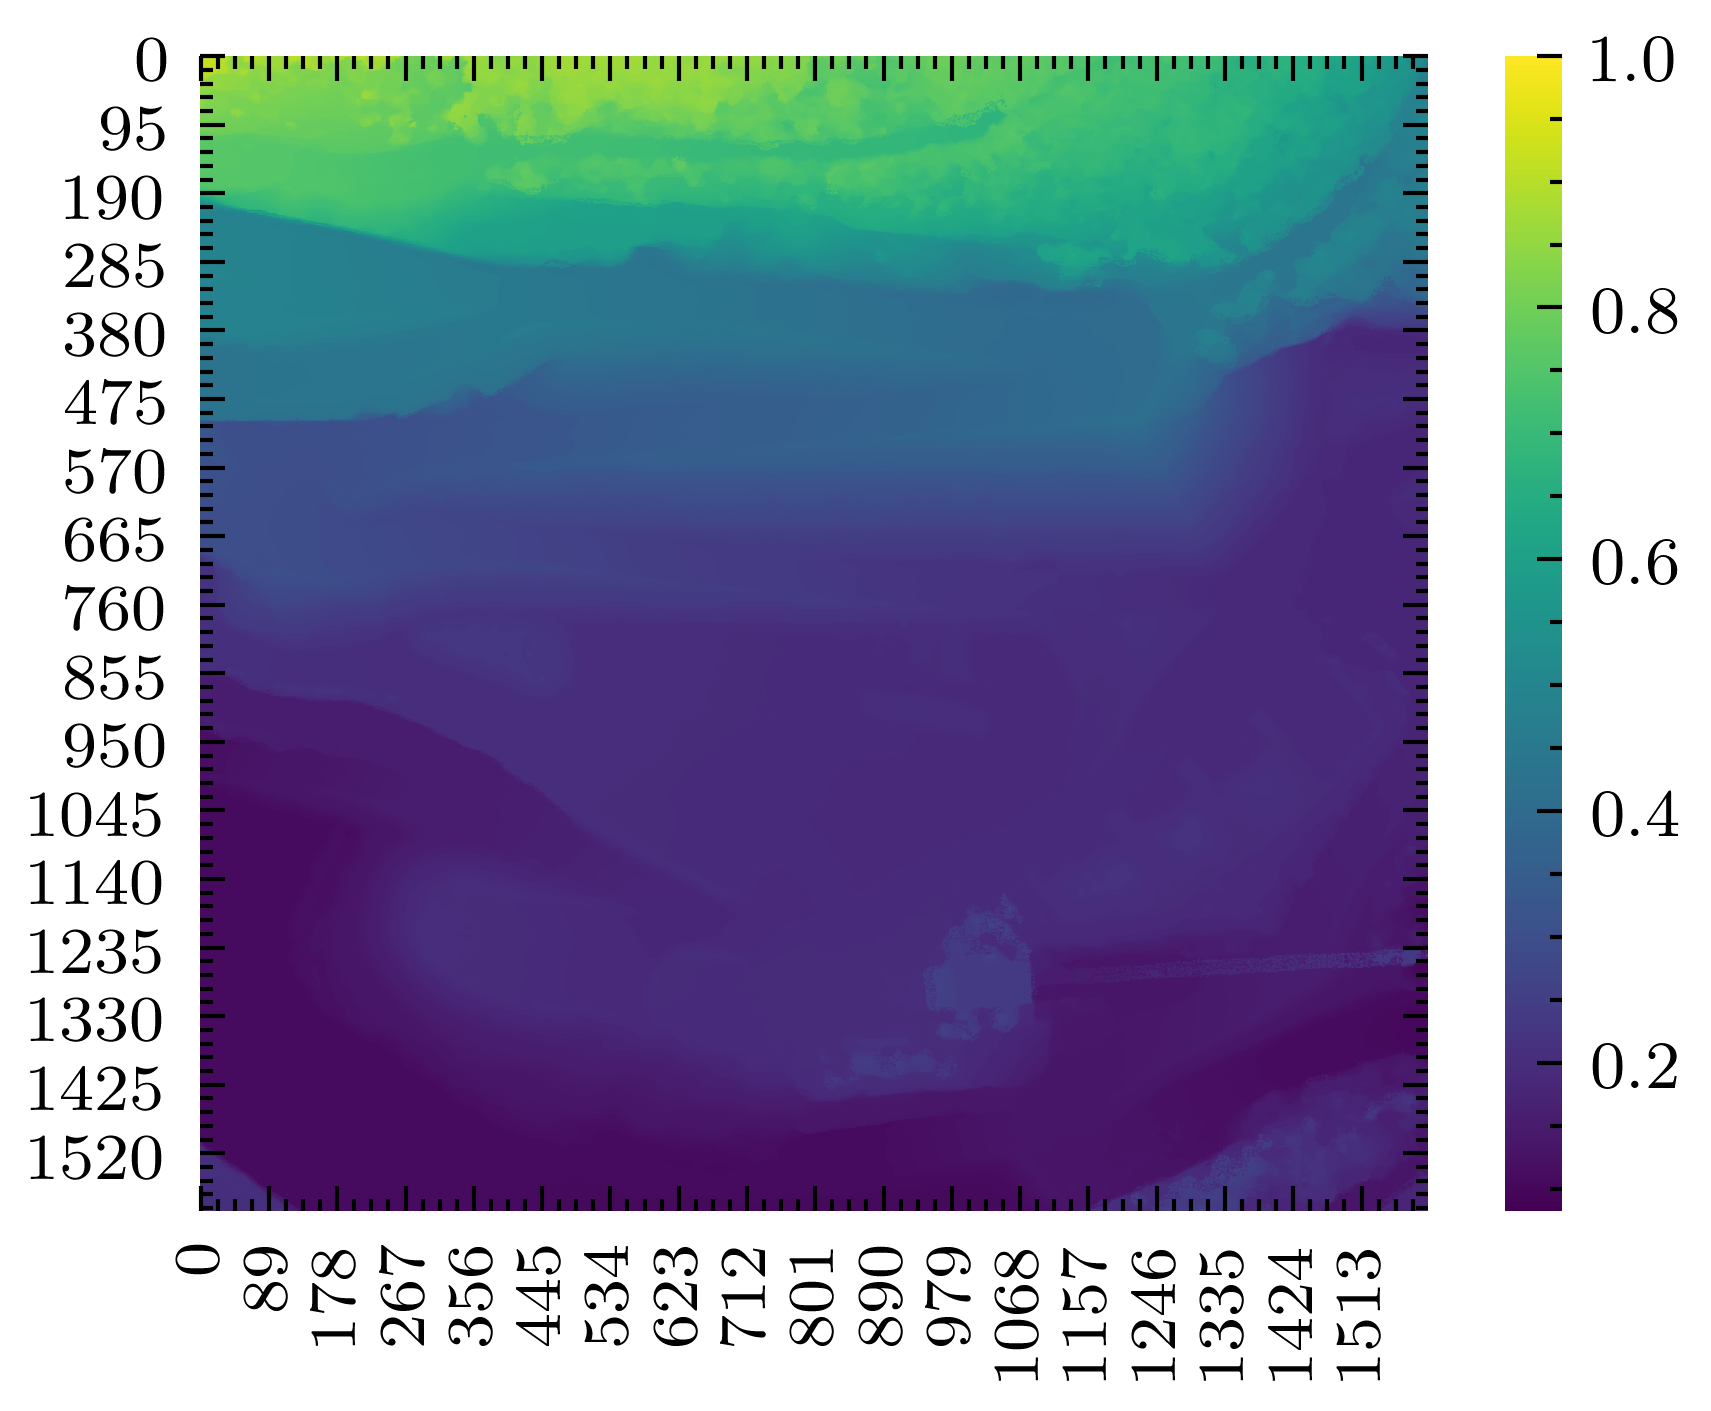
\includegraphics[width=\textwidth]{../img/hm/querry-big-10.png}
            \caption{\emph{Quarry} heightmap}
        \end{subfigure}
        \begin{subfigure}[b]{0.45\linewidth}
            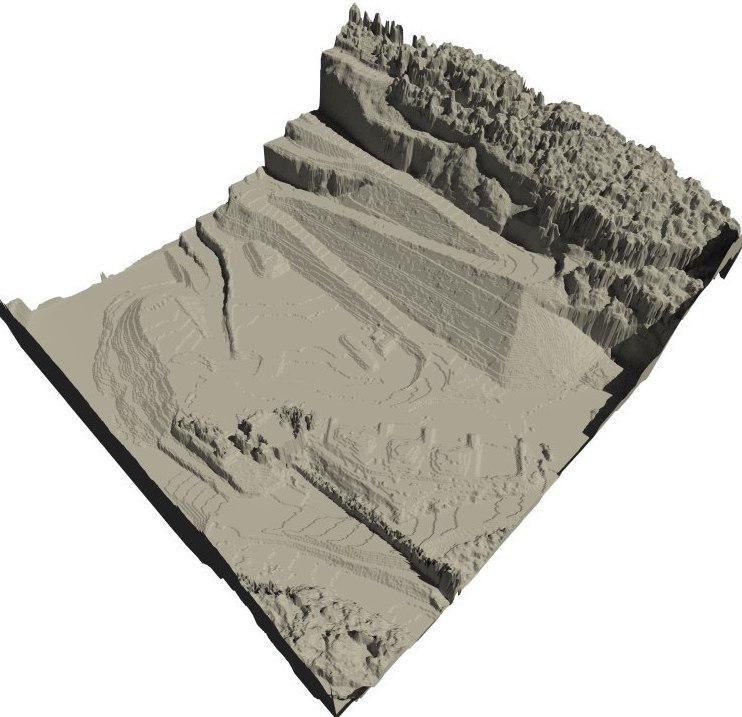
\includegraphics[width=\textwidth]{../img/quarry-rendered.png}
            \caption{\emph{Quarry} rendered}
            \end{subfigure}    
    \end{figure}
We generate fifteen terrain using random 2D simplex noise \cite{simplex}, a variant of Perlin noise \cite{perlin}, a widely used technique in terrain generation litterature.
\todo[inline]{3d rendered heightmap from Blender should visualize better the idea}
\begin{figure}[H]
    \centering
        \begin{subfigure}[b]{0.45\textwidth}
            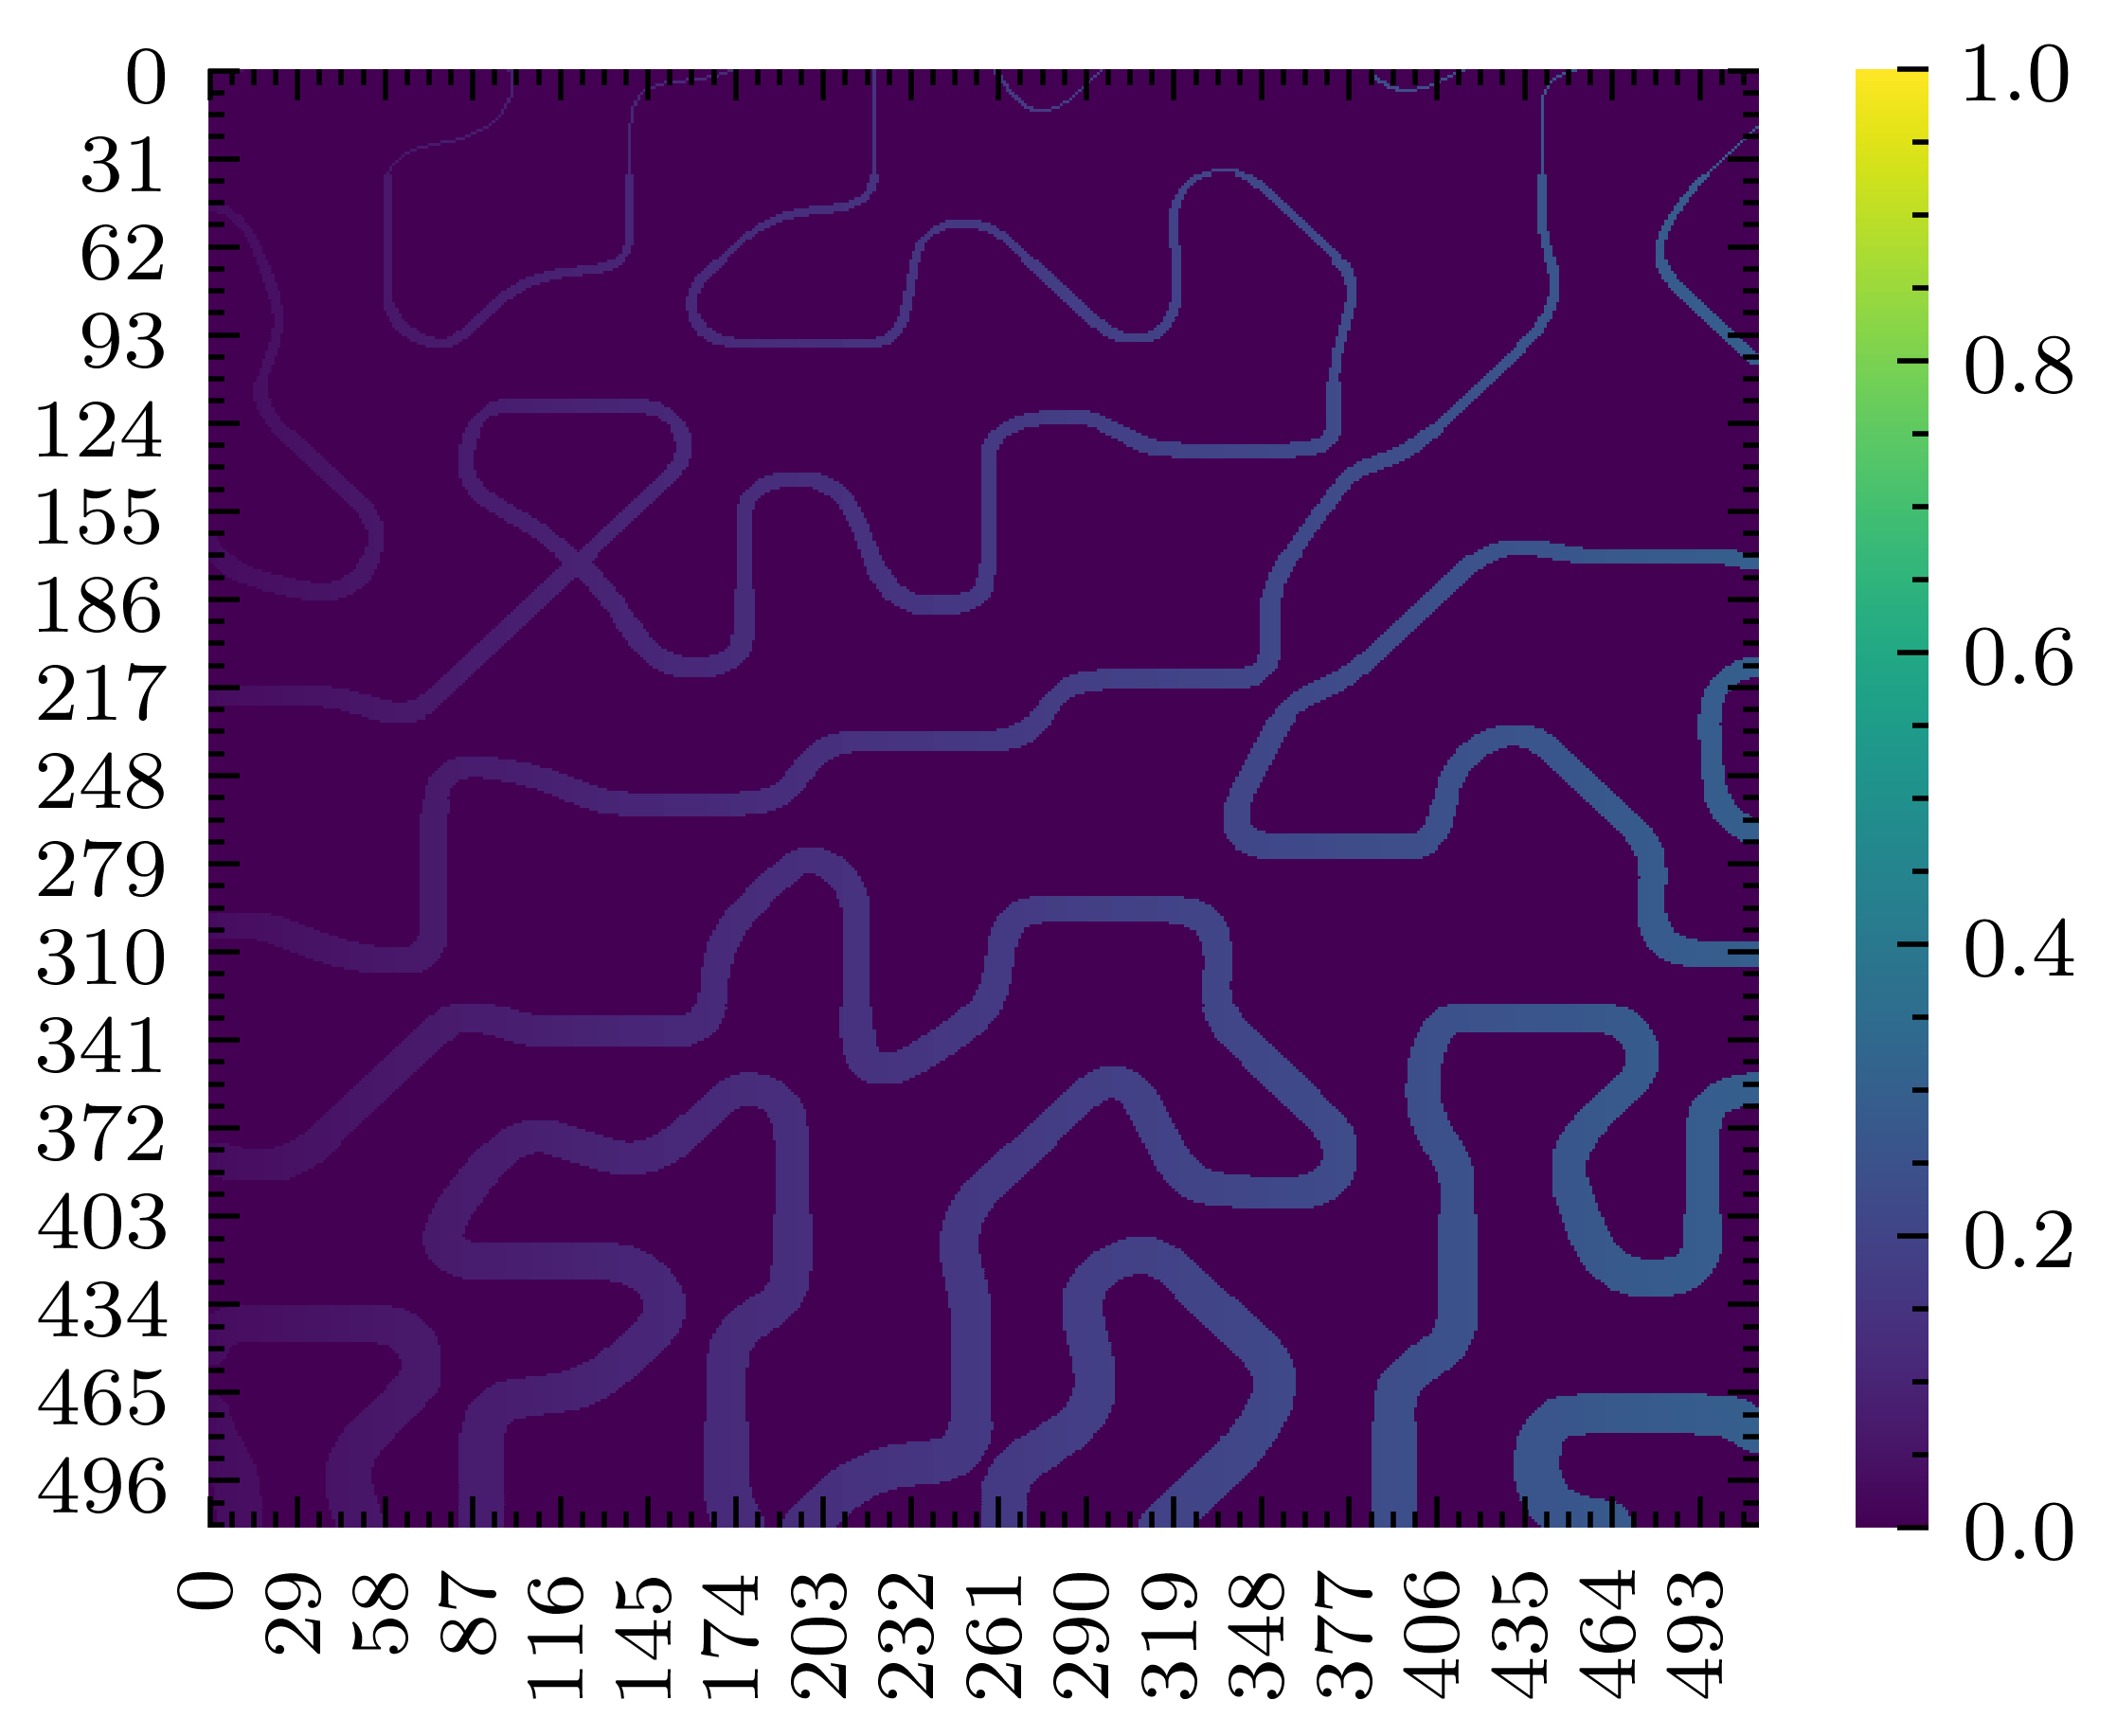
\includegraphics[width=\textwidth]{../img/hm/bars1.png}
            \caption{\emph{bars1}}
        \end{subfigure}
        \begin{subfigure}[b]{0.45\linewidth}
            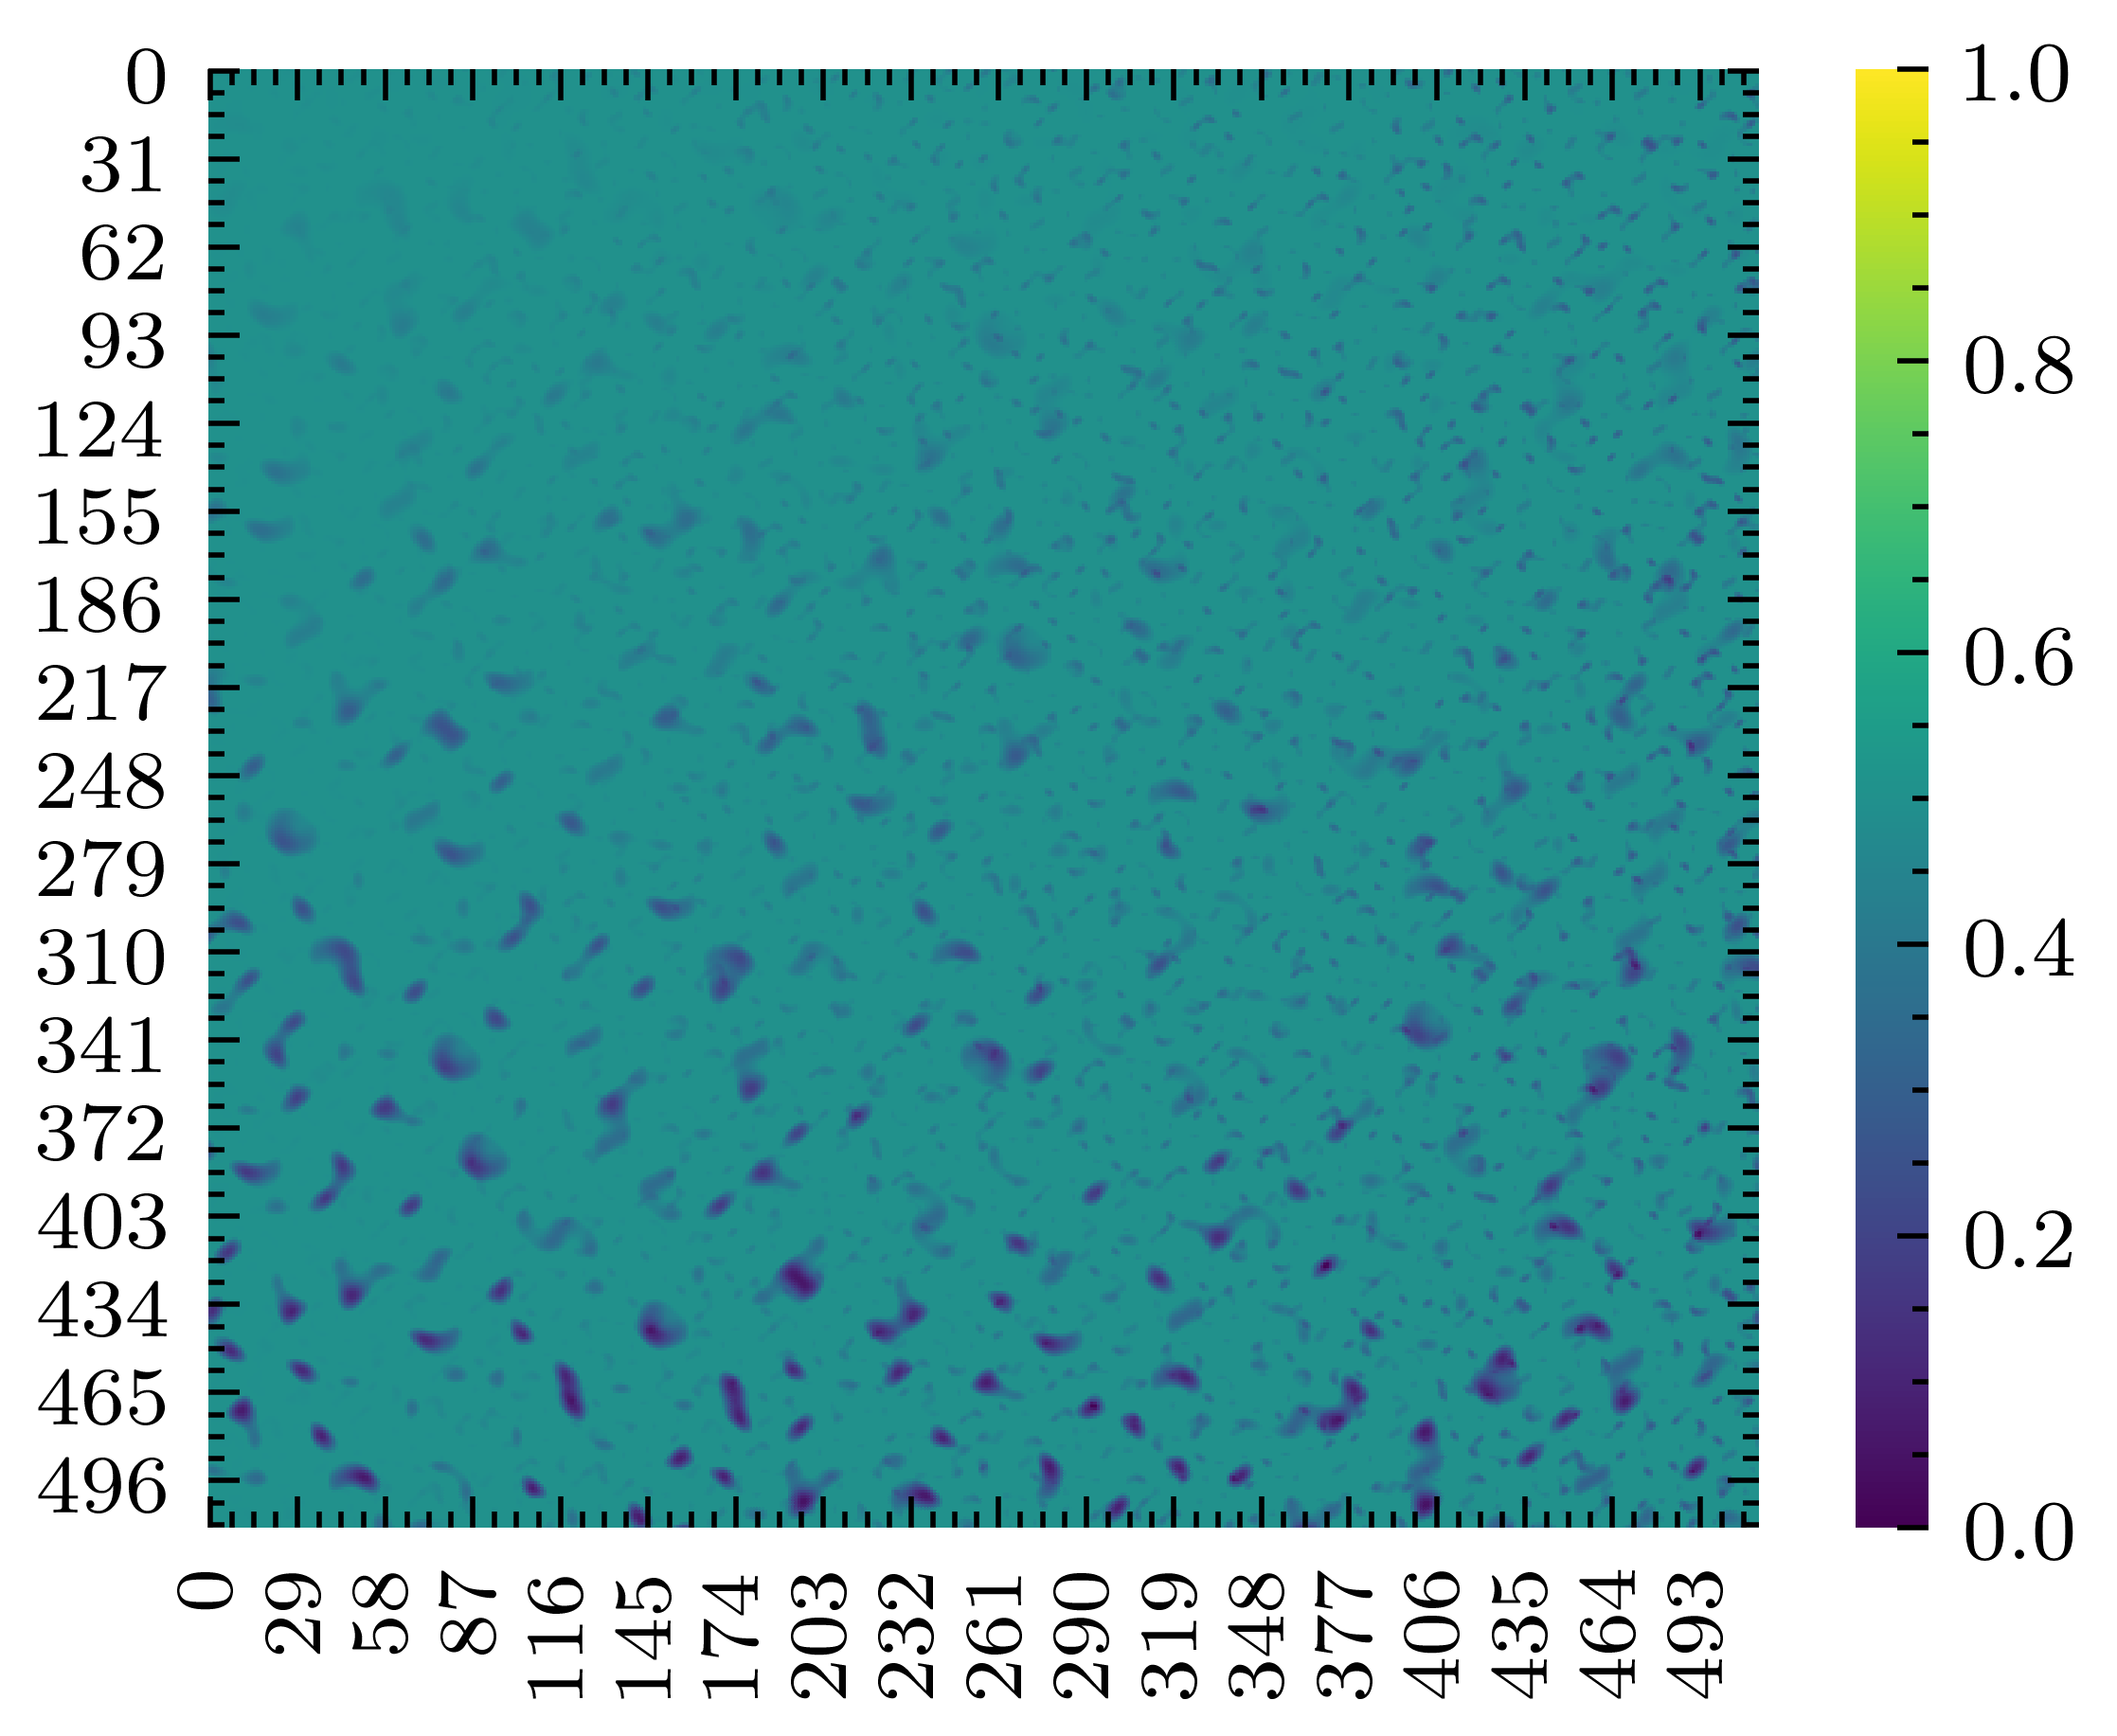
\includegraphics[width=\textwidth]{../img/hm/holes1.png}
            \caption{\emph{holes1}}
            \end{subfigure}    
          \begin{subfigure}[b]{0.45\textwidth}
            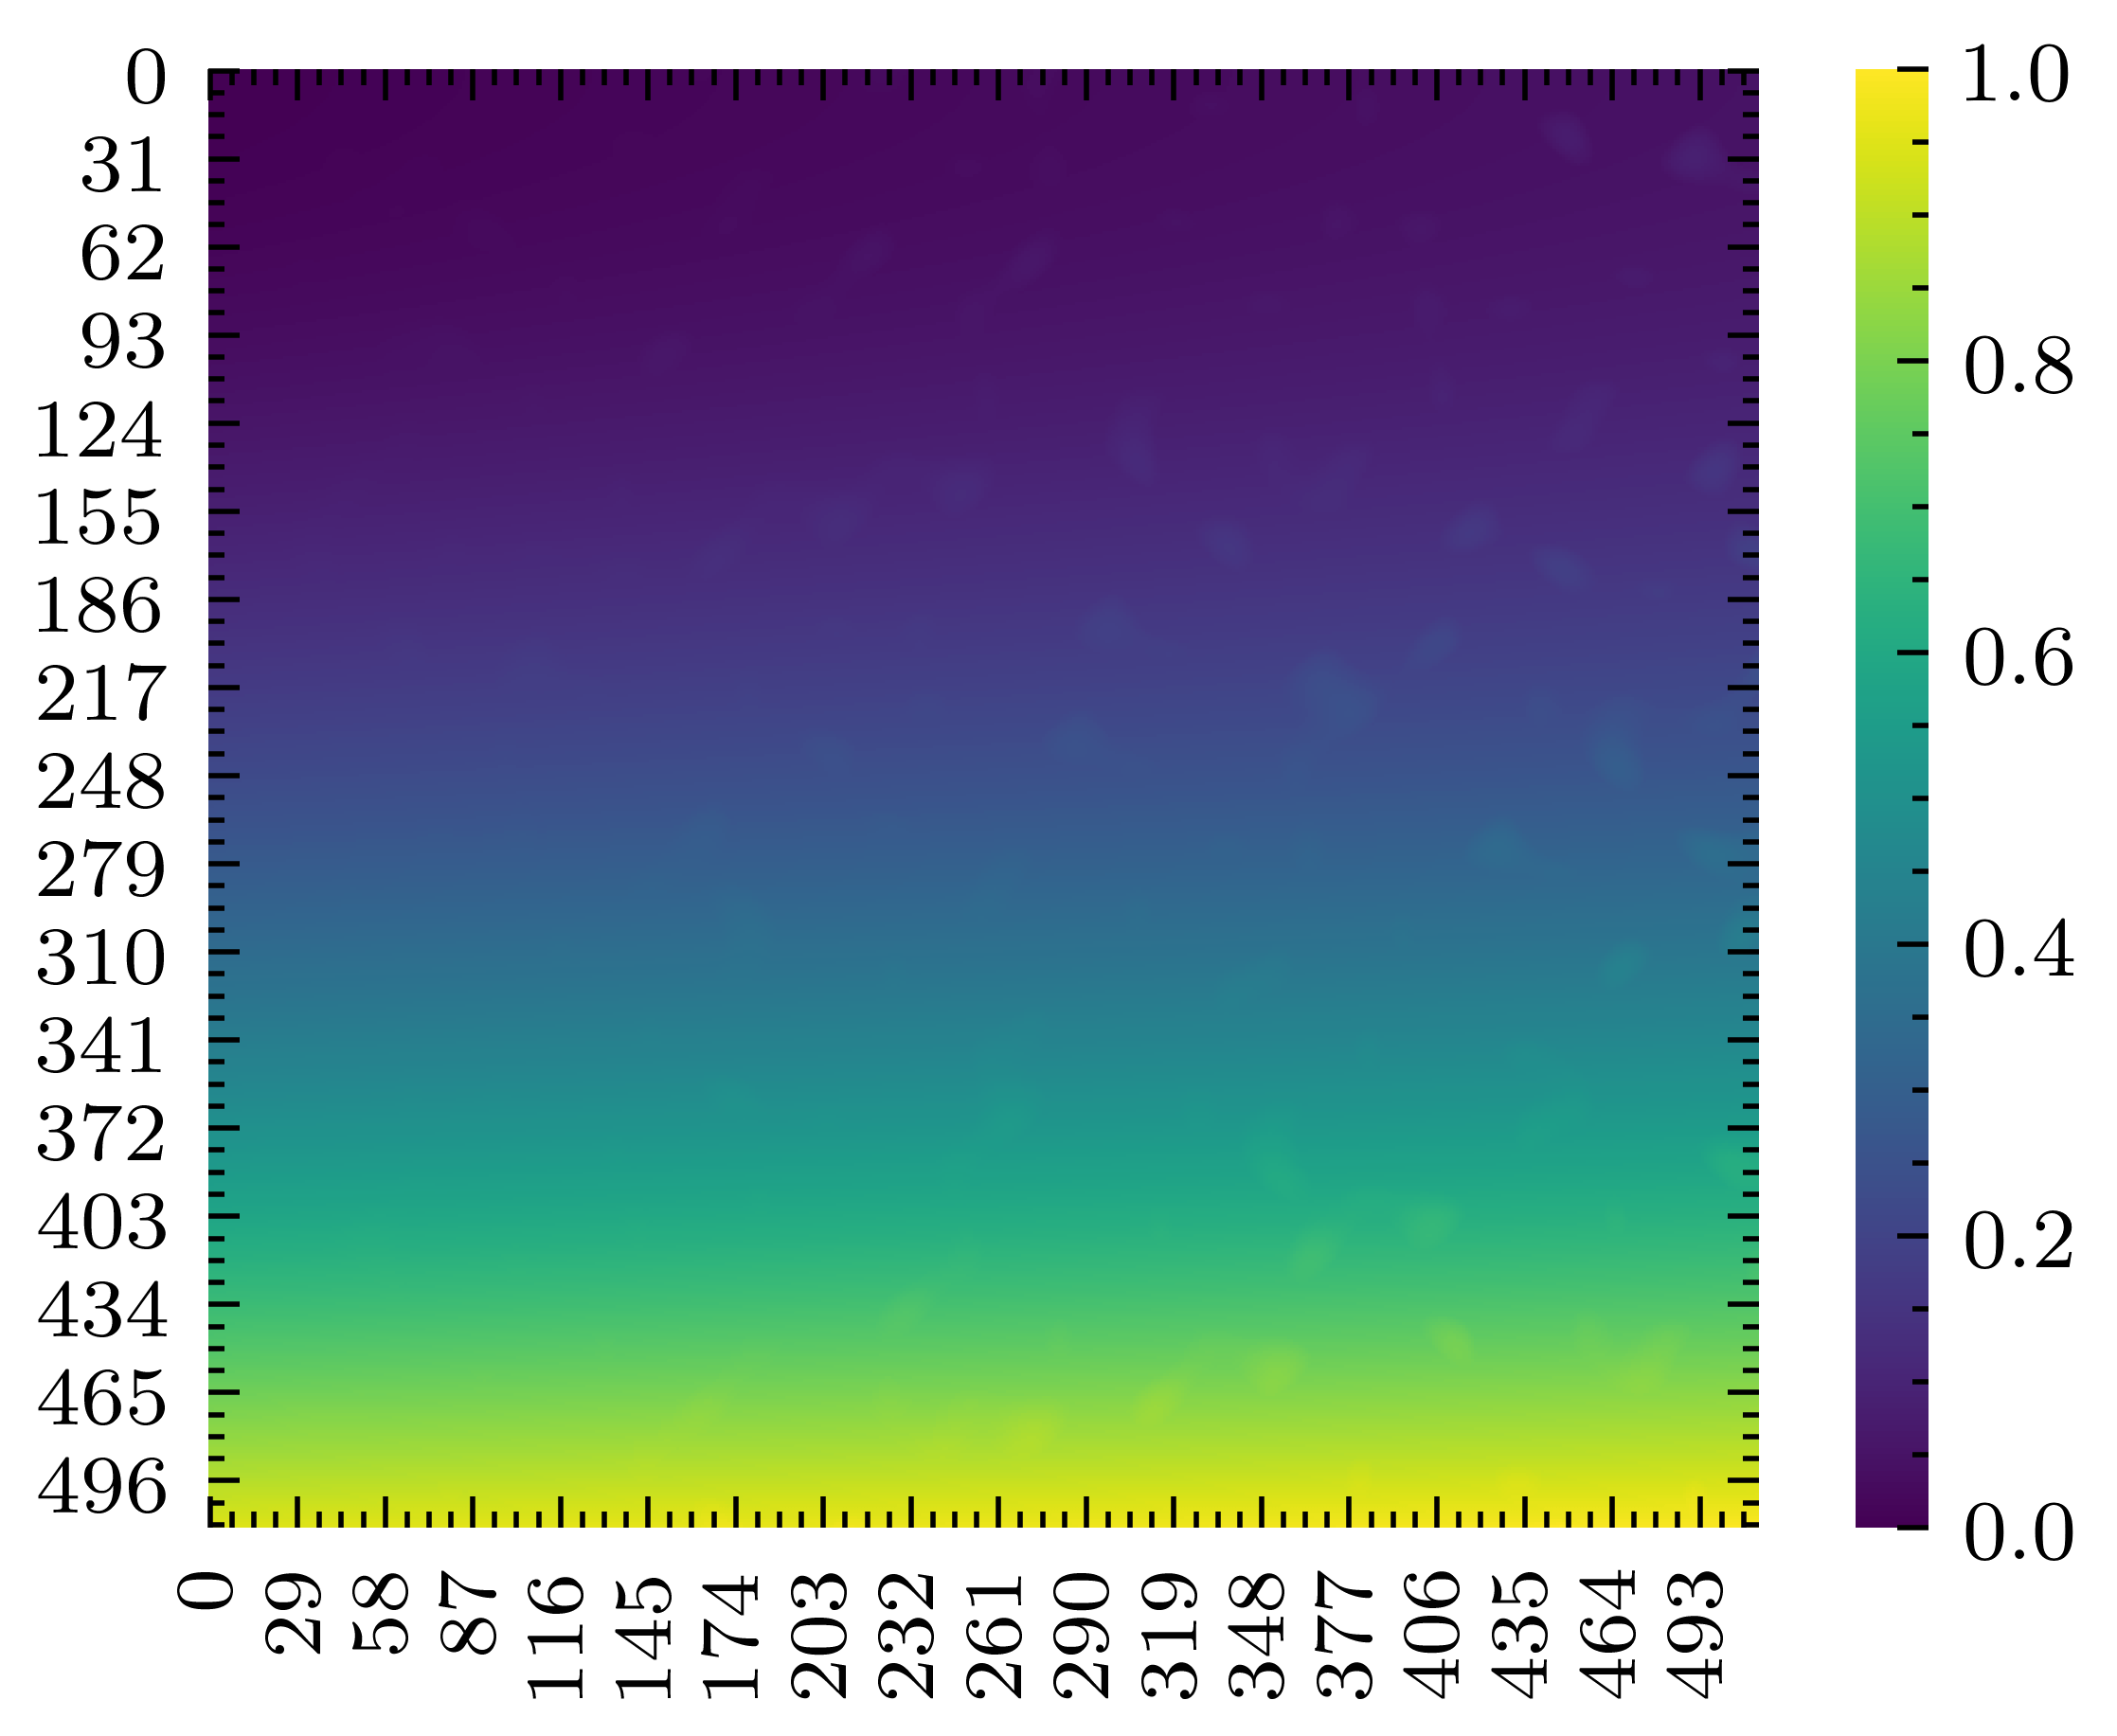
\includegraphics[width=\textwidth]{../img/hm/slope_rocks1.png}
            \caption{\emph{slope\_rocks1}}
        \end{subfigure}    
        \begin{subfigure}[b]{0.45\textwidth}
            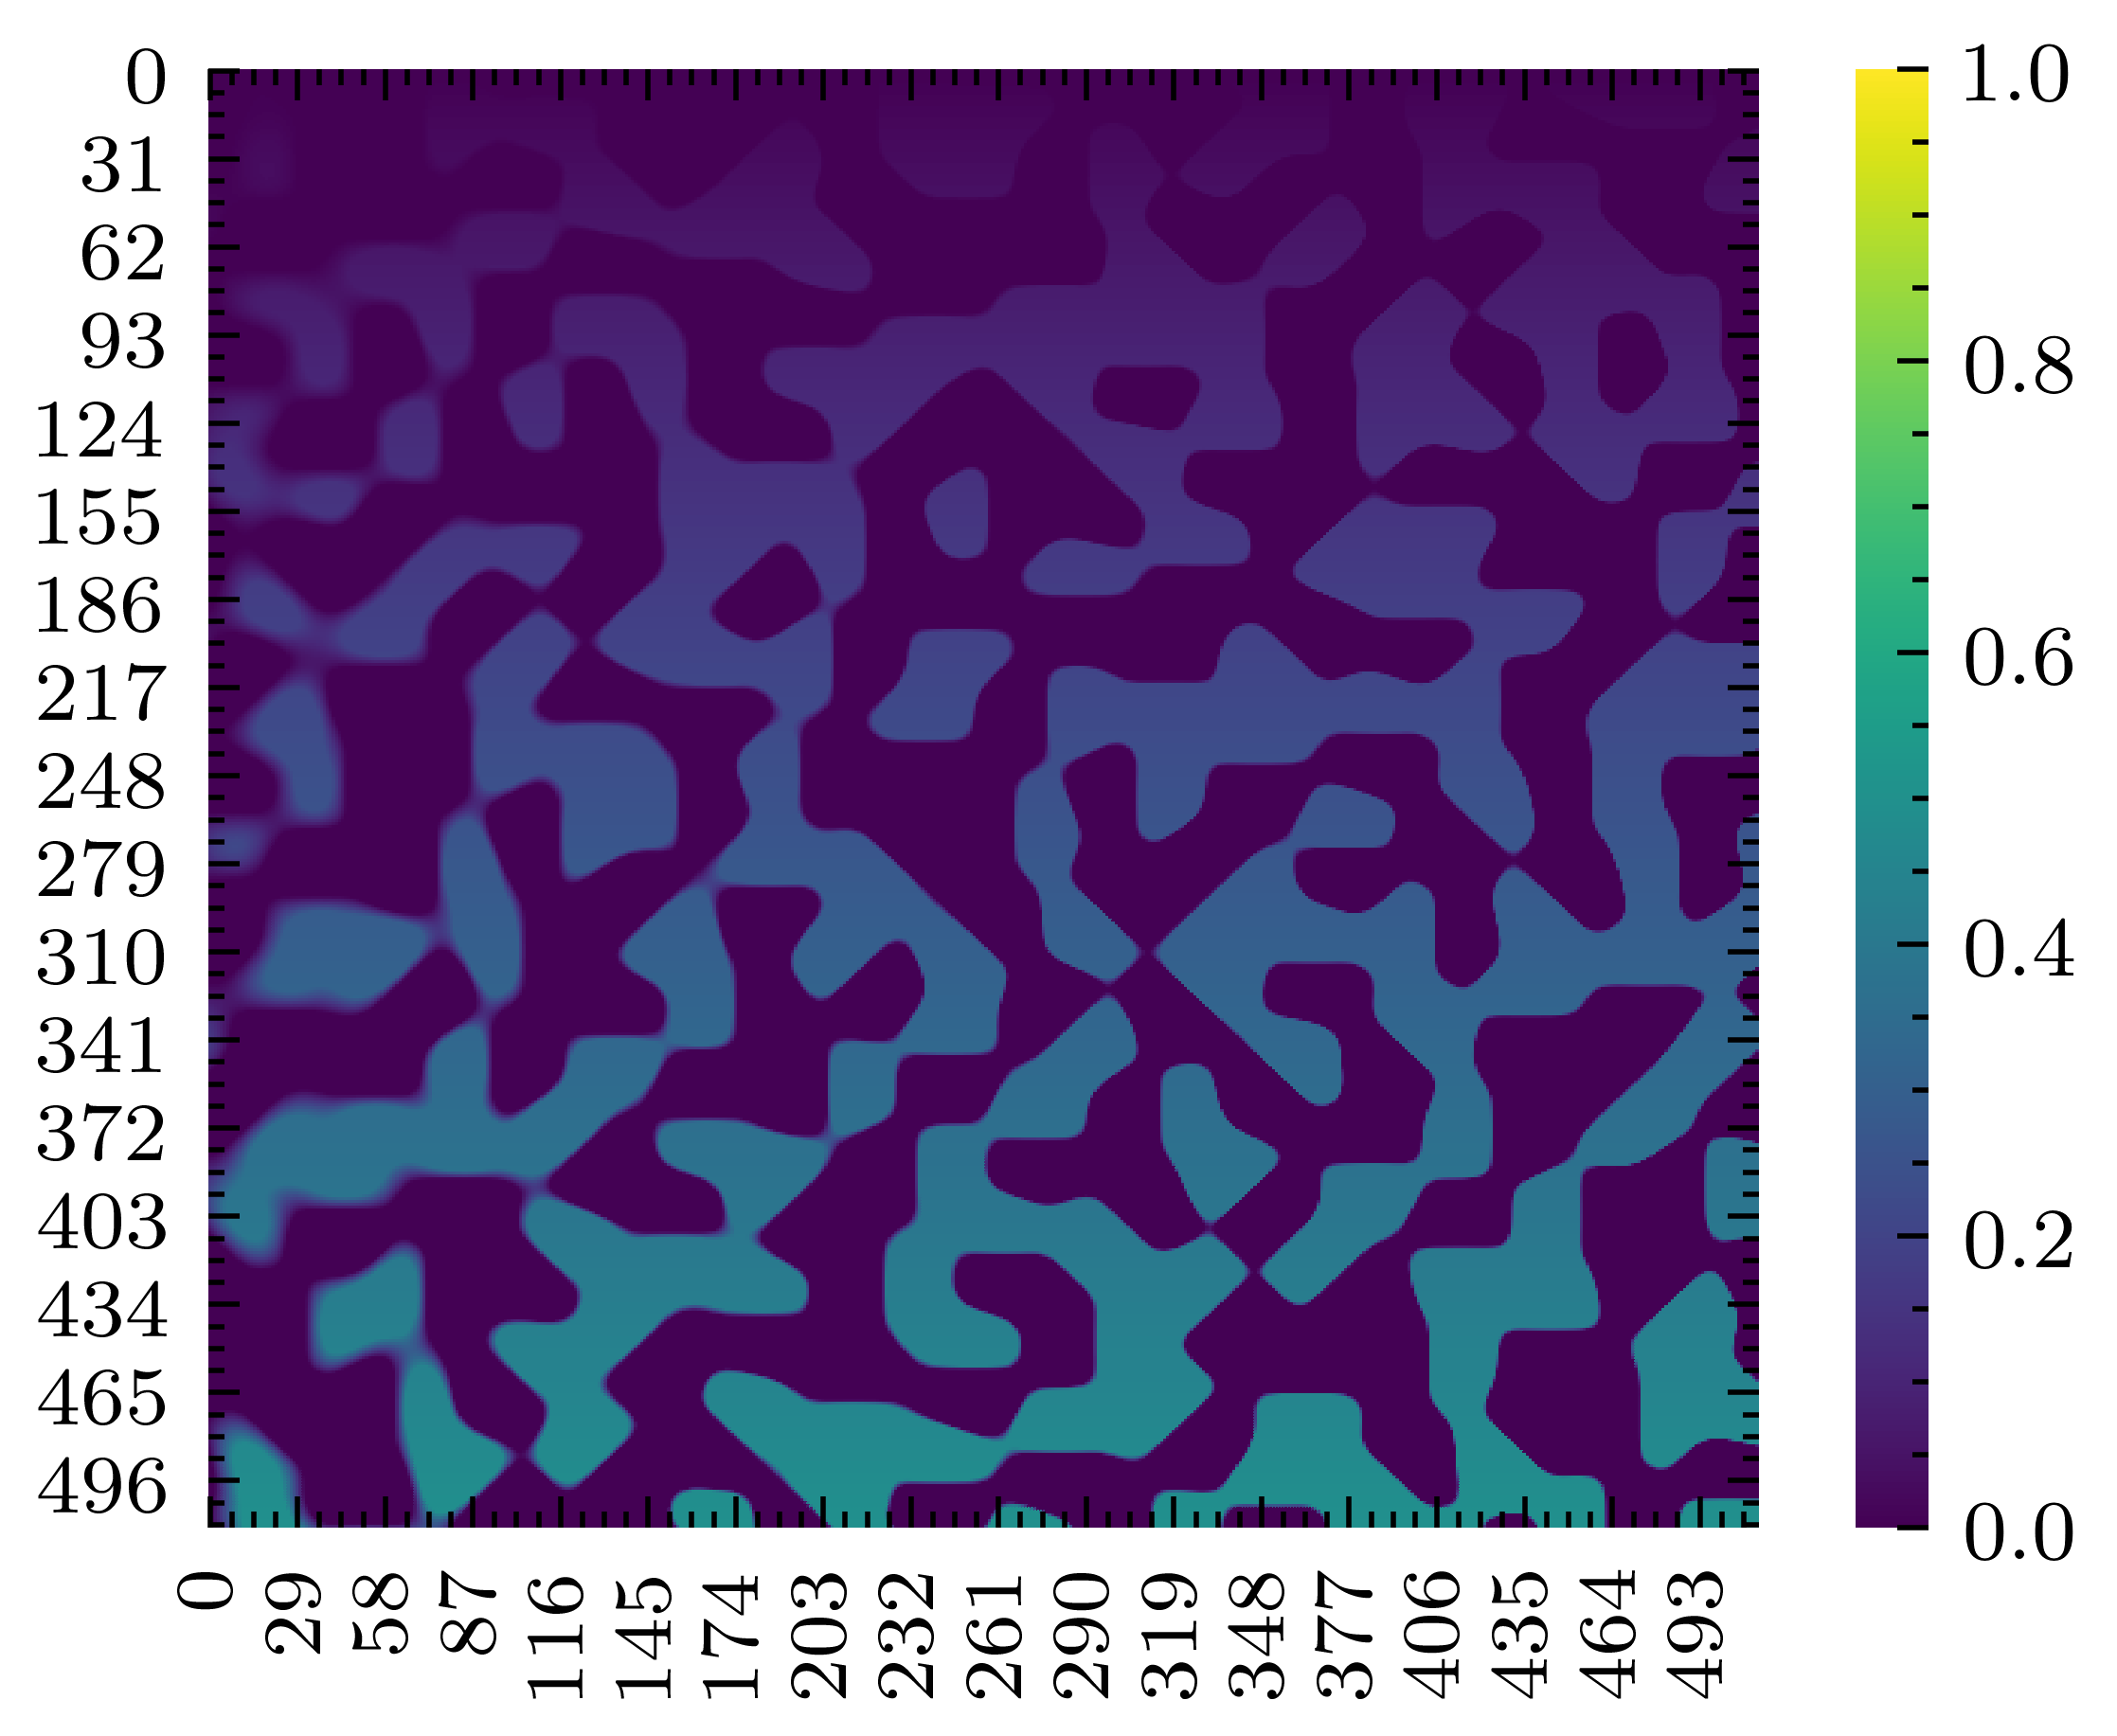
\includegraphics[width=\textwidth]{../img/hm/steps1.png}
            \caption{\emph{steps1}}
        \end{subfigure}    
    \label{fig: heightmaps}
    \caption{Some of the synthetic heightmaps}
\end{figure}
\subsubsection{Simulator}
We used Webots to move \emph{Krock} on the genereted terrain. The robot controlled was implemented by EPFL \todo{cite them?} and handed to IDSIA \todo{cite?}. The controller implements a ROS' node to publish \emph{Krock} status including its pose at a rate of $250hz$. We decide to reduce it $50hz$ by using ROS build it \texttt{throttle} command. 
To load the map into the simulator we had to convert it to Webots's \emph{.wbt} file. Unfortunately, the simulator lacks support for heightmap so we had to use a script to read the image and perform the conversion.

To communicate with the simulator, Webots exposes a wide number of ROS services, similar to HTTP endpoints, with which we can communicate. To call one service, we first have to get the correct type of message we wish to send and then we can call it. We decided to implement a little library called \emph{webots2ros} \todo{link} to perform this call automatically making the code cleaner and more intuitive. 

We also implement one additional library called \emph{agent} \todo{link} to create reusable robot's interfaces independent from the simulator. The package supports callbacks that can be attached to each agent adding additional features. Finally, we used \emph{Gym} \cite{gym}, a toolkit to develop and evaluate reinforcement learning algorithms, to define our environment. Due to the library's popularity,  the code can easily be shared with other researches or we may directly experiment with already made RL algorithm in the future without changing the code.

\subsubsection{Simulation}
To collect \emph{Krock}'s interaction with the environment, we spawn it on the ground and let it move forward for $20$ seconds. We repeat this process fifty times per each map.
    Unfortunately, spawning the robot is not a trivial task. In certain maps, for instance, \emph{bars1}, we must avoid spawning on an obstacle otherwise the run will be ruined because \emph{Krock} will be stuck form the start and we will introduce unwanted noise in the dataset. To solve the problem, we define a random spawn strategy used in most of the maps without big obstacles such as $slope_rocks$, and a flat ground spawn strategy for the others. The random spawn just selects a random position and rotation for the robot. On the other hand, the flat ground strategy first selects suitable spawn positions by using a sliding window on the heightmap of size equal \emph{Krock}'s footprint and check if the mean pixel value is lower than a small threshold. If so, we store the center coordinates of the patch. Intuitively, if a patch is flat the mean valu will be close to zero.
    
We clustered those points with K-Means in $k$ clusters where $k$ is the number of spawning points we need, in our case fifty. By clustering, we guarantee to cover all region of the map. The following picture shows this strategy on \emph{bars1}.

\begin{figure}[H]
    \begin{subfigure}[b]{0.5\textwidth}
        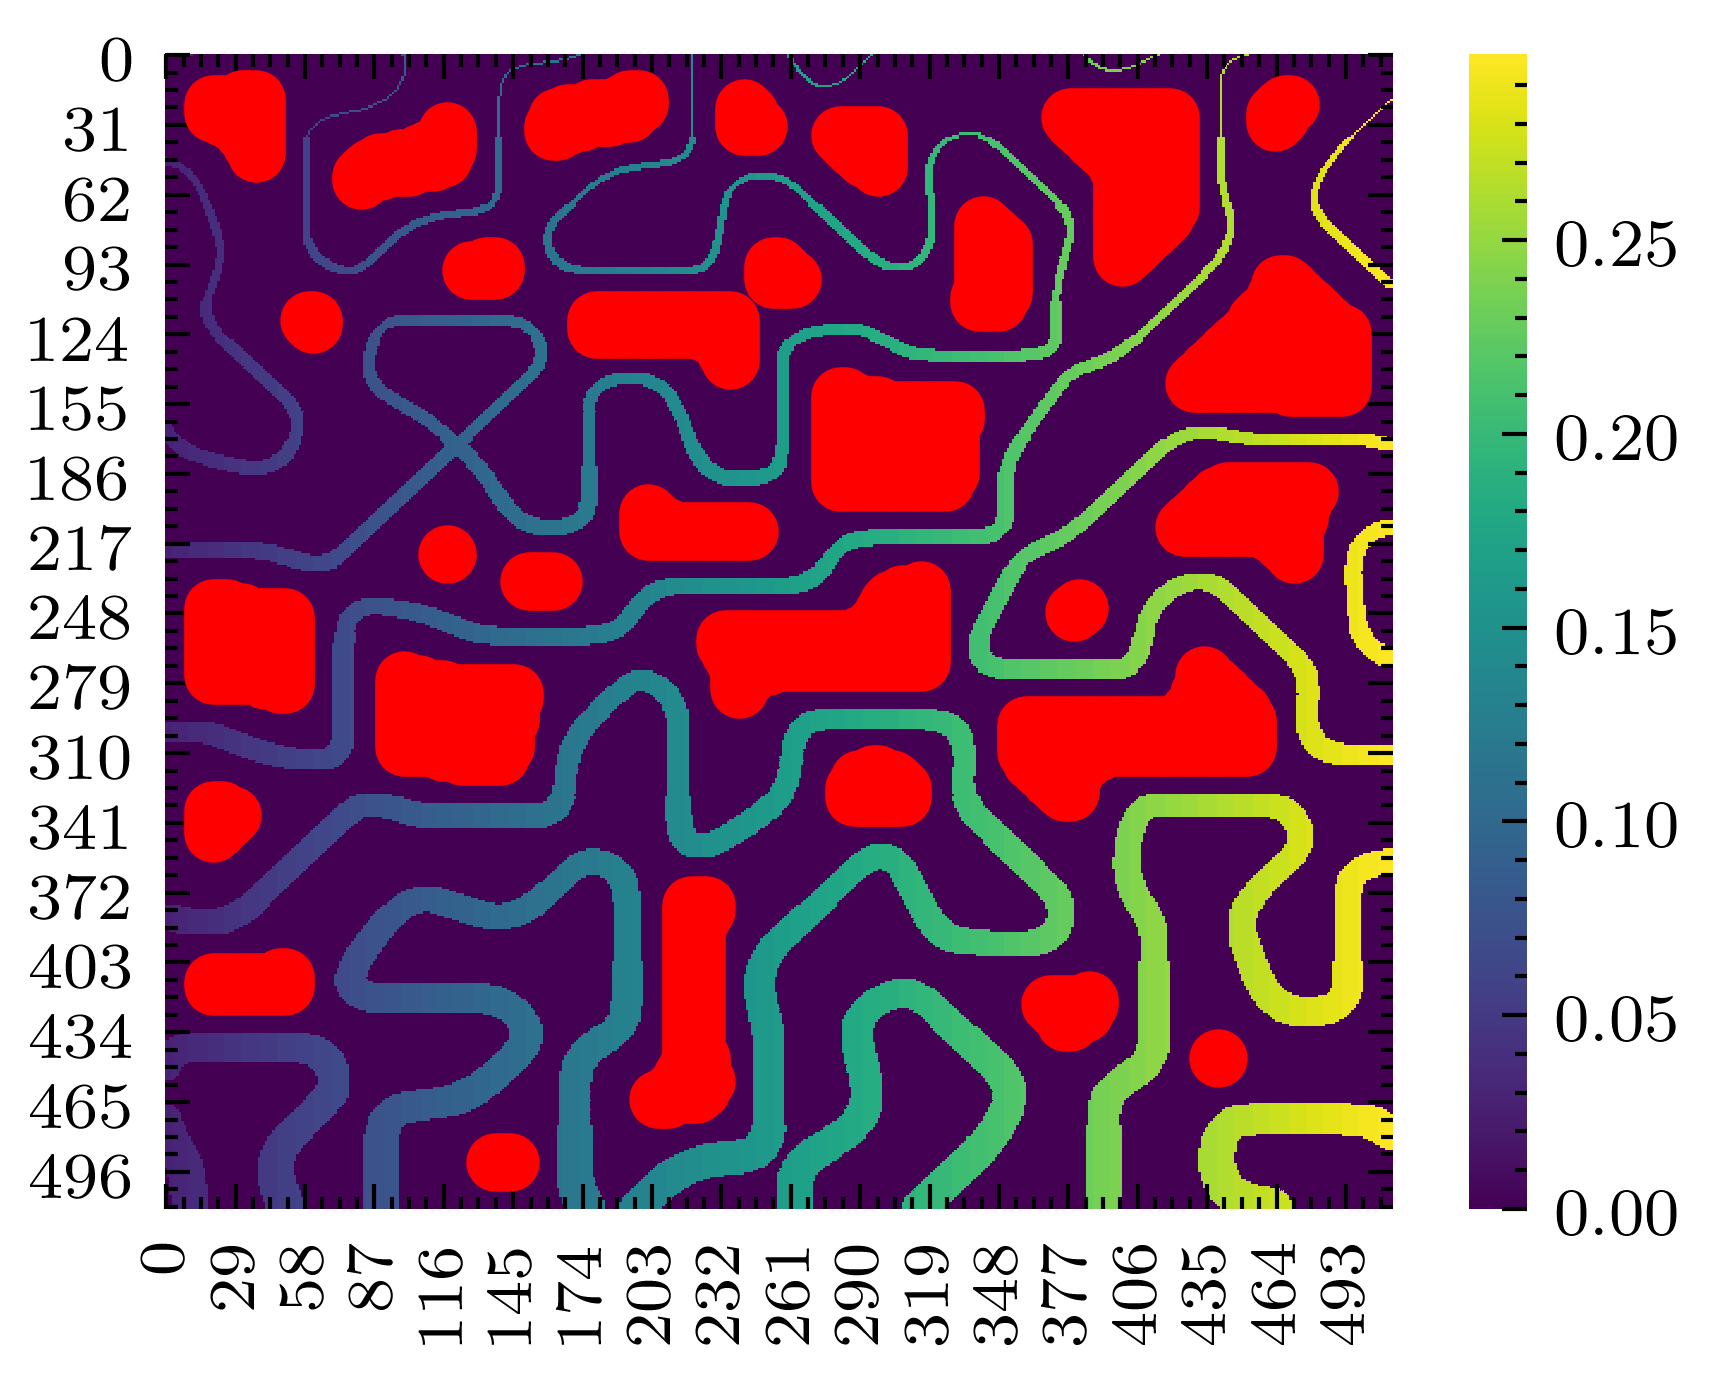
\includegraphics[width=\textwidth]{../img/3/spawn/flat-spawn-10.png}
        \caption{Flat regions}
    \end{subfigure}
    \begin{subfigure}[b]{0.5\textwidth}
        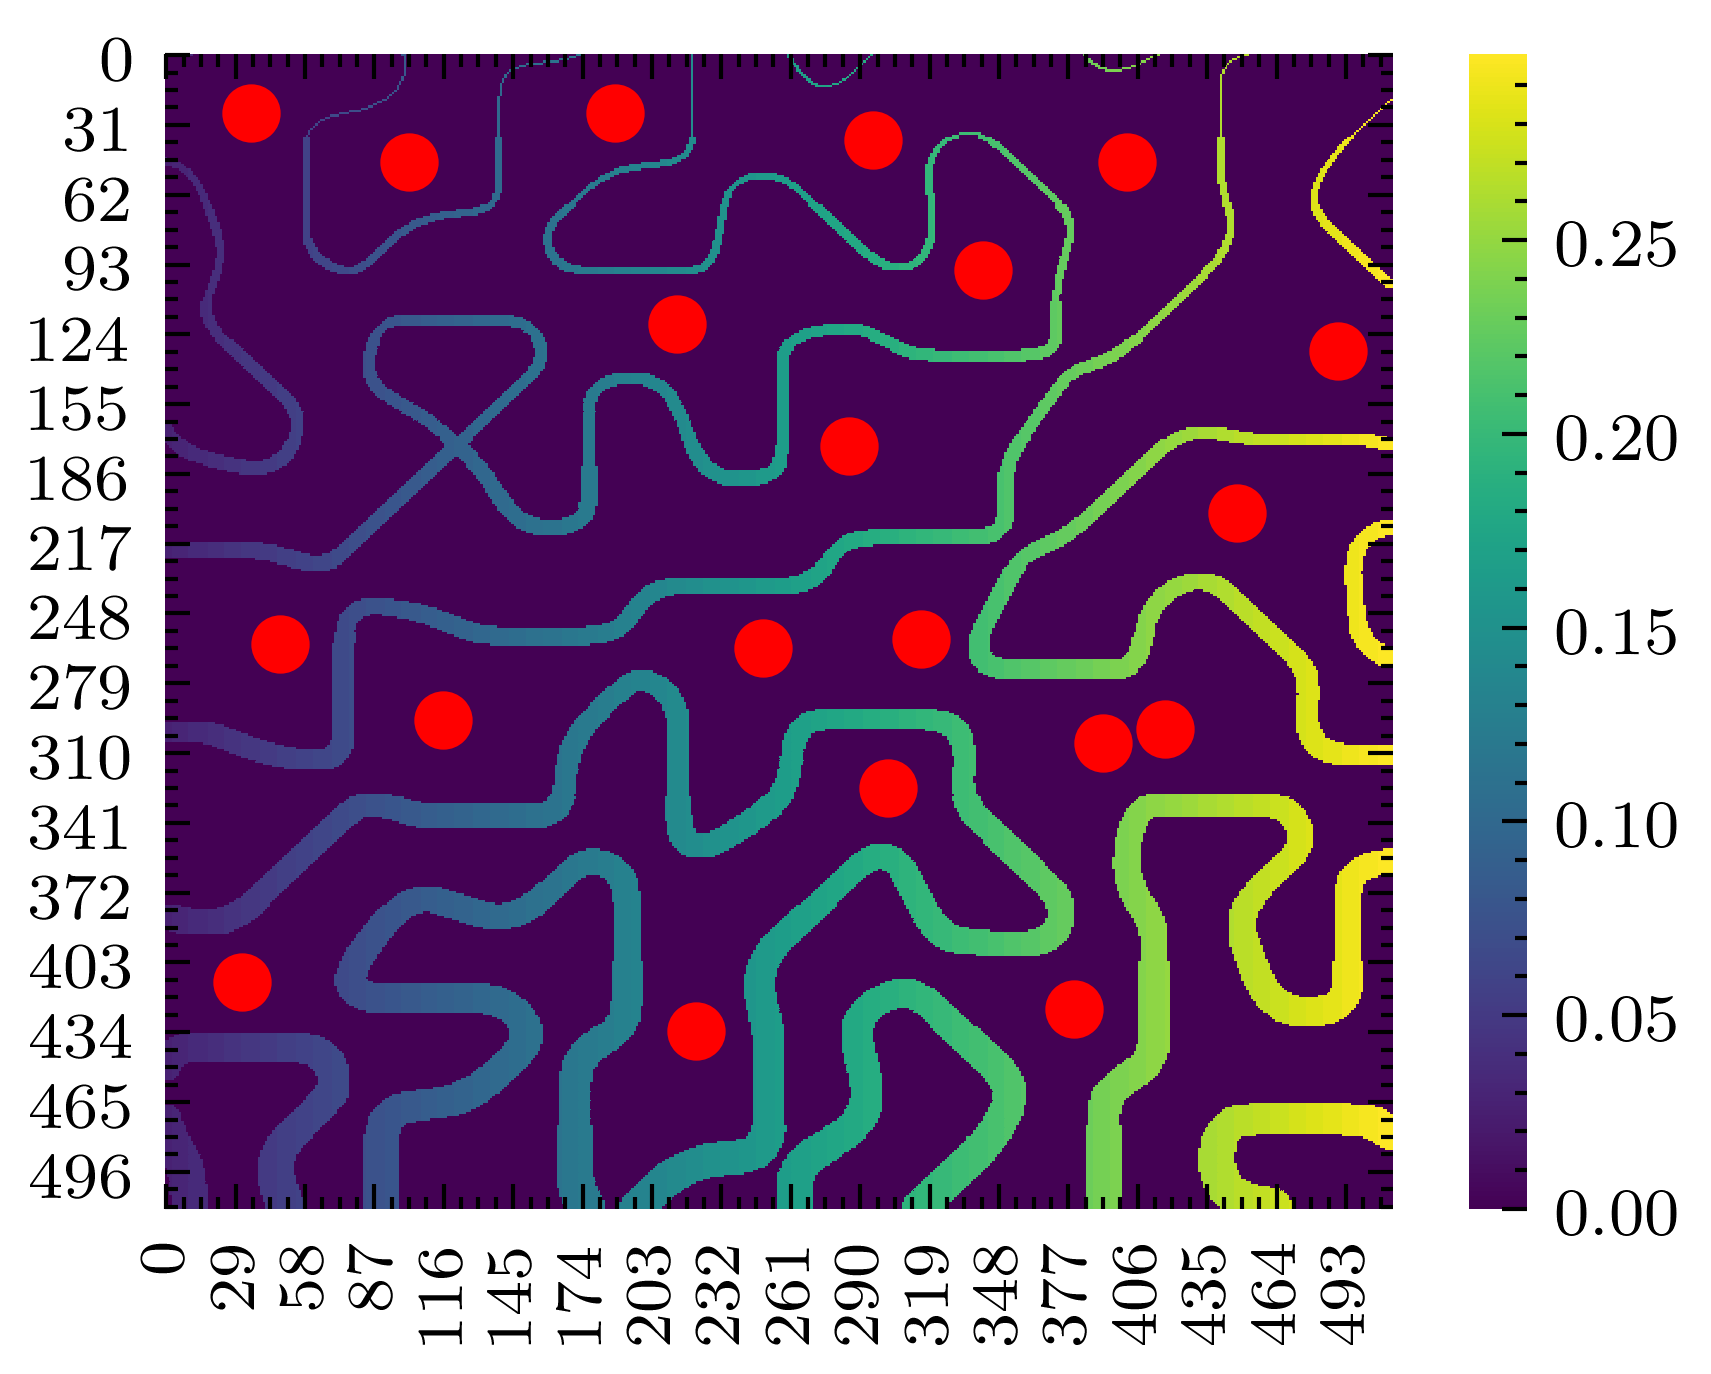
\includegraphics[width=\textwidth]{../img/3/spawn/spawn-10.png}
        \caption{K-Means with $k=20$}
    \end{subfigure}  
\label{fig: spawn-strat}
\caption{Selecting $20$ spawning points in \emph{bars1}}    
\end{figure}


\subsection{Postprocessing}
We now need to extract the patches for each pose $p_t$ of \emph{Krock} and compute the advancement for a given time window. To create the post-processing pipeline, we create an easy to use API \todo{link to the project} to define a cascade stream of function that is applied one after the other using a multi-thread queue to speed-up the process

First, we turn each \emph{.bag} file to a pandas dataframe and cache them into \emph{.csv} files. We used an open source library we ported to python3 to perform the conversion.\todo{library that converts the bags file}.
Then, we load the dataframes with the respective heightmaps and start the data cleaning process. We remove the rows corresponding tp the first second of the simulation time to account for the robot spawning time. Then we eliminate all the entries where the \emph{Krock} pose was near the edges of a map, we used a threshold of $22$ pixels since we notice  \emph{Krock} getting stuck in the borders of the terrain during a simulation. 
After cleaning the data, we convert \emph{Krock}quaternion rotation to Euler notation using the \emph{tf} package \todo{link to tf transform} from ROS. Then, we extract the $\sin$ and $\cos$ from the Euler orientation last component and store them in a column.
Before caching again the resulting dataframes into \emph{.csv} files, we convert the robot's position into heightmap's coordinates used later to crop the correct region of the map.

Finally, we load again the last stage and compute the advancement by projecting the pose's position, $x$ and $y$, in the current line. Then, we select a time window according to the store rate, for if we select two seconds we need to multiply the rate by two, so $50*2=100$ since \emph{Krock} published with a $50hz$ frequency. Once the time window is defined, we project $x$ and $y$ on the current line used the $\sin$ and $\cos$ values calculated before to get the advancement.

To create the patches, we first discover the maximum advancement for one second by running some simulations of \emph{Krock} on flat ground and averaging the advancement. For our robot, the maximum speed is $33cm/s$ Then, we multiply the maximum displacement by the number of seconds we are interested in. We can now crop the corresponding region in the heightmap by including the whole \emph{Krock}'s footprint and the maximum advancement. The following figure visualizes the patch extraction process. 
\todo[inline]{figure that shows Krock somewhere with the patch bounding boxed}. Lastly, we create a final dataframe containing the map coordinates, the advancement, and the patches paths for each simulation and store them to disk as \emph{.csv} files. 

The whole pipeline takes less than one hour to run the first time with 16 threads, and, once it is cached, less than fifteen minutes to extract the patches. 

Once we extract the patches, we can always re-compute the advancement without re-running the whole pipeline. The next figure show proposed pipeline.
\begin{figure}[H] 
\centering
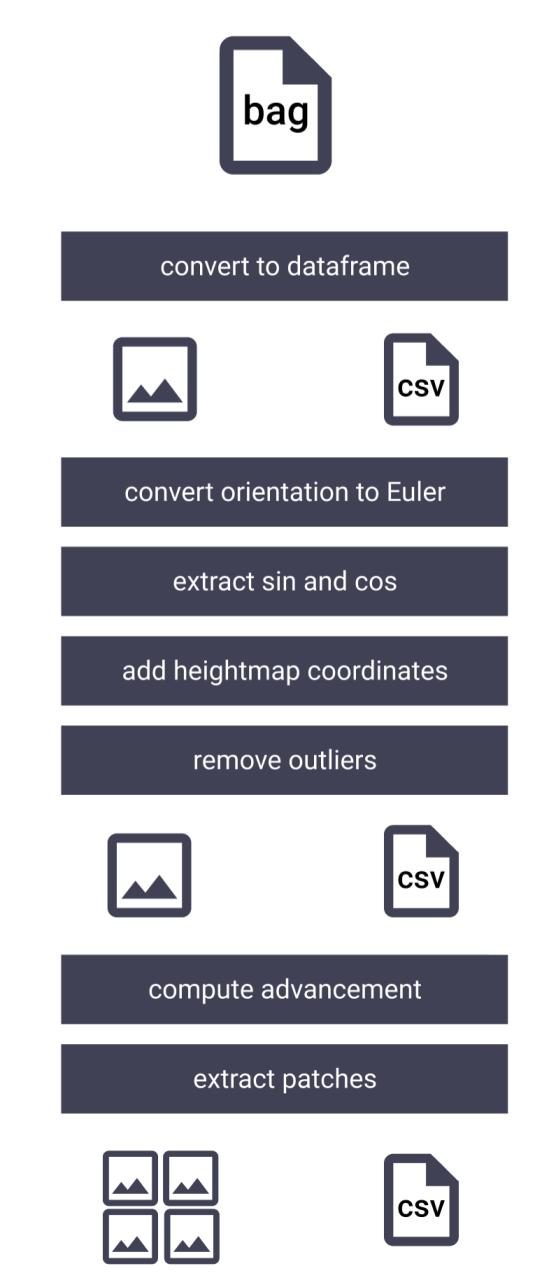
\includegraphics[width=0.4\textwidth]{../img/postprocessing-pipeline.jpg}
\caption{Postprocessing}
\label{fig: postprocessing-pipeline}
\end{figure}
\subsection{Estimator}

\subsubsection{Vanilla Model}
\subsubsection{ResNet}

We decide to use a Residual Network, ResNet \cite{he2015deep}, variant. Residual networks are deep convolutional
networks consisting of many stacked \" Residual Units \". Intuitively, the residual unit allows the input of a layer to contribute to the next layer's input by being added to the current layer's output. Due to possible different features dimension, the input must go through and identify map to make the addition possible. This allows a stronger gradient flows and mitigates the degradation problem. A \"Residual Units \" is composed by a two $3x3$ \emph{Convolution}, \emph{Batchnorm} \cite{ioffe2015batch} and a \emph{Relu} blocks. Formally, it is defined as: 
\begin{equation}
    \mathbf{y}=\mathcal{F}\left(\mathbf{x},\left\{W_{i}\right\}\right)+h(\mathbf{x})
    \label{eq : resnet}
\end{equation}
Where, $x$ and $y$ are the input and output vector of the layers considered. The function $\mathcal{F}\left(\mathbf{x},\left\{W_{i}\right\}\right)$ is the residual mapping to be learn and $h$ is the identity mapping. The next figure visualises the equation.

\begin{figure}[H]
    \centering
    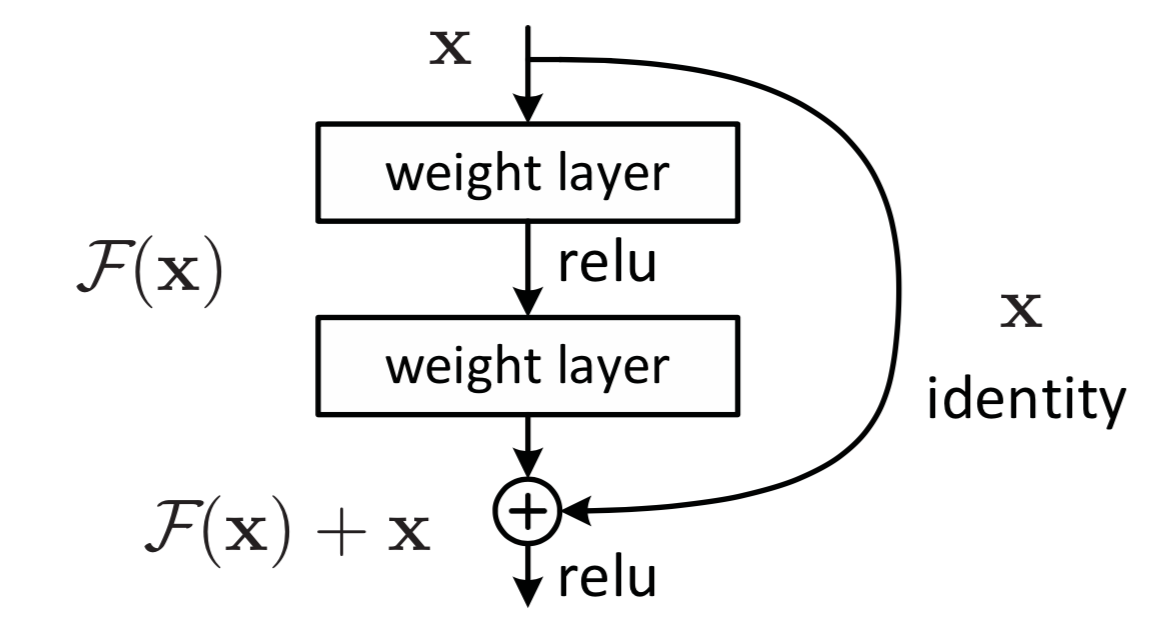
\includegraphics[scale=0.3]{../img/implementation/estimator/resnet_block.png}
    \caption{\emph{Resnet} block.}
\end{figure}
When the input and output shapes mistmatch, the \emph{identity map} is applyed to the input as a $3x3$ Convolution with a stride of 2 to mimic the polling operator. A single block is composed by a $3x3$ \emph{Convolution}, \emph{Batchnorm} and a \emph{Relu} activation function. 

Following the recent work of He et al. \cite{he2015identity} we adopt \emph{pre-activation} in each block.\emph{Pre-activation} works by just reverse the order of the operations in a block.

\begin{figure}[H]
    \centering
    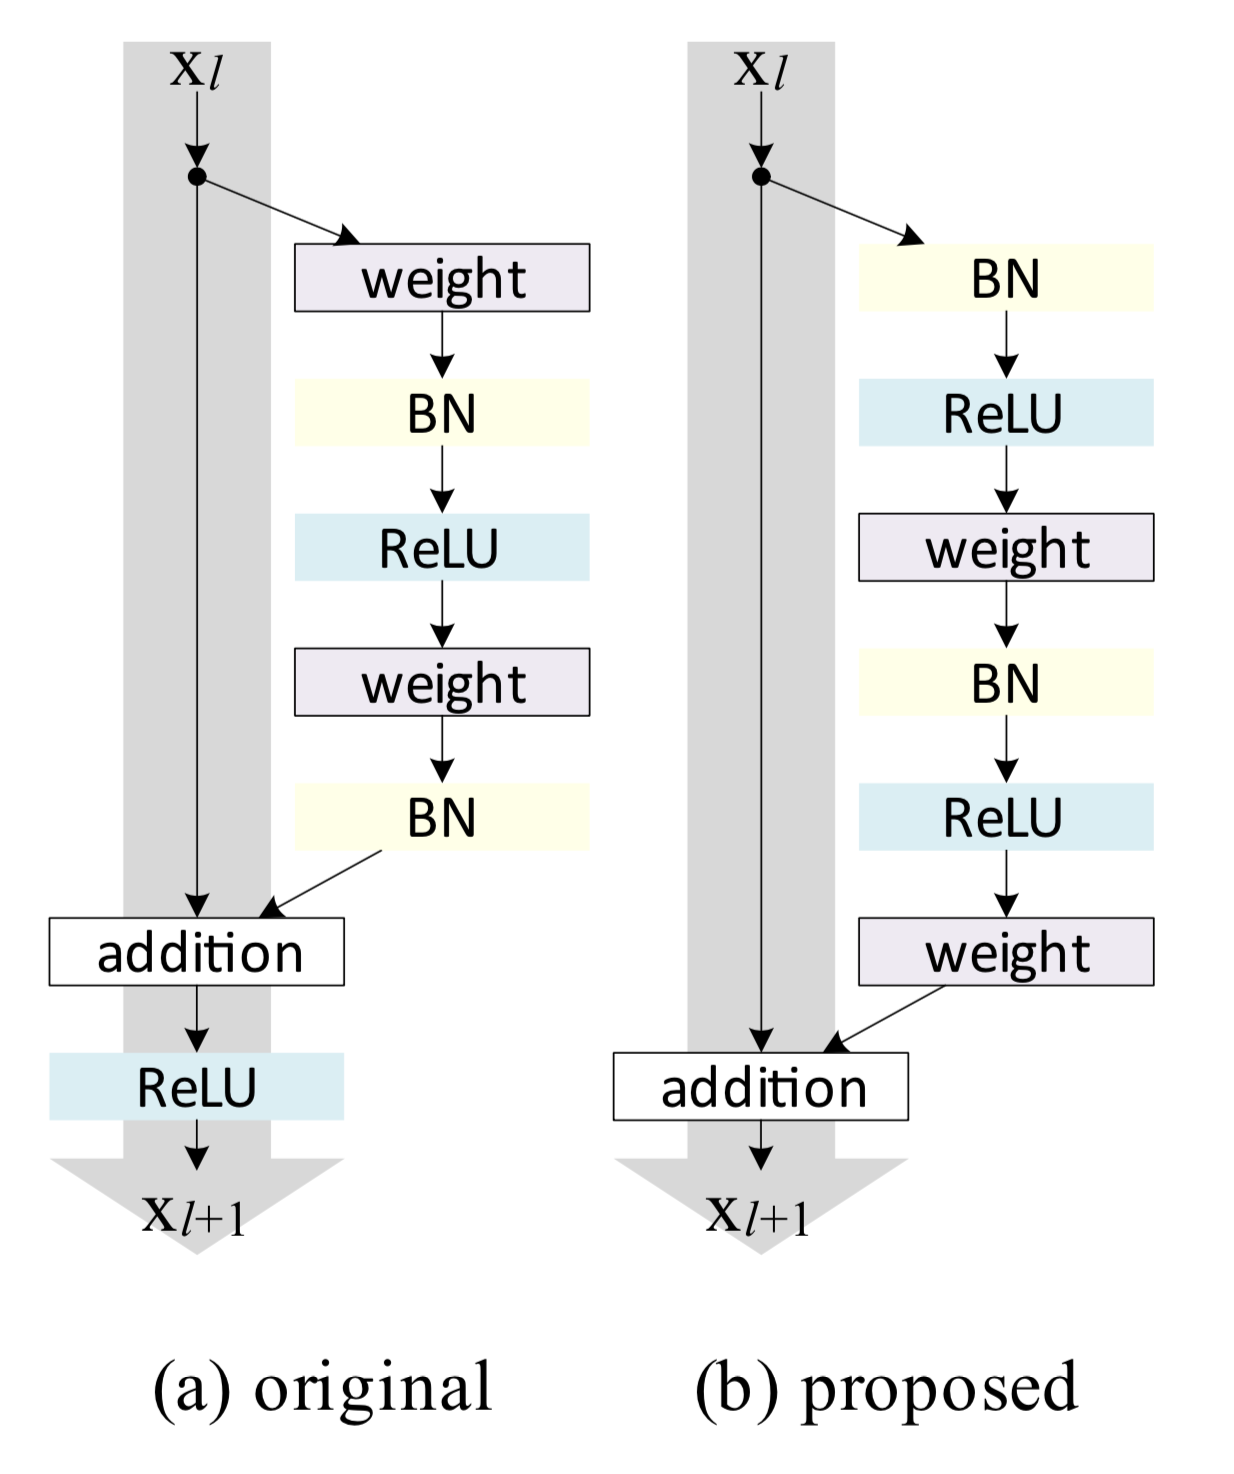
\includegraphics[scale=0.2]{../img/implementation/estimator/preactivation.png}
    \caption{\emph{Preactivation}}
\end{figure}
Finally, we also used the \emph{Squeeze and Excitation} (SE) module \cite{hu2017squeeze}. It is a form of attention that weights the channel of each convolutional operation by learnable scaling factors. The next figure visualises the SE module.
\begin{figure}[H]
    \centering
    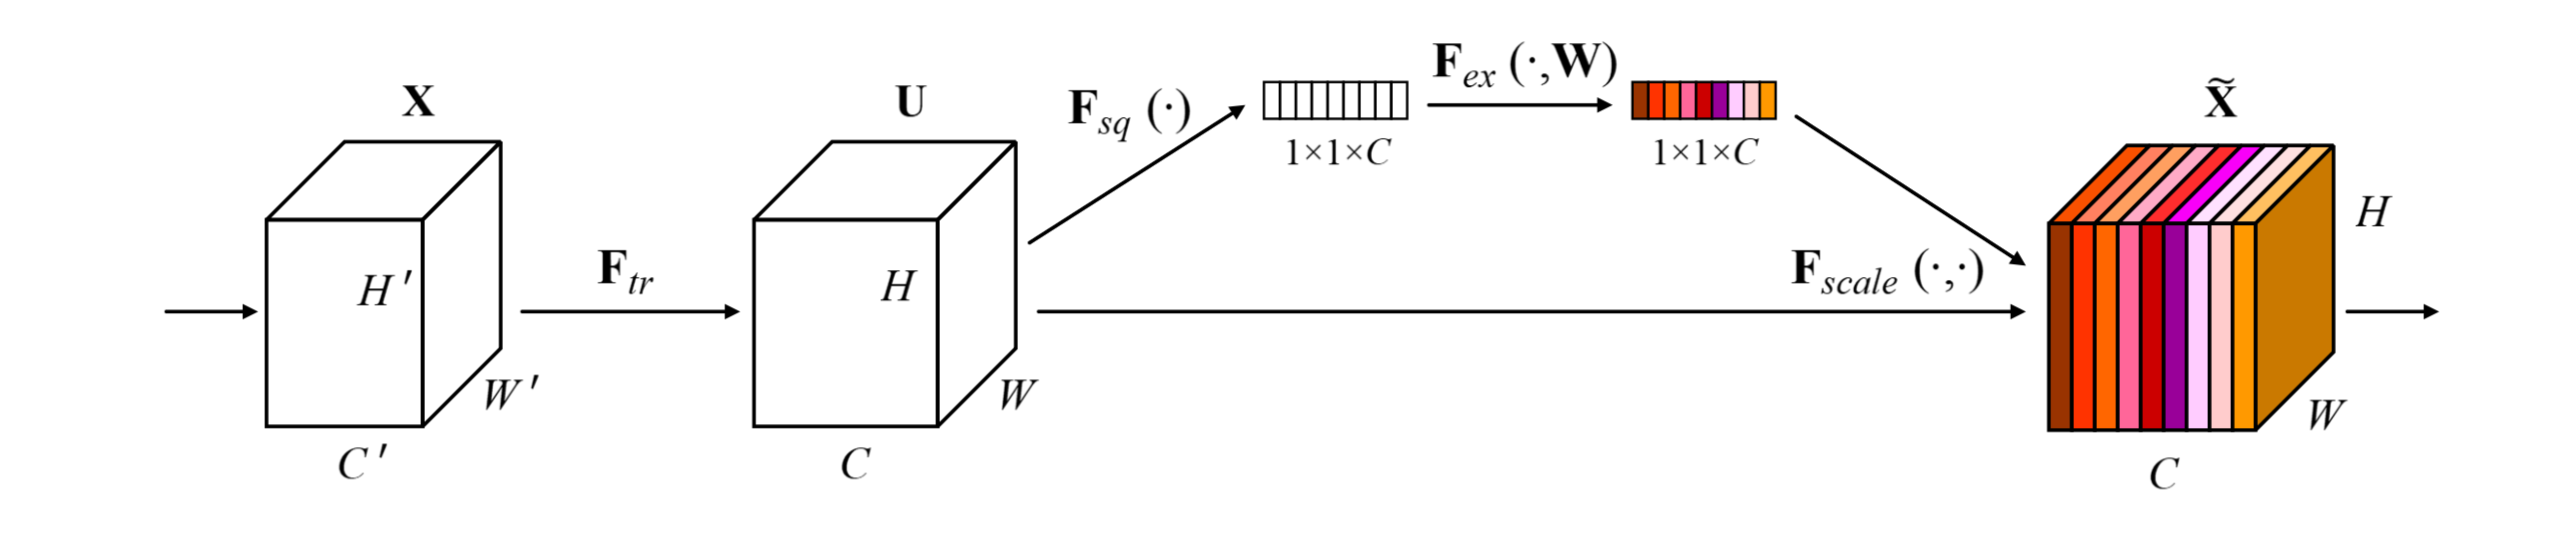
\includegraphics[width=\linewidth]{../img/implementation/estimator/se.png}
    \caption{\emph{Preactivation}}
\end{figure}
Our network differs is composed by $n$ ResNet blocks, a depth of $d$ and a channel incrementing factor of $2$. We select $n=1$ and $d=3$ with a starting channel size of $16$, we called this model architecture \emph{micro-resnet}. 

\begin{table}[H]
    \centering
    \begin{tabular}{|lc|}
        \hline
        & micro resnet \\
        \hline 
        & depth $=3$ \\ 
        \hline 
        & n $=1$ \\
        \hline
     &$3 \ x\ 3,\ 16 \ stride\ 1$ \\ 
     \hline
     &$2 \ x\ 2$ max-pool \\ 
     \hline
     & \\
     &$\begin{bmatrix}
      3\ x\ 3, & 16 \\
      3\ x \ 3, & 16 \\  
     \end{bmatrix}$ x 1 \\ 
     & \\
     \hline     
     & SE-module\\ 
     \hline     
     & \\
     &$\begin{bmatrix}
        3\ x \ 3, & 32 \\
        3\ x\ 3, & 32 \\  
       \end{bmatrix}$ x 1 \\\
       & \\ 
       \hline
       & SE-module\\ 
       \hline
       & \\
       &$\begin{bmatrix}
        3\ x \ 3, & 64 \\
        3 \ x \ 3, & 64 \\  
       \end{bmatrix}$ x 1 \\  
       & \\
       \hline     
       & SE-module\\ 
       \hline
       & average pool, $1$-d fc, softmax \\ 
       \hline

    \end{tabular}
    \caption{\emph{micro-resnet} architecture}
\end{table}

\todo[inline]{add model picture}
\subsubsection{Normalization}
Before feeding the data to the models, we need to make the patches height invariant. This must be done to correctly normalize different patches taken from different maps with different height scaling factor. We subtract the height of the map corresponding \emph{Krock}'s position from the patch to correctly center it. The following figure shows the normalization process on the patch with the square in the middle.
\begin{figure}[H]
    \begin{subfigure}[b]{0.5\textwidth}
        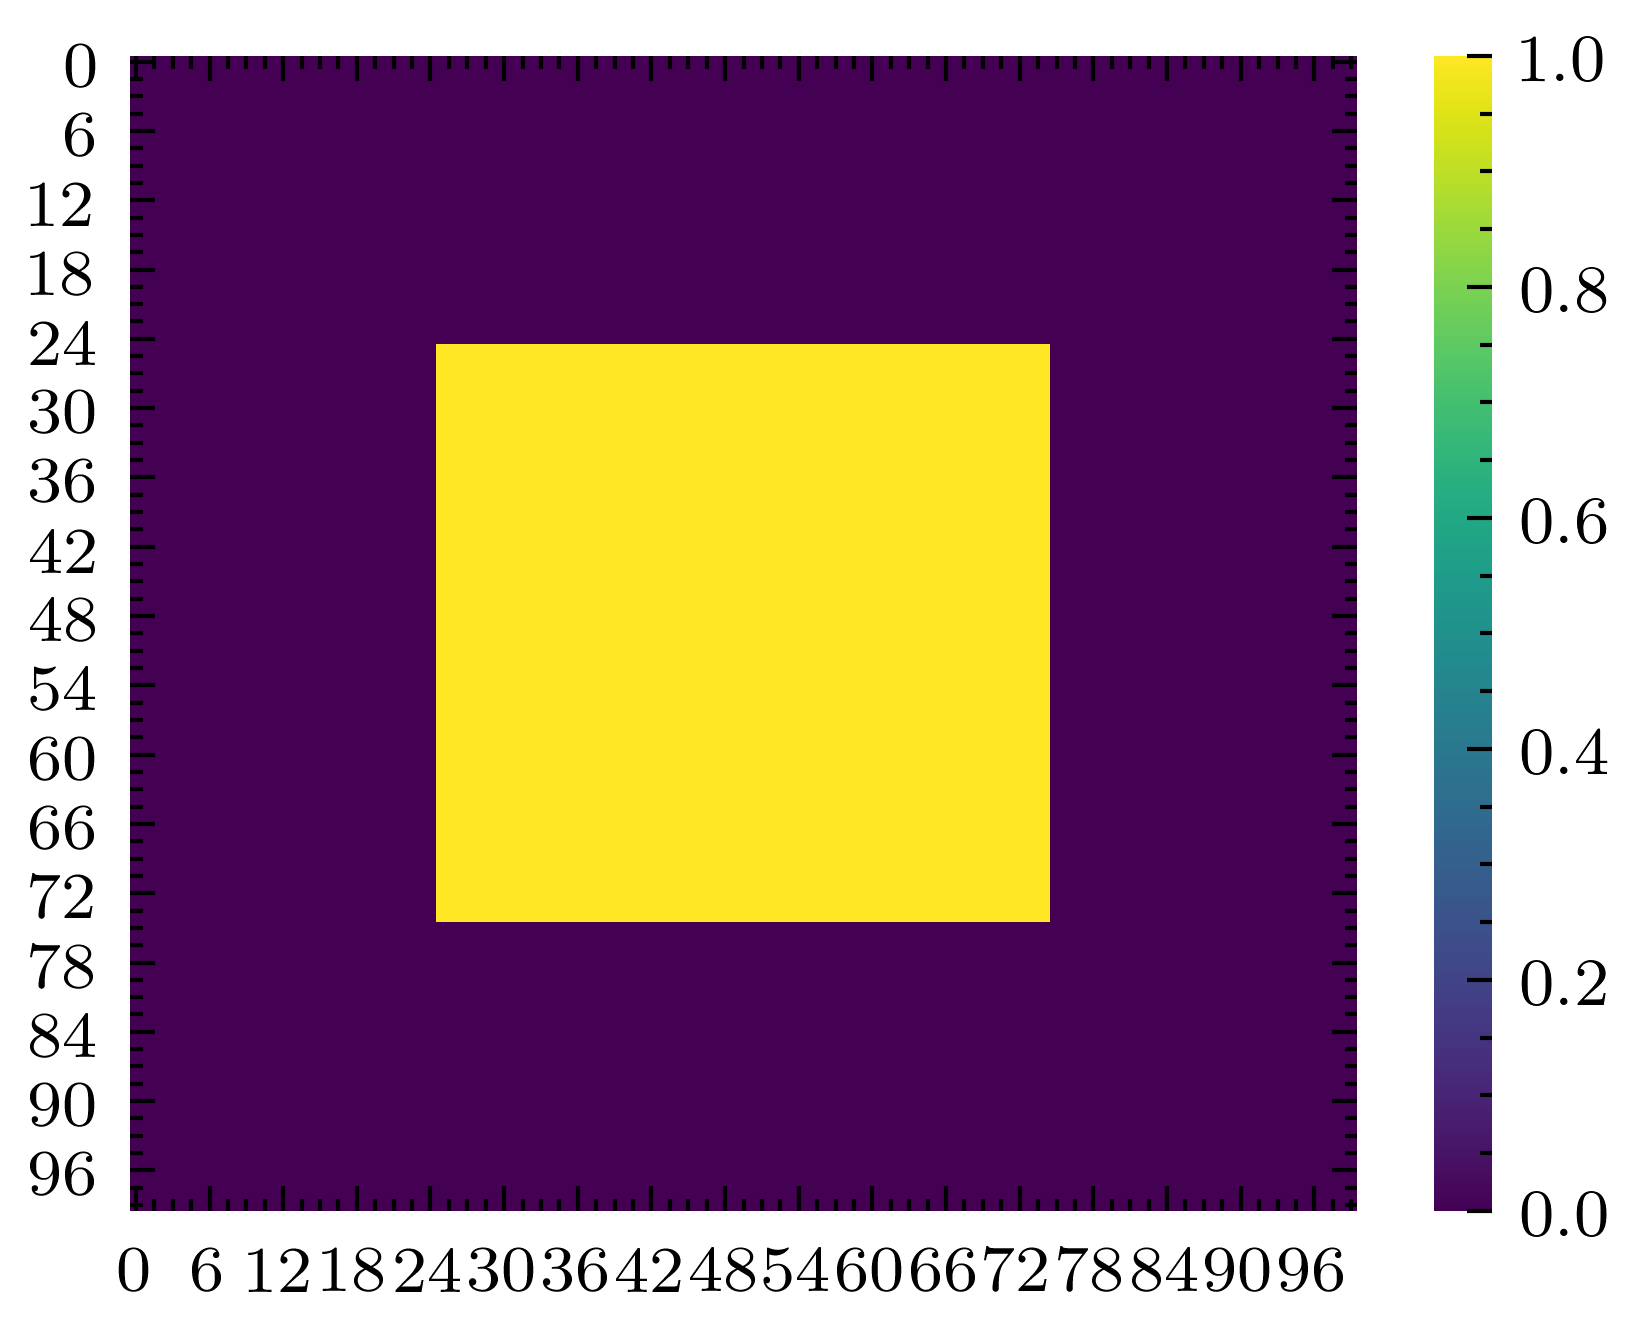
\includegraphics[width=\textwidth]{../img/data-aug/2d/square-middle.png}
        \caption{Input}
    \end{subfigure}
    \begin{subfigure}[b]{0.5\textwidth}
        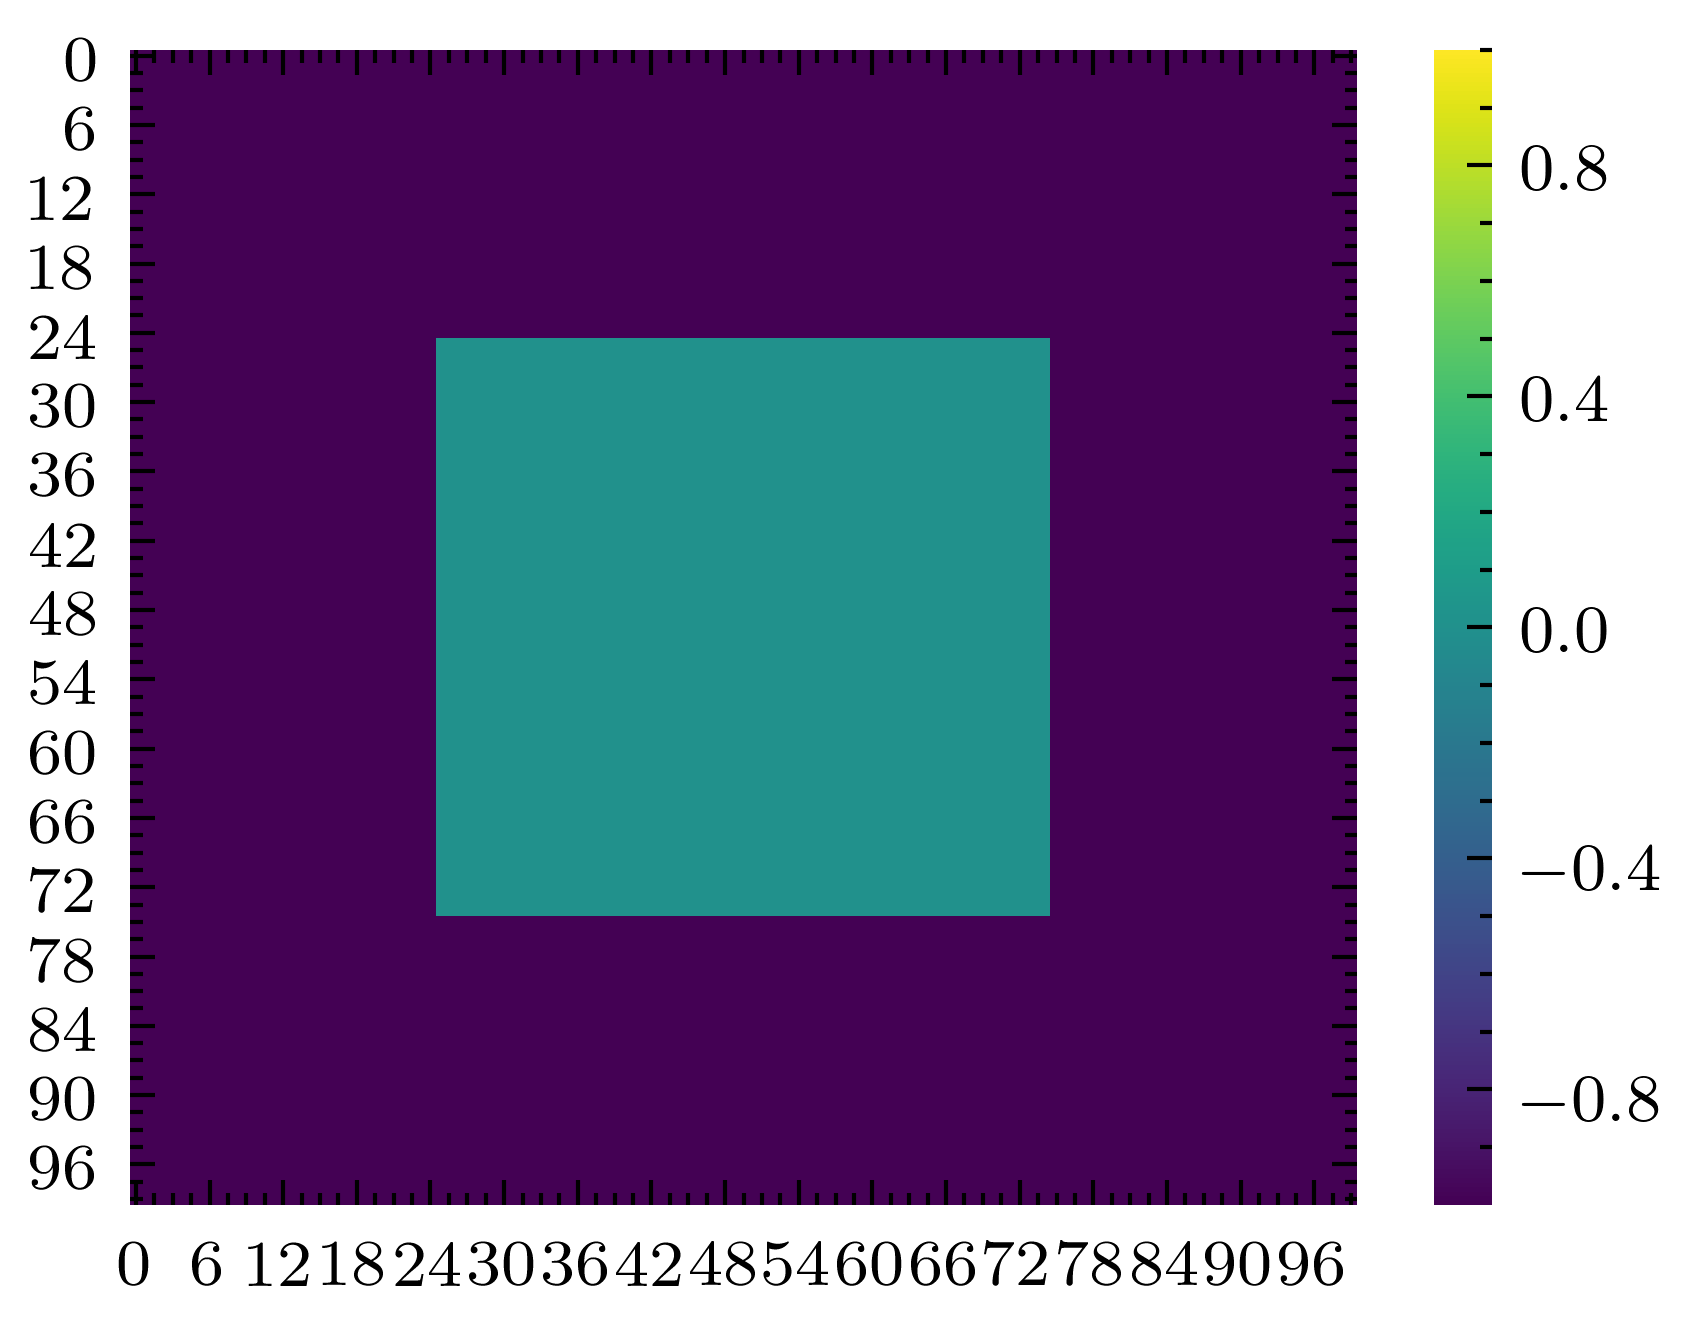
\includegraphics[width=\textwidth]{../img/data-aug/2d/square-middle-center.png}
        \caption{Height centered}
    \end{subfigure}  
    
          \begin{subfigure}[b]{0.5\textwidth}
        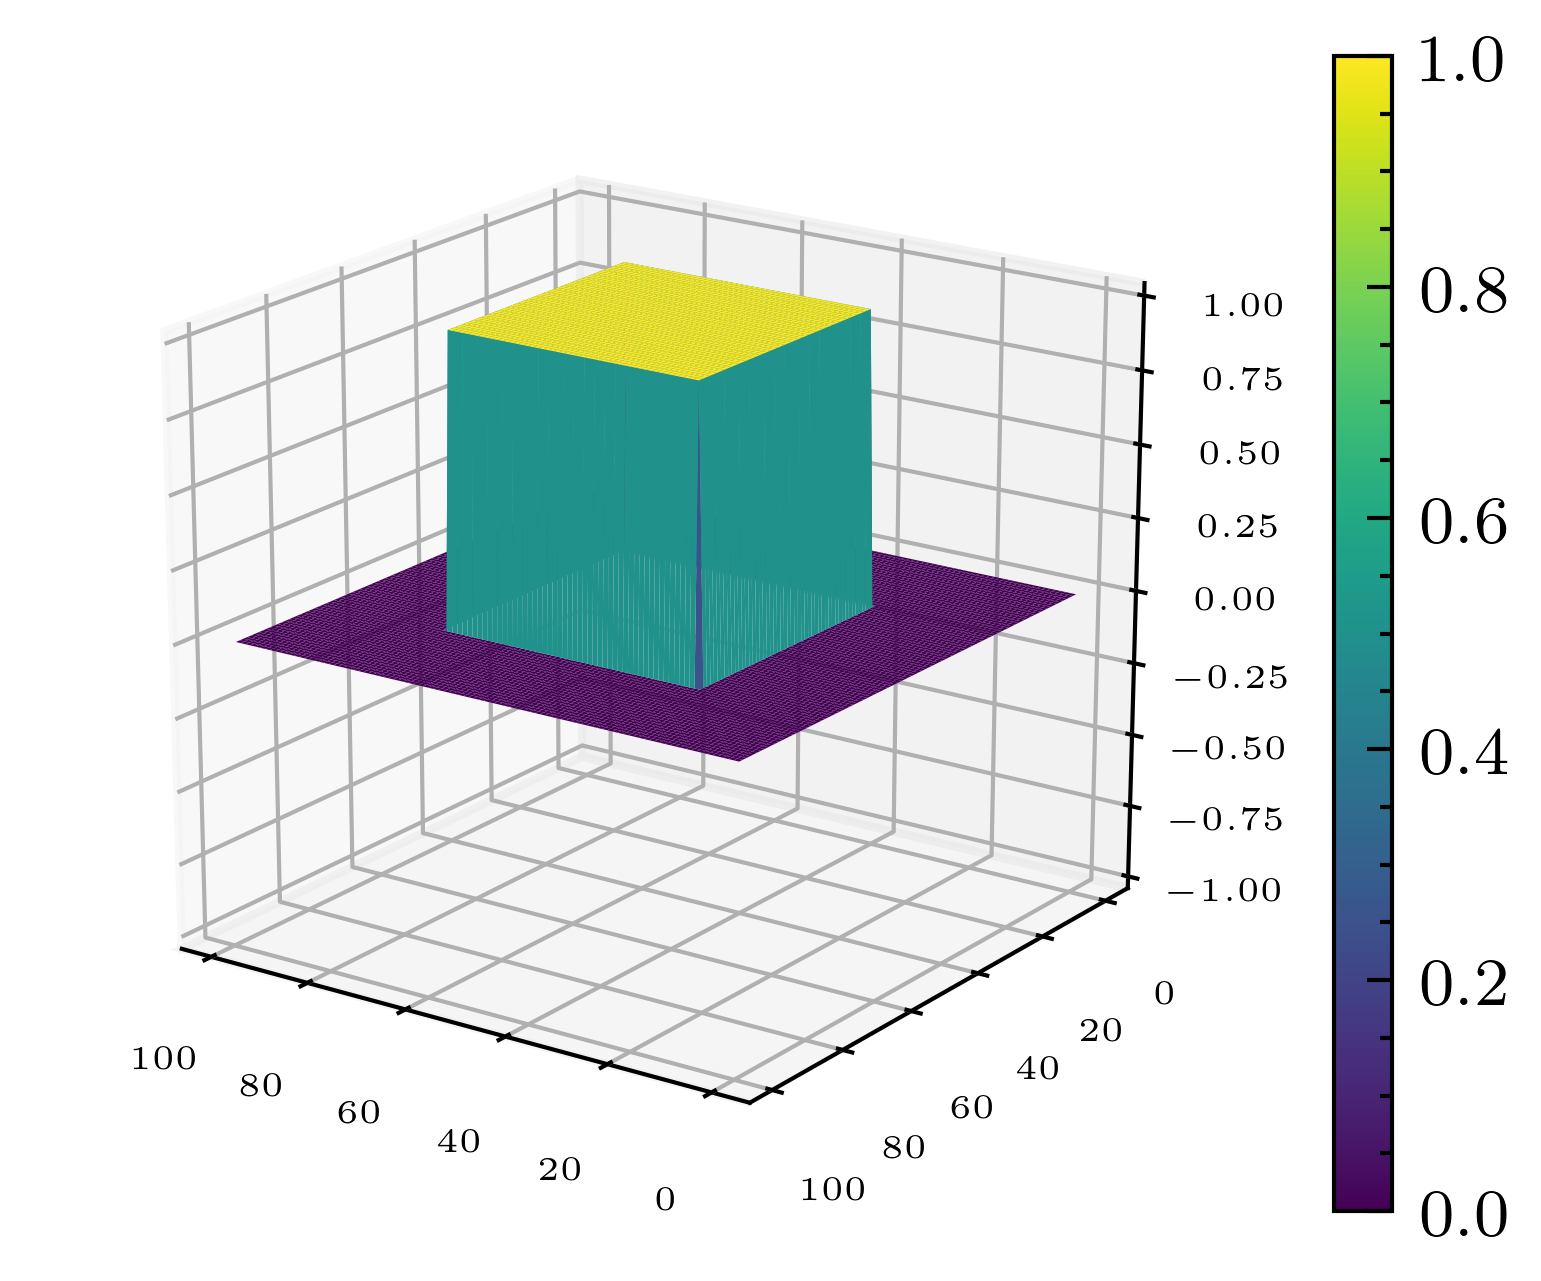
\includegraphics[width=\textwidth]{../img/data-aug/3d/square-middle.png}
        \caption{Input}
    \end{subfigure}
    \begin{subfigure}[b]{0.5\textwidth}
        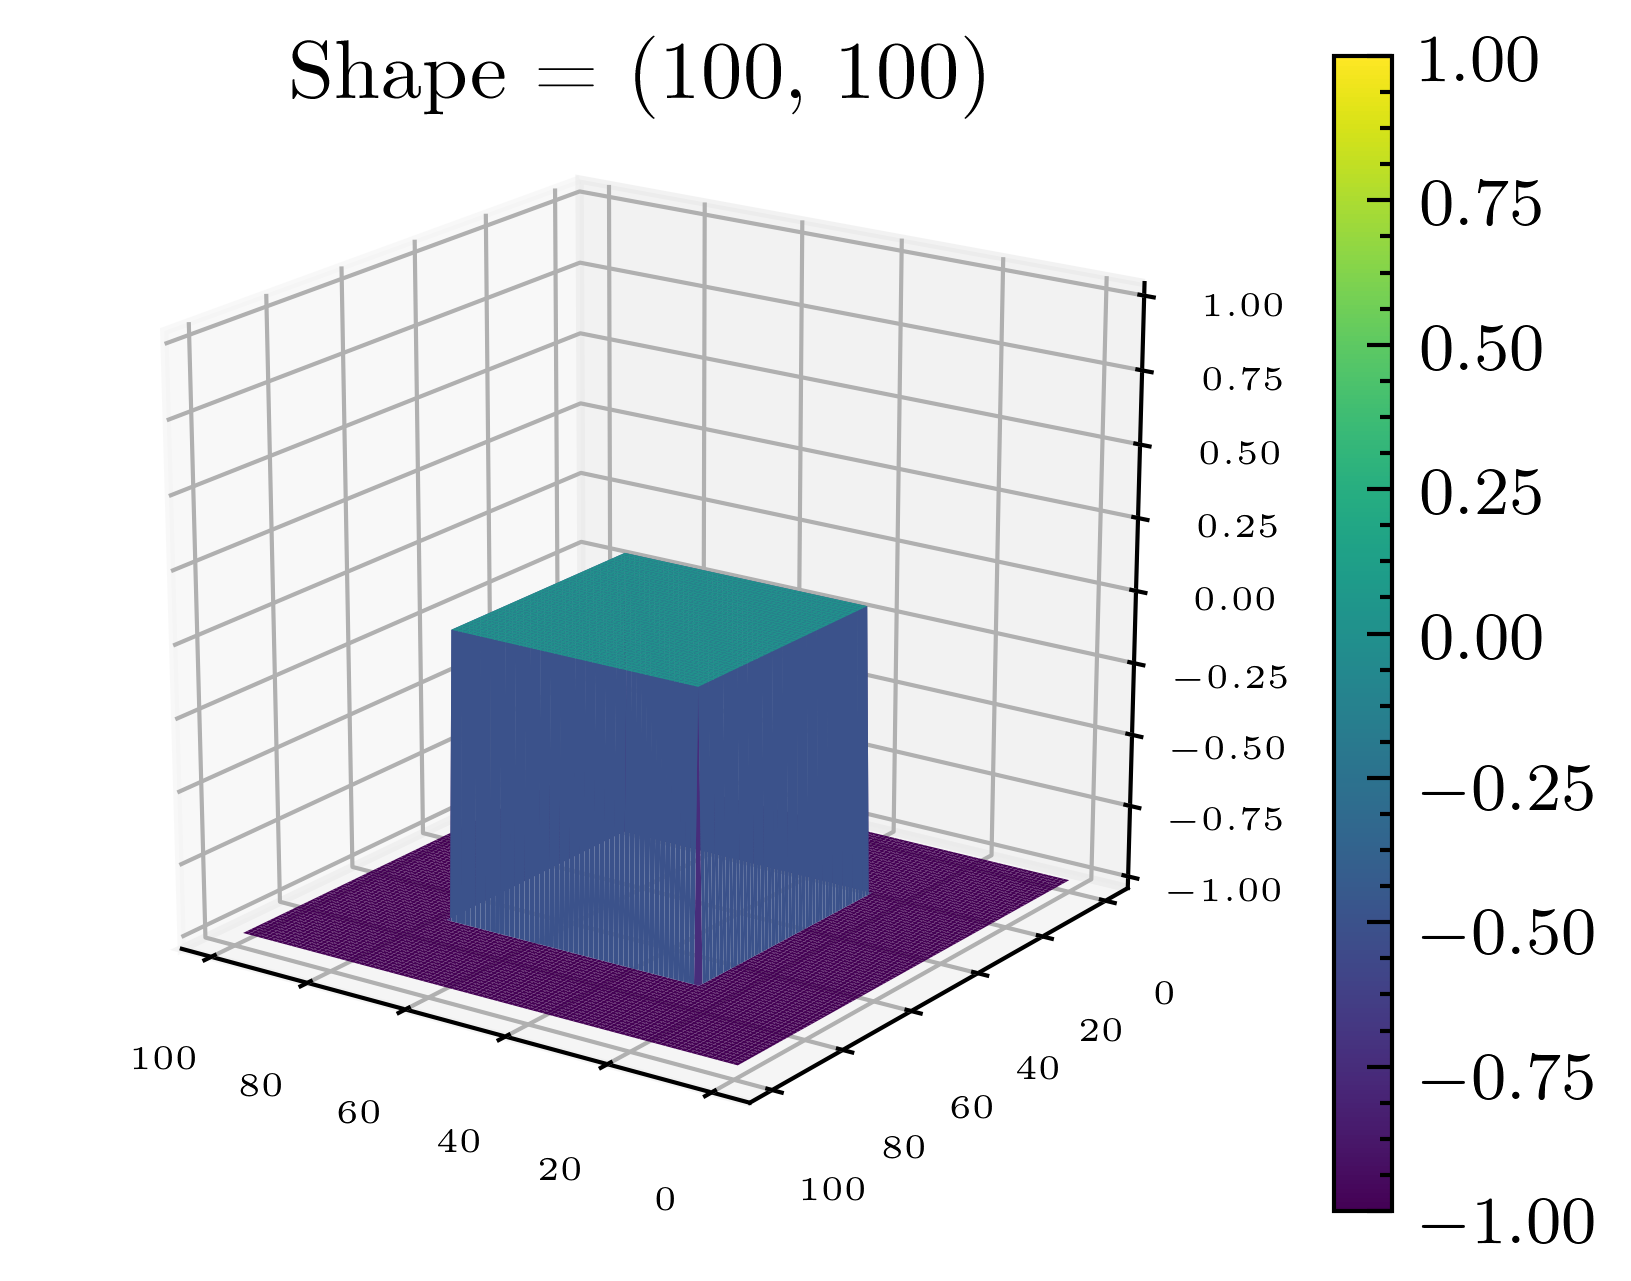
\includegraphics[width=\textwidth]{../img/data-aug/3d/square-middle-center.png}
        \caption{Height centered}
    \end{subfigure}  
\label{fig: center}
\caption{Normalization process}    
\end{figure}

\subsubsection{Data Augmentation}
Data augmentation is used to change the input of a model using different techniques to change it in order to produce more training examples. Since our inputs are heightmaps we cannot utilize the classic image manipulations such as shifts, flips, and zooms. Imagine that we have a patch with a wall in front of it, if we random rotate the image the wall may go in a position where the patch it is now traversable but its label is still not traversable, we have to be more creative. We decided to apply dropout, coarse dropout, and random simplex noise since they are traversability invariant. To illustrate those techniques we are going to use the following example patch of size $100x100$.
\begin{figure}[H]
    \begin{subfigure}[b]{0.5\textwidth}
        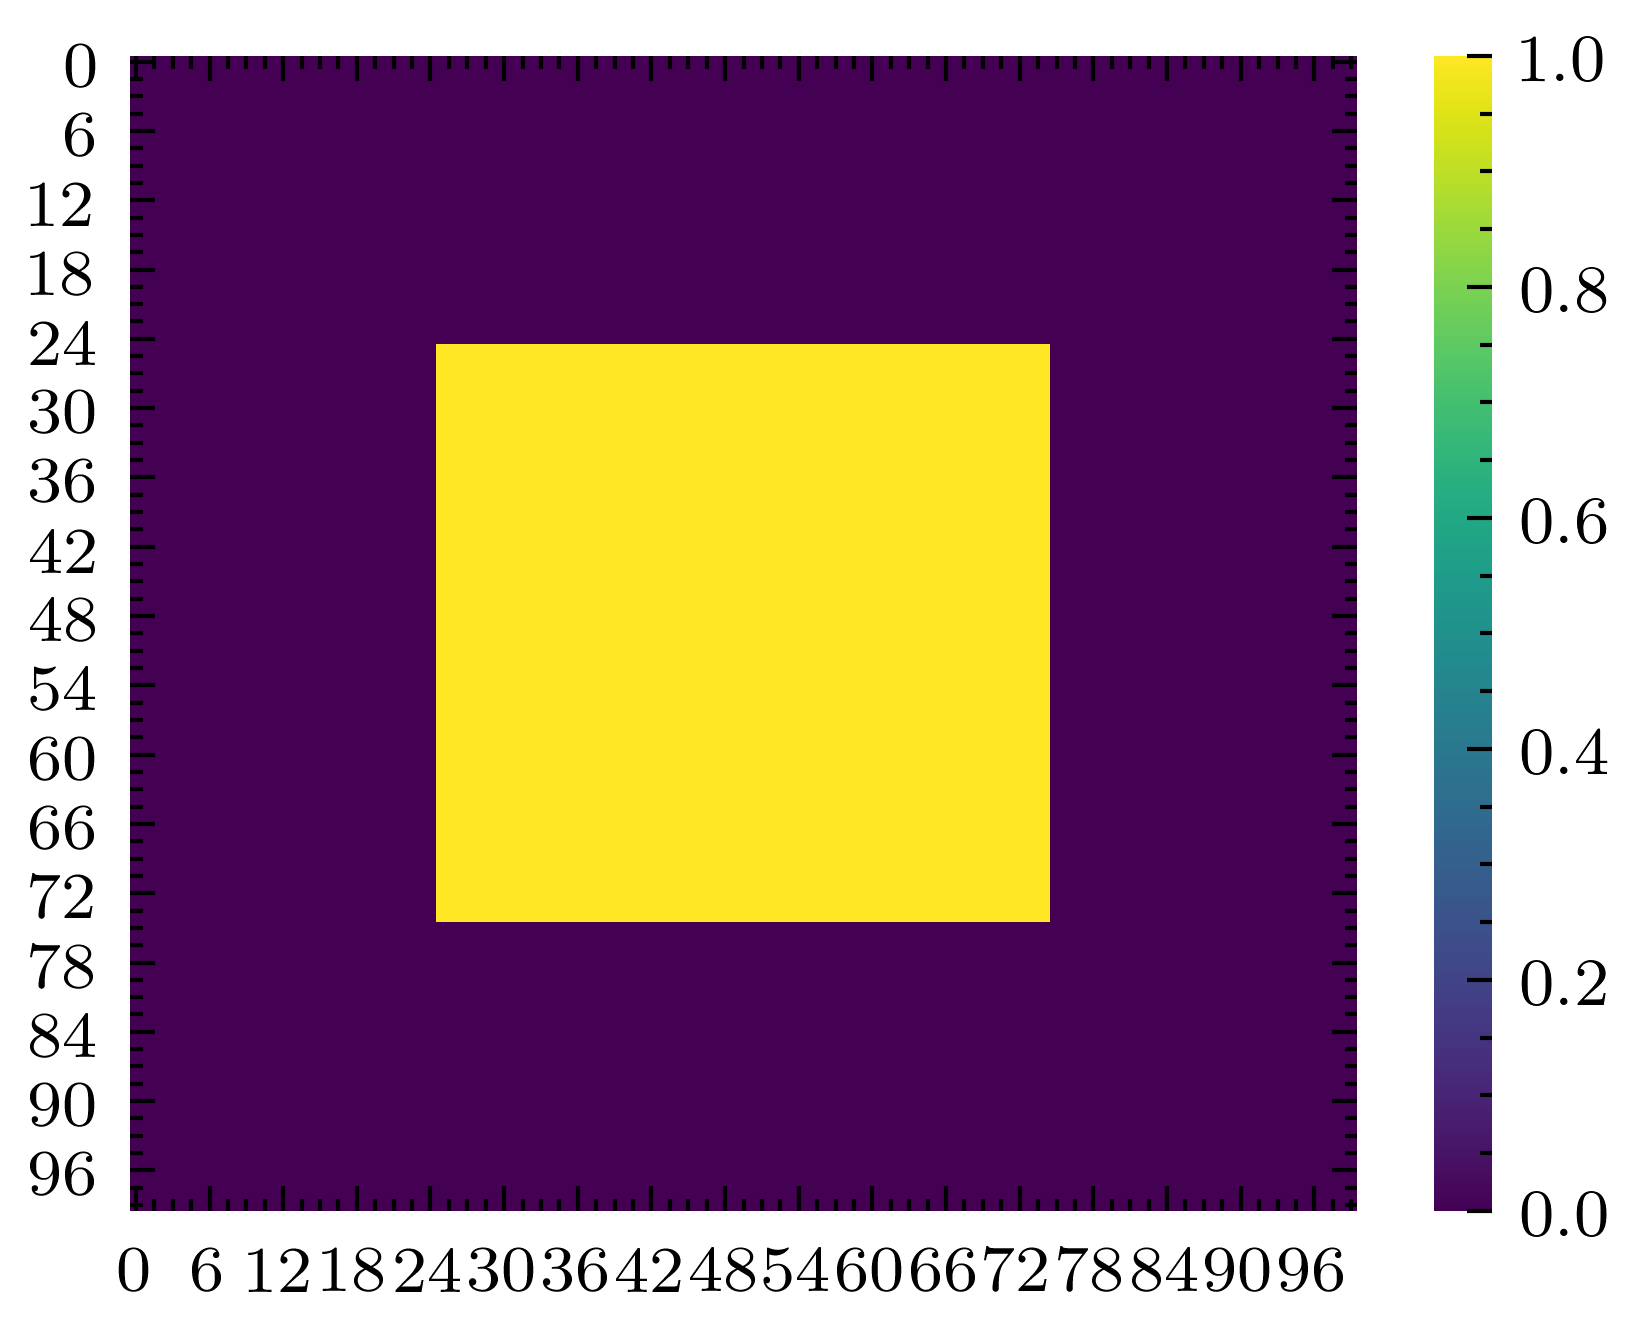
\includegraphics[width=\textwidth]{../img/data-aug/2d/square-middle.png}
    \end{subfigure}
    \begin{subfigure}[b]{0.5\textwidth}
        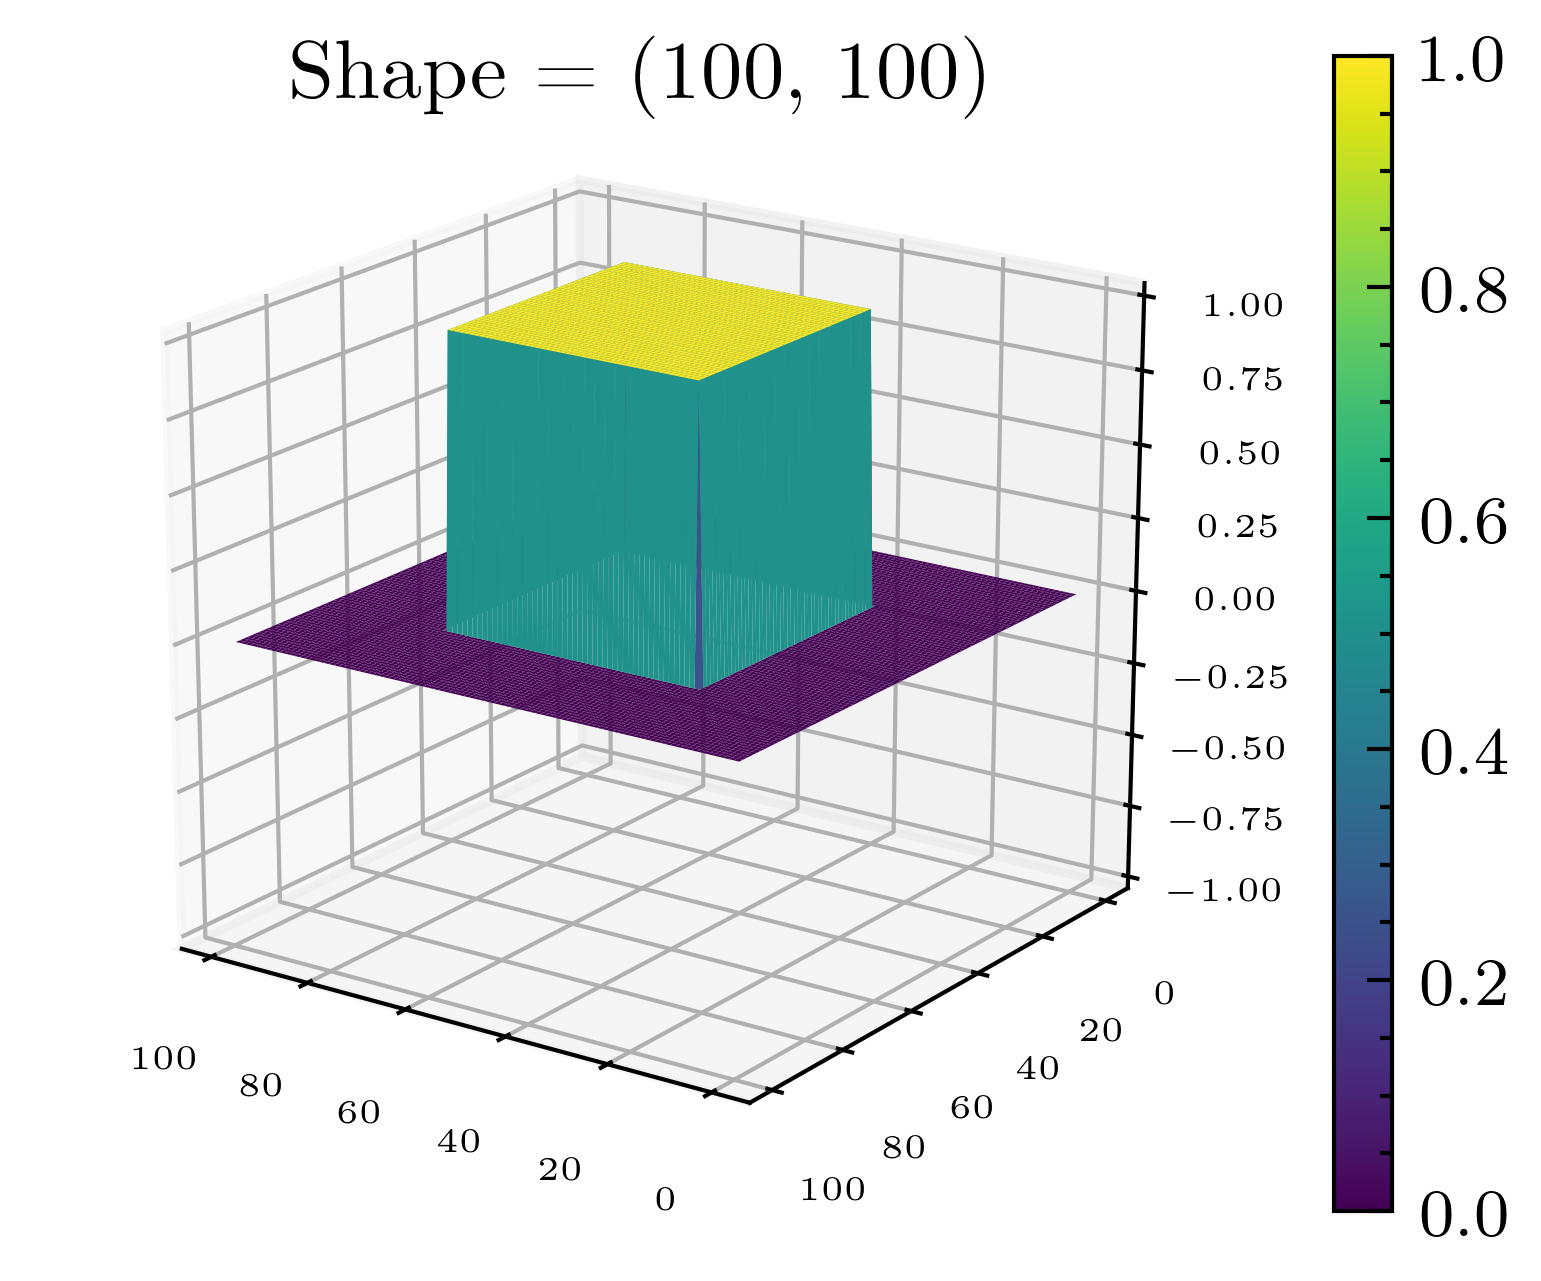
\includegraphics[width=\textwidth]{../img/data-aug/square-middle.png}
    \end{subfigure}    
\label{fig: square-patch}
\caption{A patch with a square in the middle}    
\end{figure}
\paragraph{Dropout} is a technique to randomly set some pixels to zero, in our case we flat some random pixel in the patch. 
\paragraph{Coarse Dropout} similar to dropout, it sets to zero random regions of pixels.
\paragraph{Simplex Noise} is a form of Perlin noise that is mostly used in ground generation. Our idea is to add some noise to make the network generalize better since lots of training maps have only obstacles in flat ground. Since it is computationally expensive, we randomly fist apply the noise to five hundred images with only zeros. Then, we randomly scaled them and add to the input image.
\begin{figure}[H]
    \centering

        \begin{subfigure}[b]{0.45\textwidth}
            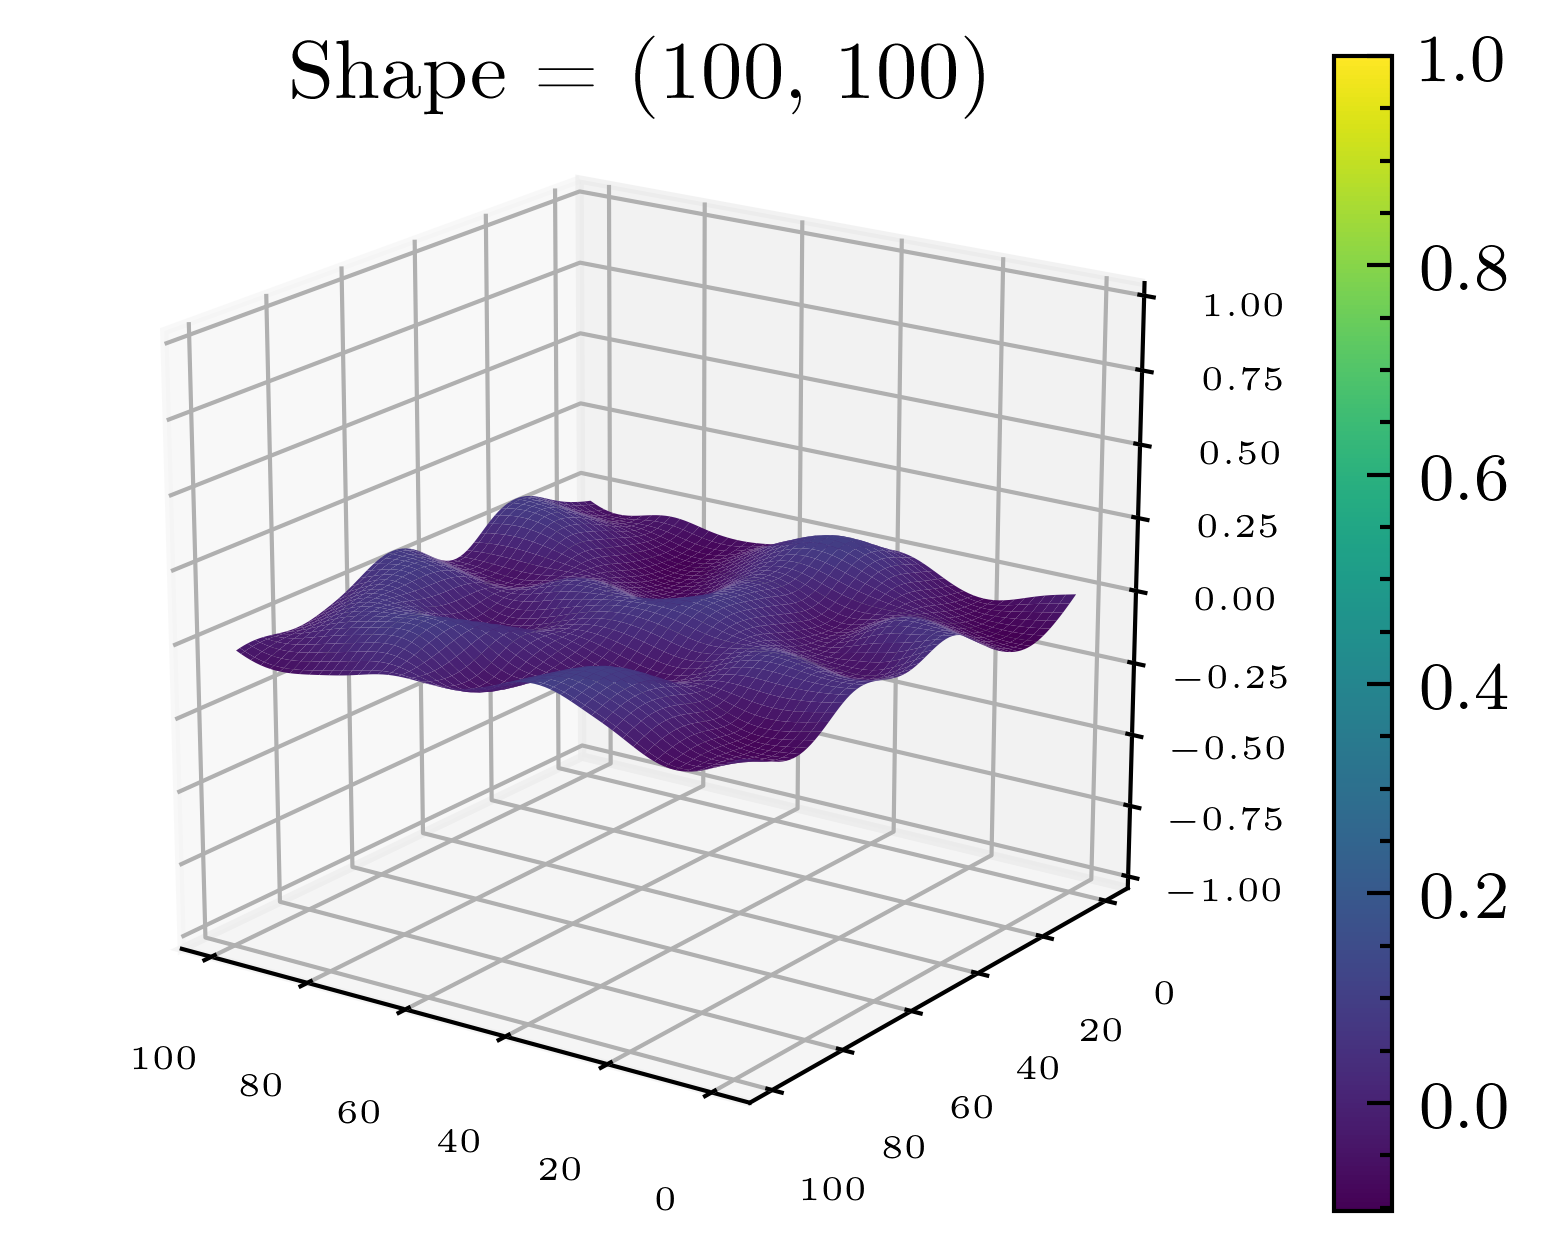
\includegraphics[width=\textwidth]{../img/data-aug/3d/simplex1.png}
            \caption{Features size = 10}
        \end{subfigure}
        \begin{subfigure}[b]{0.45\linewidth}
            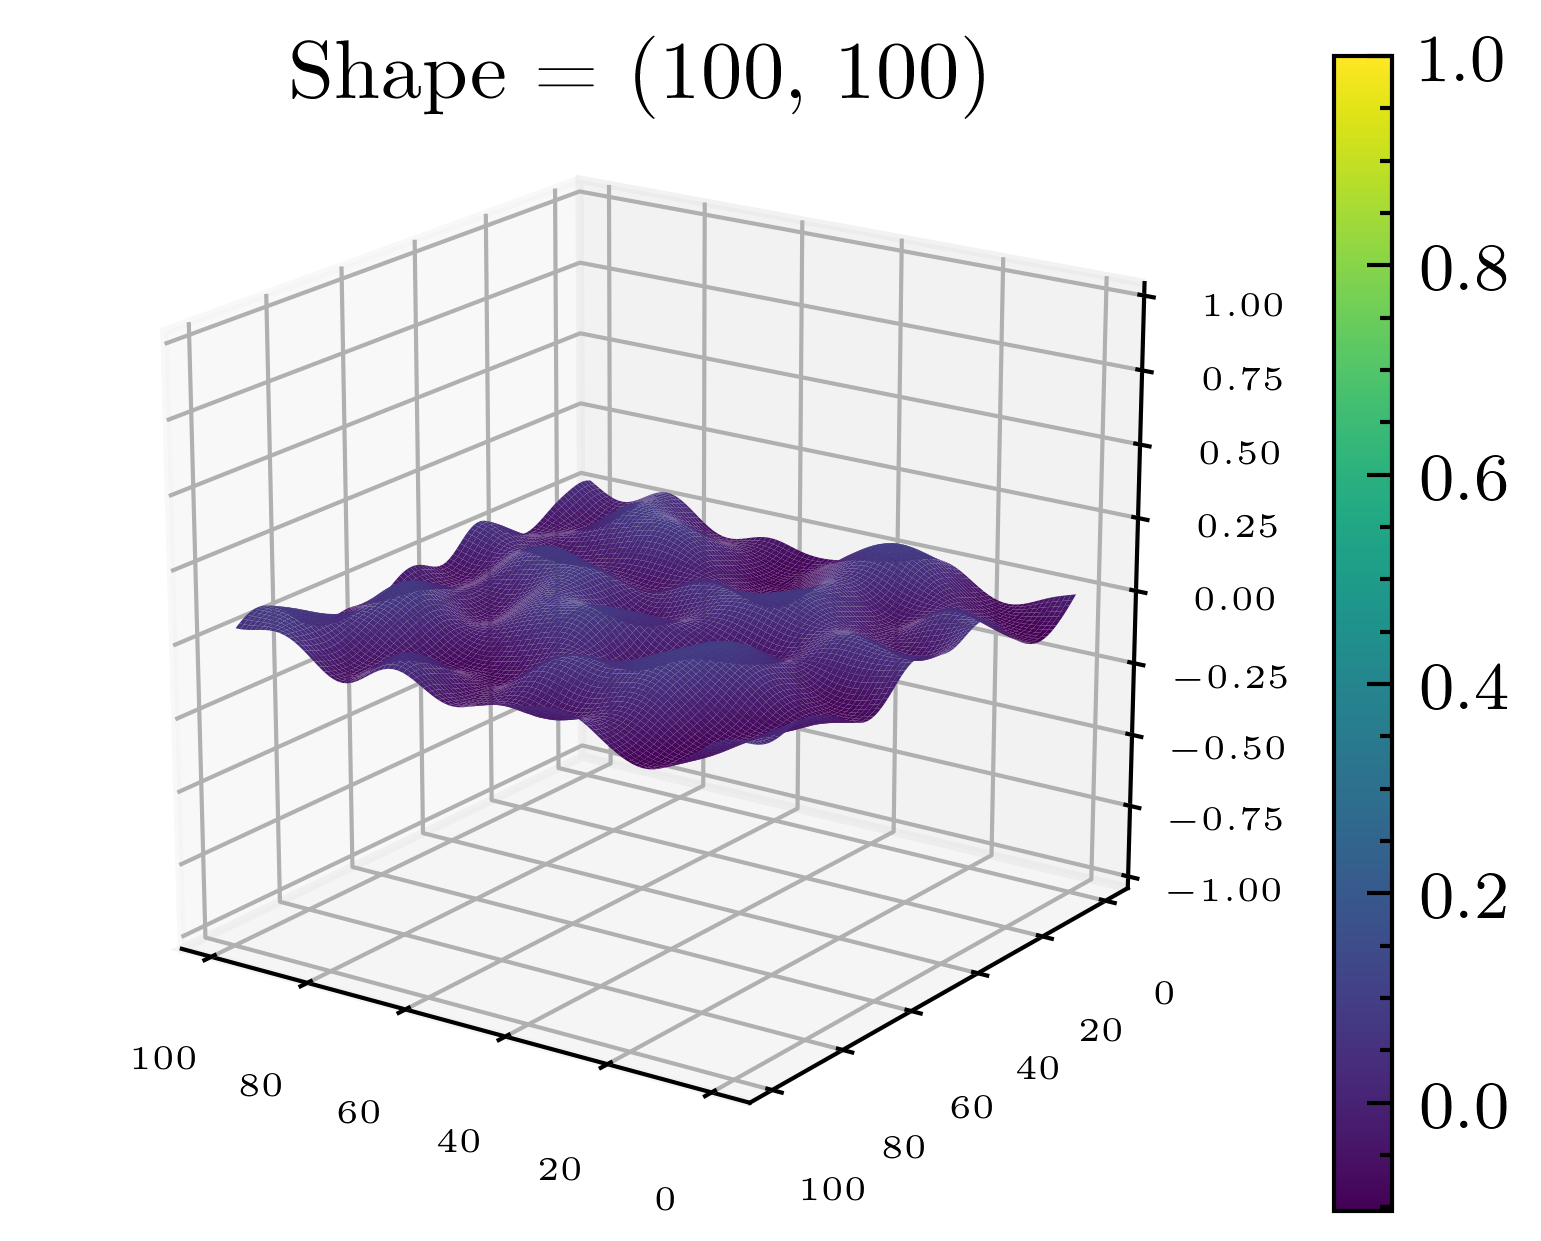
\includegraphics[width=\textwidth]{../img/data-aug/3d/simplex2.png}
            \caption{Data-aug}
            \end{subfigure}    
          \begin{subfigure}[b]{0.45\textwidth}
            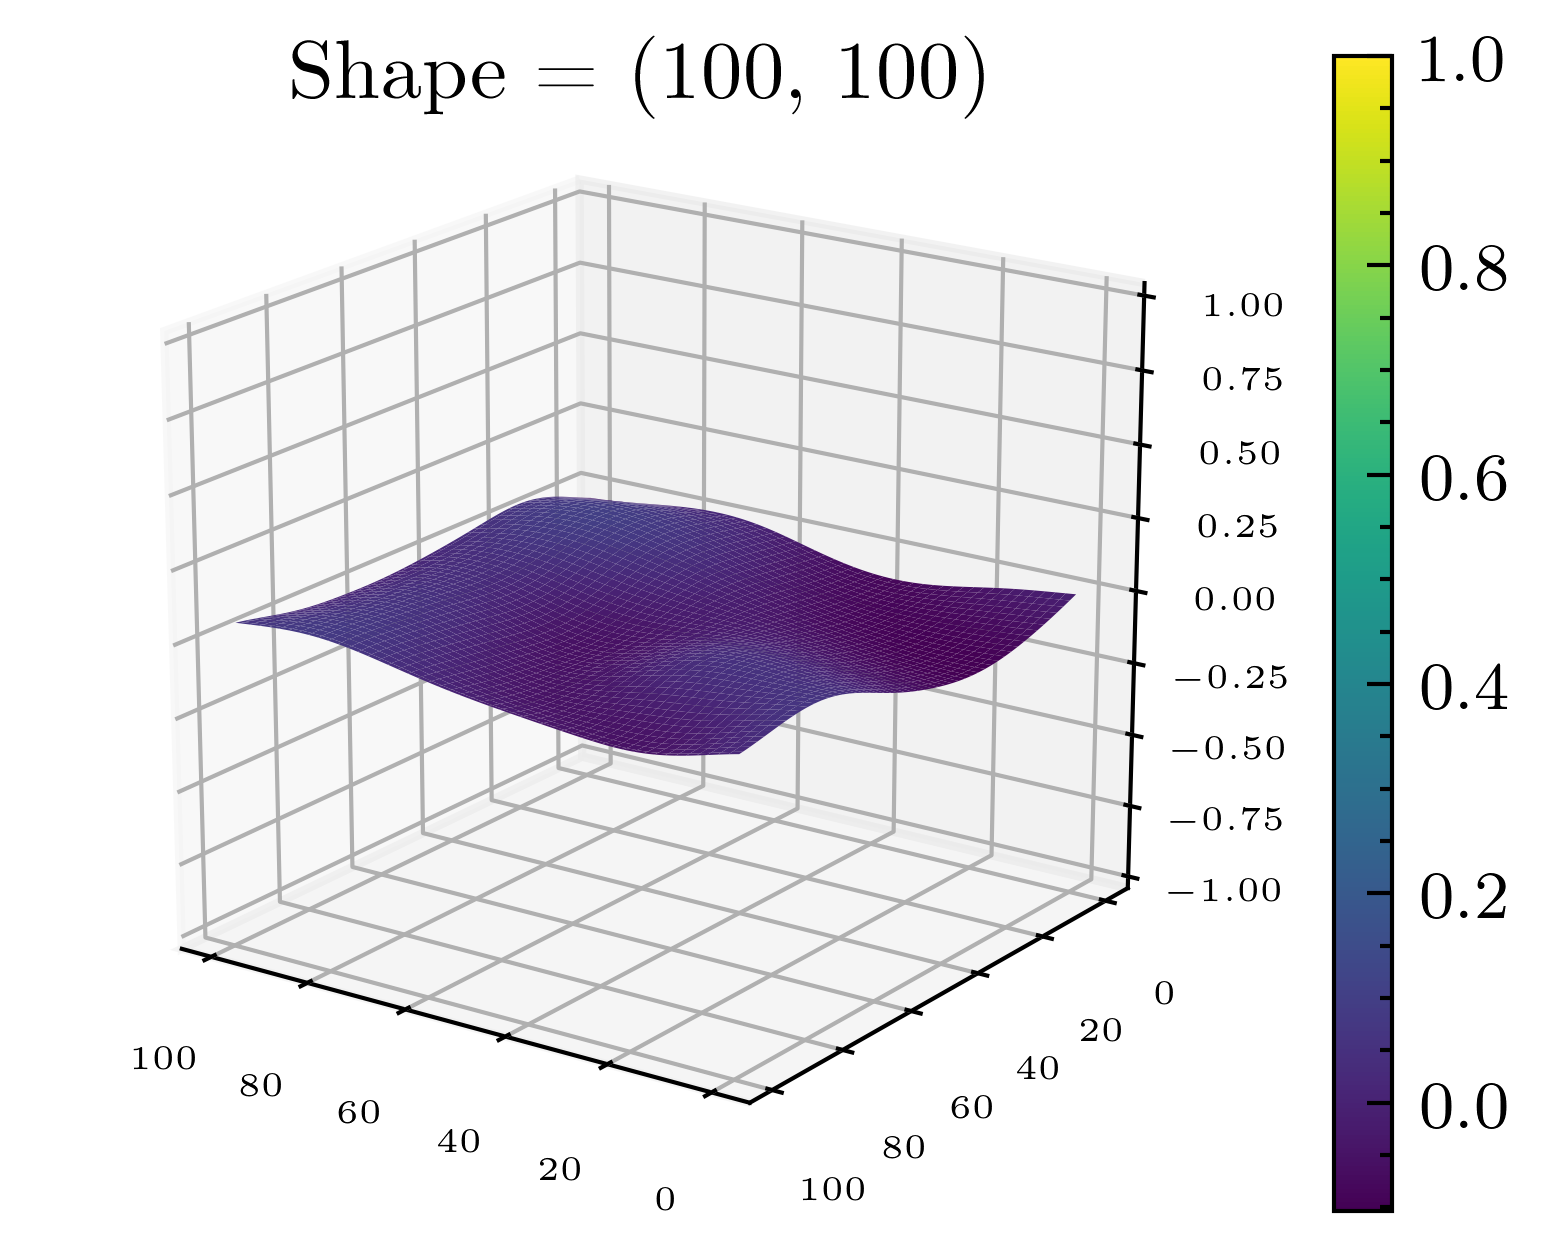
\includegraphics[width=\textwidth]{../img/data-aug/3d/simplex3.png}
            \caption{Features size = 30}
        \end{subfigure}    
        \begin{subfigure}[b]{0.45\textwidth}
            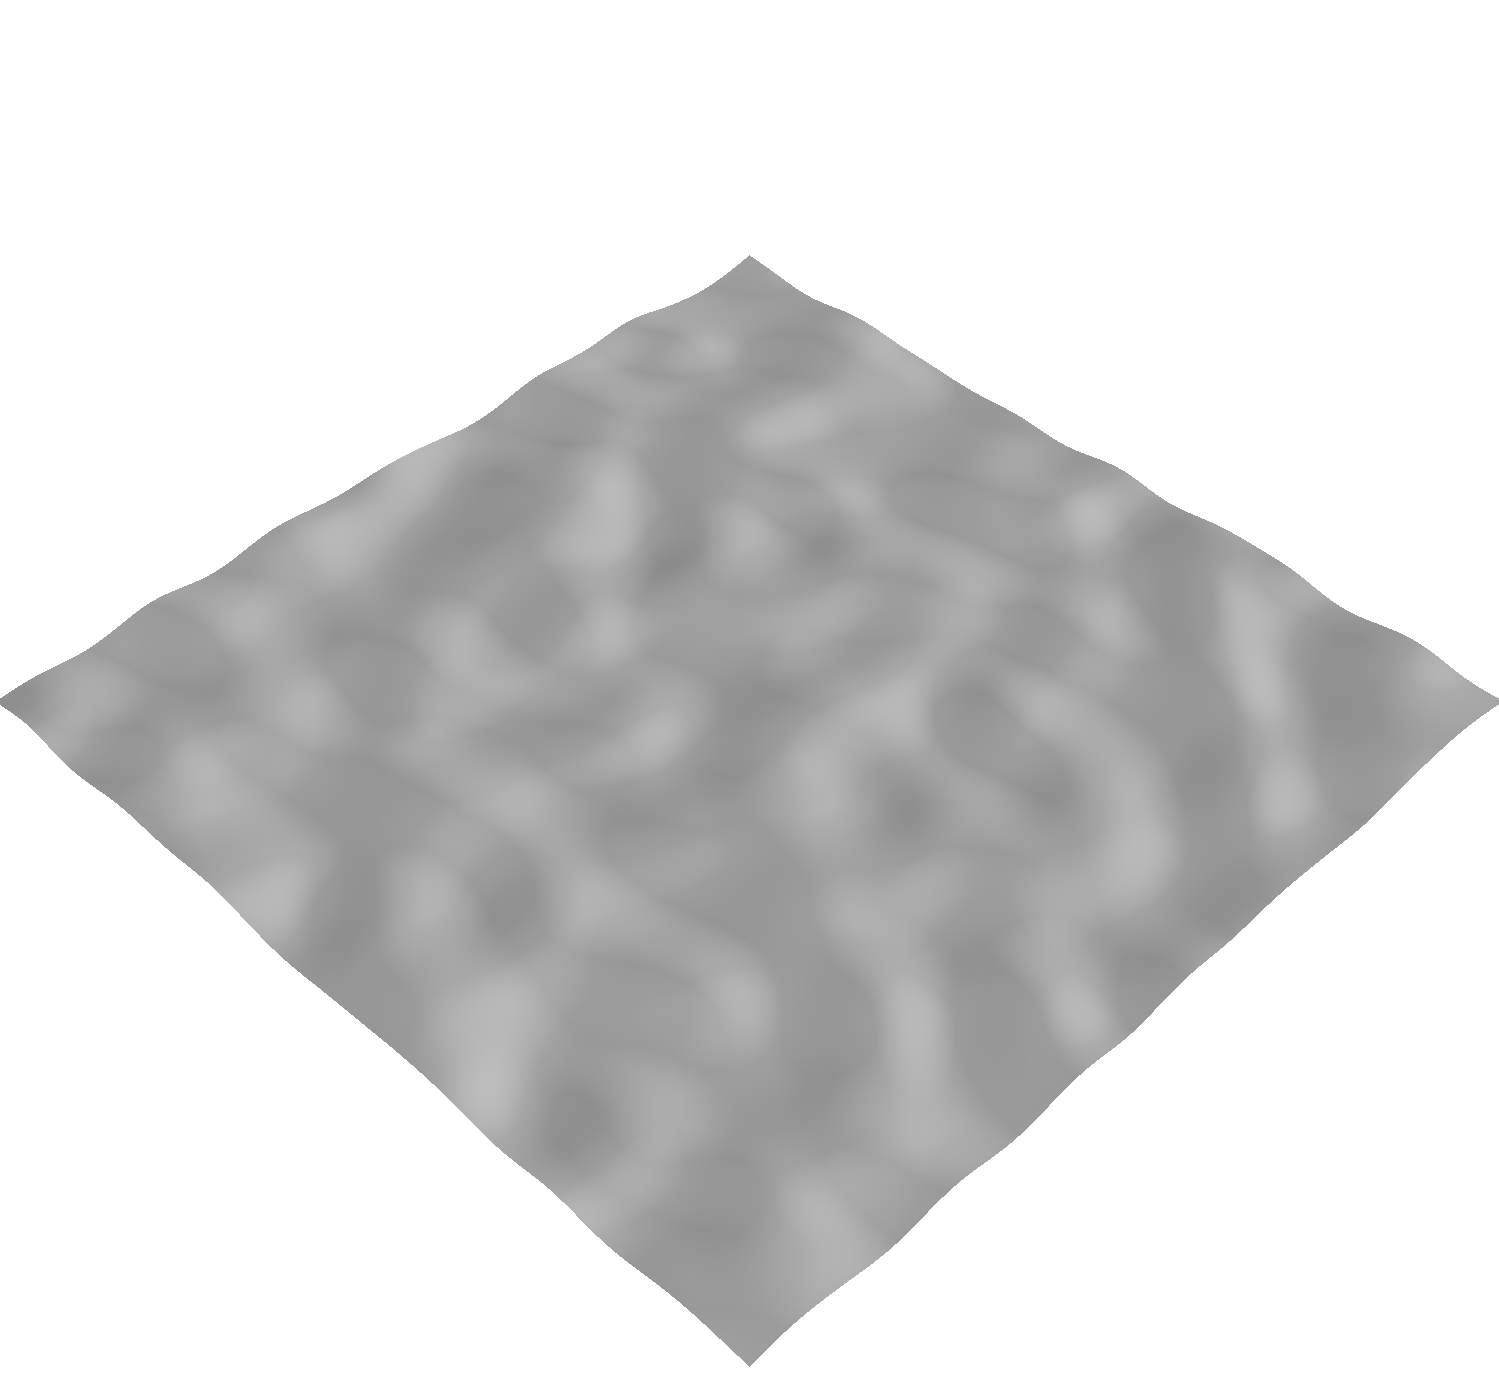
\includegraphics[width=\textwidth]{../img/data-aug/3d/simplex4.png}
            \caption{Features size = 40}
        \end{subfigure}    
    \label{fig: simplex-noise}
    \caption{Simplex Noise on flat ground}    
\end{figure}

The following images show the tree data augmentation techniques used applied the input image.
\begin{figure}[H]
    \centering
        \begin{subfigure}[b]{0.45\textwidth}
            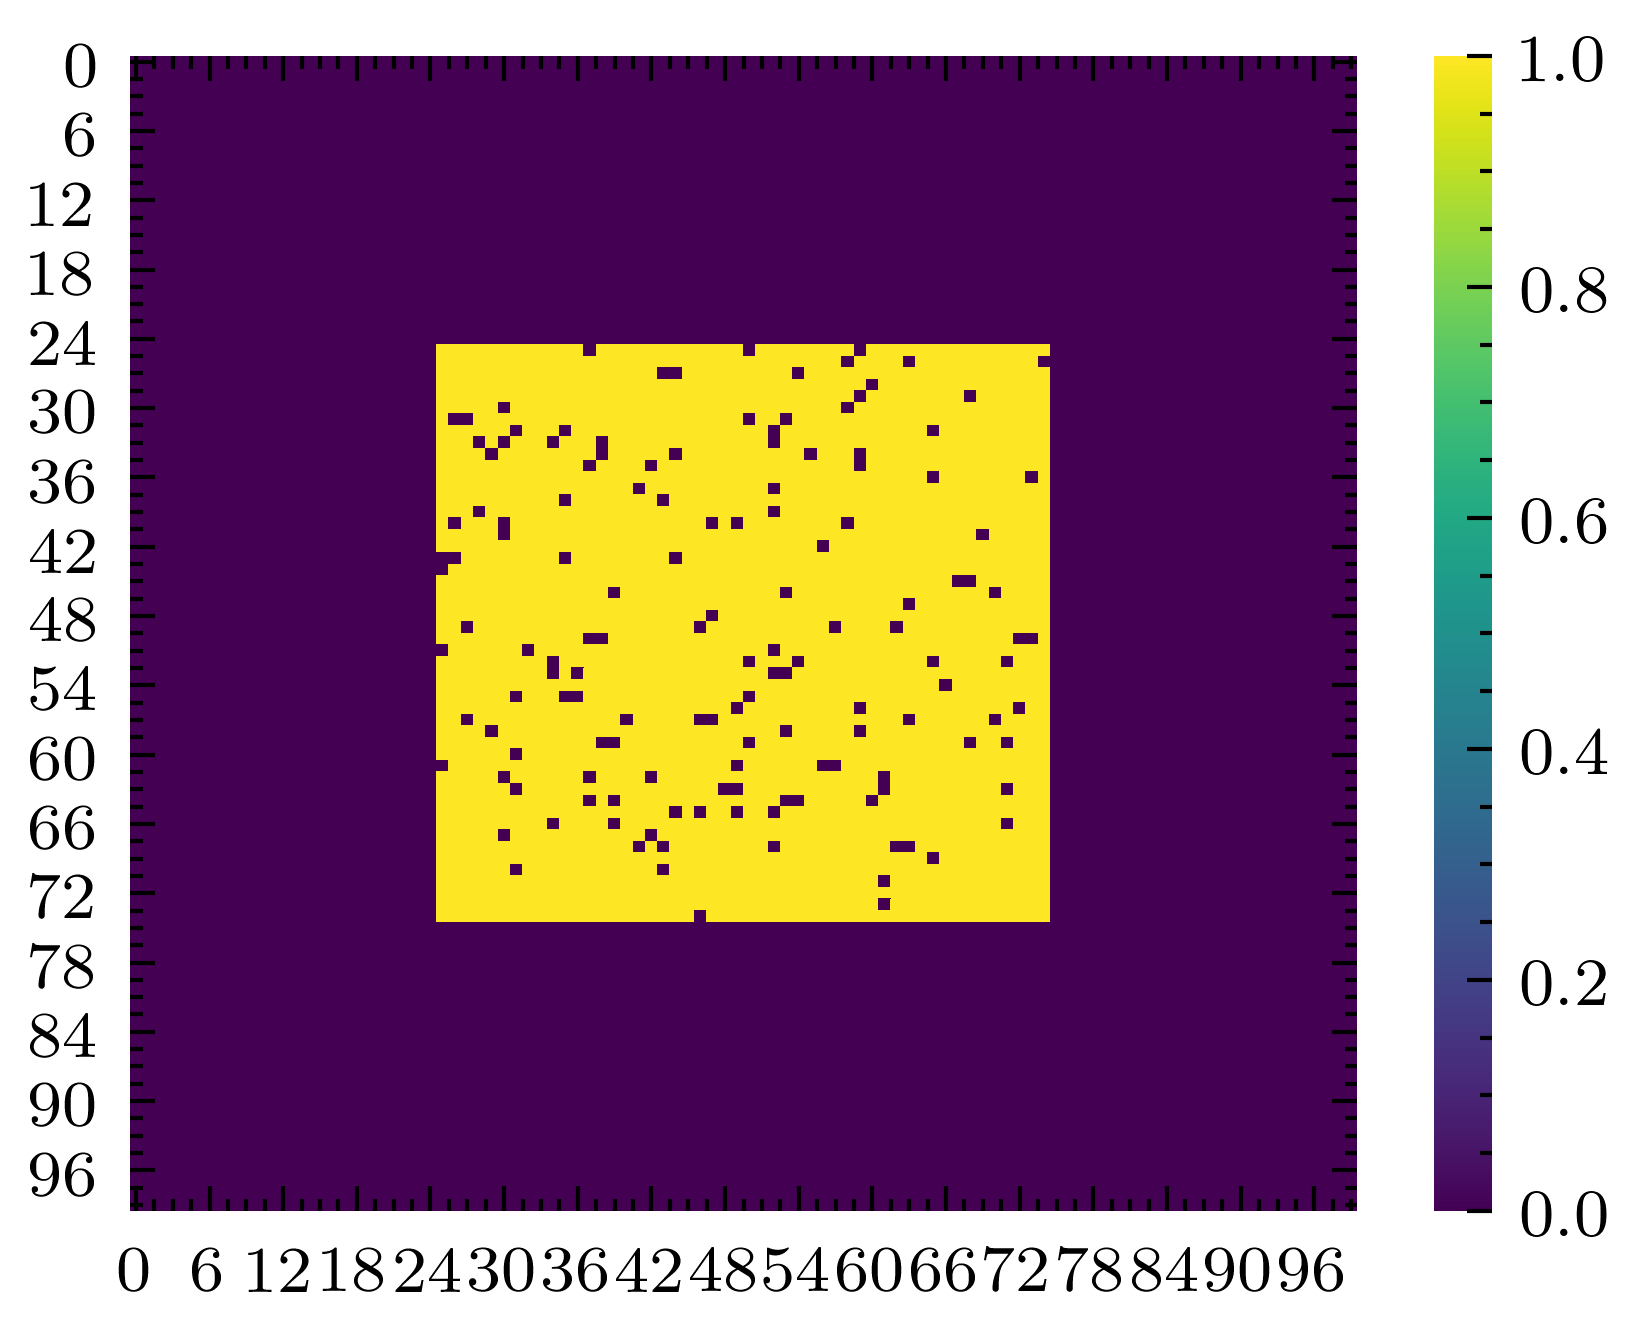
\includegraphics[width=\textwidth]{../img/data-aug/2d/center-dropout.png}
            \caption{Dropout}
        \end{subfigure}
        \begin{subfigure}[b]{0.45\linewidth}
            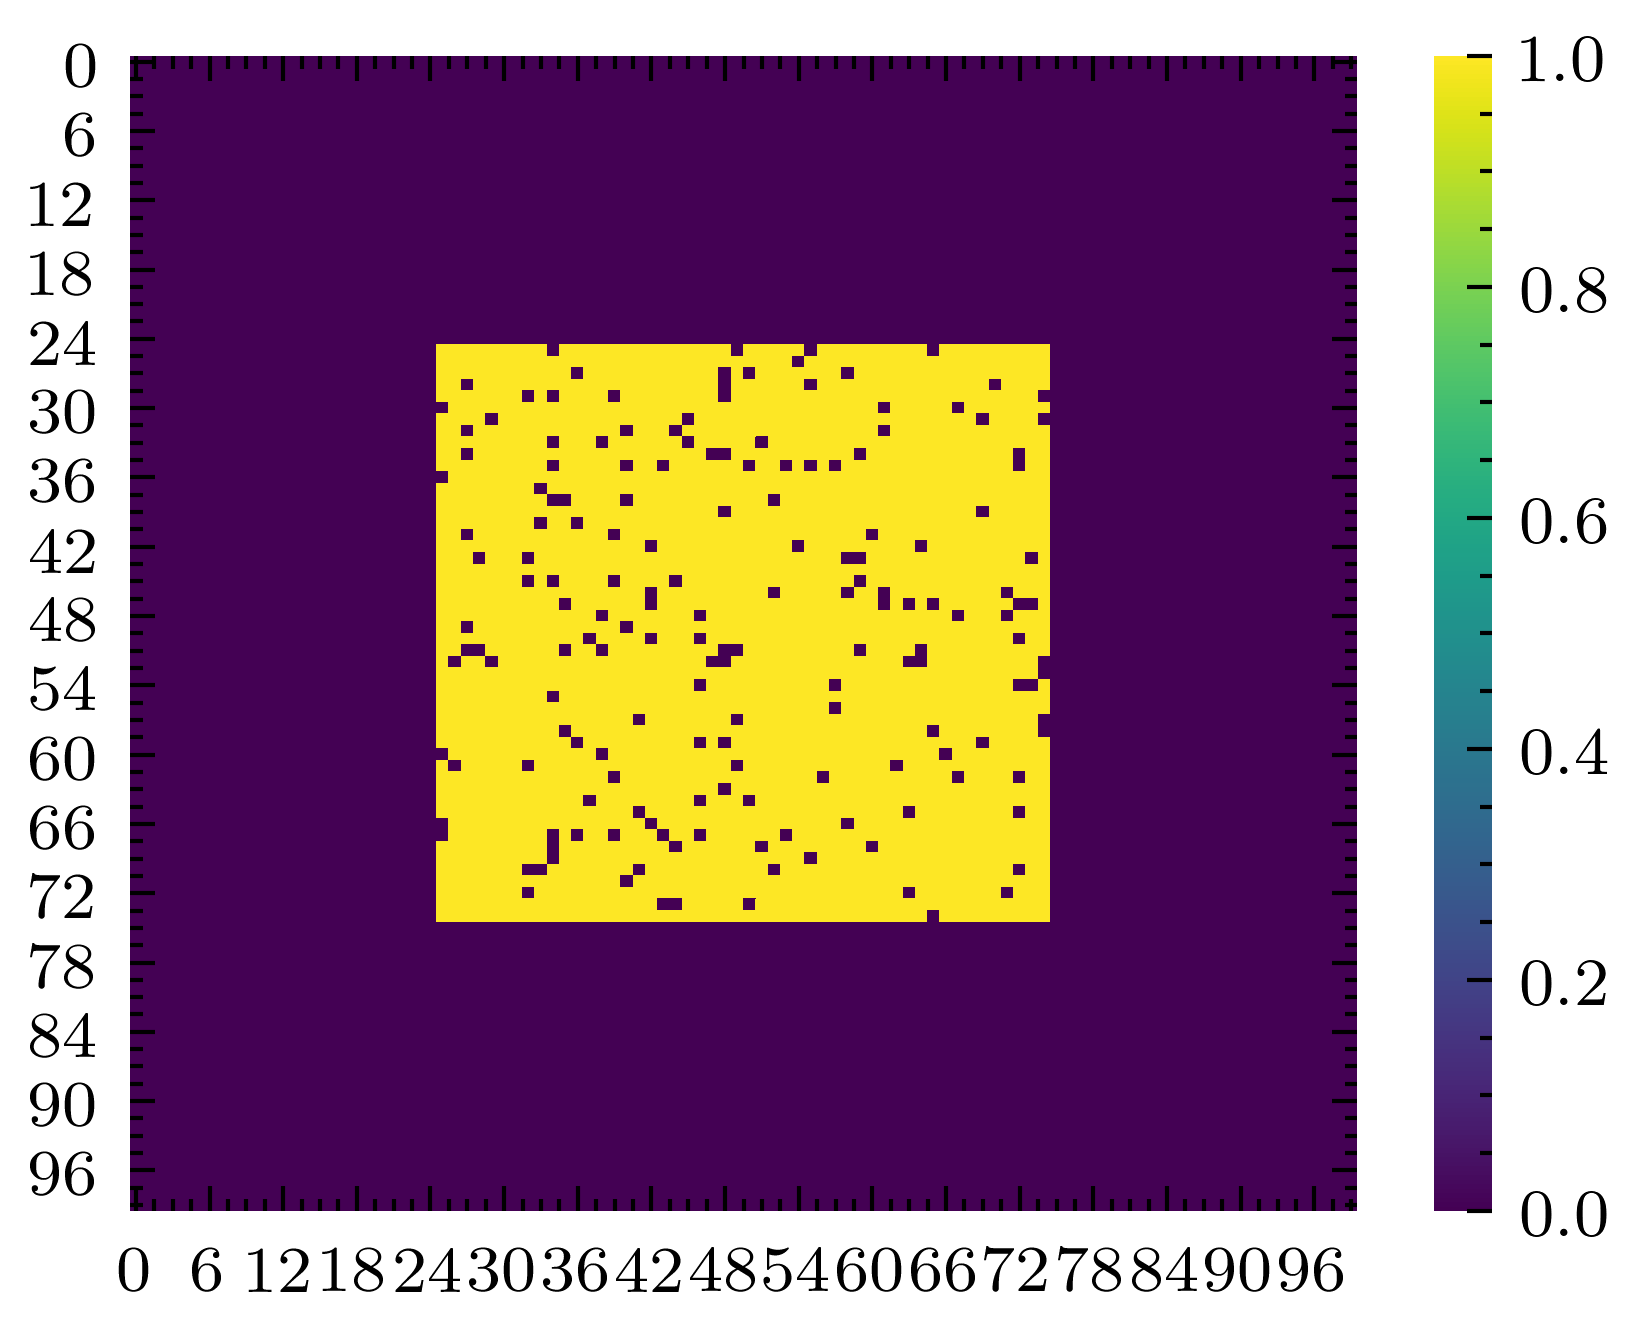
\includegraphics[width=\textwidth]{../img/data-aug/2d/center-coarse-dropout.png}
            \caption{Coarse Dropout}
            \end{subfigure}    

          \begin{subfigure}[b]{0.45\textwidth}
            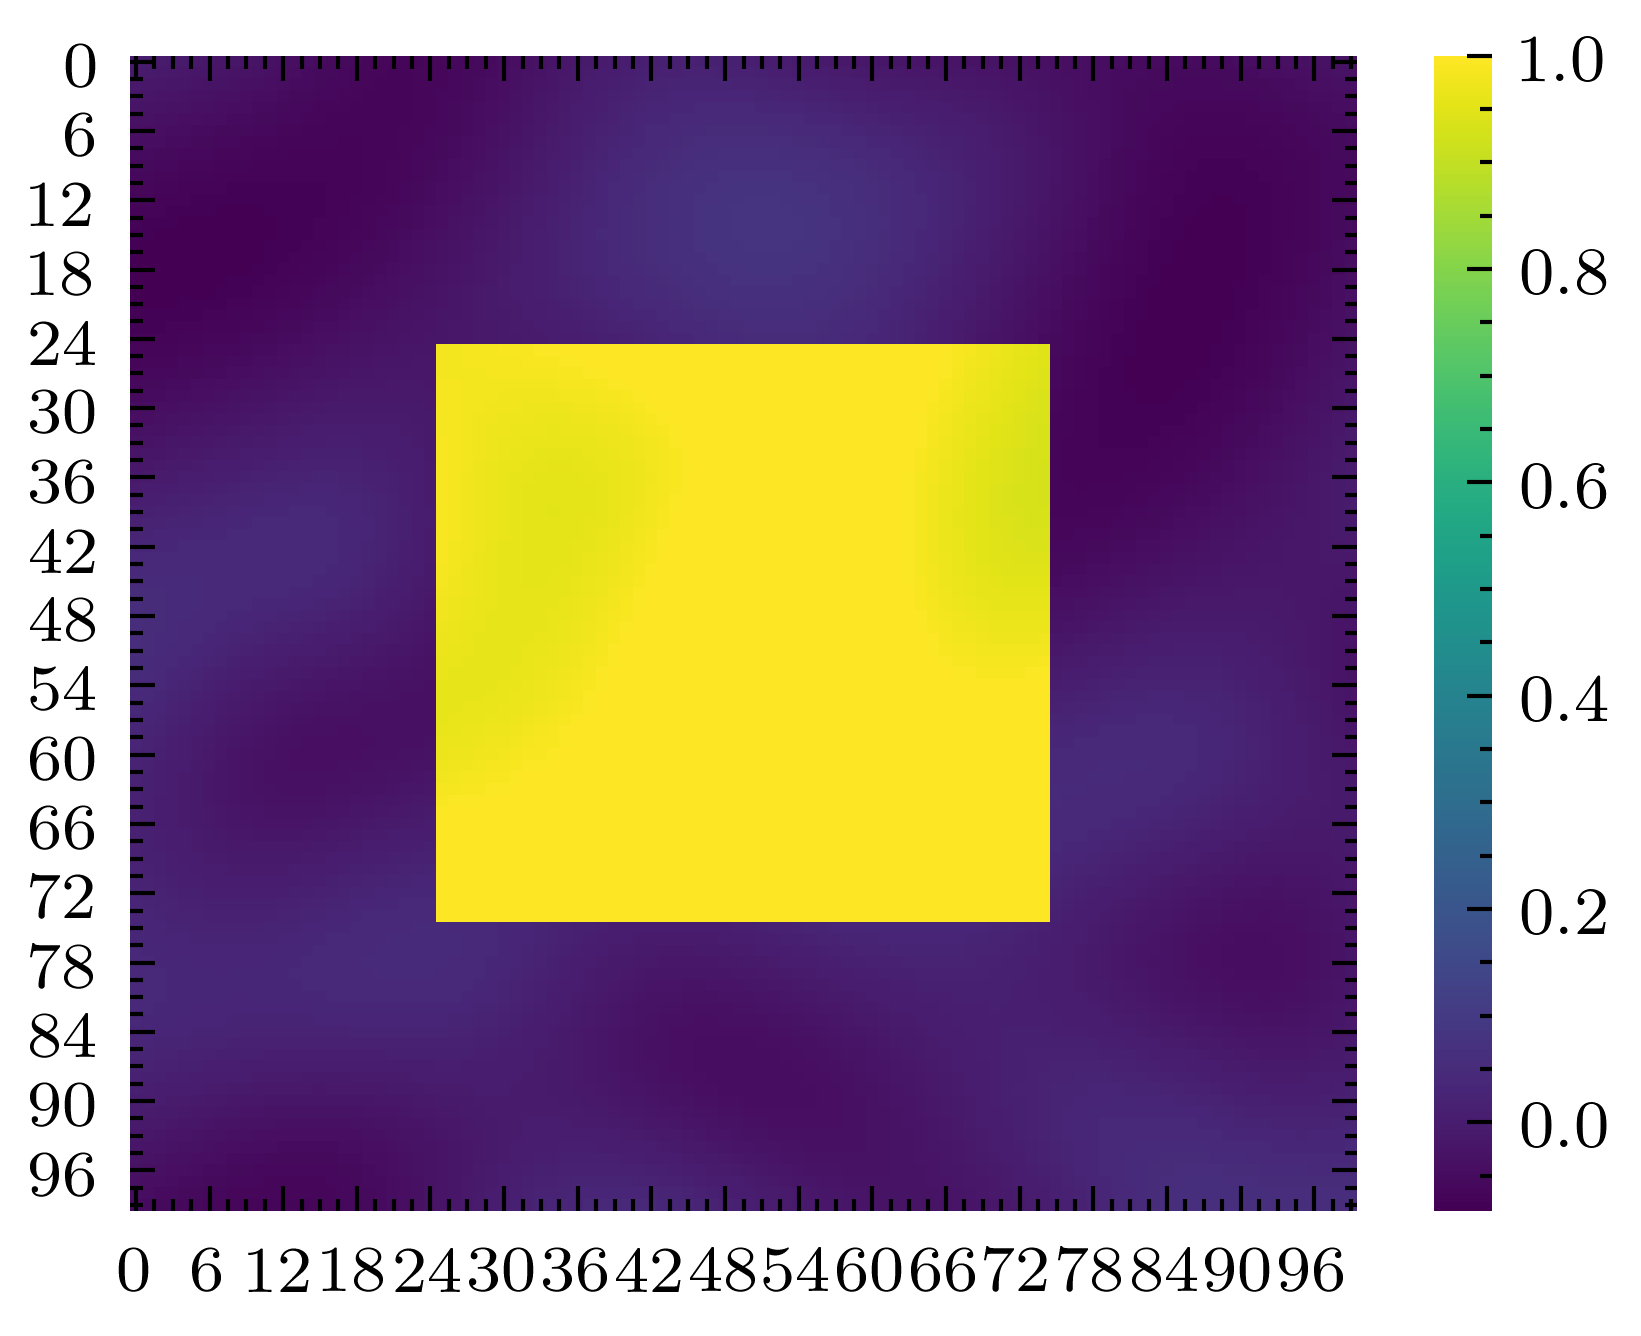
\includegraphics[width=\textwidth]{../img/data-aug/2d/center-simplex.png}
            \caption{Simplex Noise}

        \end{subfigure}    
        \begin{subfigure}[b]{0.45\textwidth}
            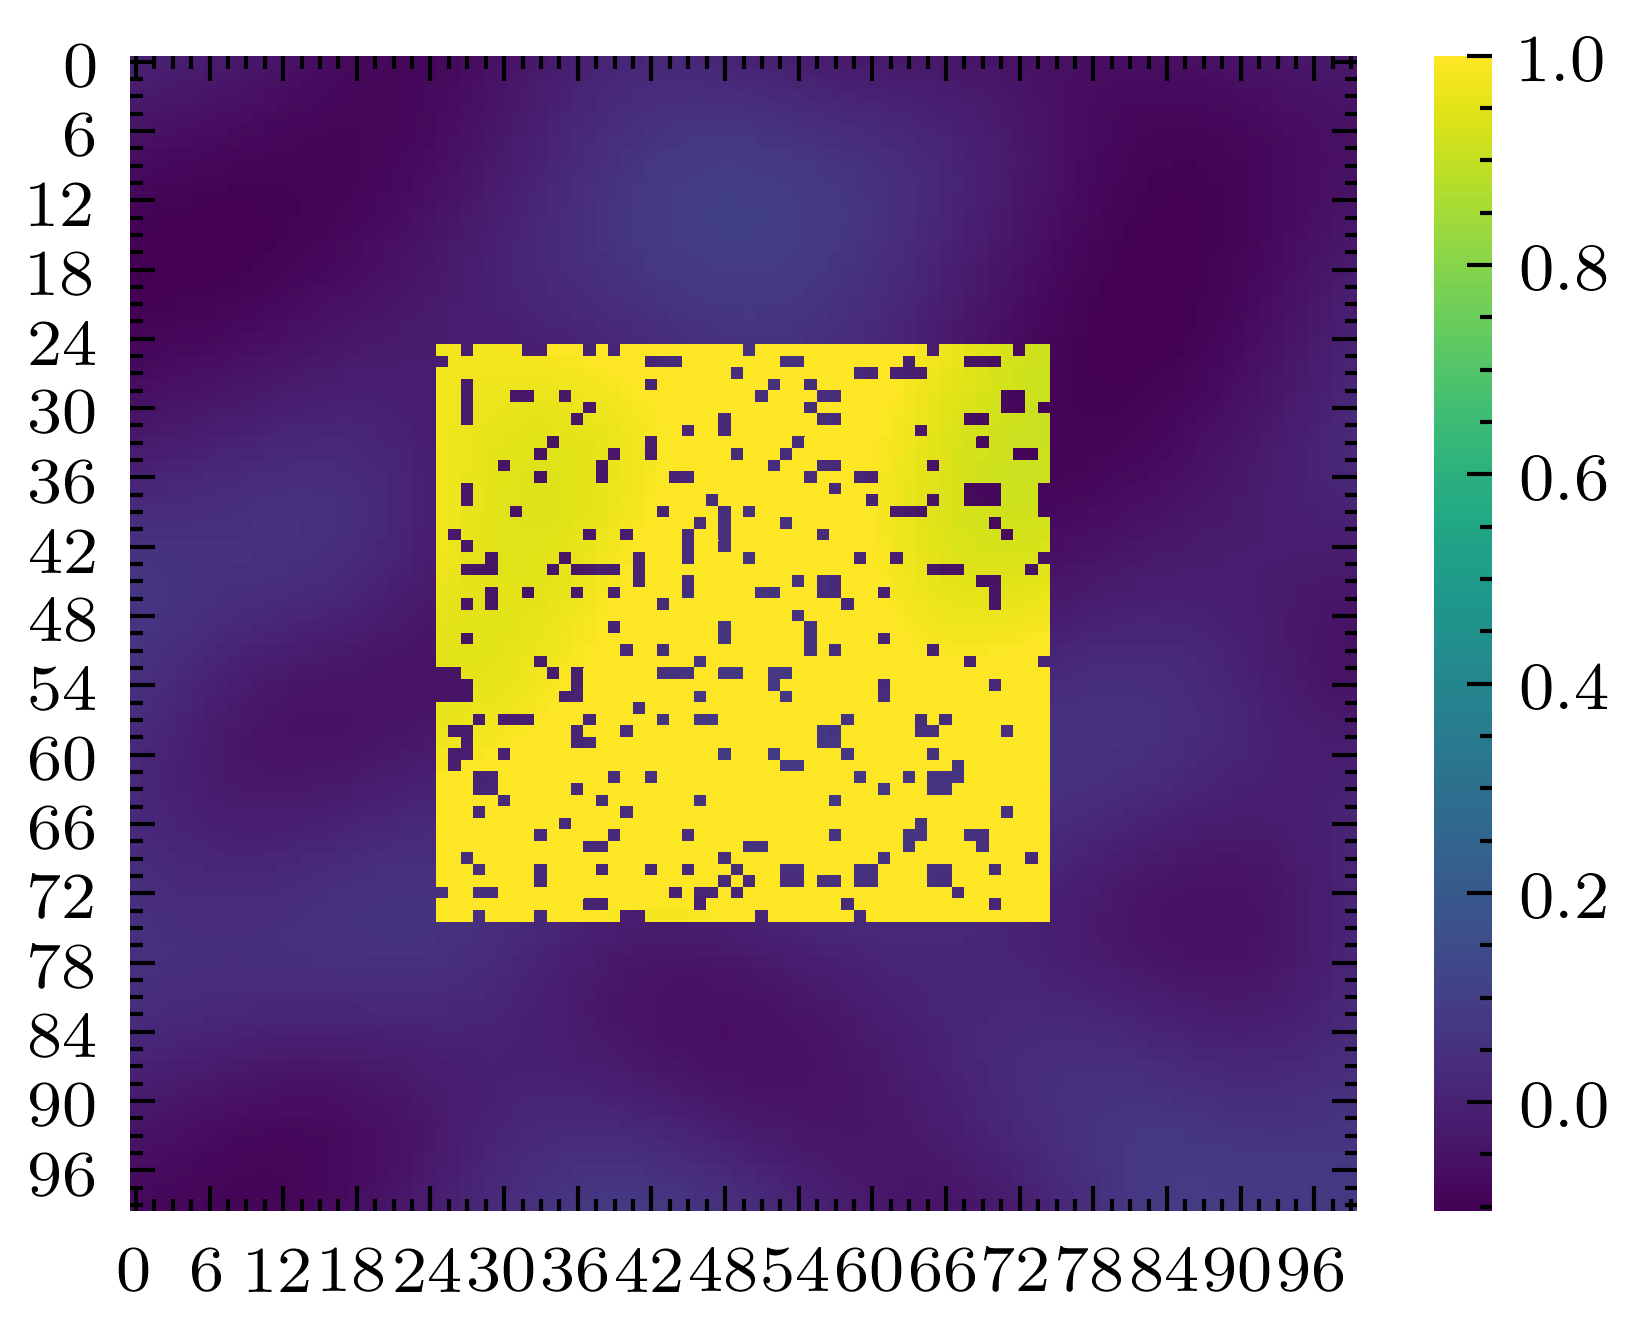
\includegraphics[width=\textwidth]{../img/data-aug/2d/center-aug.png}
            \caption{Final result}
        \end{subfigure}    
    \label{fig: square-patch-aug}
    \caption{Data augmentation}    
\end{figure}
It follows an other set of figures that shows the data augmentation we utilised on different inputs.

\begin{figure}[H]
    \centering
        \begin{subfigure}[b]{0.45\textwidth}
            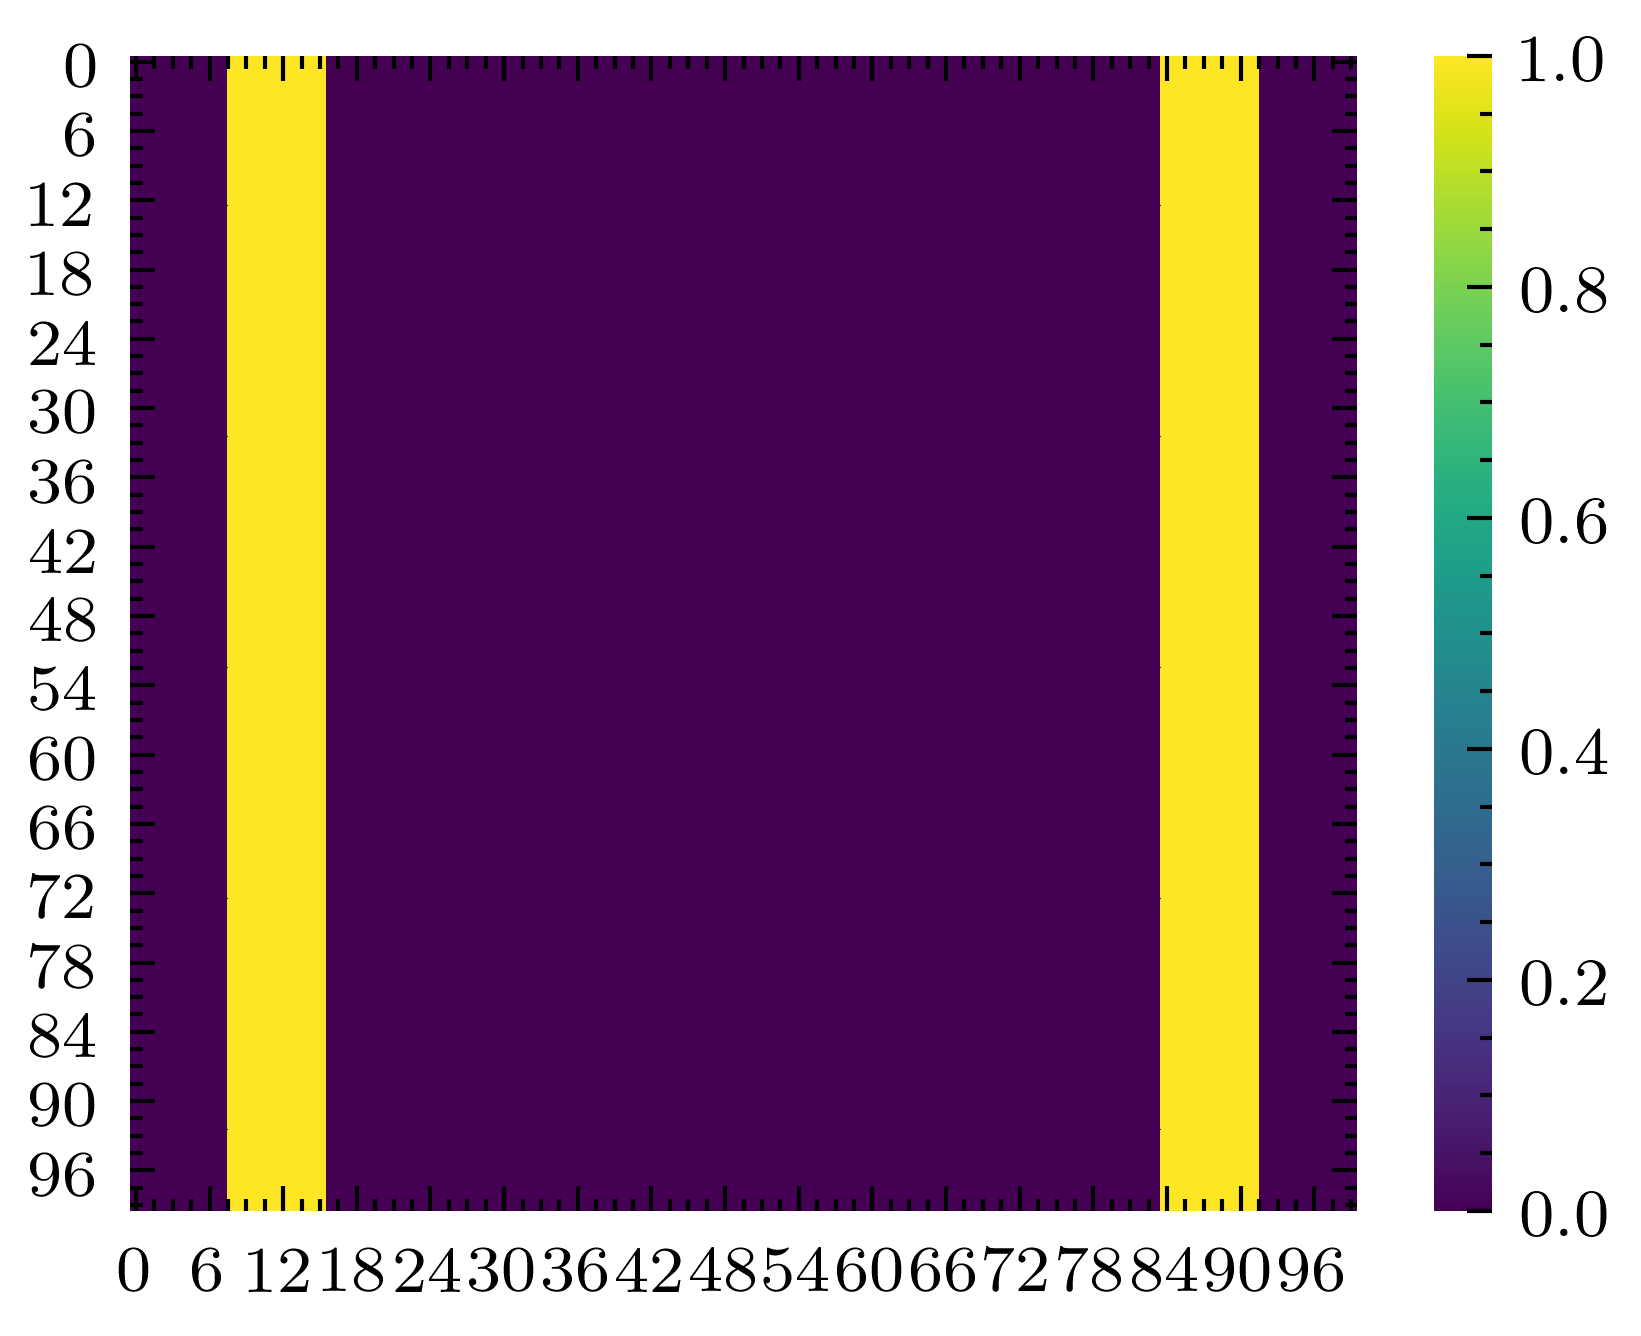
\includegraphics[width=\textwidth]{../img/data-aug/2d/wall.png}
            \caption{Walls}
        \end{subfigure}
        \begin{subfigure}[b]{0.45\linewidth}
            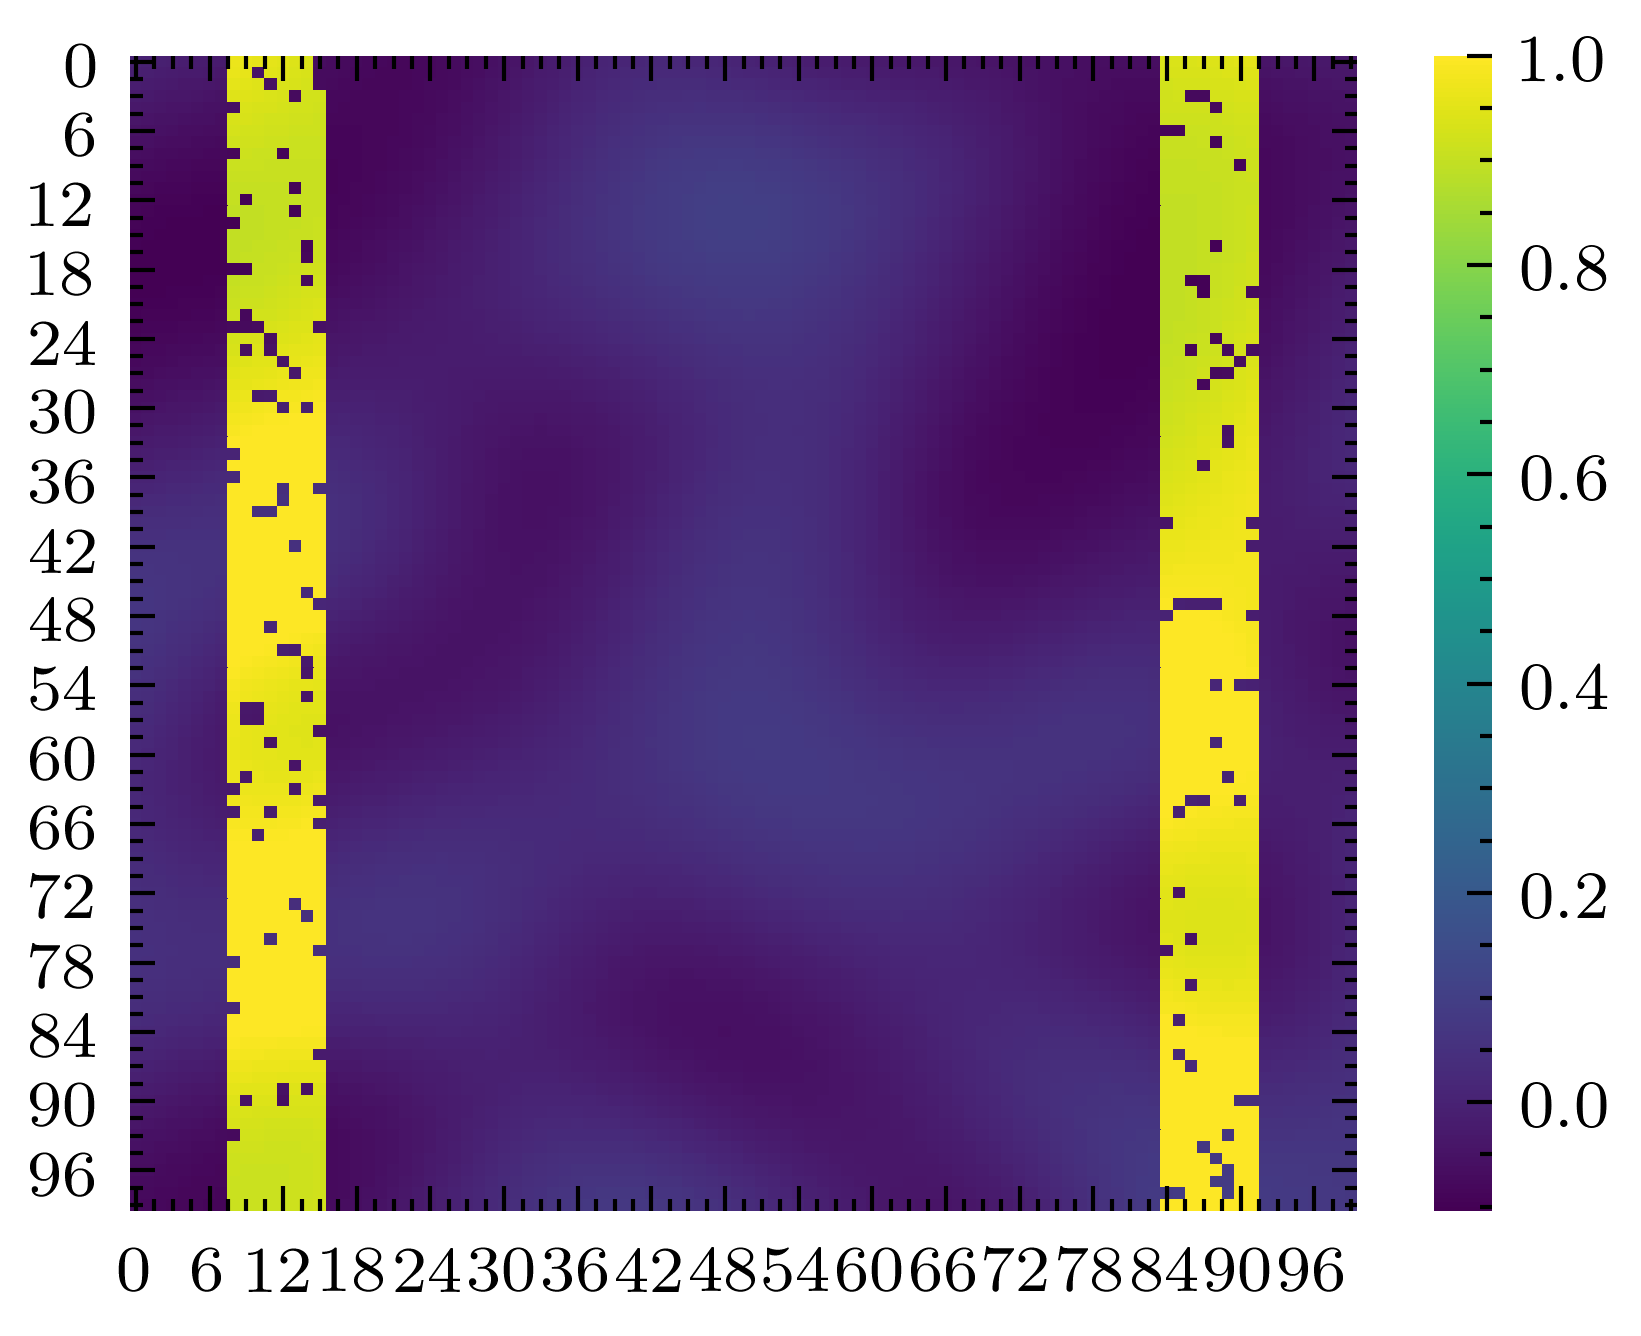
\includegraphics[width=\textwidth]{../img/data-aug/2d/wall-aug.png}
            \caption{Walls aug}
        \end{subfigure}    
        \begin{subfigure}[b]{0.45\textwidth}
            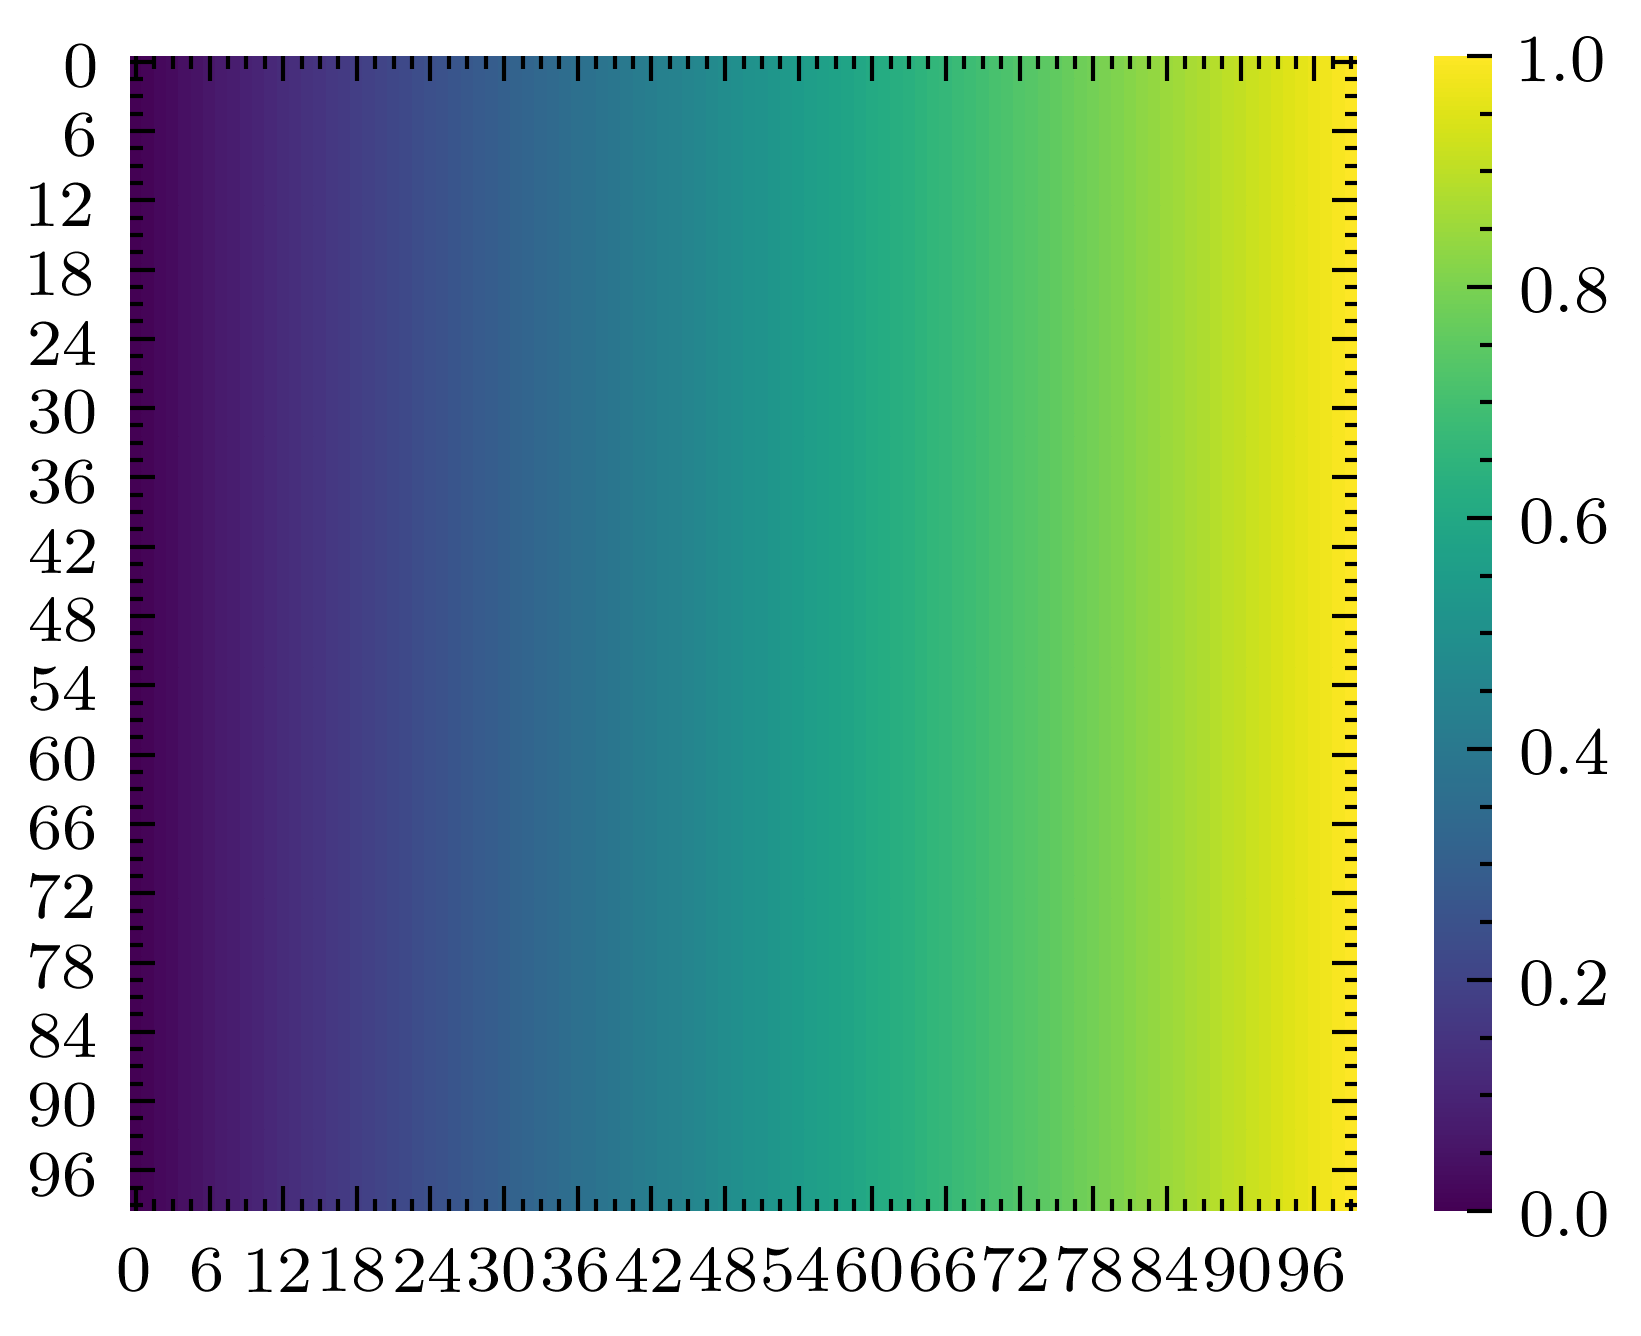
\includegraphics[width=\textwidth]{../img/data-aug/2d/ramp.png}
            \caption{Ramp}
        \end{subfigure}
        \begin{subfigure}[b]{0.45\linewidth}
            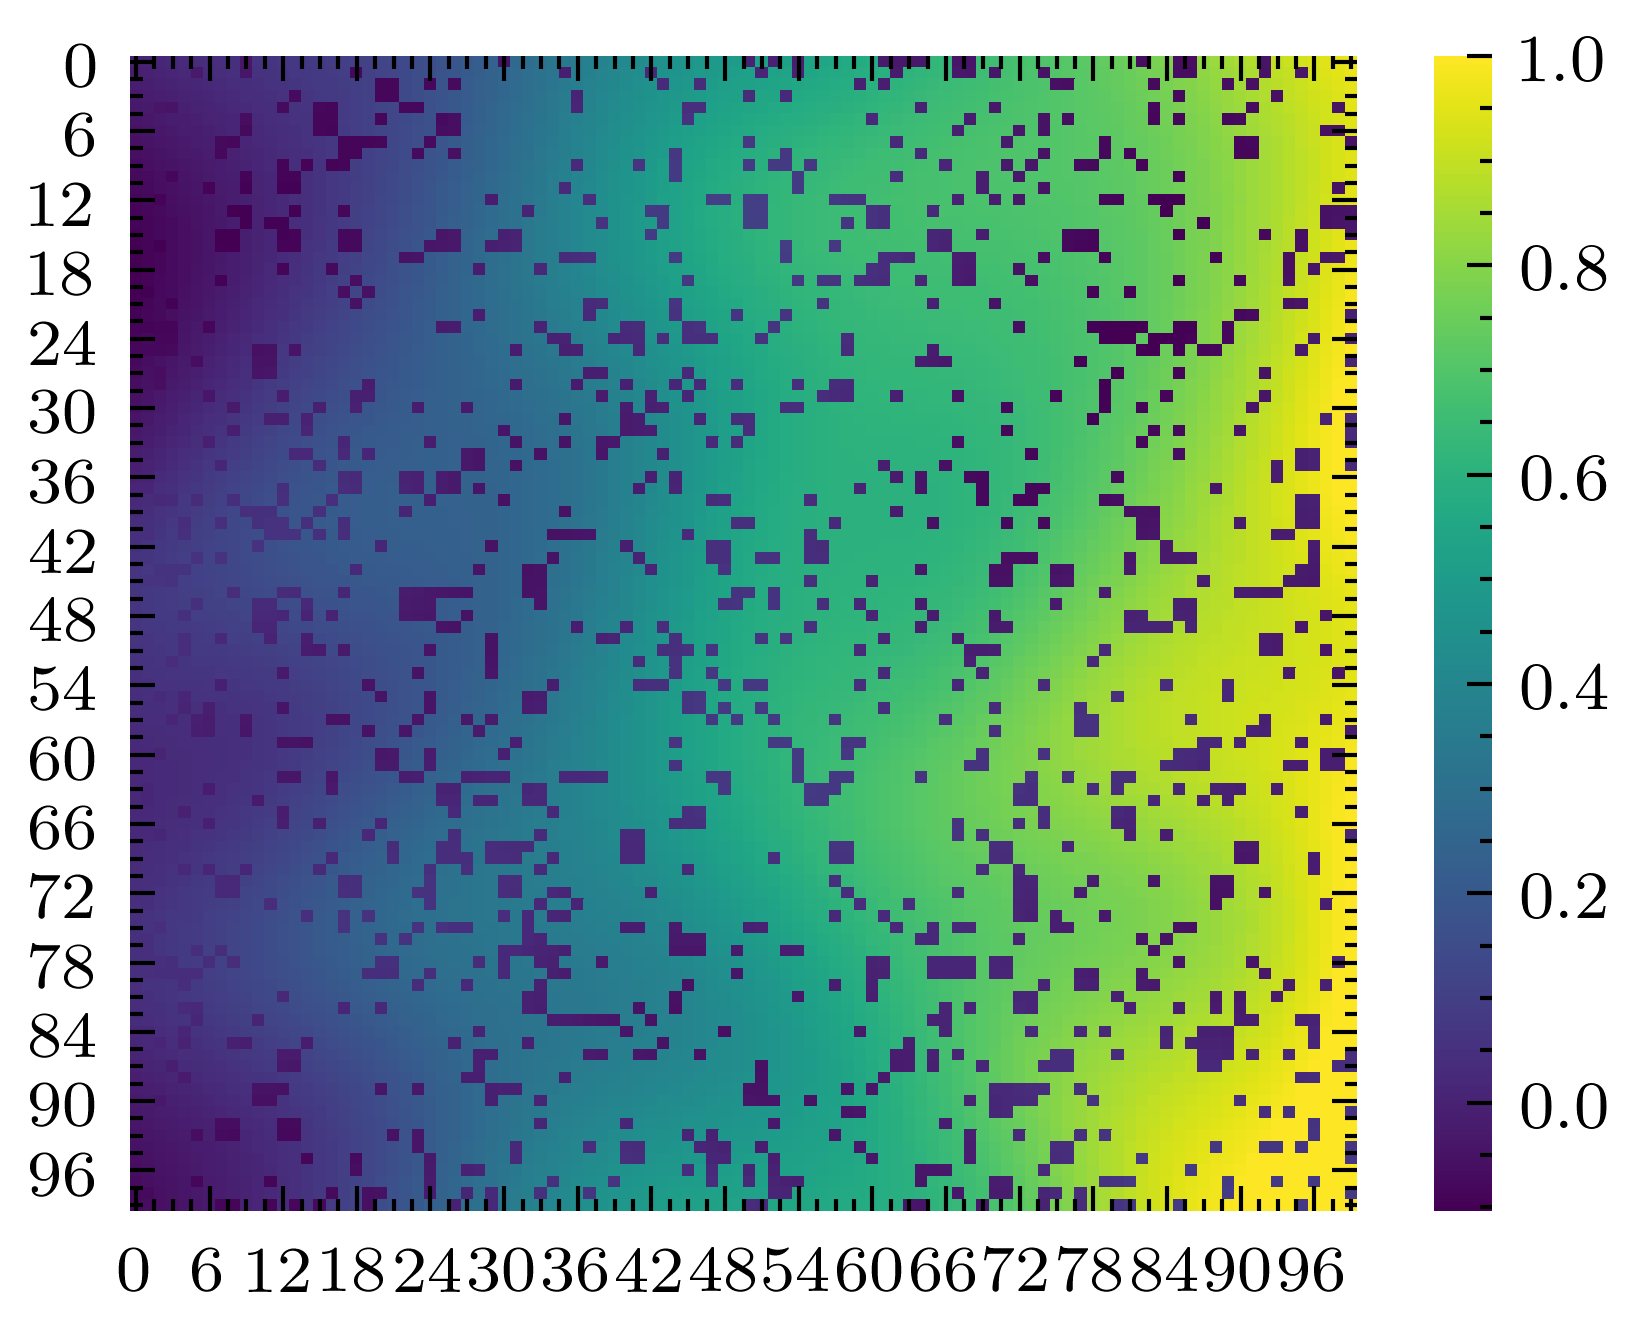
\includegraphics[width=\textwidth]{../img/data-aug/2d/ramp-aug.png}
            \caption{ramp aug}
        \end{subfigure}    
    \label{fig: others-aug}
    \caption{Wall}    
\end{figure}
\todo[inline]{add the parameters that we set}
In all the traning epochs, we apply data-augmentation to each input image $x$ with a probability of $0.8$. Dropout has a probability between $0.05$ and $0.1$. Coarse dropout with a probability of $0.02$ and $0.1$ with a size of the lower resolution image from which to sample the dropout between $0.6$ and $0.8$. Simplex noise with a feature size between $1$ and $50$ with a random scaling factor between $6$ and $10$. 
\end{document}
% \documentclass[../document.tex]{subfiles}
\begin{document}
\section{Results}
In the section we show and evaluate the model's results. We will start by presenting to the reader the networks score on each metric, then we will use the best model to predict the traversability in real world terrains. 
\subsection{Experiment Setup}
\subsubsection{Hardware}
We run all the experiment on a Ubuntu 18.10  work station equipped with a Ryzen 2700x, a powerful CPU with 8 cores and 16 threads, and a NVIDIA 1080 GPU with 8GB of dedicated RAM.
\subsubsection{Dataset}
To perform classification, we select a threshold of $0.2$m on a time window, $\Delta t$, of two seconds to label the patches, meaning that a patch with an advancement less than $20$ centimeters is labeled as \emph{no traversable} and viceversa. The  This processed is explained in detail in the previous chapter. While for the regression, we did not label the patch and directly regress on the advancement.

Initially, to train the models we first use Standard Gradient Descent with momentum set to $0.95$ and weight decay to $1e-4$ with an initial learning rate of $1e-3$ as was originally proposed to train residual network \cite{he2015deep}. However, we later utilize Leslie Smith's 1cycle policy \cite{1cycle} that allows us to trian the network faster and with an higher accuracy. We minimise the binary Cross Entropy for the classifier and the  Mean Square Error (MSE) for the regressor.
\subsubsection{Experimental validation}
We select as \emph{validation} set ten percent of the training data. Since we store each run of Krock as a \emph{.csv} file, validation and train set do not overlap. 
The test set is composed entirely by the Quarry map, a real world scenario. Table \ref{table: maps} tells in detail the configuration used in each map of all sets.

We also evaluate the model on the following additonal maps
\todo[inline]{ add arck rocks}
\subsubsection{Metrics}

\paragraph{Classification:} To evaluate the model's classification performance we used two metrics: \emph{accuracy} and \emph{AUC-ROC Curve}. Accuracy scores the number of correct predictions made by the network while AUC-ROC Curve represents degree or measure of separability, informally it tells how much model is capable of distinguishing between classes. For each experiment, we select the model with the higher AUC-ROC Curve during training to be evaluated on the test set.



\paragraph{Regression:} We used the Mean Square Error to evaluate the model's performance.
\subsection{Quantitative Results}
\subsubsection{Model selection}
We compared two different \emph{micro-resnet} and the \emph{vanilla} cnn from the previous Chapter. We evaluate those models using a time window of two second, a threshold of $20$cm and the data augmentation techniques described before. We run five experiments per architecture and we select the best performing network, the results are showed in the following table. 

\begin{table*}[h]
  \centering
  \ra{1.2}
  \begin{tabular}{@{}lcccc@{}}
  \toprule
   && Vanilla & \multicolumn{2}{c}{MicroResnetSE} \\
  \cline{3-5}
  && & $3\times 3$ stride $1$ & $7\times7$ stride $2$\\ 
  \cline{3-5}
  \multirow{2}{*}{AUC} & Top & 0.892 & 0.888 & \textbf{0.896}\\
   & Mean & \textbf{0.890} & 0.883 & 0.888\\
  \cline{1-5}
  Params & & 974,351 & 313,642 & 314,282  \\
  \bottomrule   
\end{tabular}
\caption{Model comparison on the test set.}
\end{table*}
\todo[inline]{Luca told me is better to split the models like Model1 and Model2 etc}

Based on this data We select \emph{micro-resnet} with squeeze and excitation and a starting convolution's kernel size of $7\times7$ with stride of $2$. This model has one third of the parameter of the origal model proposed by Chavez-Garcia et all \cite{omar2018traversability}. 

As proof of work, we also train the best network architecture, MicroResnetSE with a first convolution's kernel size of $7 \times 7$ and stride$=2$, with and without the Squeeze and Excitation operator.
\begin{table*}[h]
  \centering
  \ra{1.2}
  \begin{tabular}{@{}lccc@{}}
  \toprule
  &  MicroResnet$7\times7$ & MicroResnet$7\times7$-SE  & Improvement \\
  \cline{1-4}
   Top & 0.875 & \textbf{0.896} & $+0.021$ \\
   Mean & 0.867 & \textbf{0.888} & $+0.021$ \\
  \bottomrule   
\end{tabular}
\caption{AUC top value and mean value for MicroResnet with a fist convolution of $7\times7$ and stride $=2$ with and without the SE module. The improvement is the same.}
\end{table*}

\subsection{Final results}
The following table shows in deep the score of the best network for each dataset.
\begin{table*}[h]
    \centering
    \ra{1.2}
    \begin{tabular}{@{}llccccc@{}}
    \toprule
    % \multicolumn{8}{c}{Quantitative evaluation in simulation} \\
    \multicolumn{2}{c}{Dataset} && \multicolumn{2}{c}{micro-resnet} & Size & Resolution(cm/px) \\
    \cmidrule{1-2} \cmidrule{4-5}
    Type     &  Name  & Samples & ACC  &  AUC    & & \\
    \toprule
      \multirow{3}{*}{Synthetic}  & Training   & 429312 & - & - & & 2\\
      &  Validation   & 44032 &  95.2 \% &  0.961 & & 2 \\
      & Arc Rocks & 37273 &  85.5 \% &  0.888 & & 2 \\
      \cmidrule{2-7}
    \multirow{3}{*}{\makecell[l]{Real\\evaluation}} & Quarry & 36224 &  88.2 \%&  0.896& & 2\\
    & foo & TODO & & & & \\
    & baaa & TODO & & & & \\
    \bottomrule   
\end{tabular}
\caption{Final results on different datasets.}
\end{table*}
\todo[inline]{I have actually never talk about surf rocks}
Moreover, we would like to also show the different steps we made to reach this result. The following table shows the metric's score without any data-augmentation.
\todo[inline]{add result with and without data agu}
Adding dropout increases the results.
\todo[inline]{table with results}
With dropout plus coarse dropout.
\todo[inline]{table with results}
\subsection{Qualitative results}
We qualitative evaluate the model predictions by showing the traversability probability on different maps in 3D as a texture. Specifically, we used a sliding window to extract the patches from the heightmaps and create a texture based on the model's output for the traversable class. We then apply this texture on the image and colour using a colormap. For each map we show the traversability from bottom to top, top to bottom, left to right and right to left since those are the most human understandable.
\subsubsection{Quarry}
% \todo[inline]{add quarry textures from bottom to top}

The first map we evaluate is Quarry. This maps has some interesting features, such as the three bis slopes and the rocky ground on top. We expect the trail on the slopes to be traversable at almost any rotation, expecially from left to right and viceversa. While, the top part should be not traversable in any case. The following figure shows the traversability probability on the map.
\begin{figure}[H]
\centering
\begin{subfigure}[b]{0.45\textwidth}
  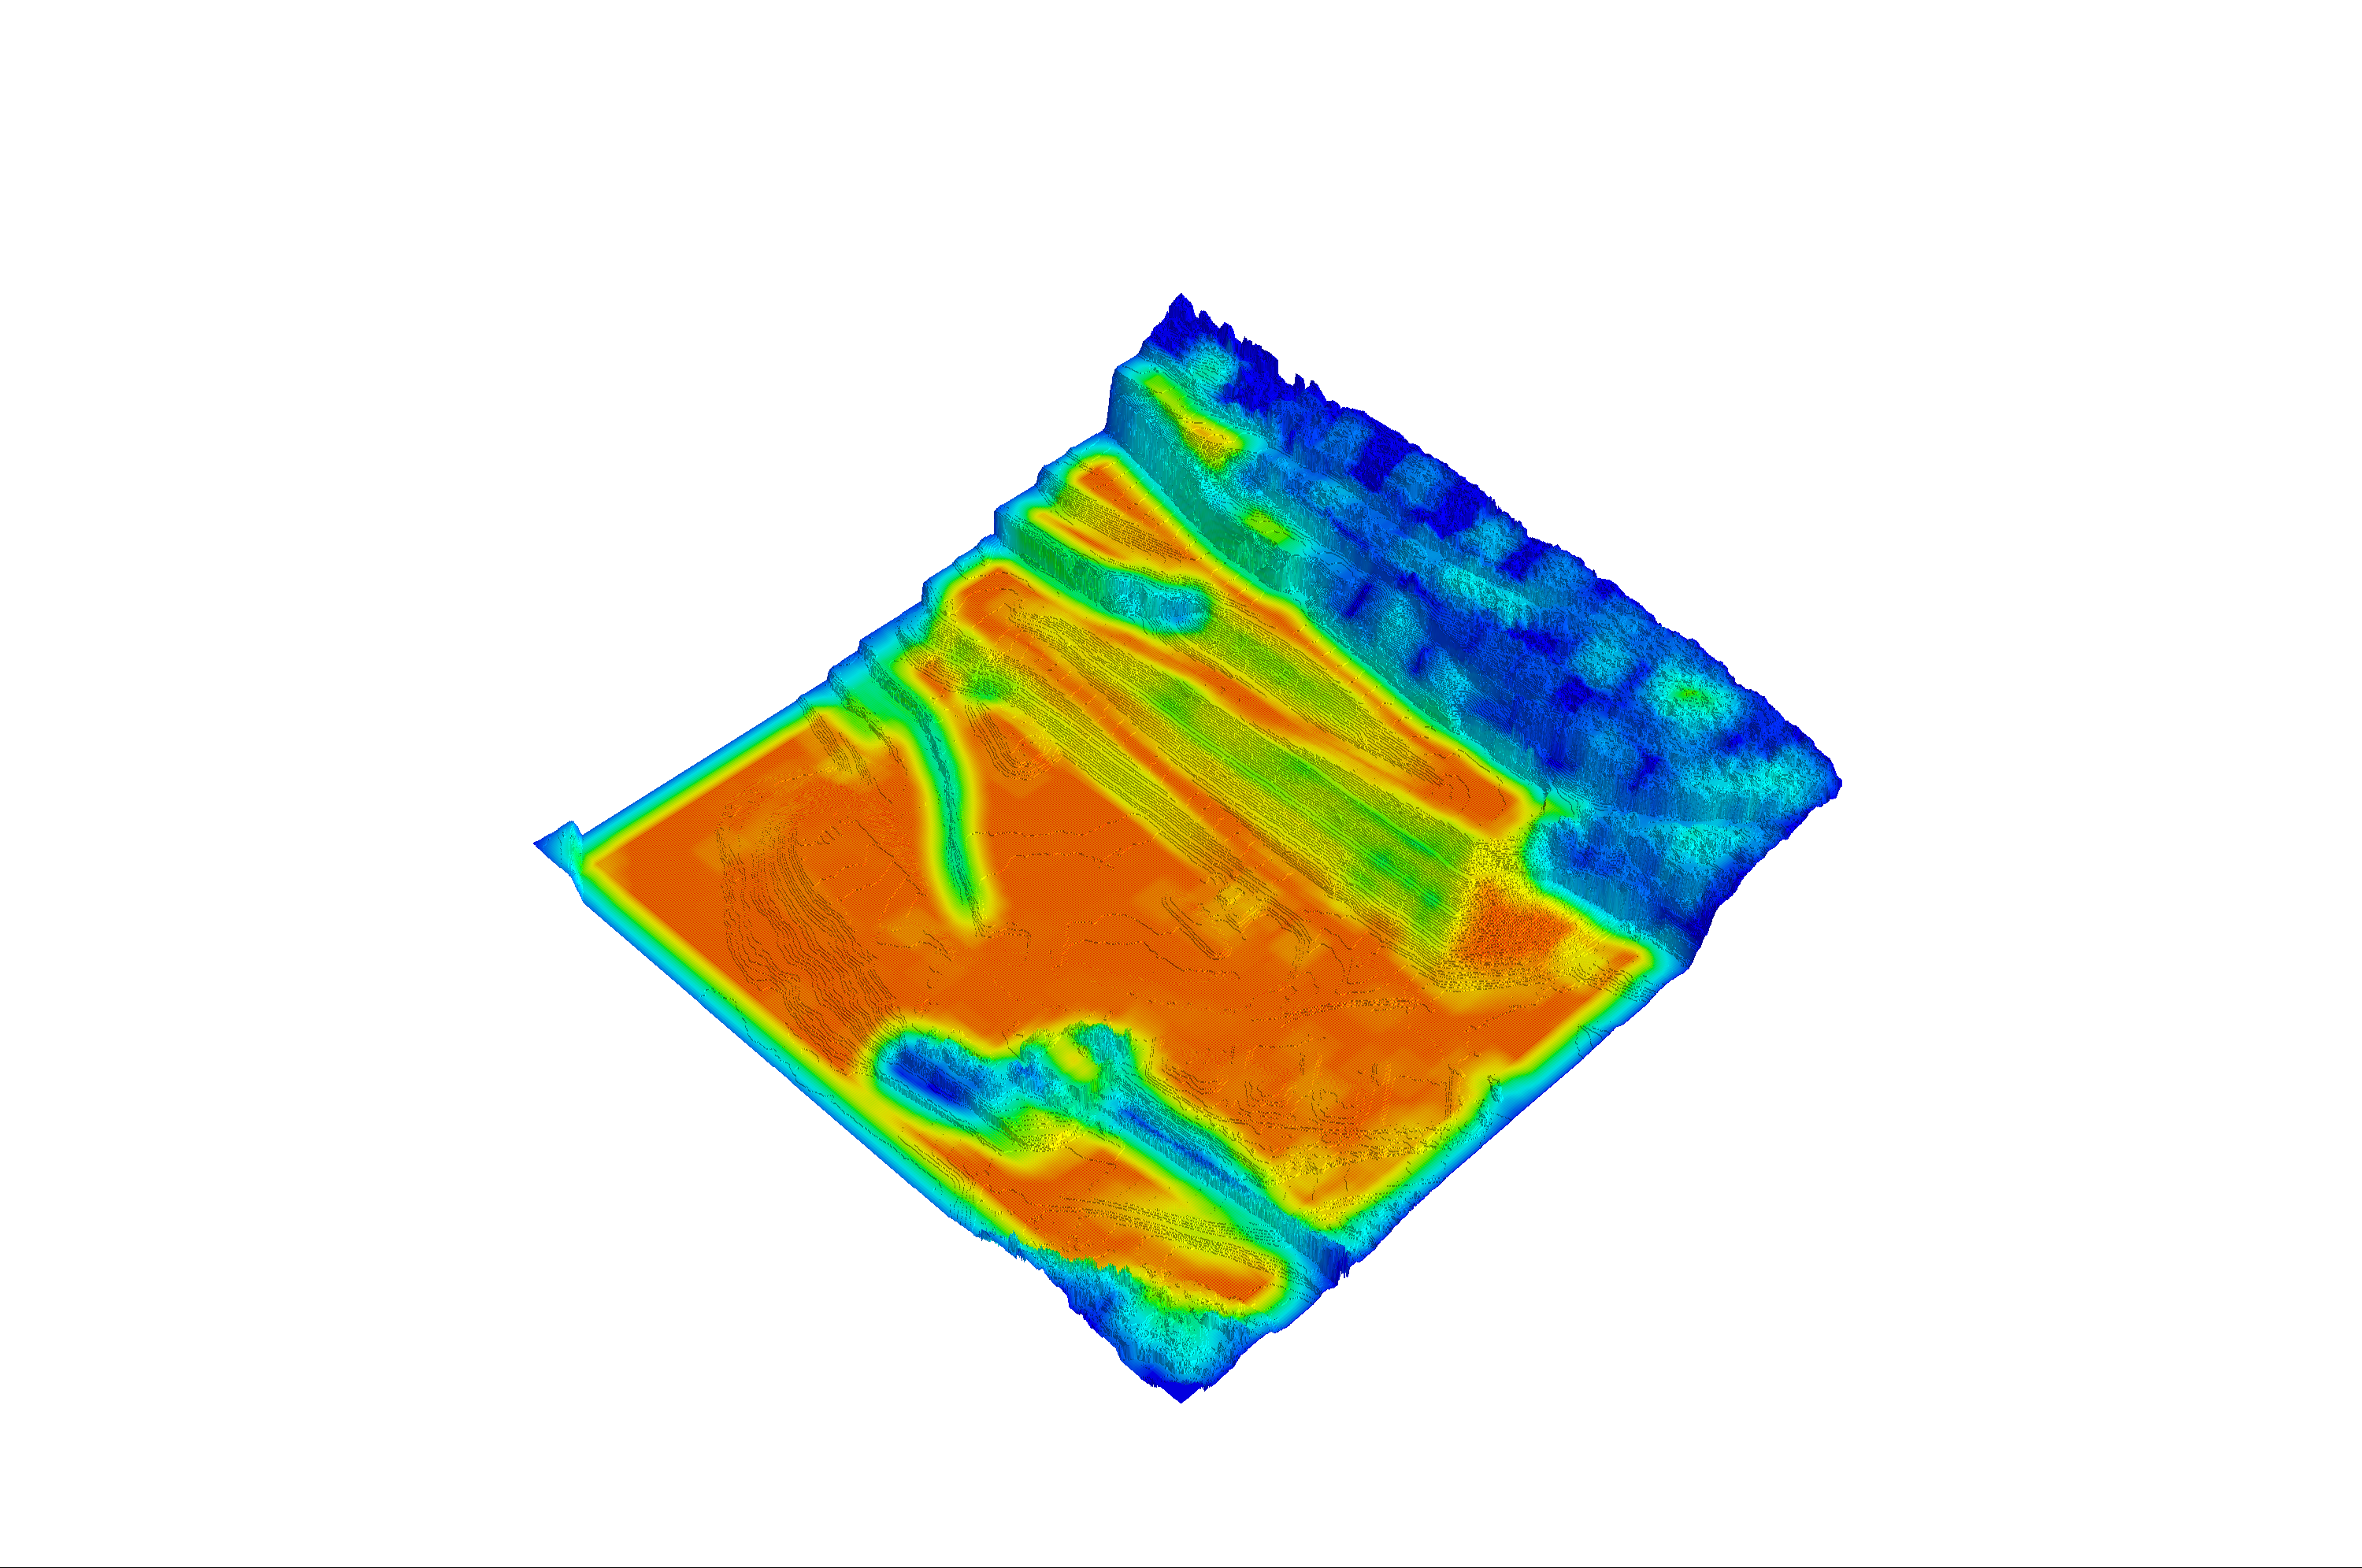
\includegraphics[width=\linewidth]{../img/4/traversability/quarry/270.png}  
\end{subfigure}
\begin{subfigure}[b]{0.45\textwidth}
    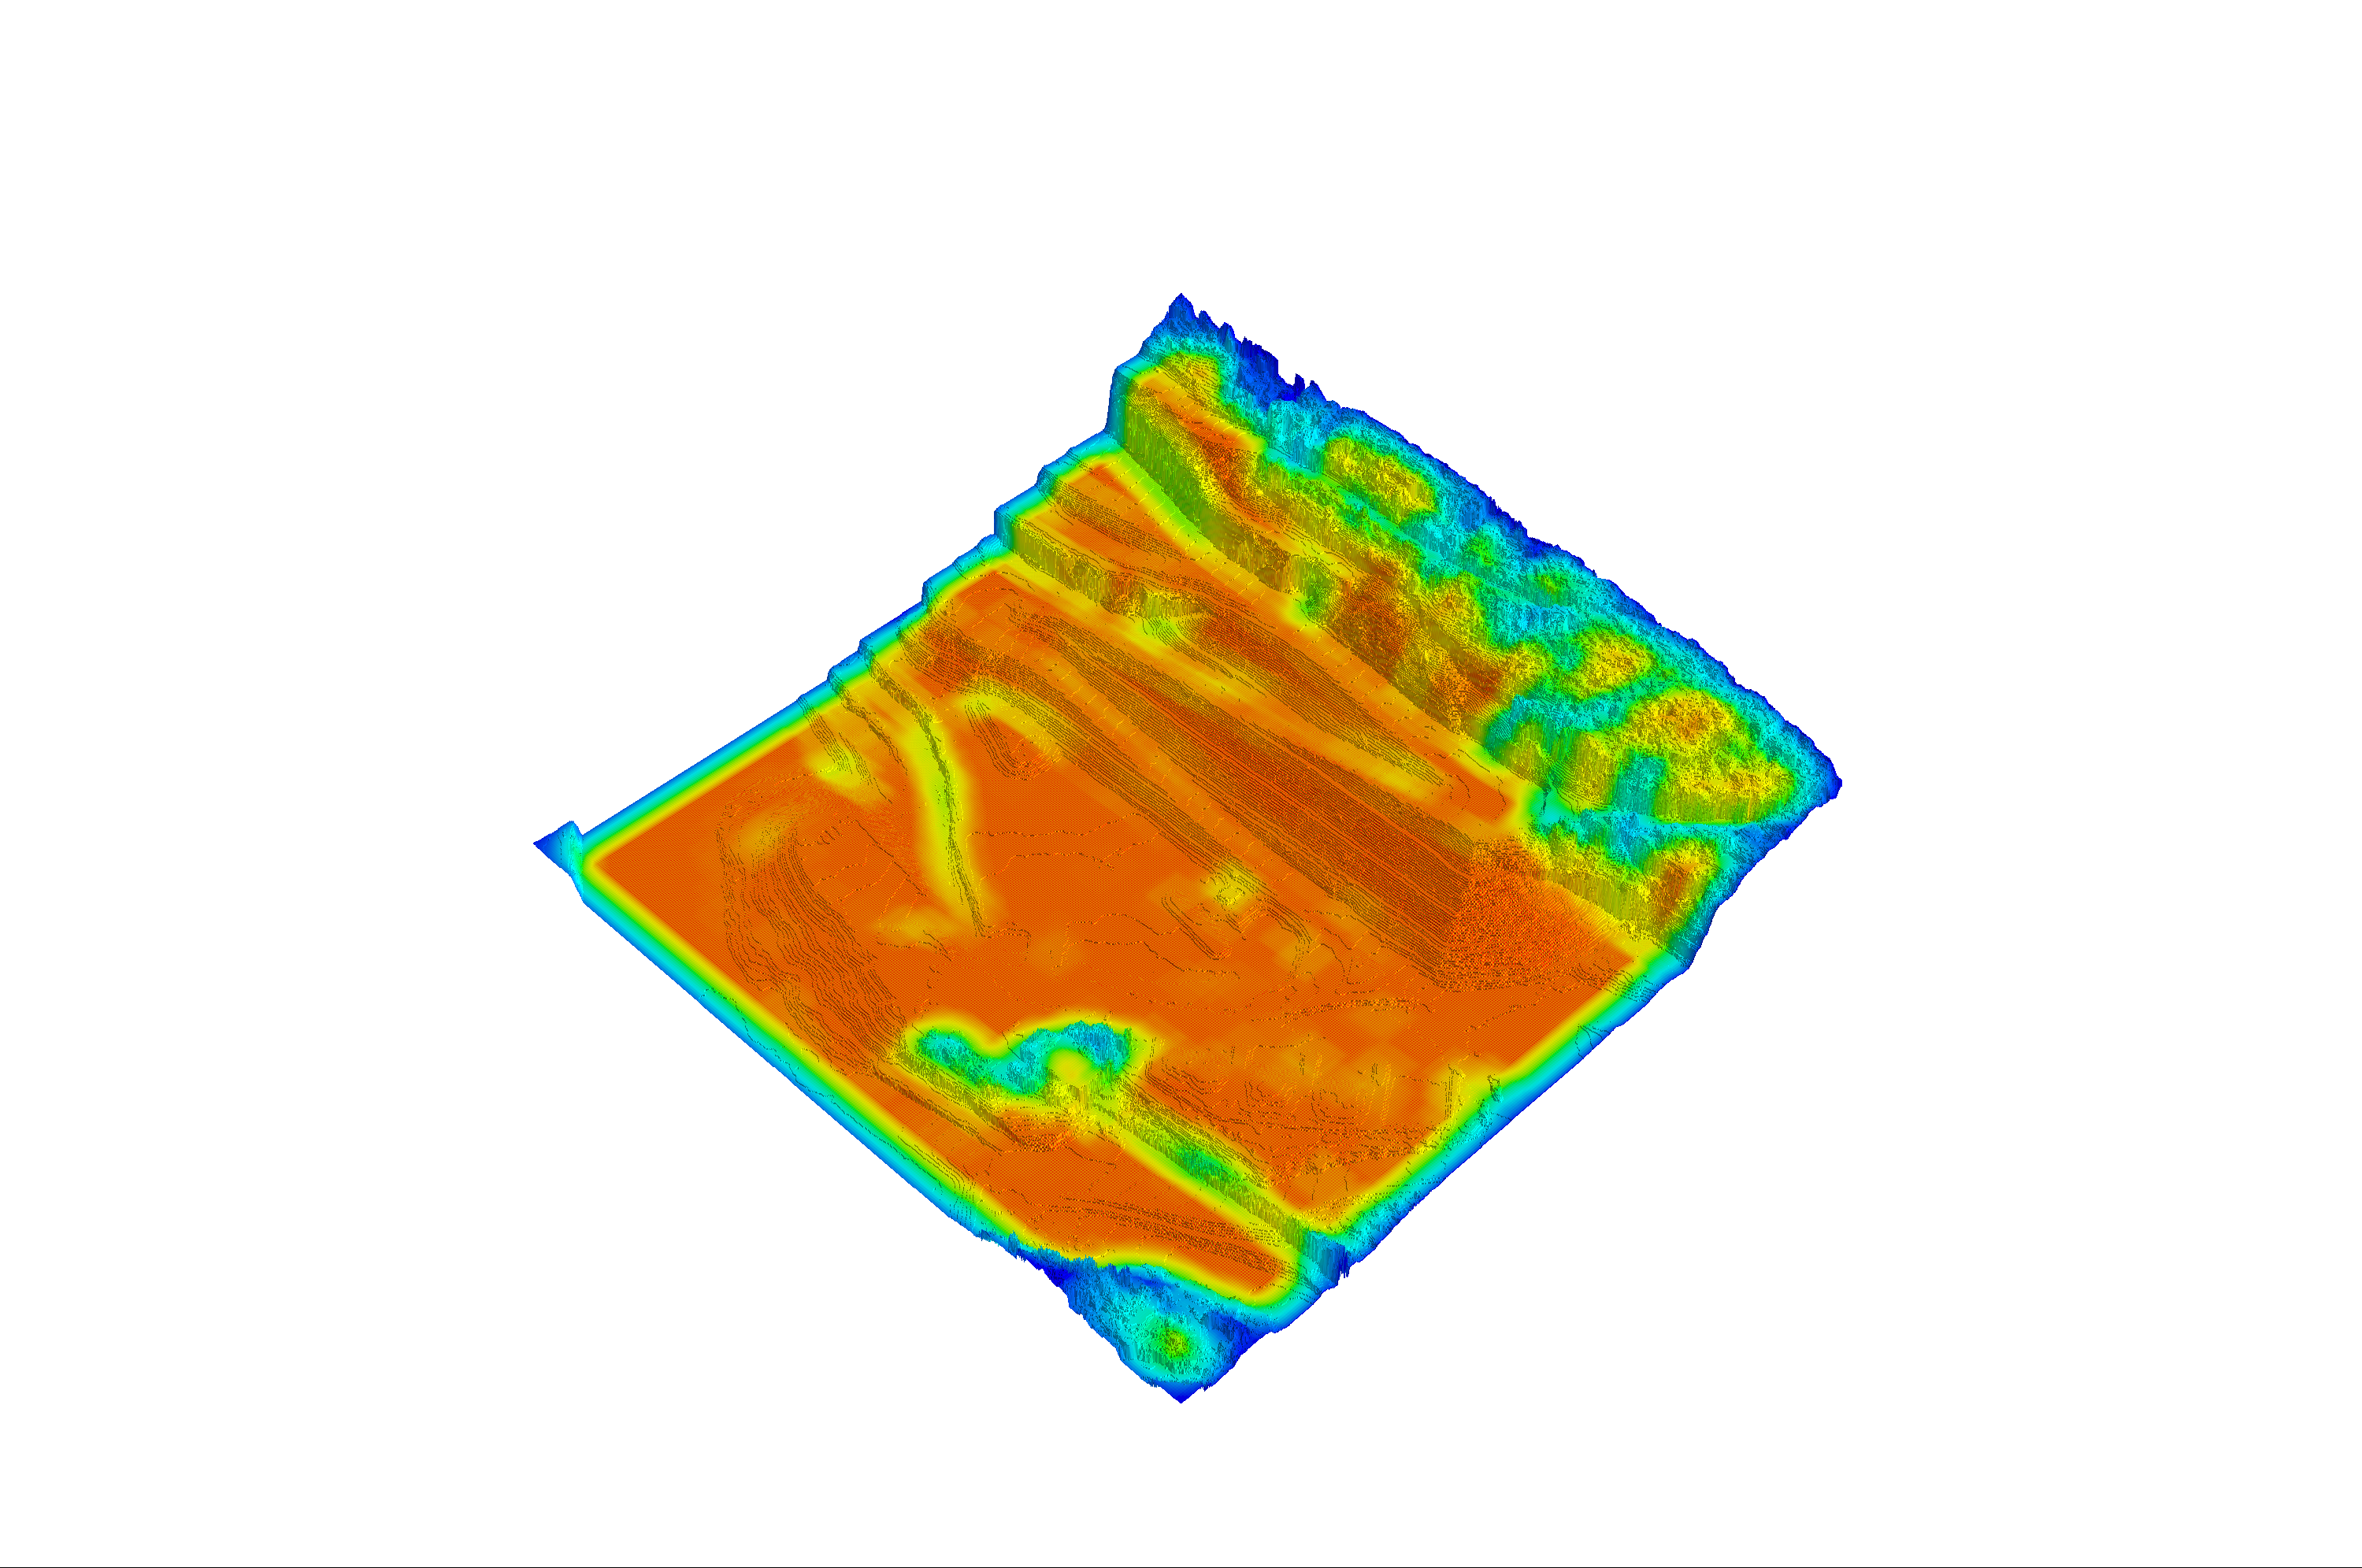
\includegraphics[width=\linewidth]{../img/4/traversability/quarry/0.png}  
\end{subfigure}
\begin{subfigure}[b]{0.45\textwidth}
  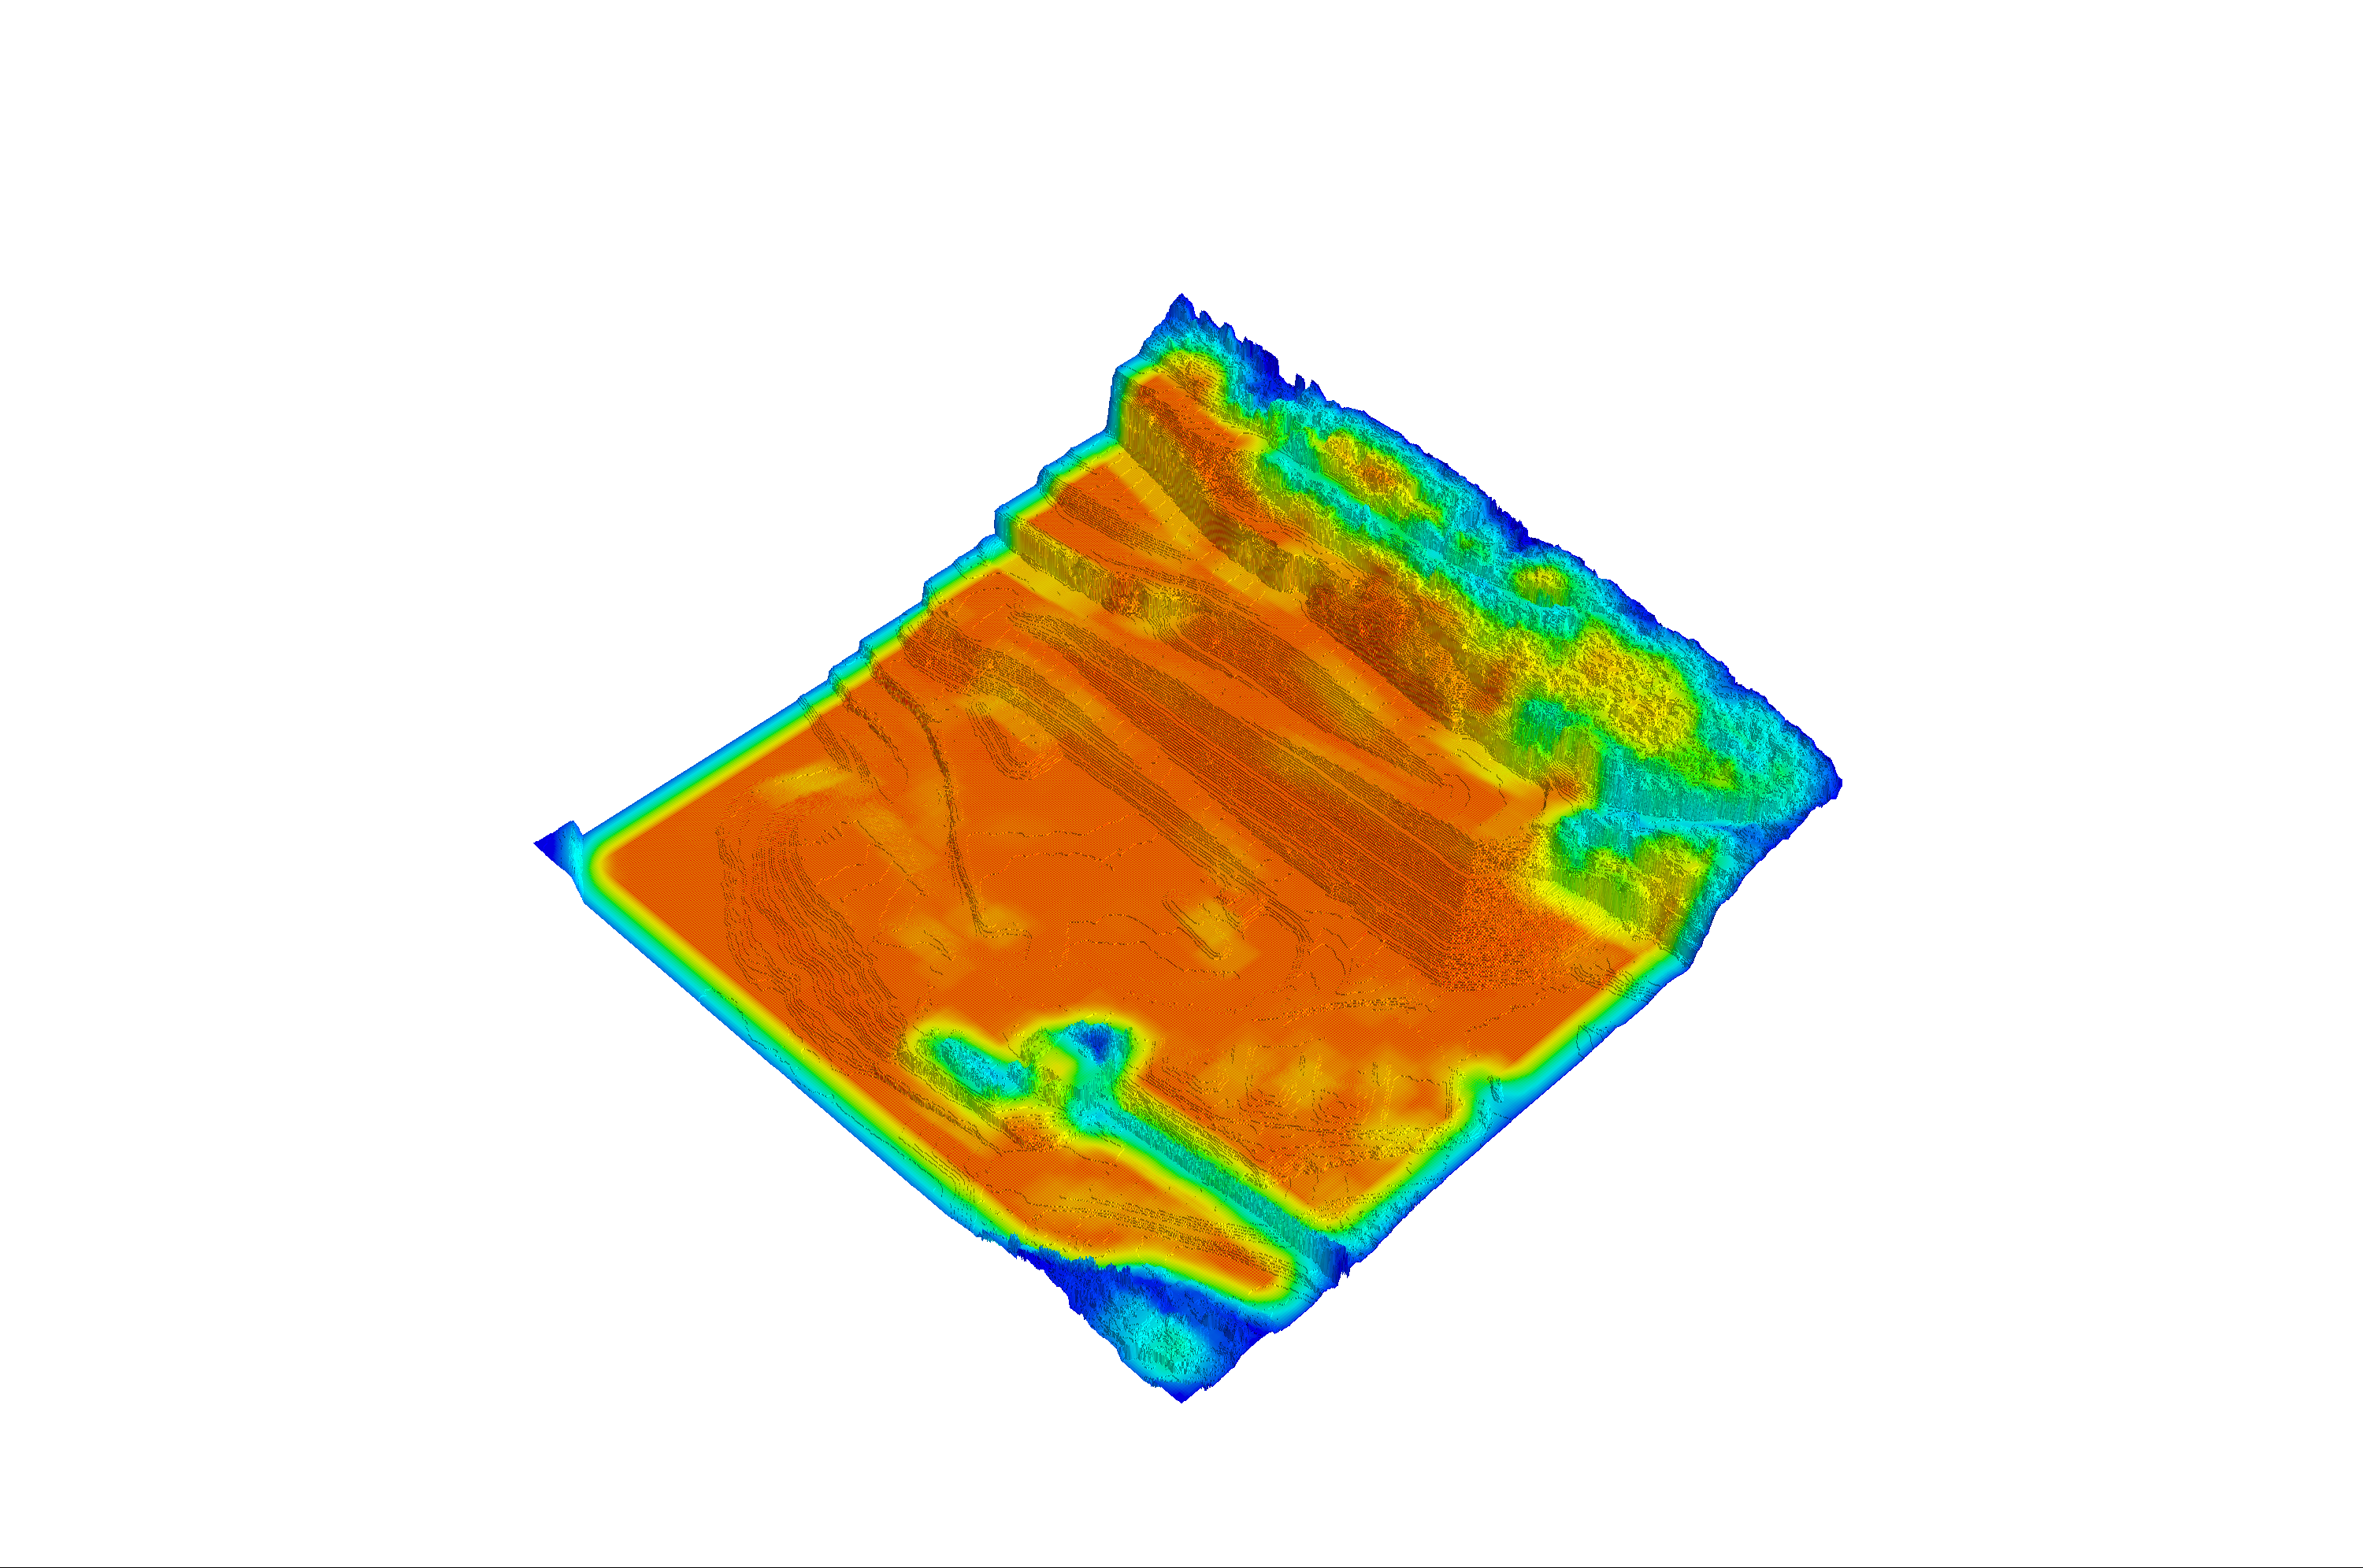
\includegraphics[width=\linewidth]{../img/4/traversability/quarry/90.png}  
\end{subfigure}
\begin{subfigure}[b]{0.45\textwidth}
    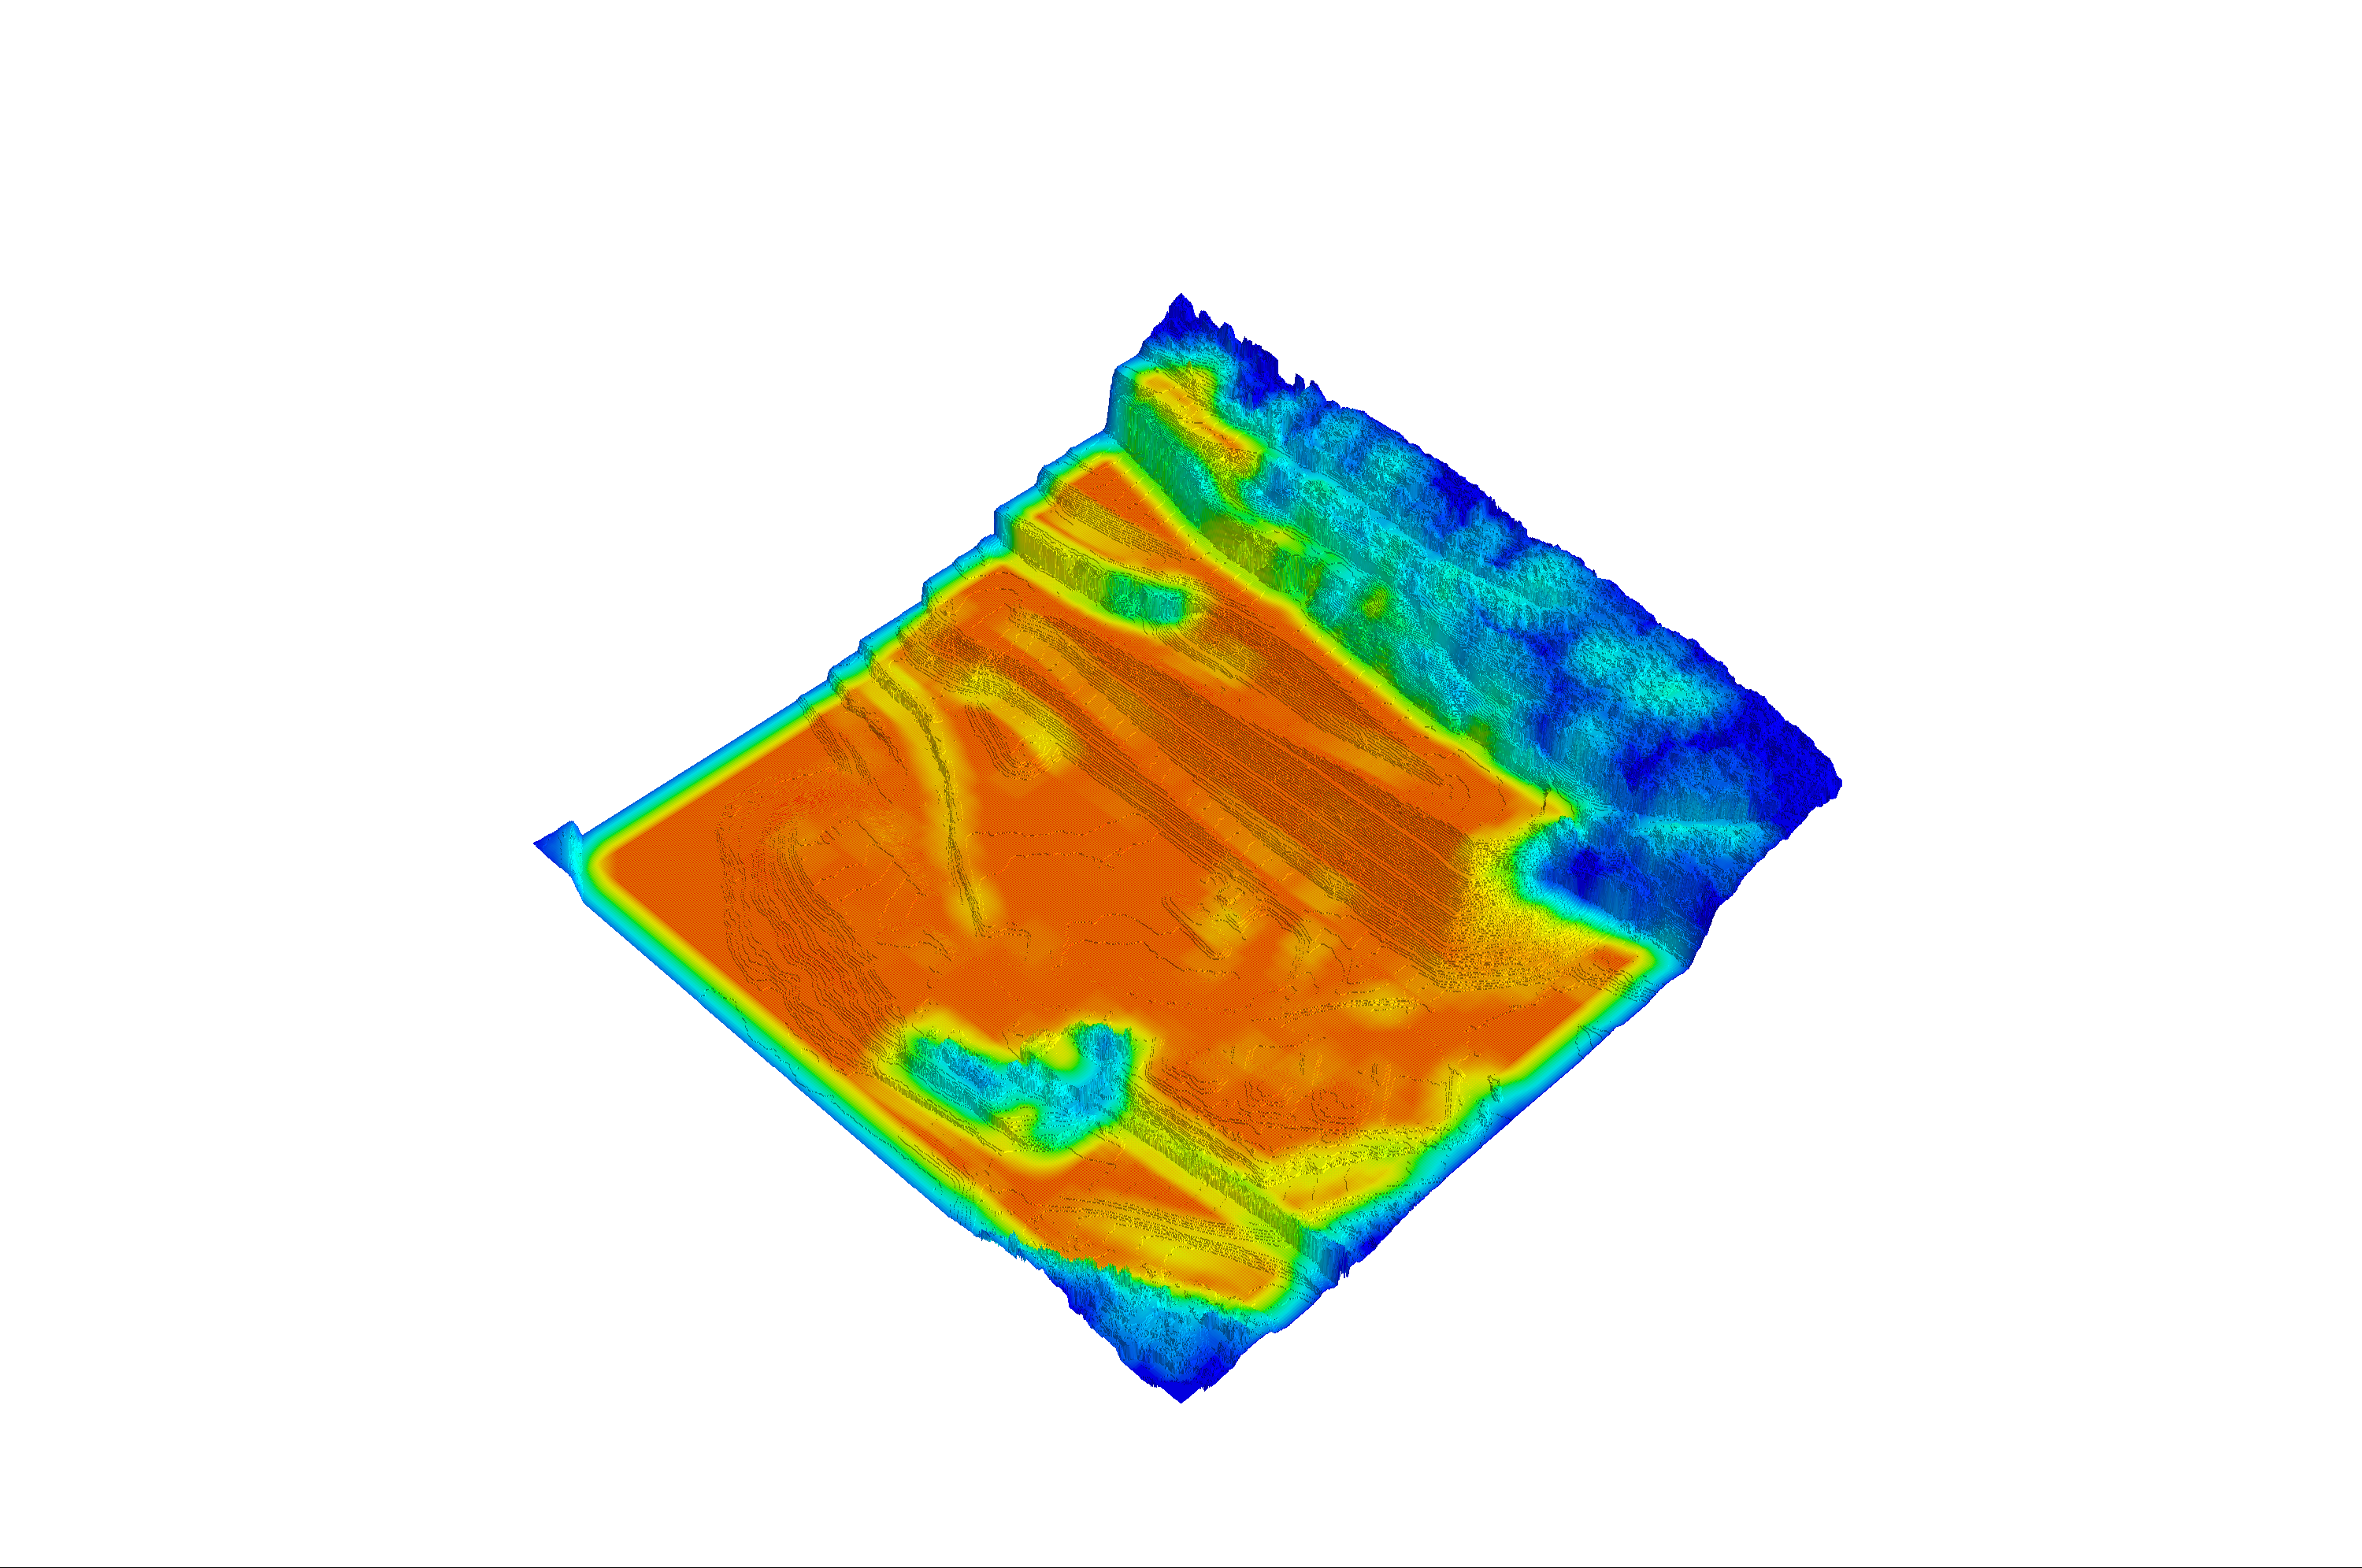
\includegraphics[width=\linewidth]{../img/4/traversability/quarry/180.png}  
\end{subfigure}

\caption{Traversability probability on the Quarry map for different Krock's rotation. The values are obstained by sliding a window on the map to create the patches to get the predictions from the model.}
\end{figure}
\todo[inline]{need to add arrows}
We can start our discussion by commenting the first image, Krock moving from bottom to top. Correctly, all the flat regions were label with high confidence as traversable, expecially the lower part of the map. There are two interesting regions, the bumps on the bottom right corner and the slopes. The following images higlights this two details
\todo[inline]{add images}
The slopes traversability is depends on the orientation. When the robot is moving up-hill, the propability is low while when it is going down those patches are completely traversable. Also, we the robot is moving from left to right and right to left it is able to traverse the slopes since the inclination is not too big to make the robot fall. 

For completeness, more images follow with their traversability probability.
\todo[inline]{add images of bars, arcs rocks}

\end{document}
% \documentclass[../document.tex]{subfiles}
\begin{document}
\todo[inline]{This chapter is under development!}
\chapter{Interpretability}
\label{chap: interpretability}
In this section, we will evaluate the model's prediction to better understand it. We will find if there are any features in the patches that can confuse it and if the model's output is robust.
First, we will show how the model learn to correctly separate the features from the two clases, then we will introduce on technique used to highlight the region of the input image that contribute the most to the model predictions. Then, we will use it on the data from the \emph{Quarry} test set to find out the patches were the model fails and analyze them.

Later, we will work with custom created patches with different features, walls, bumps, etc, to test the robustness of the model by comparing its predictions to the real data gathered from the simulator.


\subsection{Features separability}
In general, convolutional neural network learns to encode images by applying filters of increasing sizes at each layer. Usually, the first layers learn basic features, such us edges, while the final one encodes complex shapes. Those final informations are combined and mapped to the correct classes by one or more fully connected. For example, the following image was generated by plotting the learned features for different categories at different layers by 
Lee et al. \cite{deepbelief}
\begin{figure}[H]
    \centering
    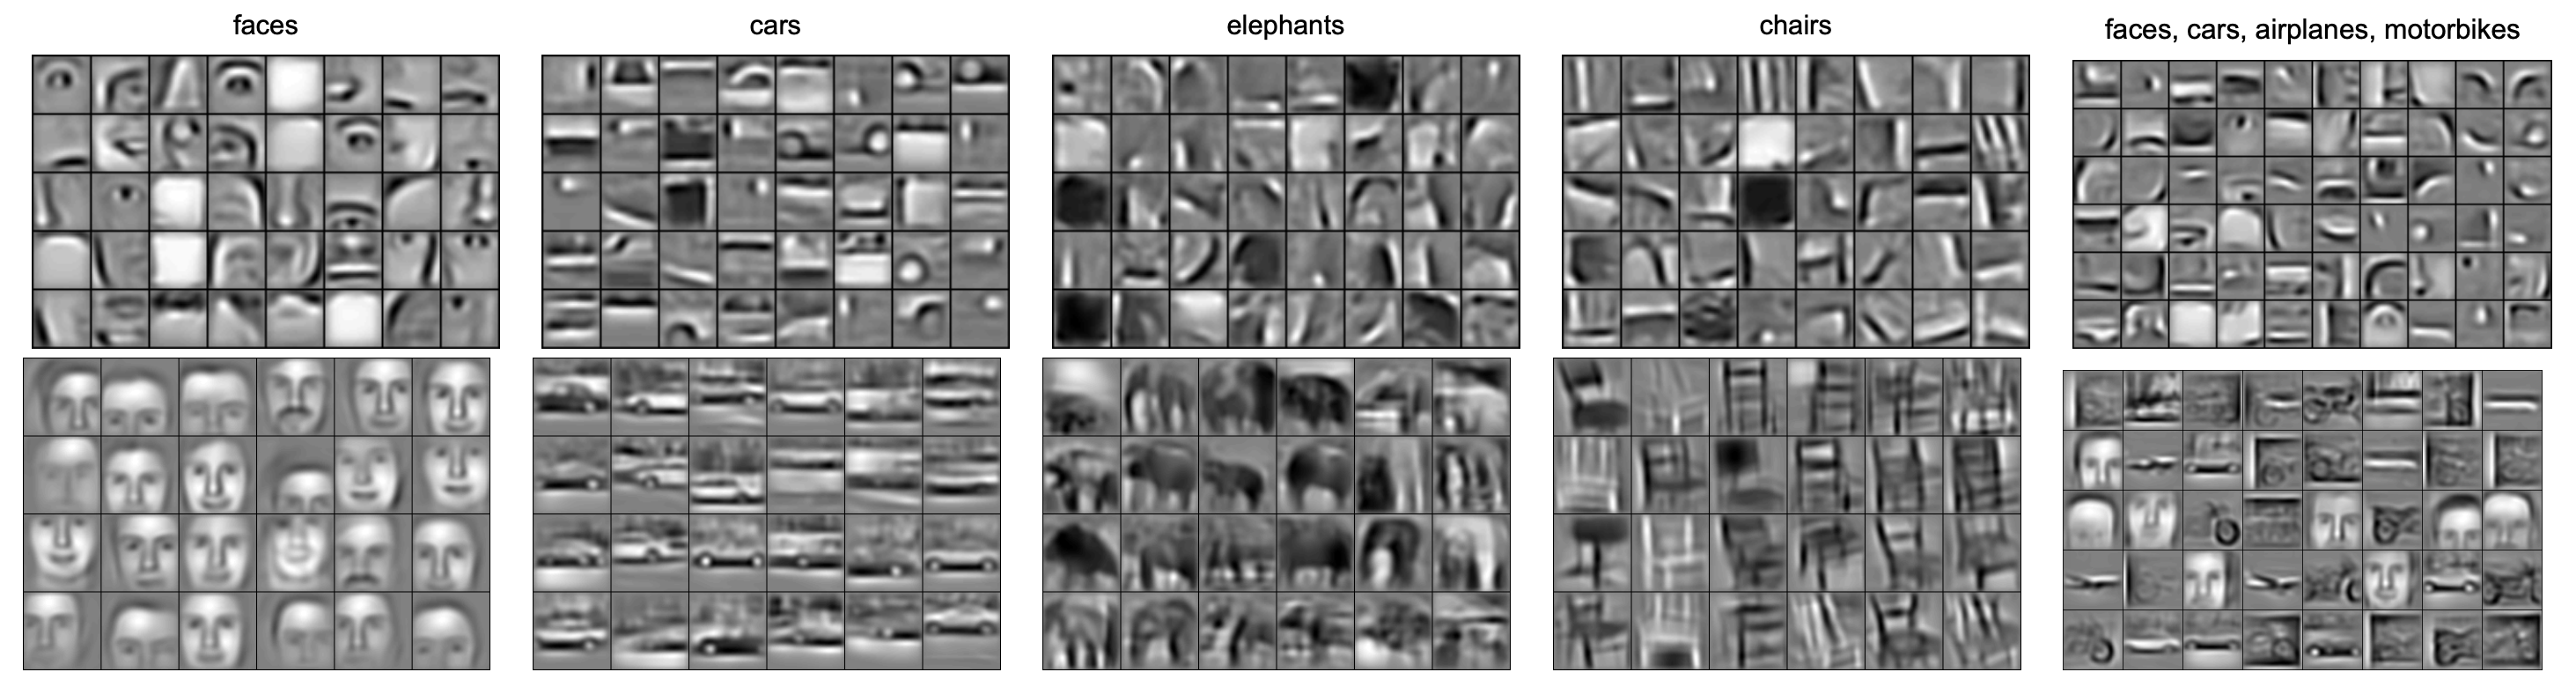
\includegraphics[width=\linewidth]{../img/5/deep_belief.png}
    \caption{Figure from Lee et al. \cite{deepbelief} paper where they shown for different classes the low-level features (up) and the high-level features (down) learned by a convolution neural network.}
\end{figure}
So, a correctly trained network should be able to separate those features based on predicted classes. Intuitivelly, given two classes $\mathcal{A}$ and $\mathcal{B}$, for example \emph{cat} and \emph{dog}, the high-level features for each class should not be the same, otherwise the model may output a wrong prediction since the same feature is maped to different classes. 
Thus, visualizing the inputs features vectors against each class can give a good quality estimation of the model since highly separable features yield a correct learning procedure.  Our model, MicroResNet, has a last convolution layer's features size of $[128, 3, 3 ]$. Since visualize a $128$ dimension vector is impossible, we reduce its dimension to $2$ by applying Principle Anyalisis Component (PCA) \cite{pca}. 

\subsection{Train set}
The following figures shows the features of $11$K images sampled from the train set label with their classes, \emph{traversable} and \emph{not traversable}.
\begin{figure}[H]
    \centering
    \begin{subfigure}[b]{1\textwidth}
        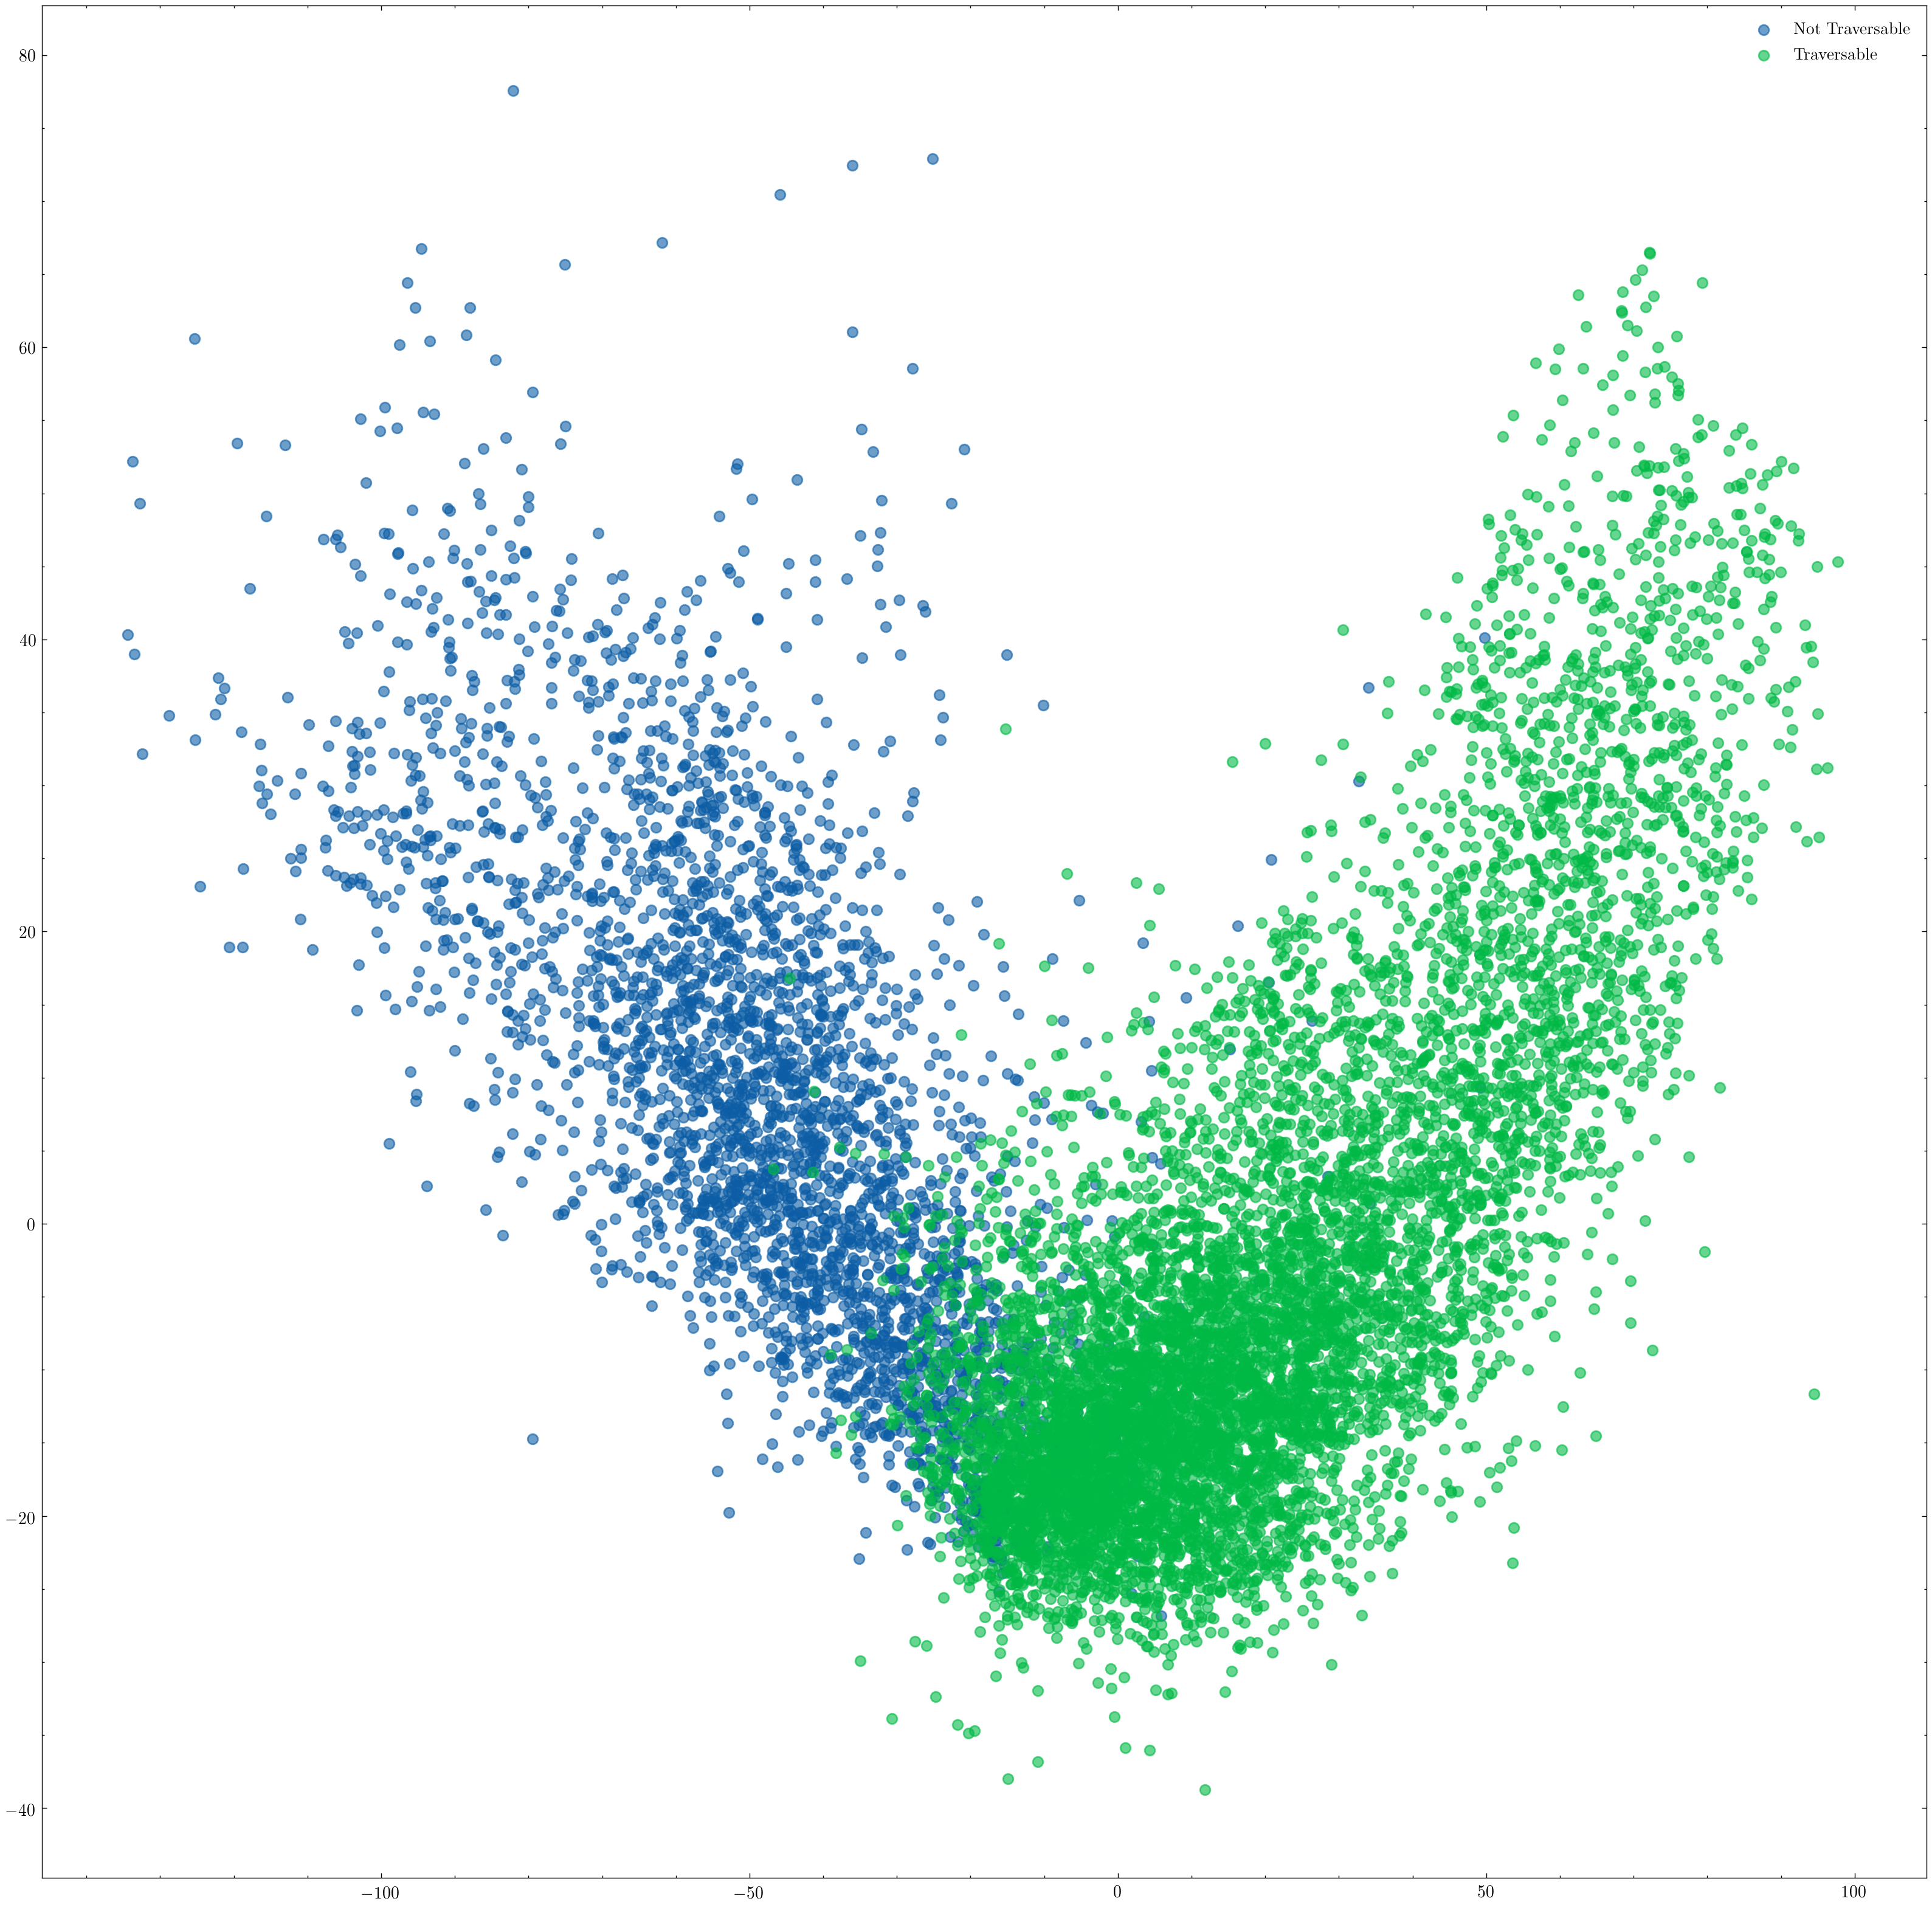
\includegraphics[width=\linewidth]{../img/5/pca/pca.png}
    \end{subfigure}
    \begin{subfigure}[b]{0.48\textwidth}
        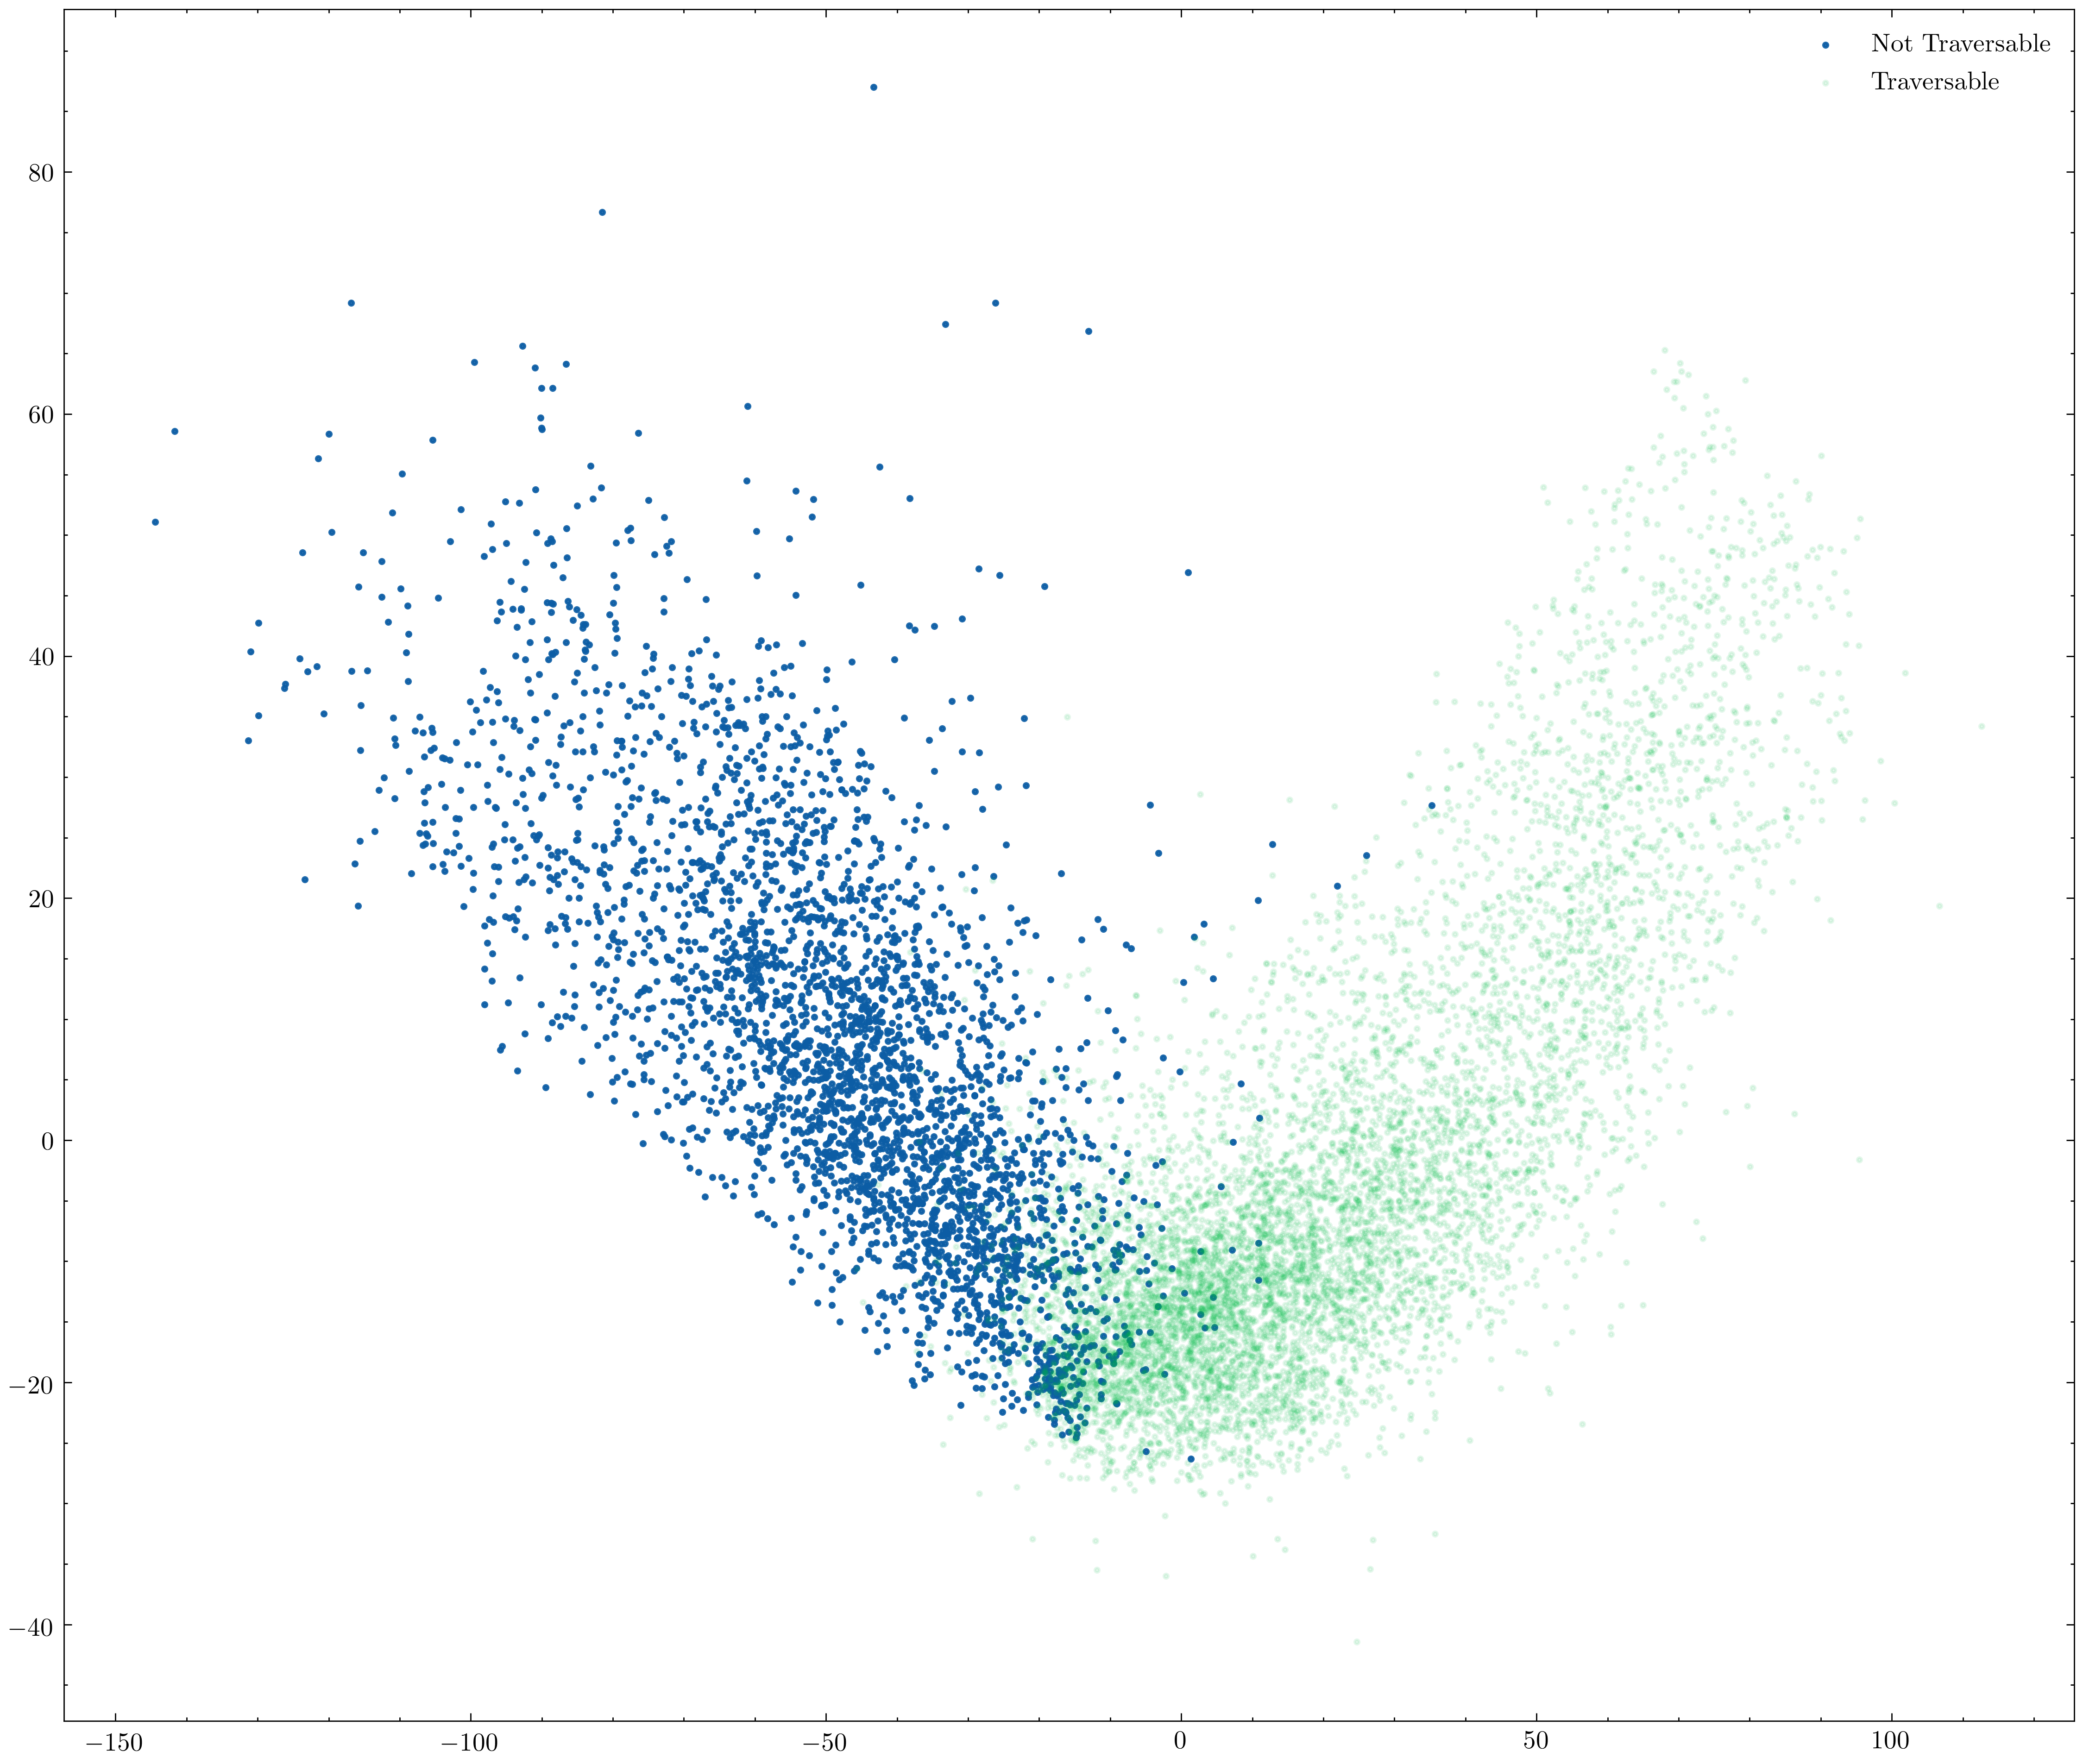
\includegraphics[width=\linewidth]{../img/5/pca/pca-0.png}
        \caption{Not Traversable}
    \end{subfigure}
    \begin{subfigure}[b]{0.48\textwidth}
        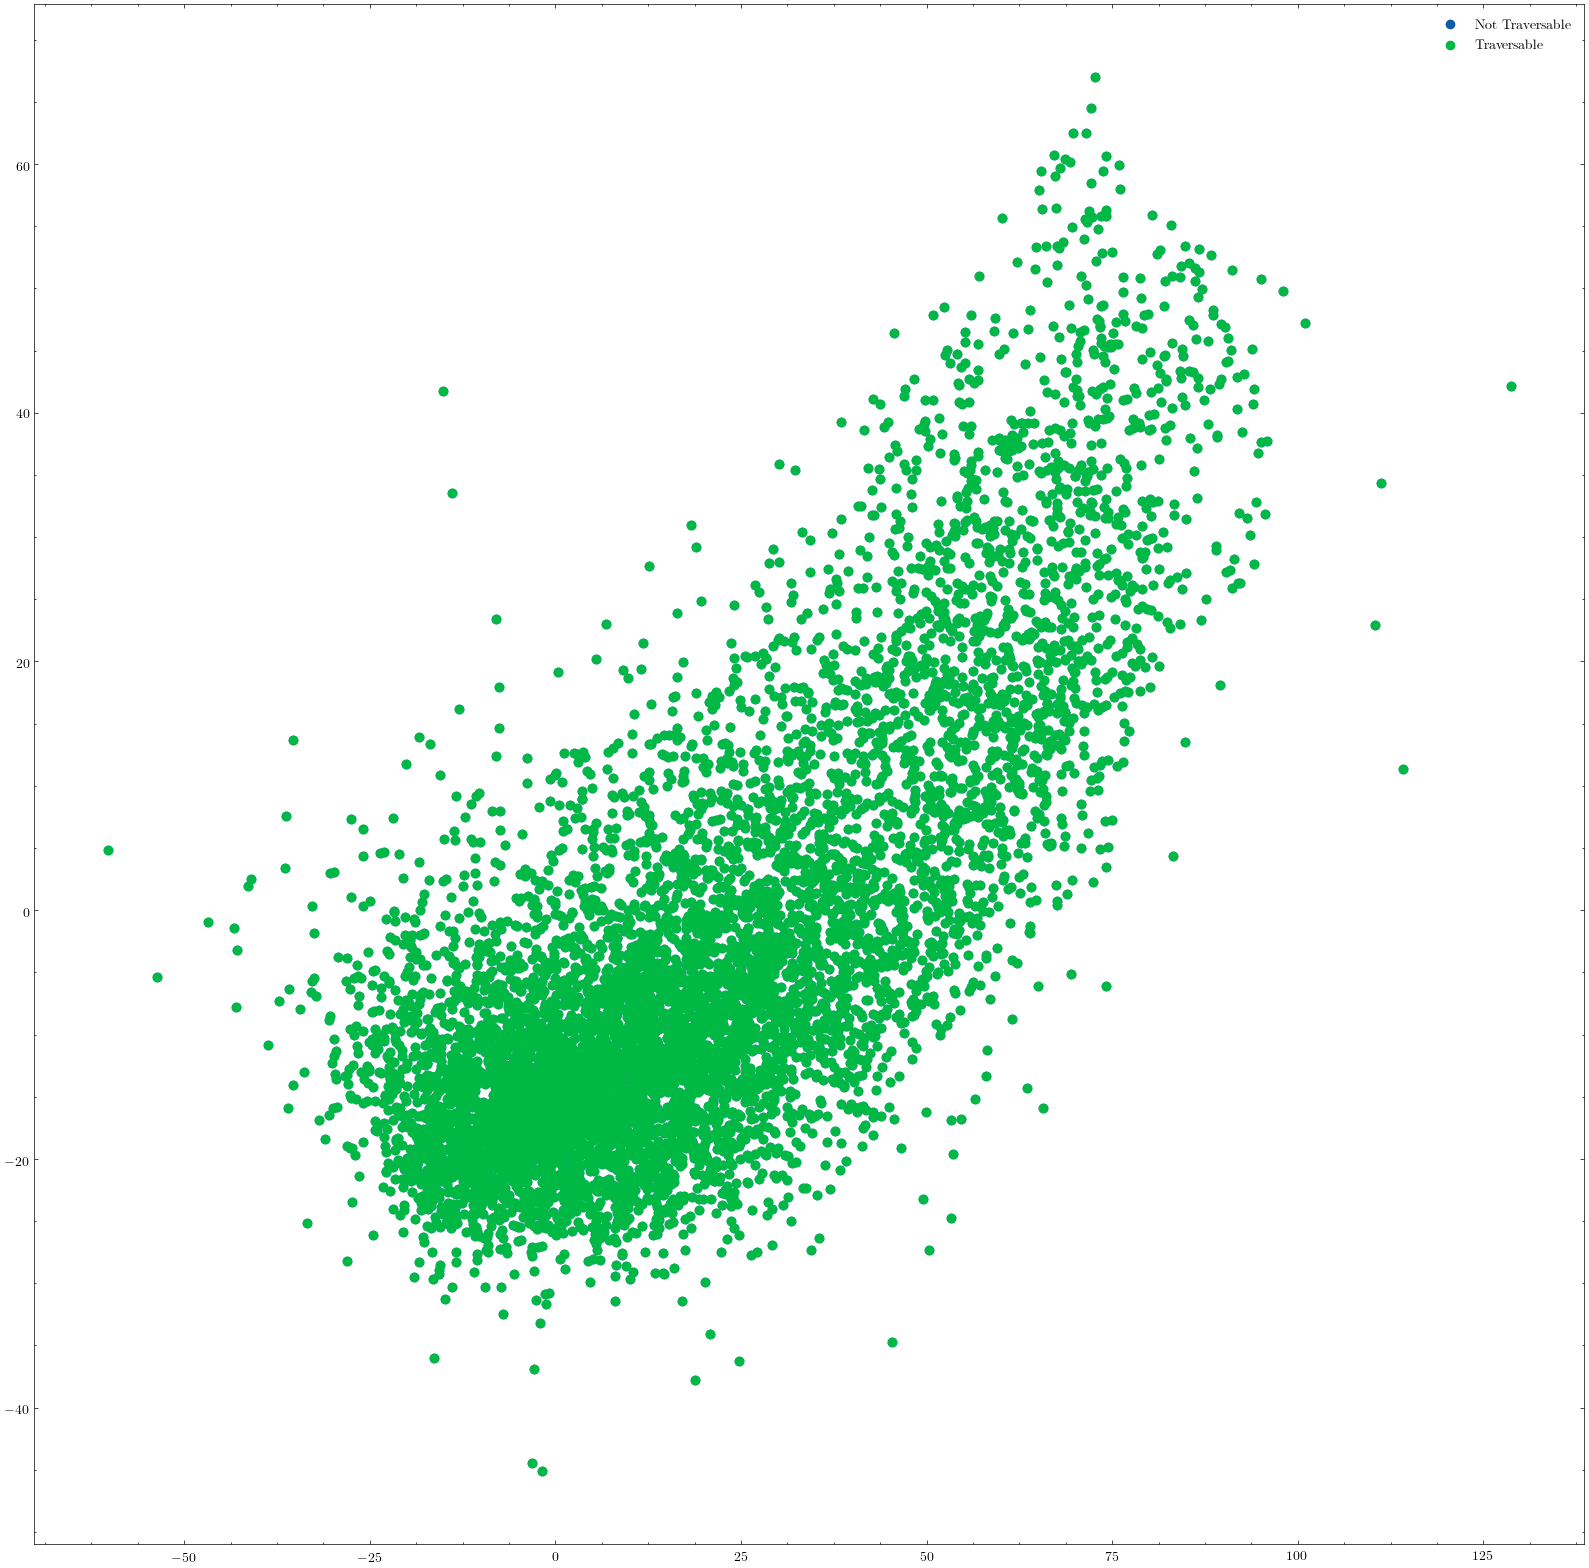
\includegraphics[width=\linewidth]{../img/5/pca/pca-1.png}
        \caption{Traversable}
    \end{subfigure}
\caption{Principal Component Analysis on the features space computed using the features from the last convolutional layers on the train dataset.}
\end{figure}
We can clearly distinguish two main clusters based on the labels, one on the left and one of the right. Those points are easily separable, even by human eyes, meaning that the model was able to learn meaning features from the dataset. Moreover, if we plot the density center, we can see that most of the samples per class are not very close.

\begin{figure}[H]
    \begin{subfigure}[b]{0.48\textwidth}
        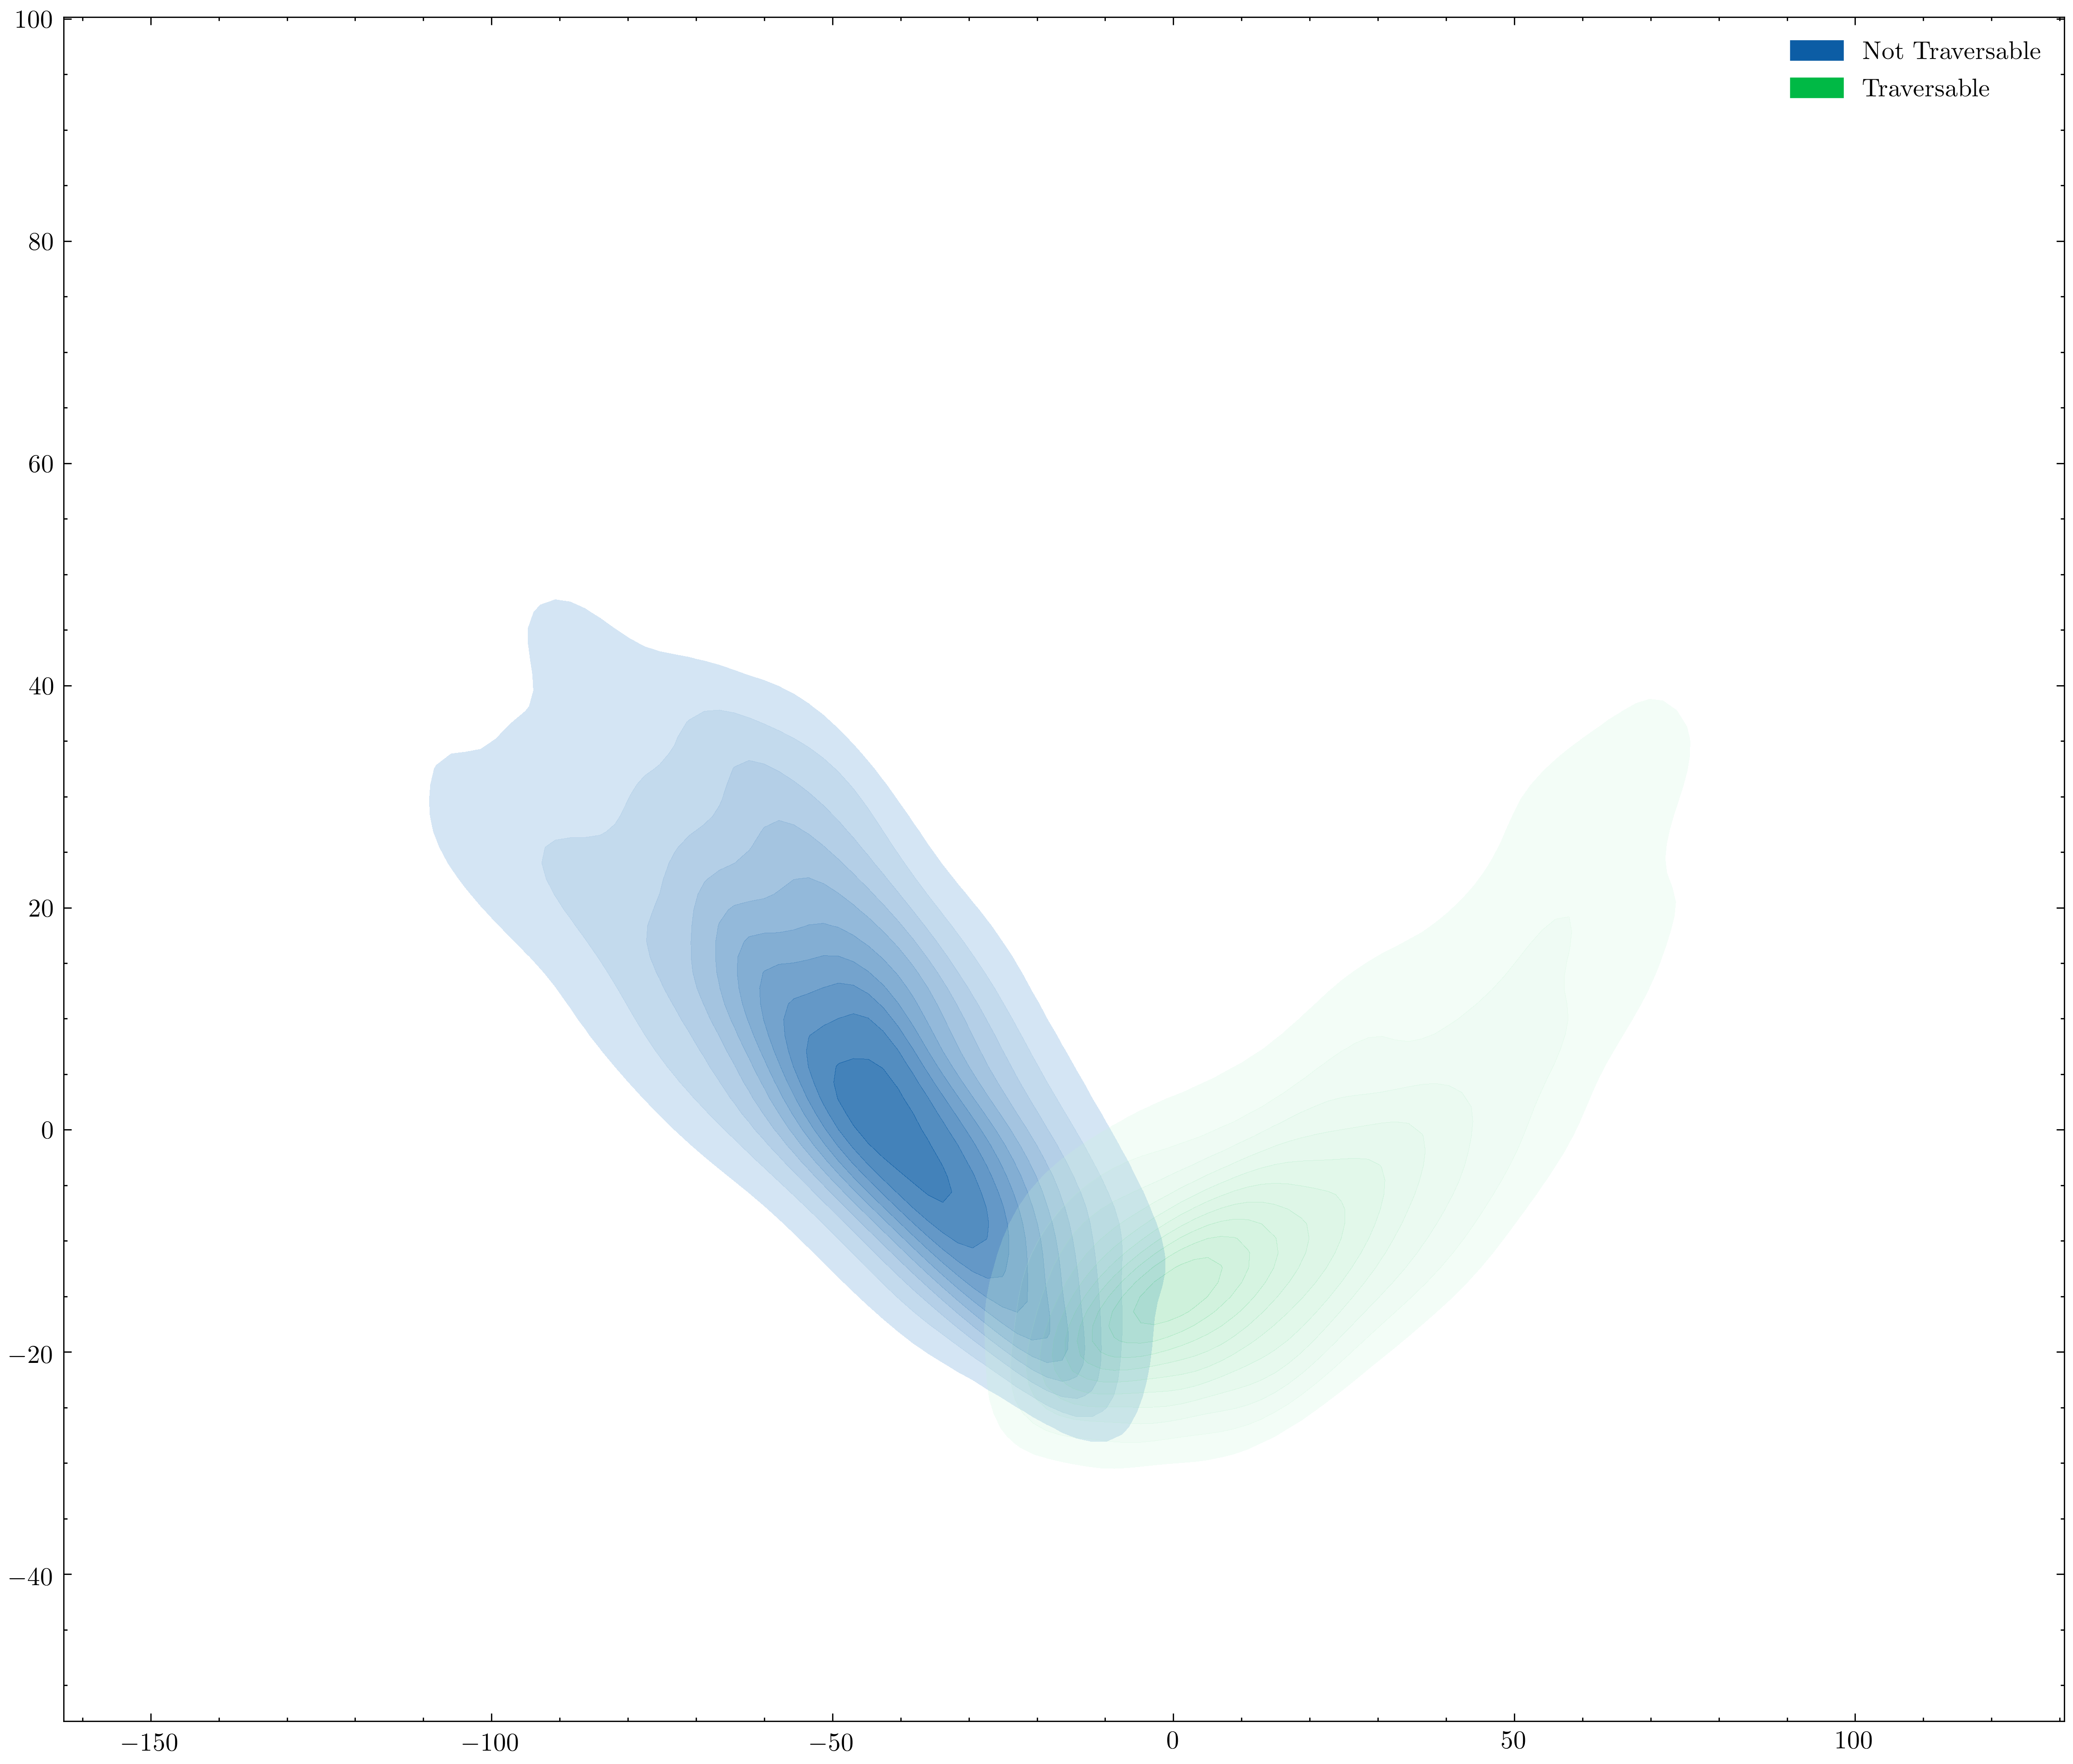
\includegraphics[width=\linewidth]{../img/5/pca/pca-0-density.png}
        \caption{Not Traversable}
    \end{subfigure}
    \begin{subfigure}[b]{0.48\textwidth}
        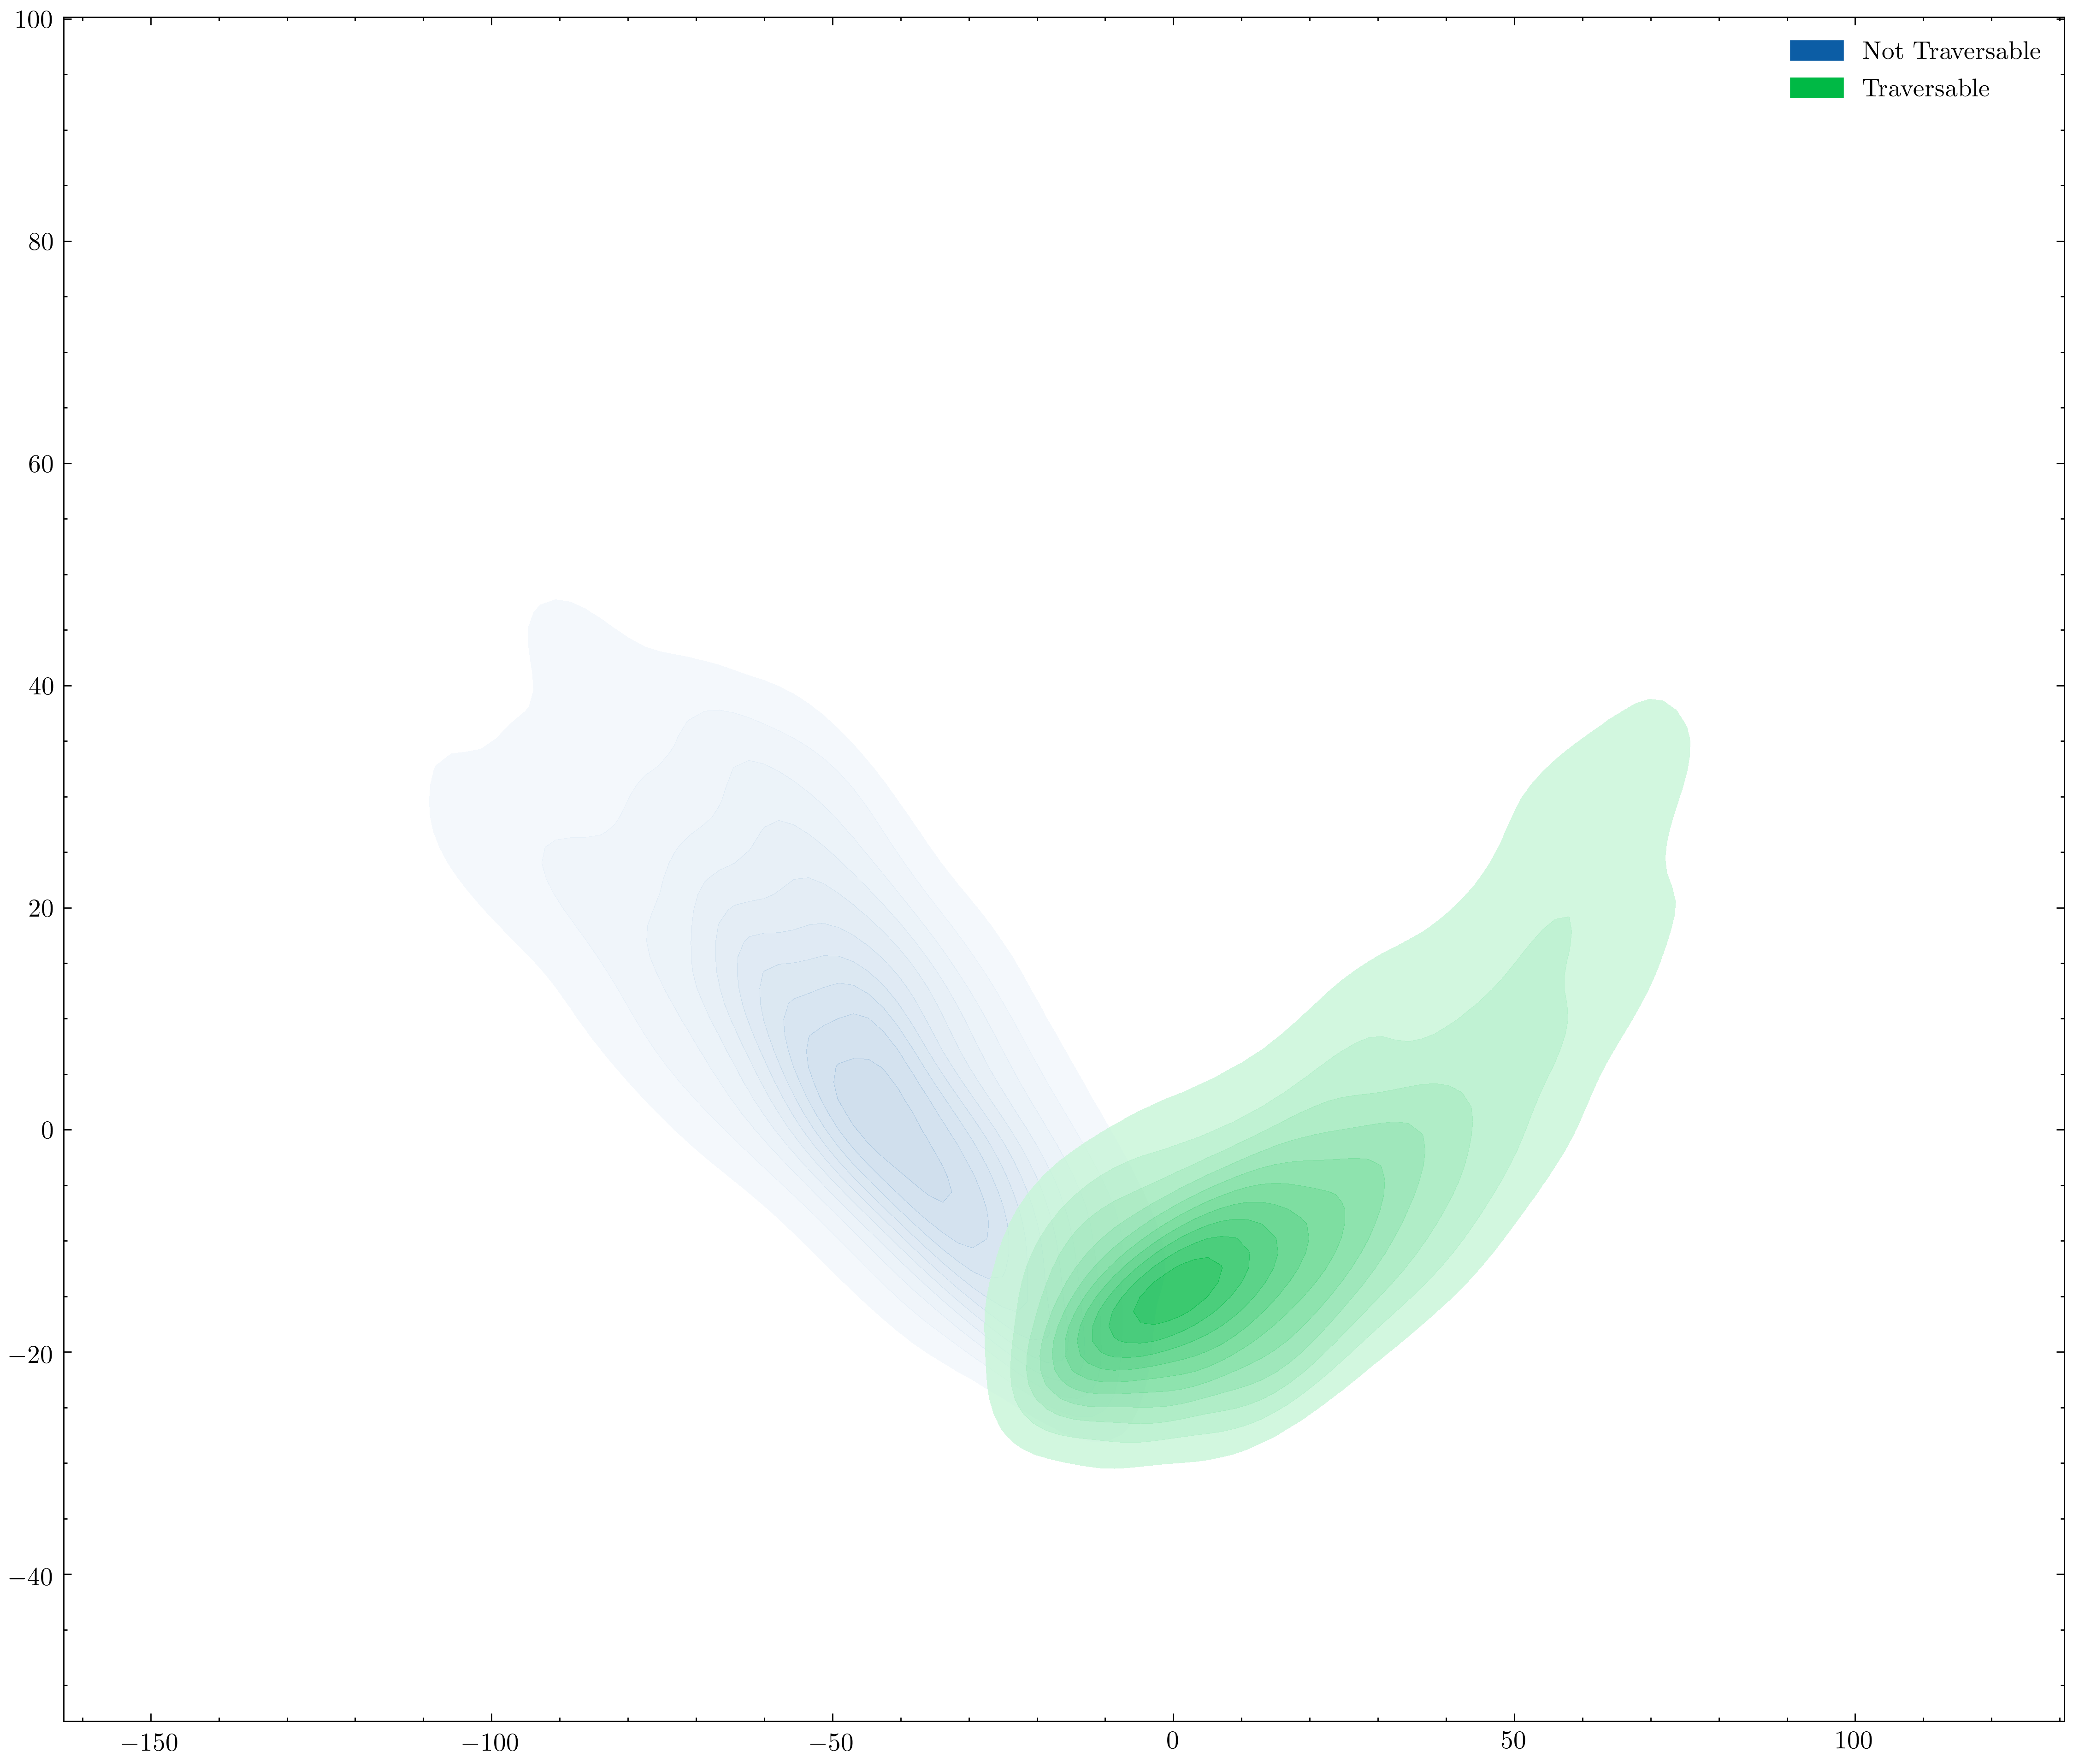
\includegraphics[width=\linewidth]{../img/5/pca/pca-1-density.png}
        \caption{Traversable}
    \end{subfigure}
    \caption{Density plot for the points sampled from the train dataset in the features space. The centers of the cluster are not overlapping yielding a good separability and a correct learning.}
    \end{figure}
We can also identify patches based on their position in the features space, for example, the points on the top left cloud, are patches with walls or big bumps. On the other hand, the hardest patch to classify, or in separate in the features space, are the ones in the middle. Those are the patches with a relatively flat ground and small obstacles. One advatange of this procedure is that intrinsically, similar patches will be close to eachother helping to identify clusters of inputs. We decided to not show all images on the same plot to avoid overcrowing the image. Instead, we clusted the points using K-Means with $k=200$ clusters and then we took the patch that corresponded to the center point in each cluster. In this way, even if we are showing only a few inputs, we included all the meaningfull features. The following image shows the result. 
\begin{figure}[H]
    \centering
    \begin{subfigure}[b]{1\textwidth}
        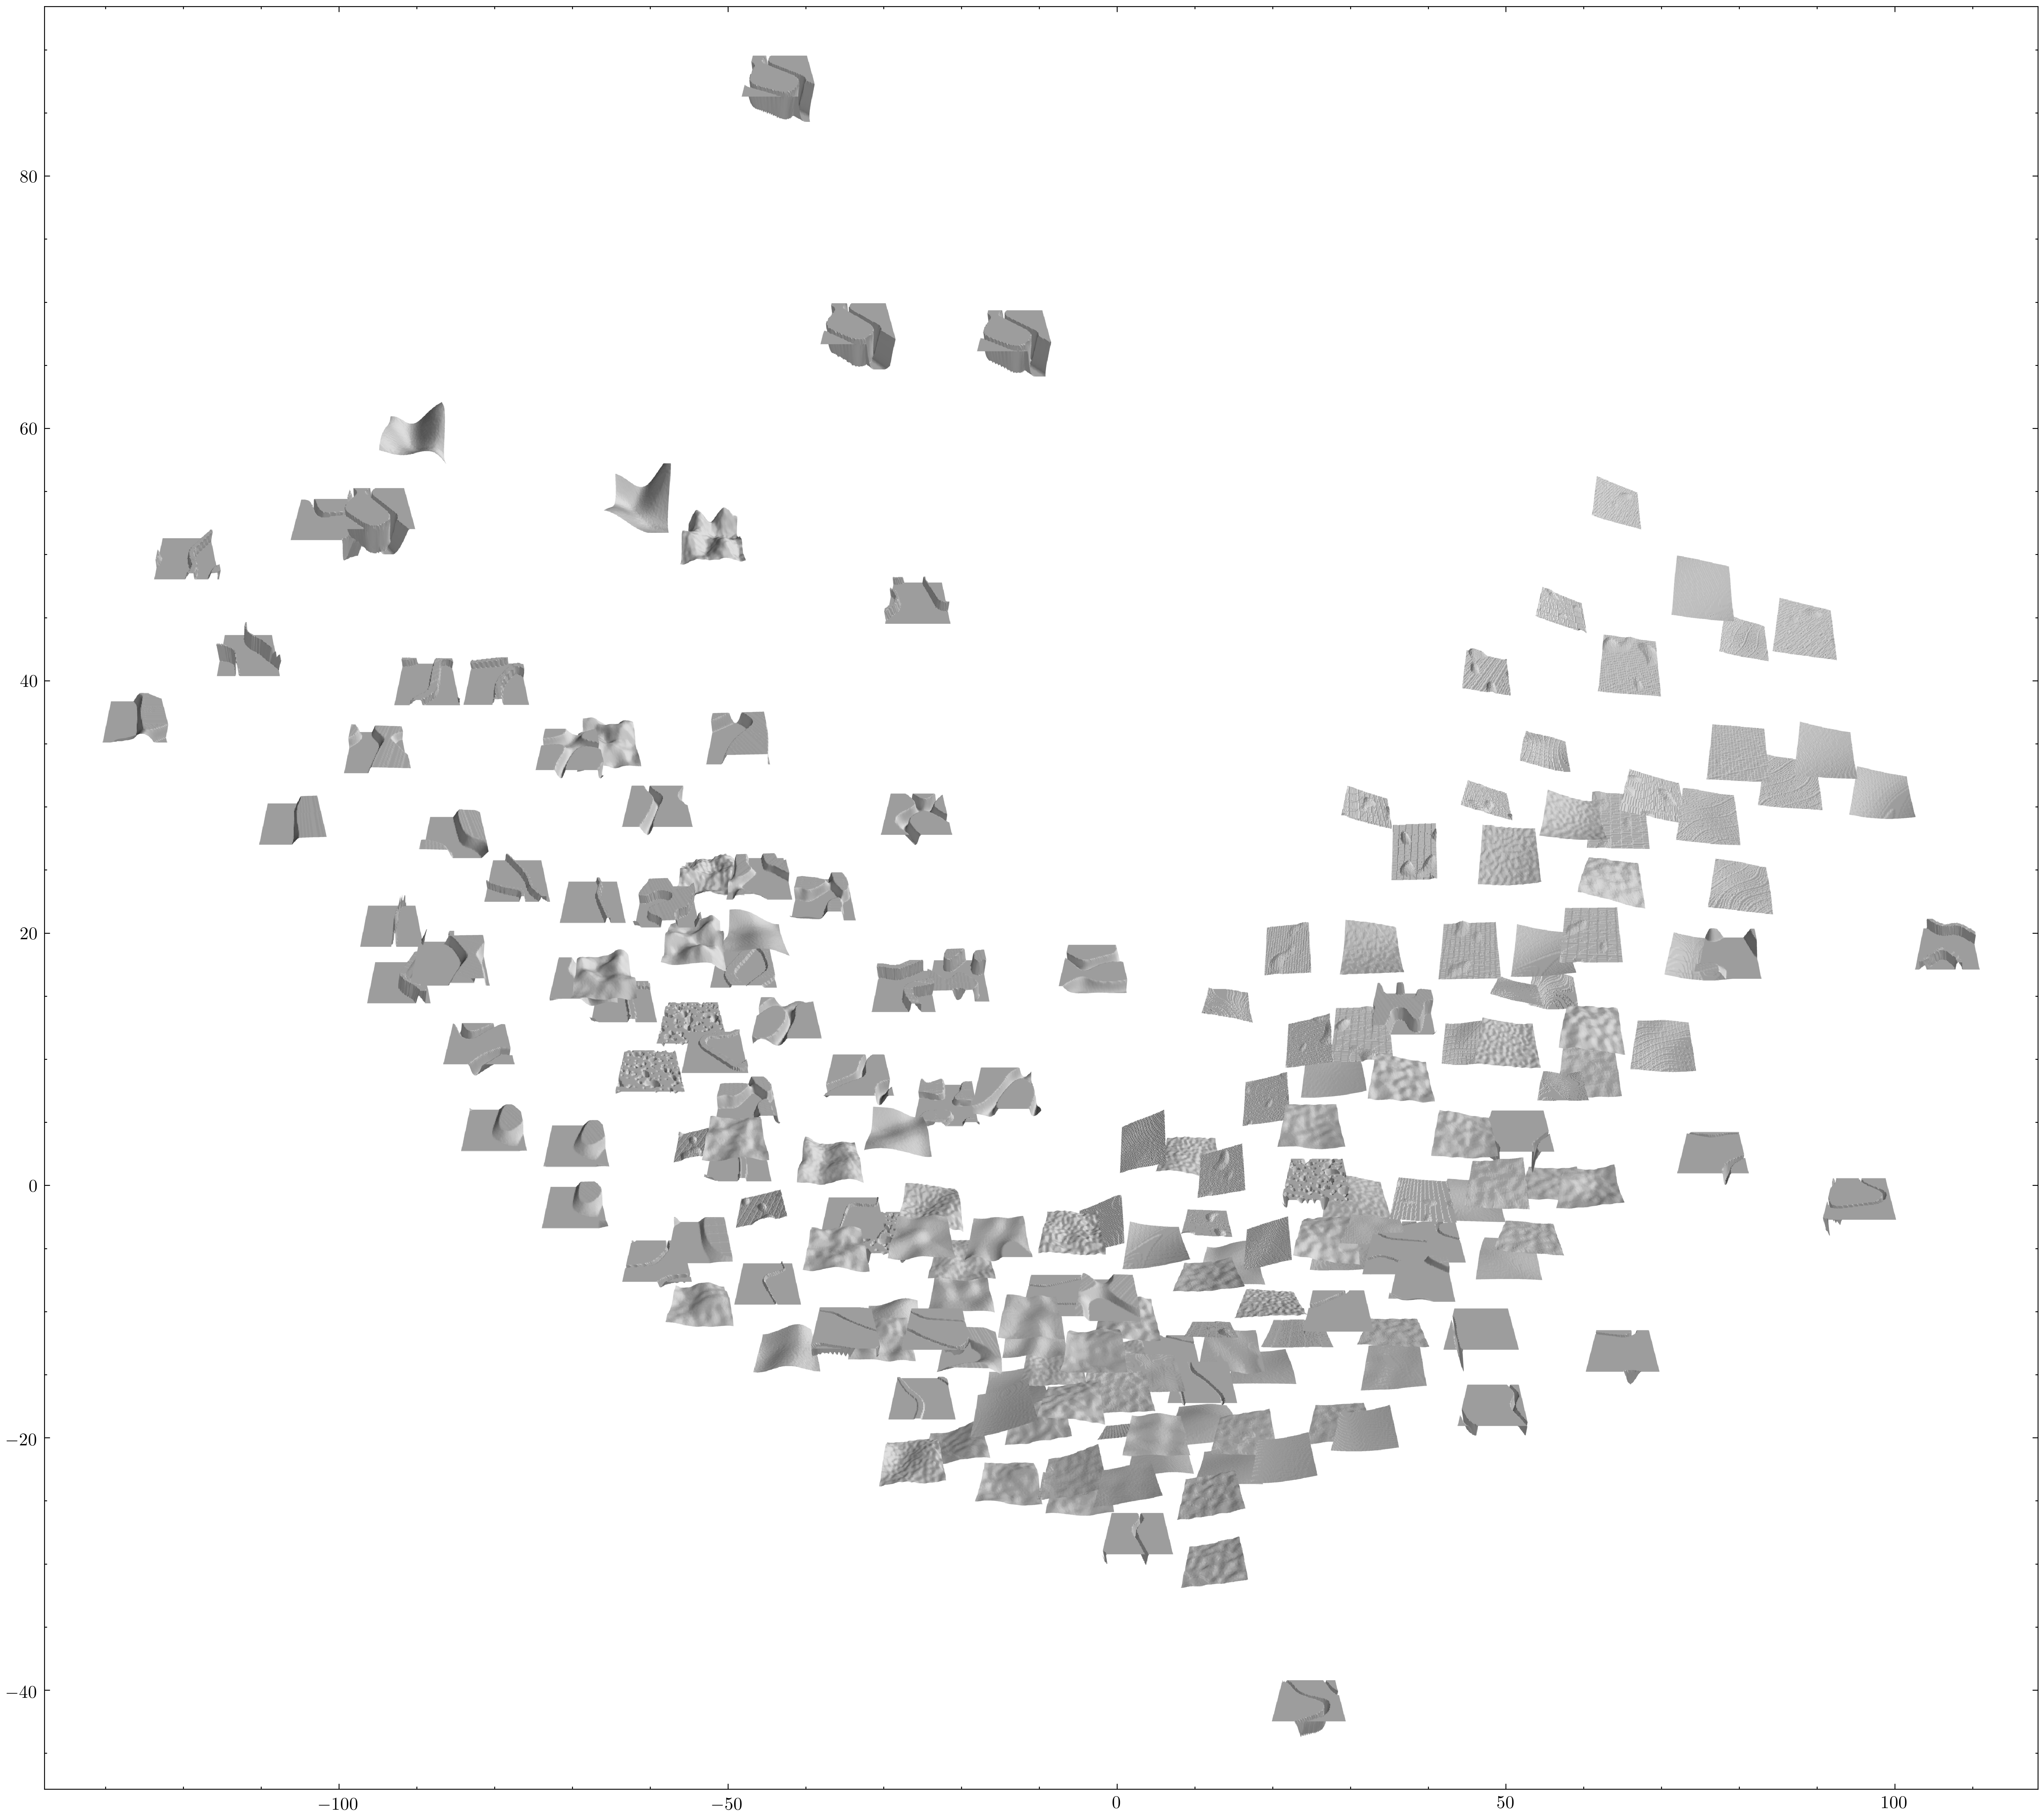
\includegraphics[width=\linewidth]{../img/5/pca/pca-patches-200.png}
    \end{subfigure}
    \caption{Patches that cooresponds to coordinates in the features space of the last convolutional layers on the train dataset. Similar grounds are close to each other.}
\end{figure}
Patches with similar features are close to eachother. On the left-top side, we can distinguish highgly non traversable patches with walls/bumps in front of the robot. Going down, we start to encoter patches with ligher obstacles. On the platoue, there are traversable patches with small obstacles such as light bumps. It is important to notice that those patches are the closest ones to the non traversable ones, meaning that those are the most harder inputs for the model to classify. Going up on the right side, we see some small steps. Finally, on the top, we find all the downhill patches, the easiest ones to traverse.

\subsection{Test set}
We can apply the same procedure to evaluate the test set. This dataset is harder and present challanging situation for the robot, so we expected some points to be mixedup.
\begin{figure}[H]
    \centering
    \begin{subfigure}[b]{1\textwidth}
        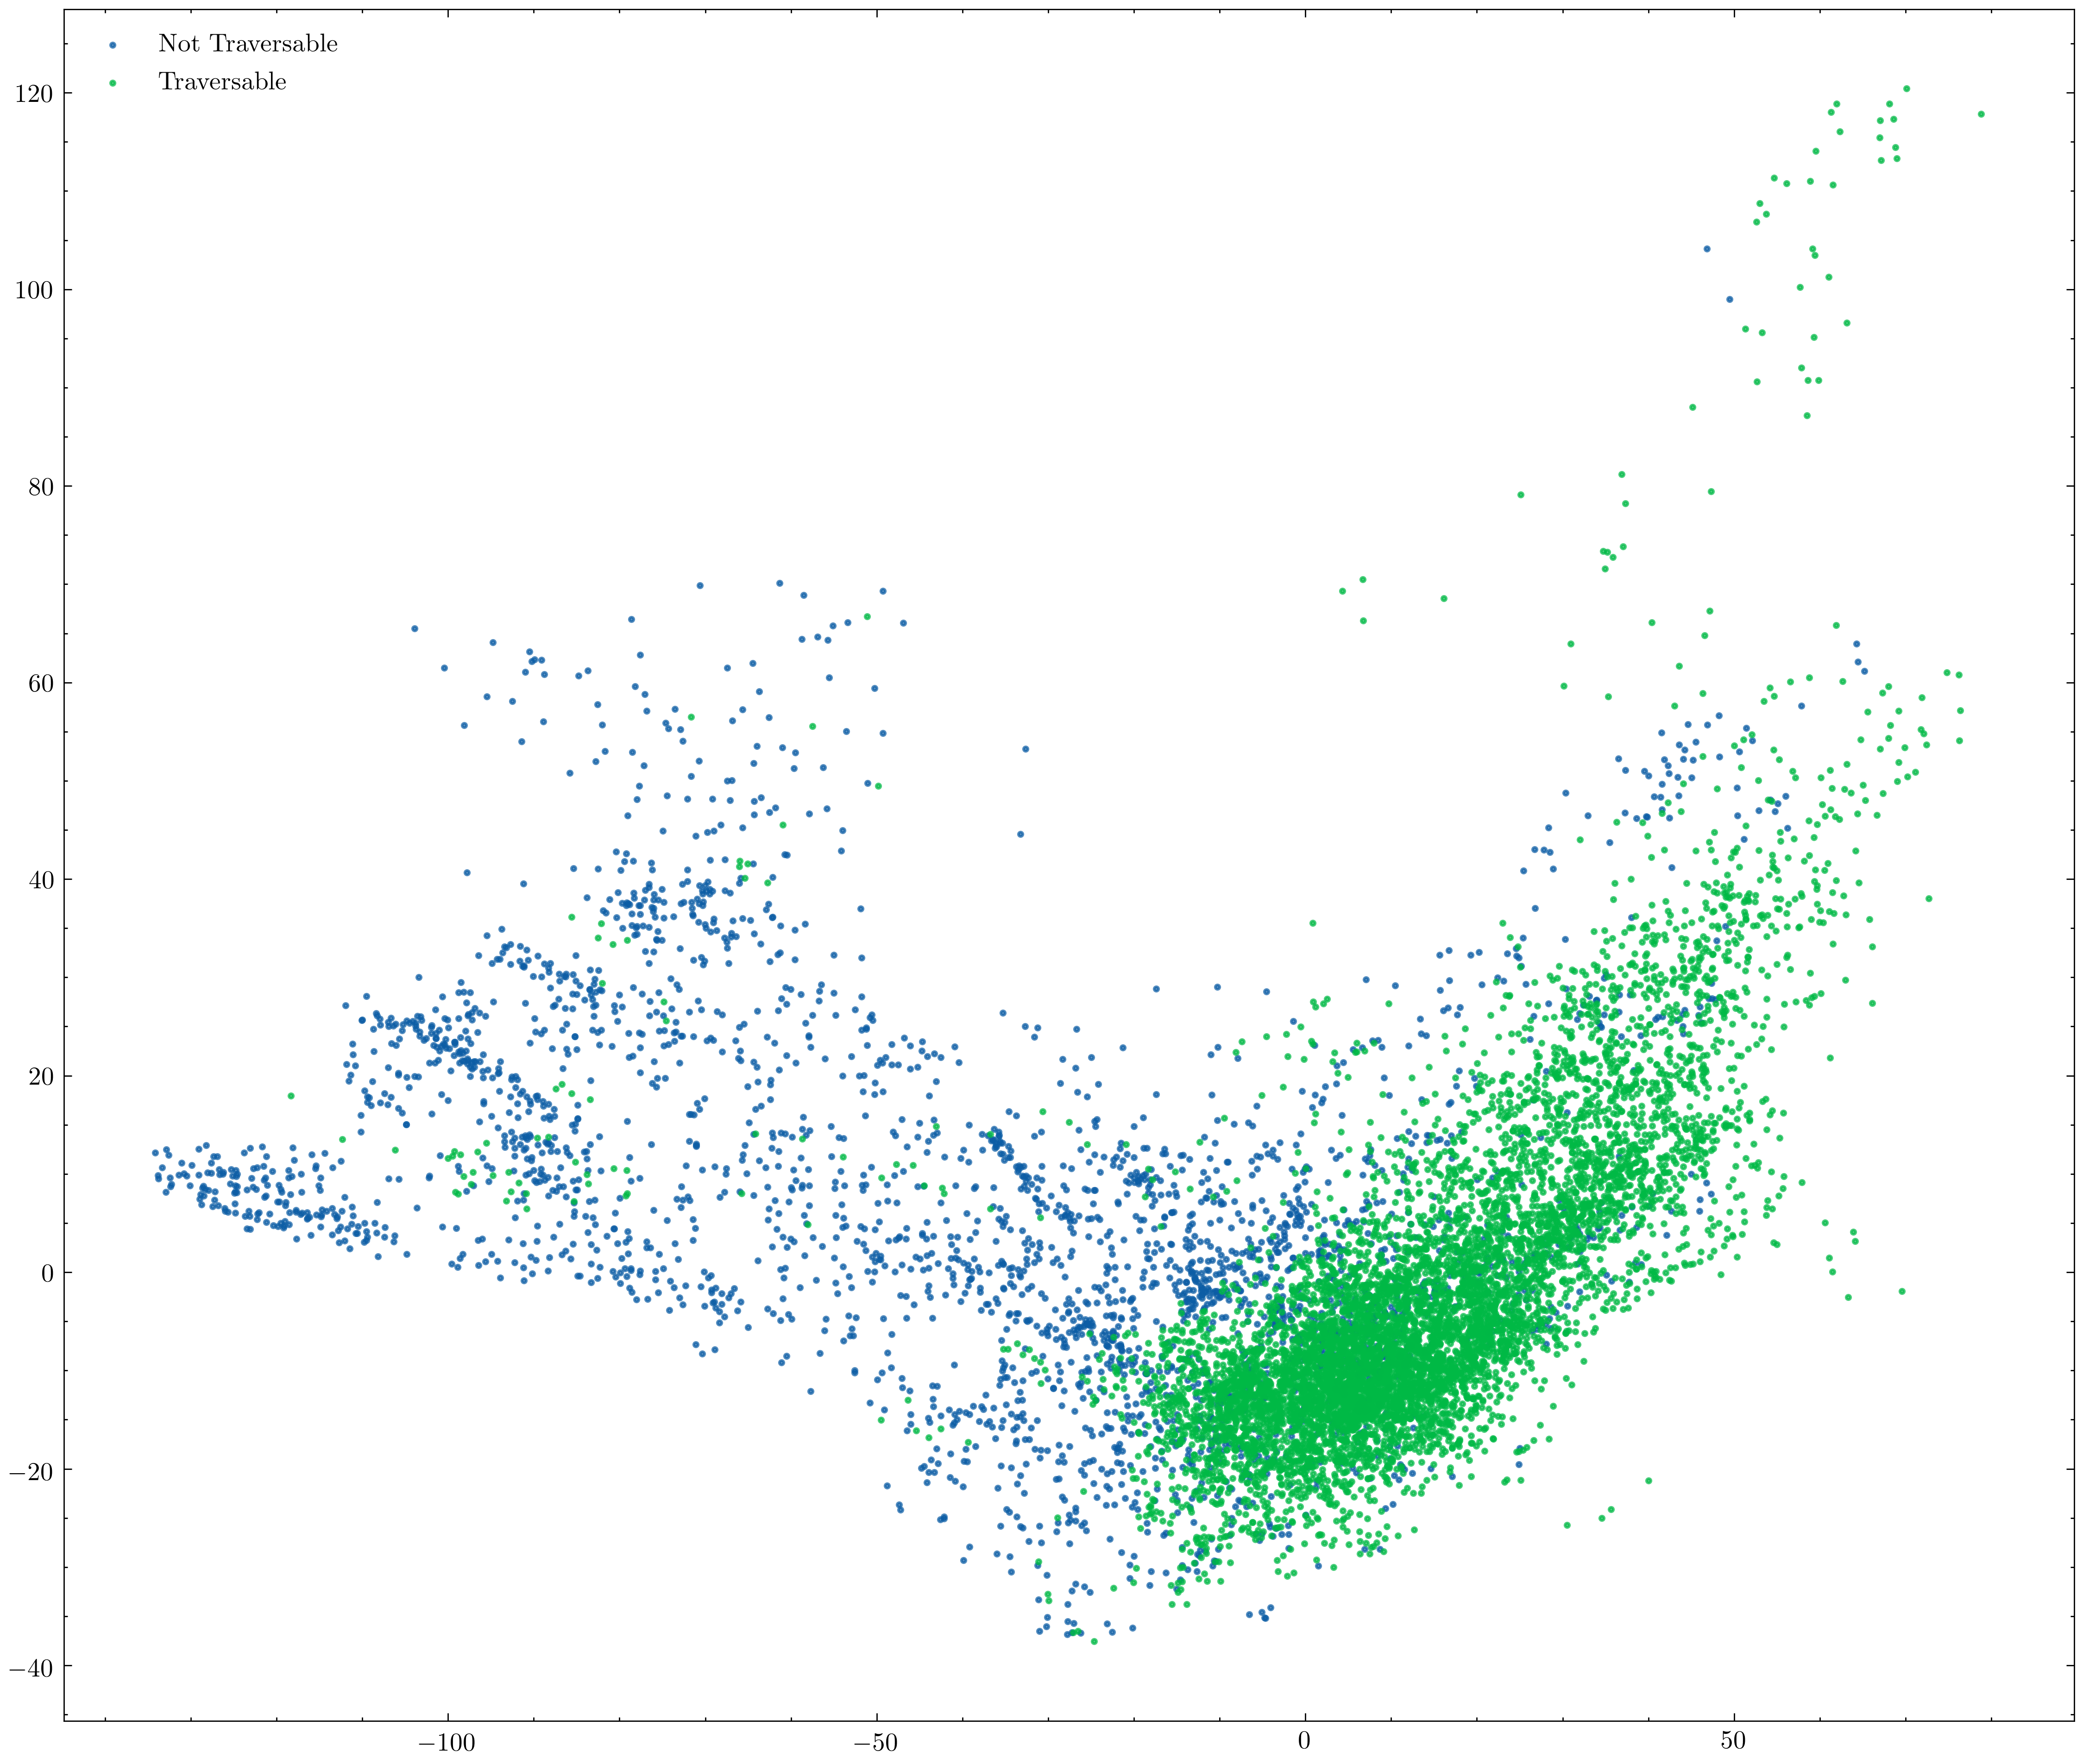
\includegraphics[width=\linewidth]{../img/5/pca/pca-test.png}
    \end{subfigure}
    \begin{subfigure}[b]{0.48\textwidth}
        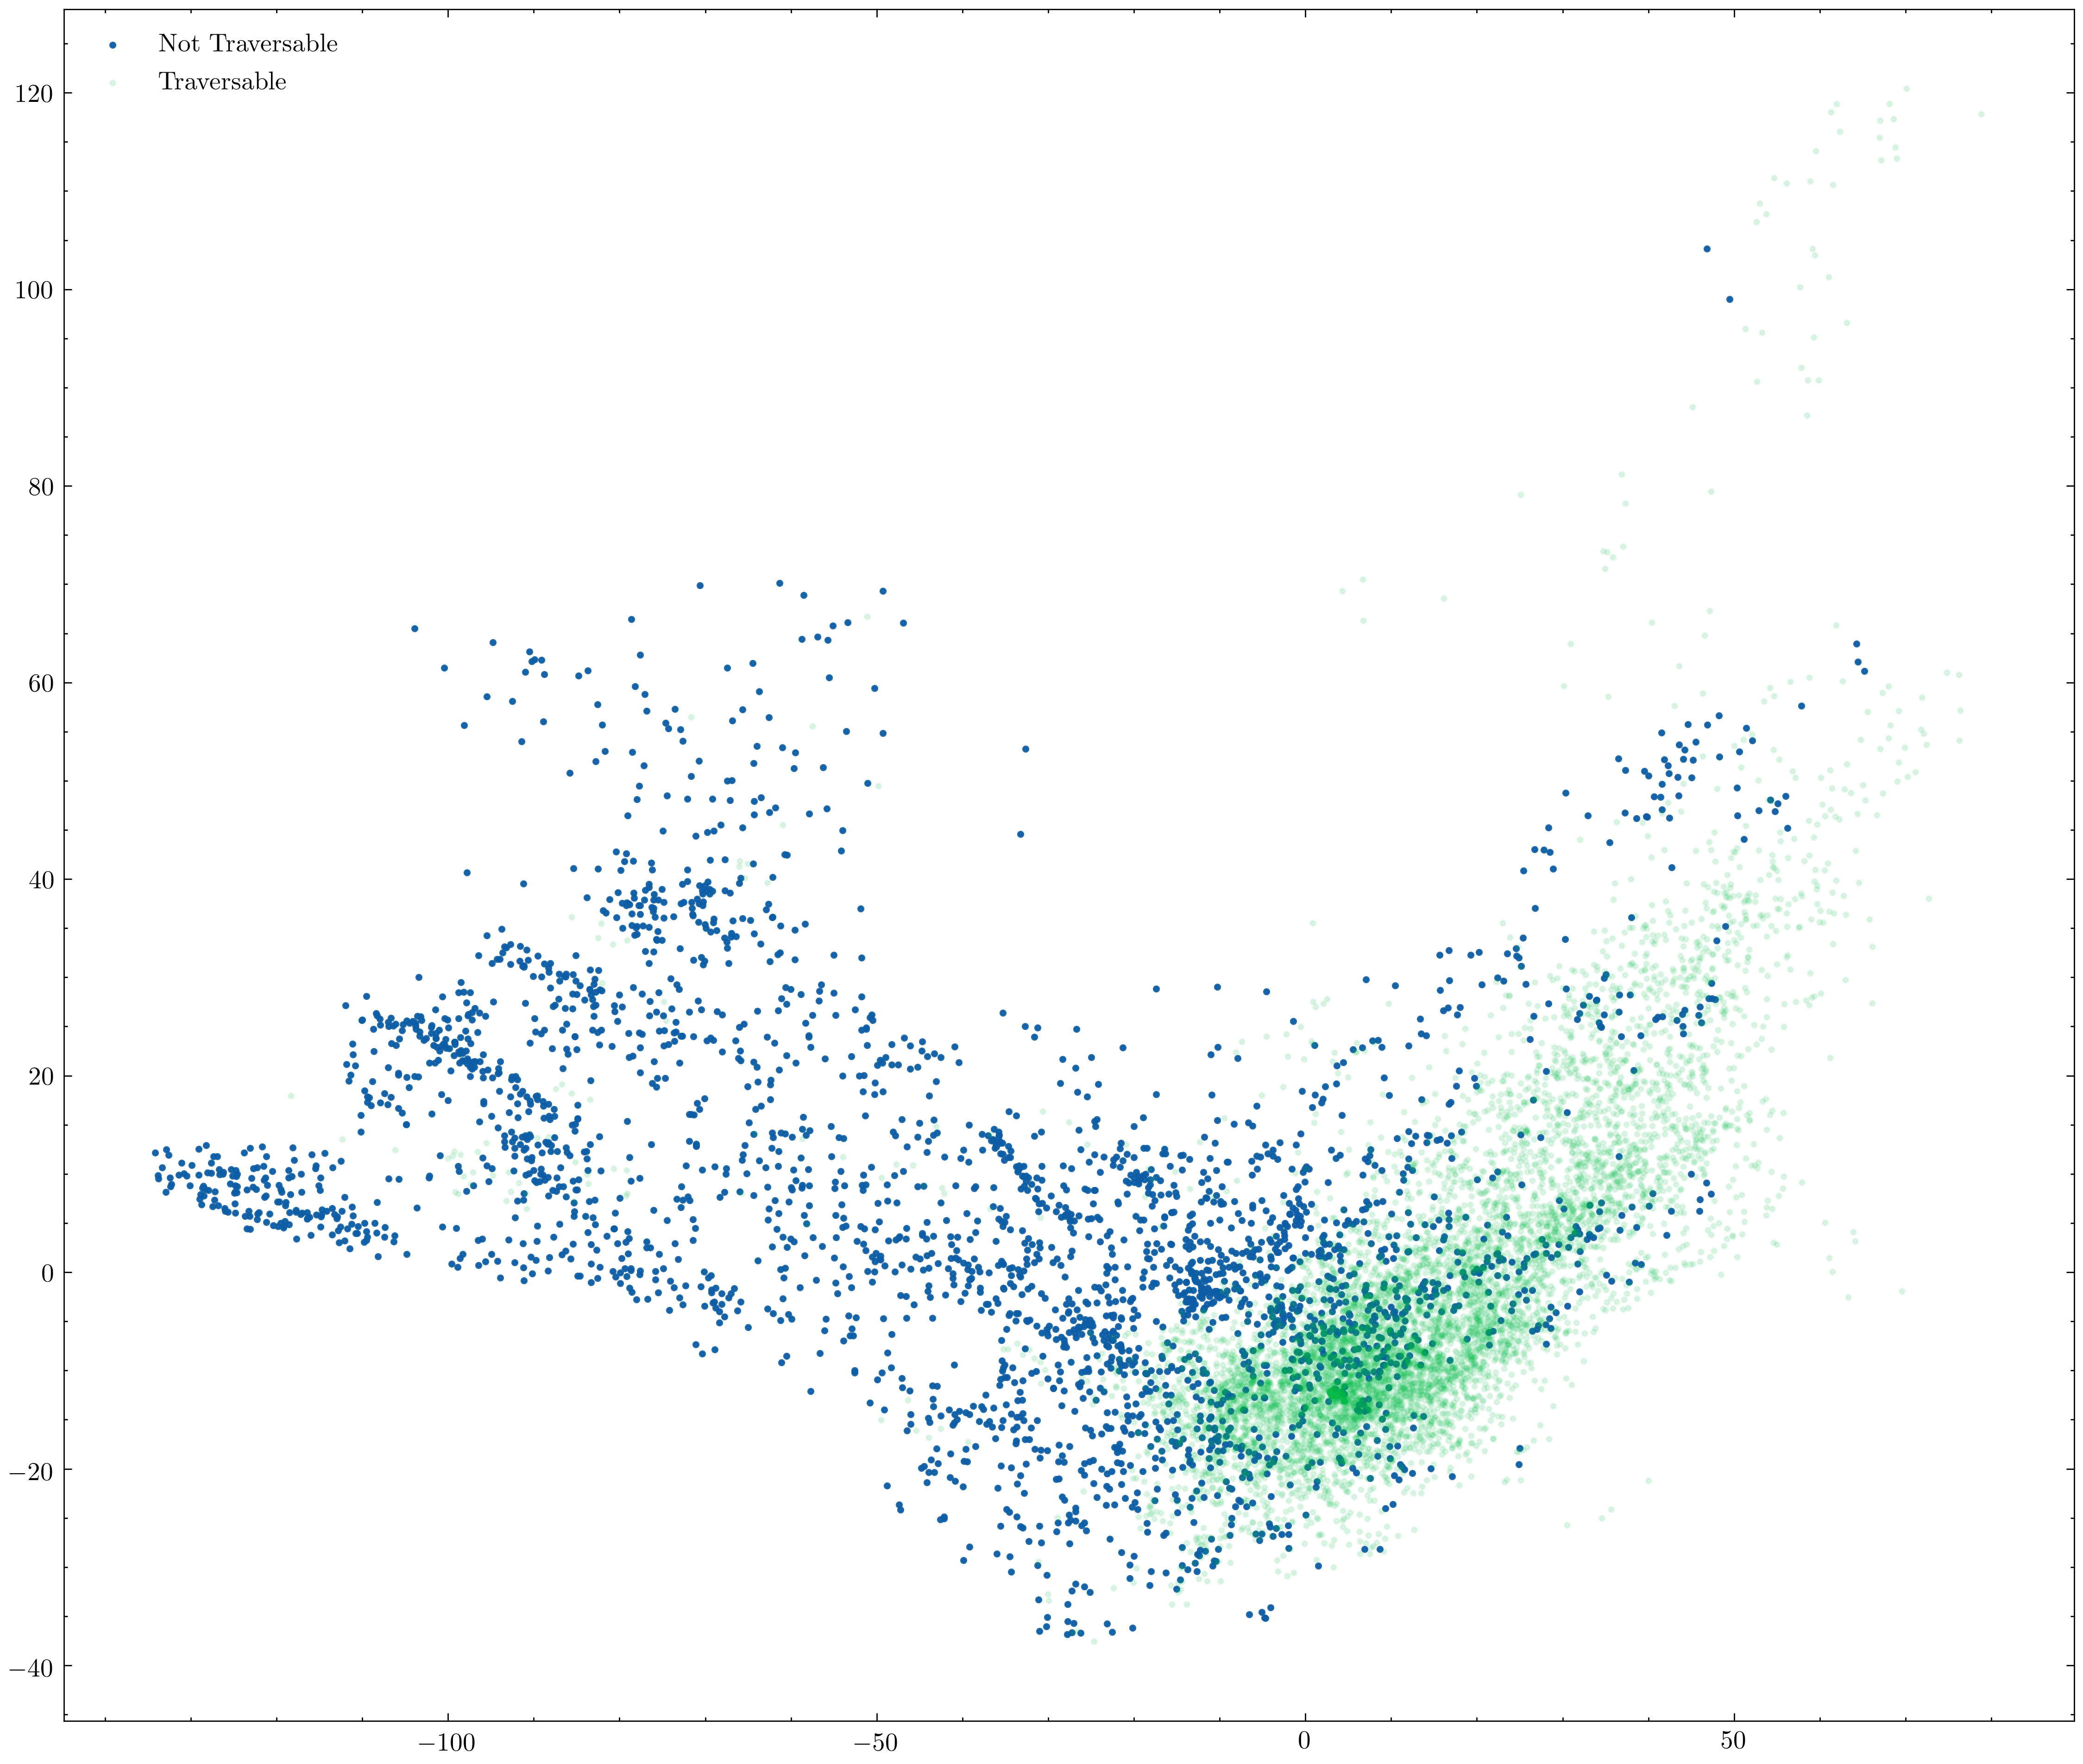
\includegraphics[width=\linewidth]{../img/5/pca/pca-test-0.png}
    \end{subfigure}
    \begin{subfigure}[b]{0.48\textwidth}
        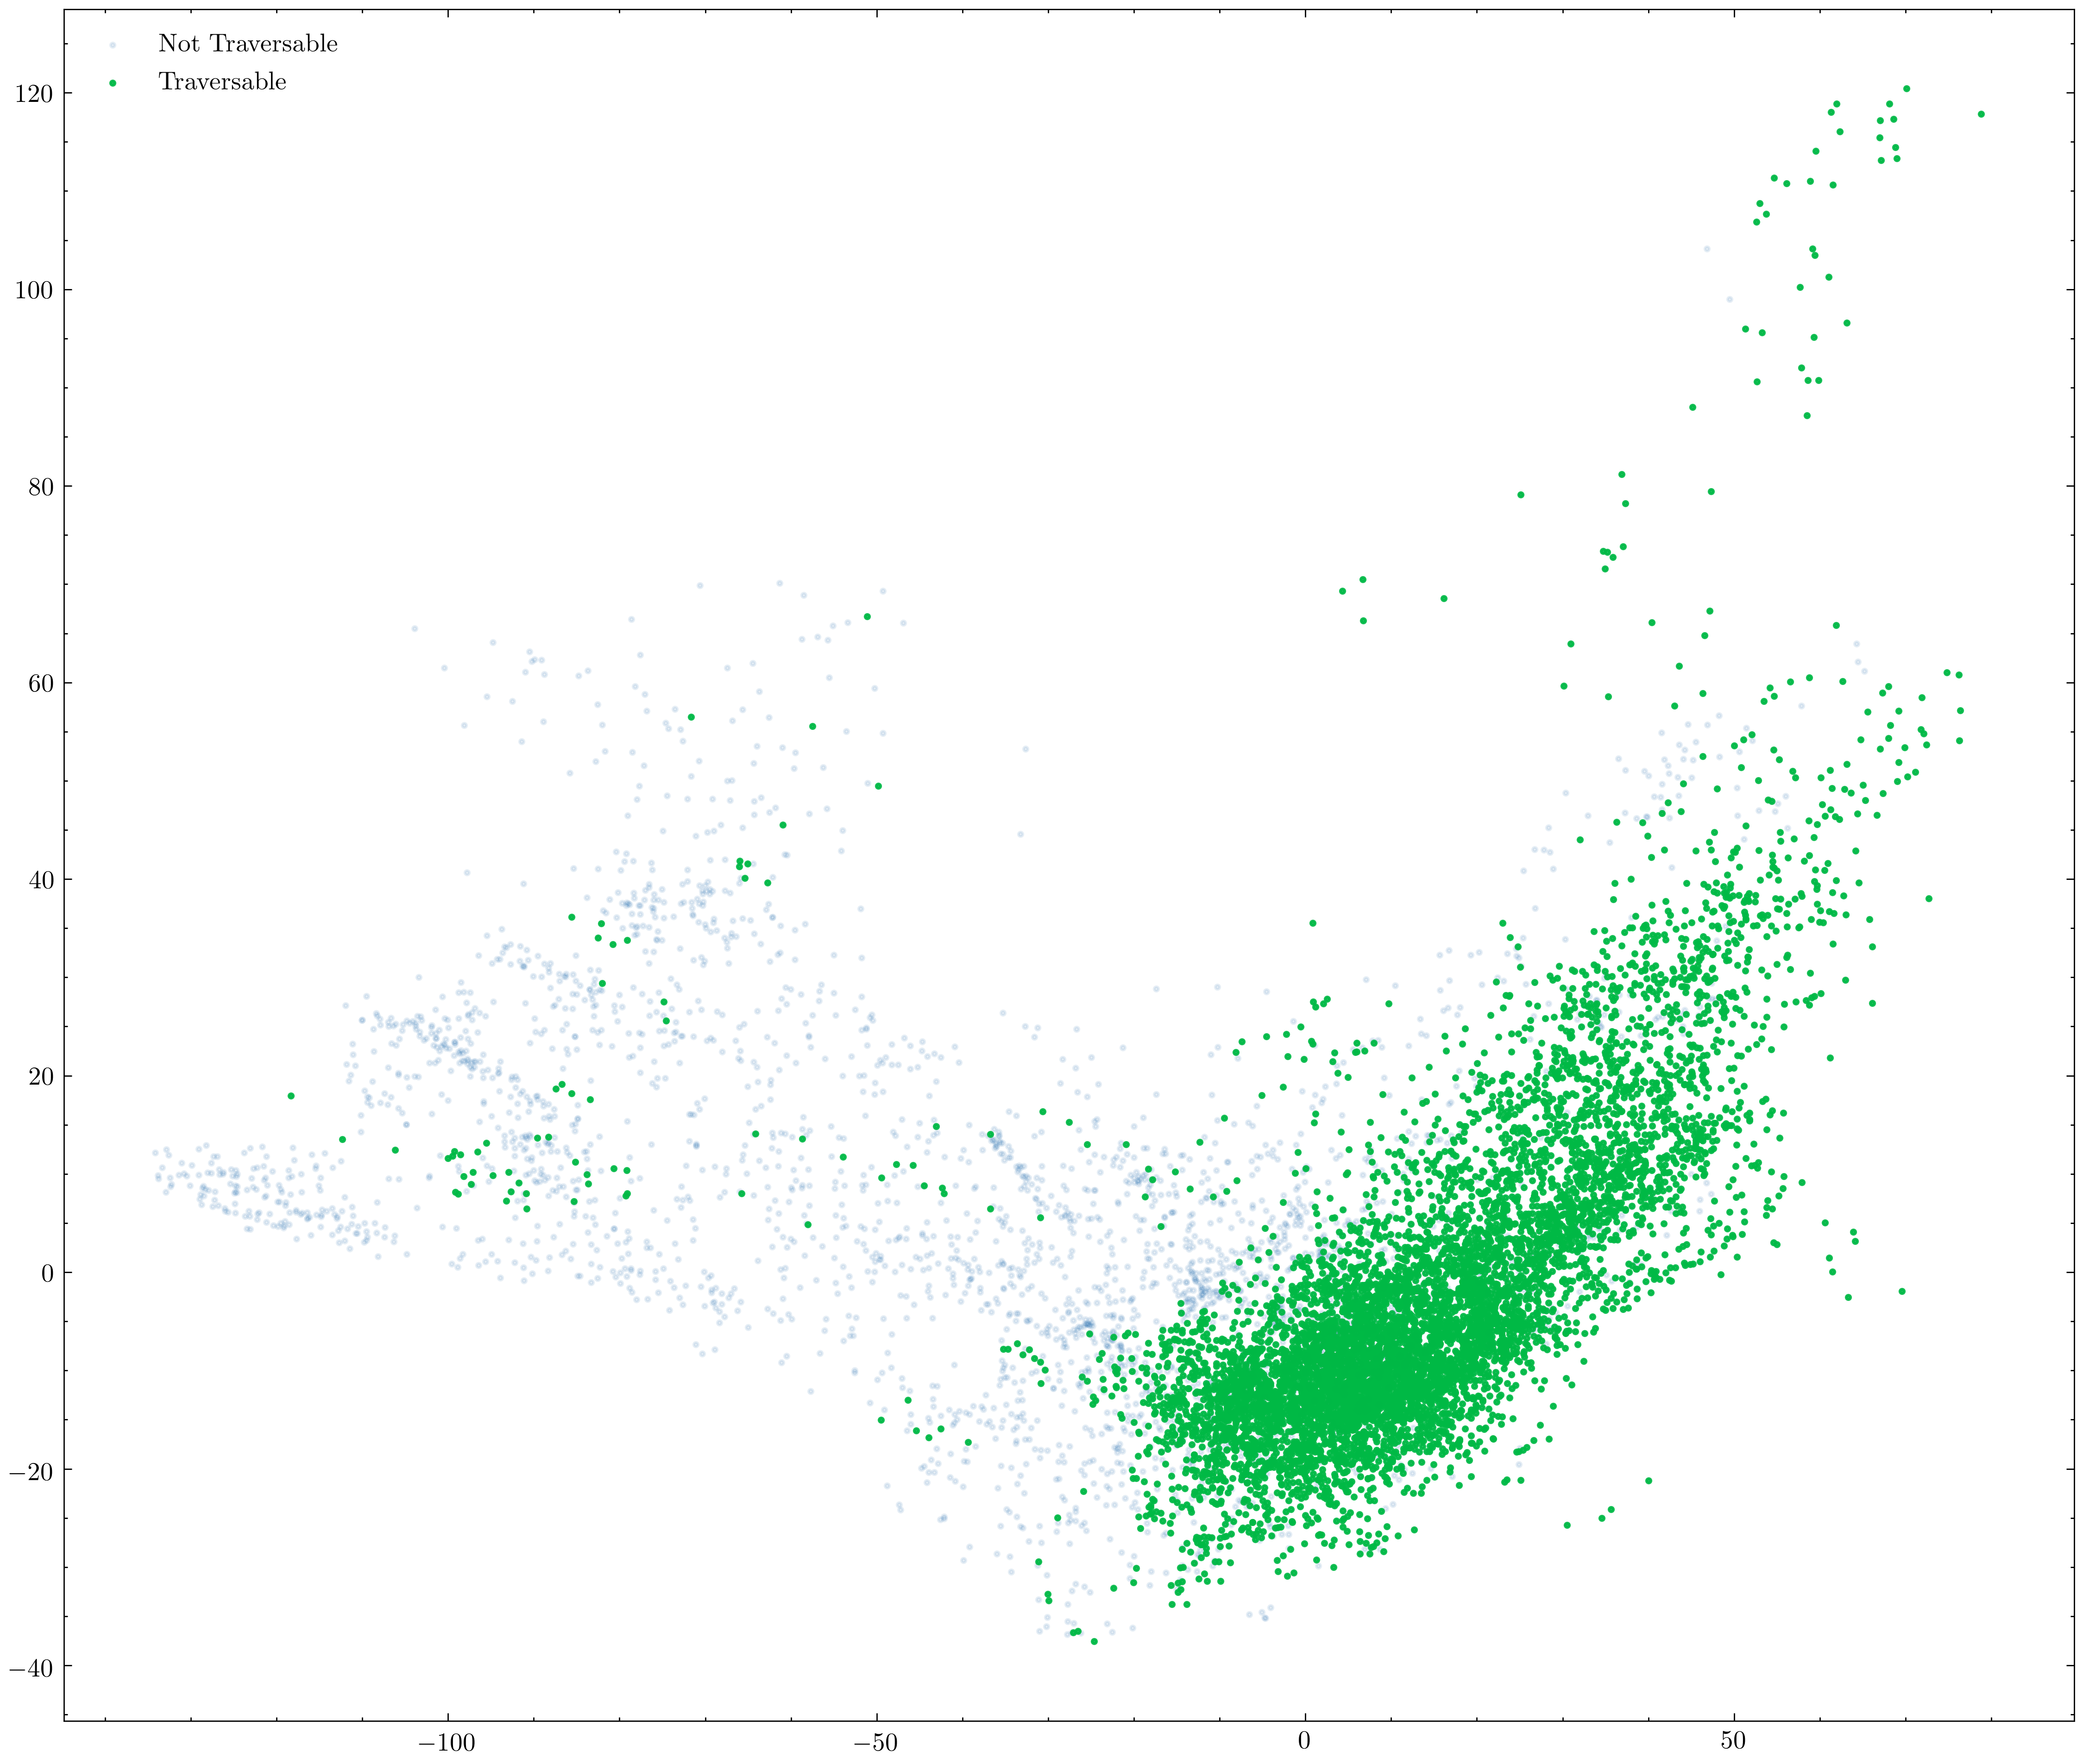
\includegraphics[width=\linewidth]{../img/5/pca/pca-test-1.png}
    \end{subfigure}
\caption{TODO}
\end{figure}
Interesting, the traversable patches are really close to each other, while the others spans a very big surface. This means that there are lots of different terrains with different features that are not traversable. The traversable points are clustered near the center. Moreover, some points are not perfect separable. We plotted the density for each class to better understand where the most points are clusted,
\begin{figure}[H]
\begin{subfigure}[b]{0.48\textwidth}
    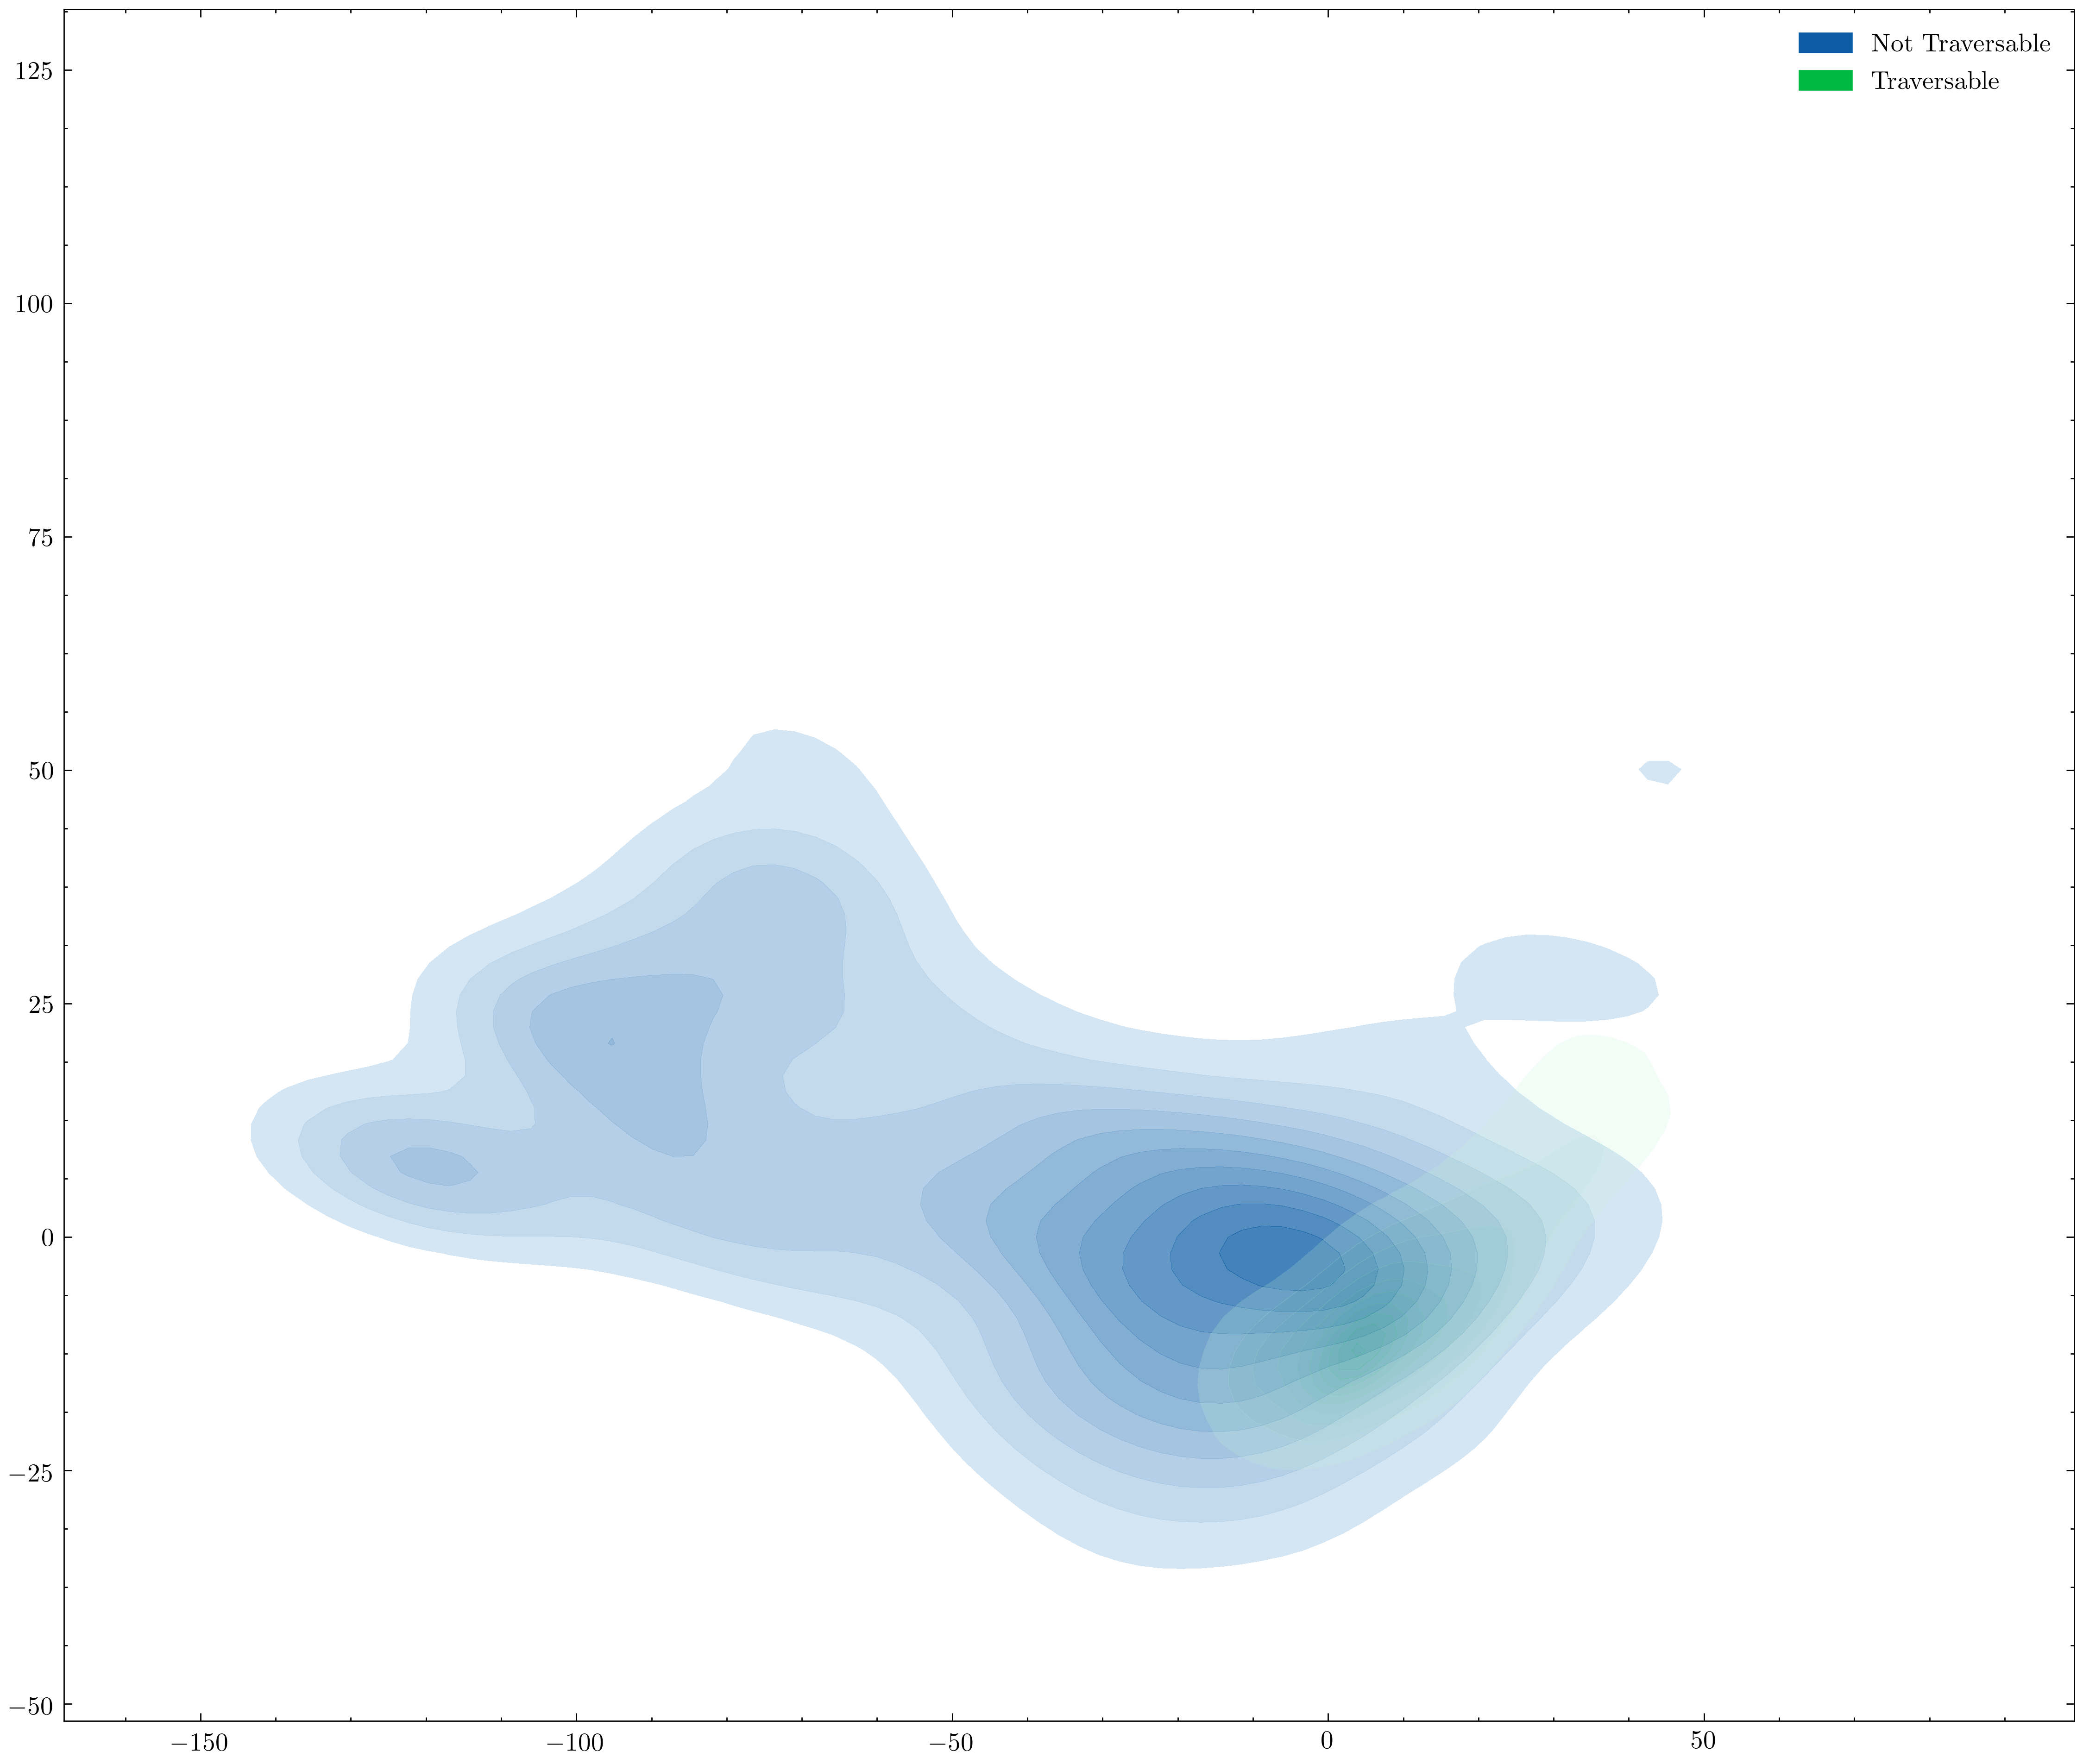
\includegraphics[width=\linewidth]{../img/5/pca/pca-test-0-density.png}
    \caption{Not Traversable}
\end{subfigure}
\begin{subfigure}[b]{0.48\textwidth}
    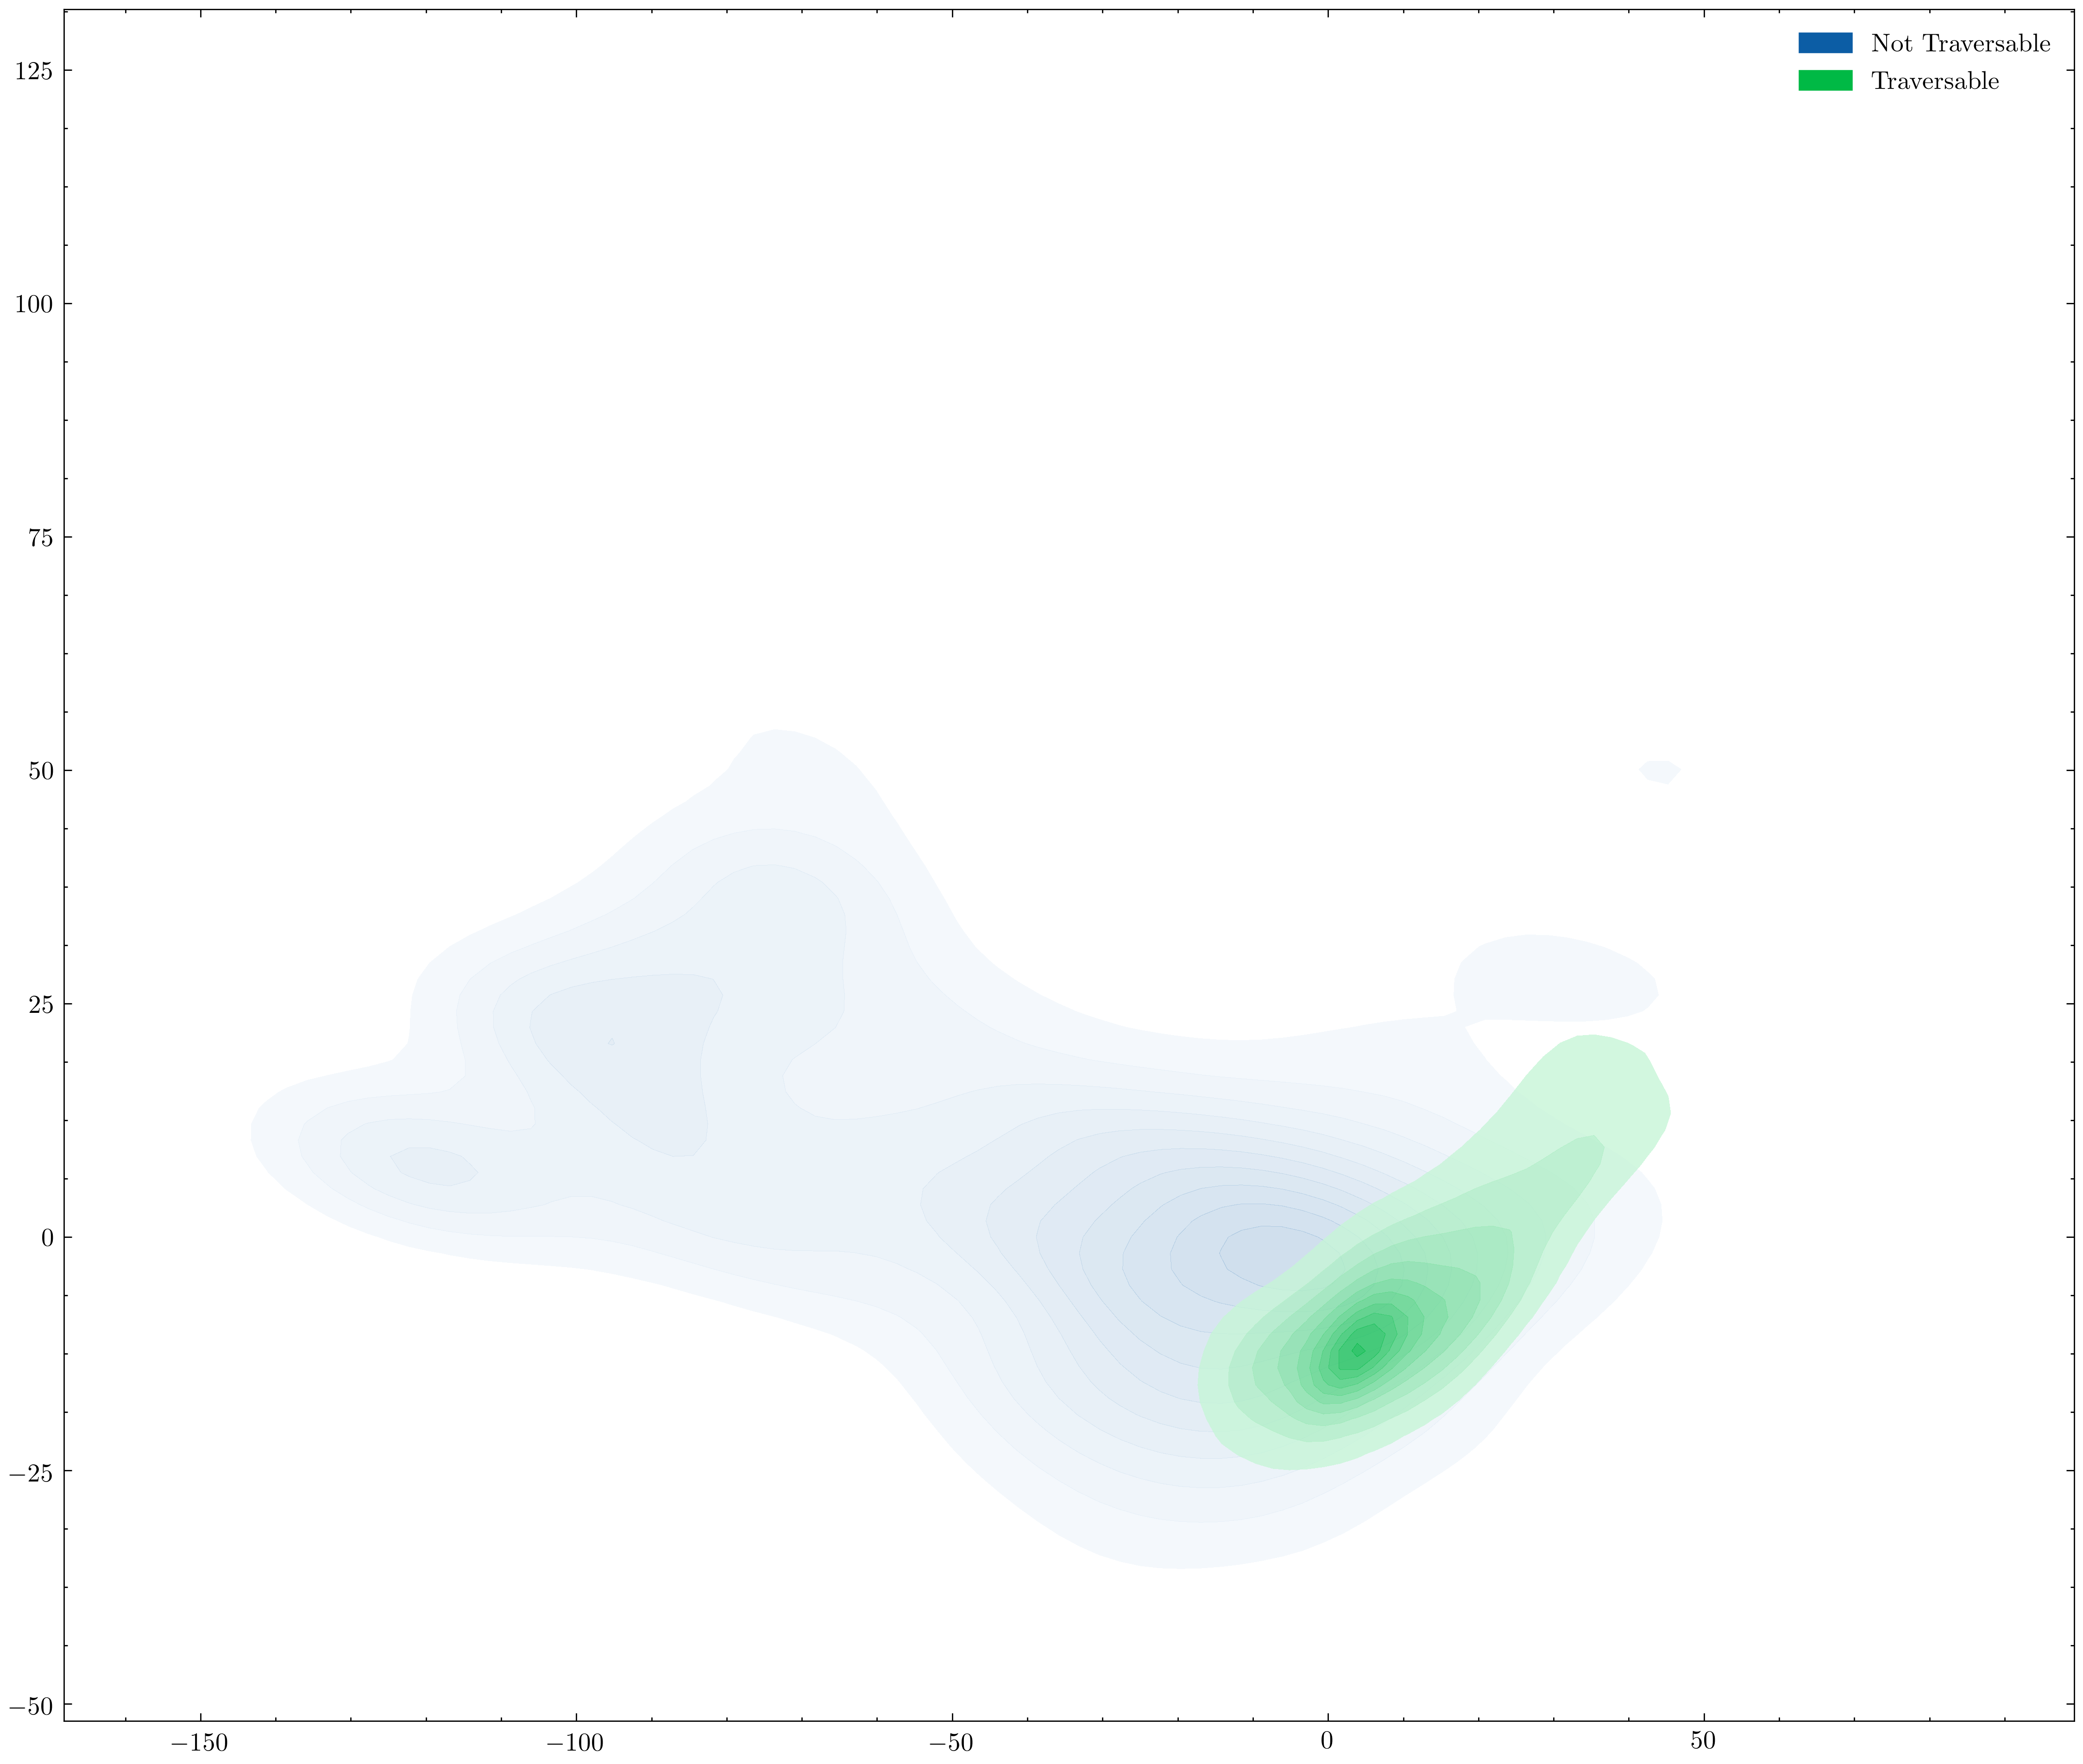
\includegraphics[width=\linewidth]{../img/5/pca/pca-test-1-density.png}
    \caption{Traversable}
    \label{fig : pca-test-density-1}
\end{subfigure}
\caption{Density plot for the points sampled from the test dataset in the features space. The centers of the cluster are not overlapping yielding a good separability and a correct learning.}
\end{figure}
The two centers are really close to each other, this explain the lower AUC score than the validation set. We can also visualize the patches by plotting them using their features coordinates
\begin{figure}[H]
    \centering
    \begin{subfigure}[b]{1\textwidth}
        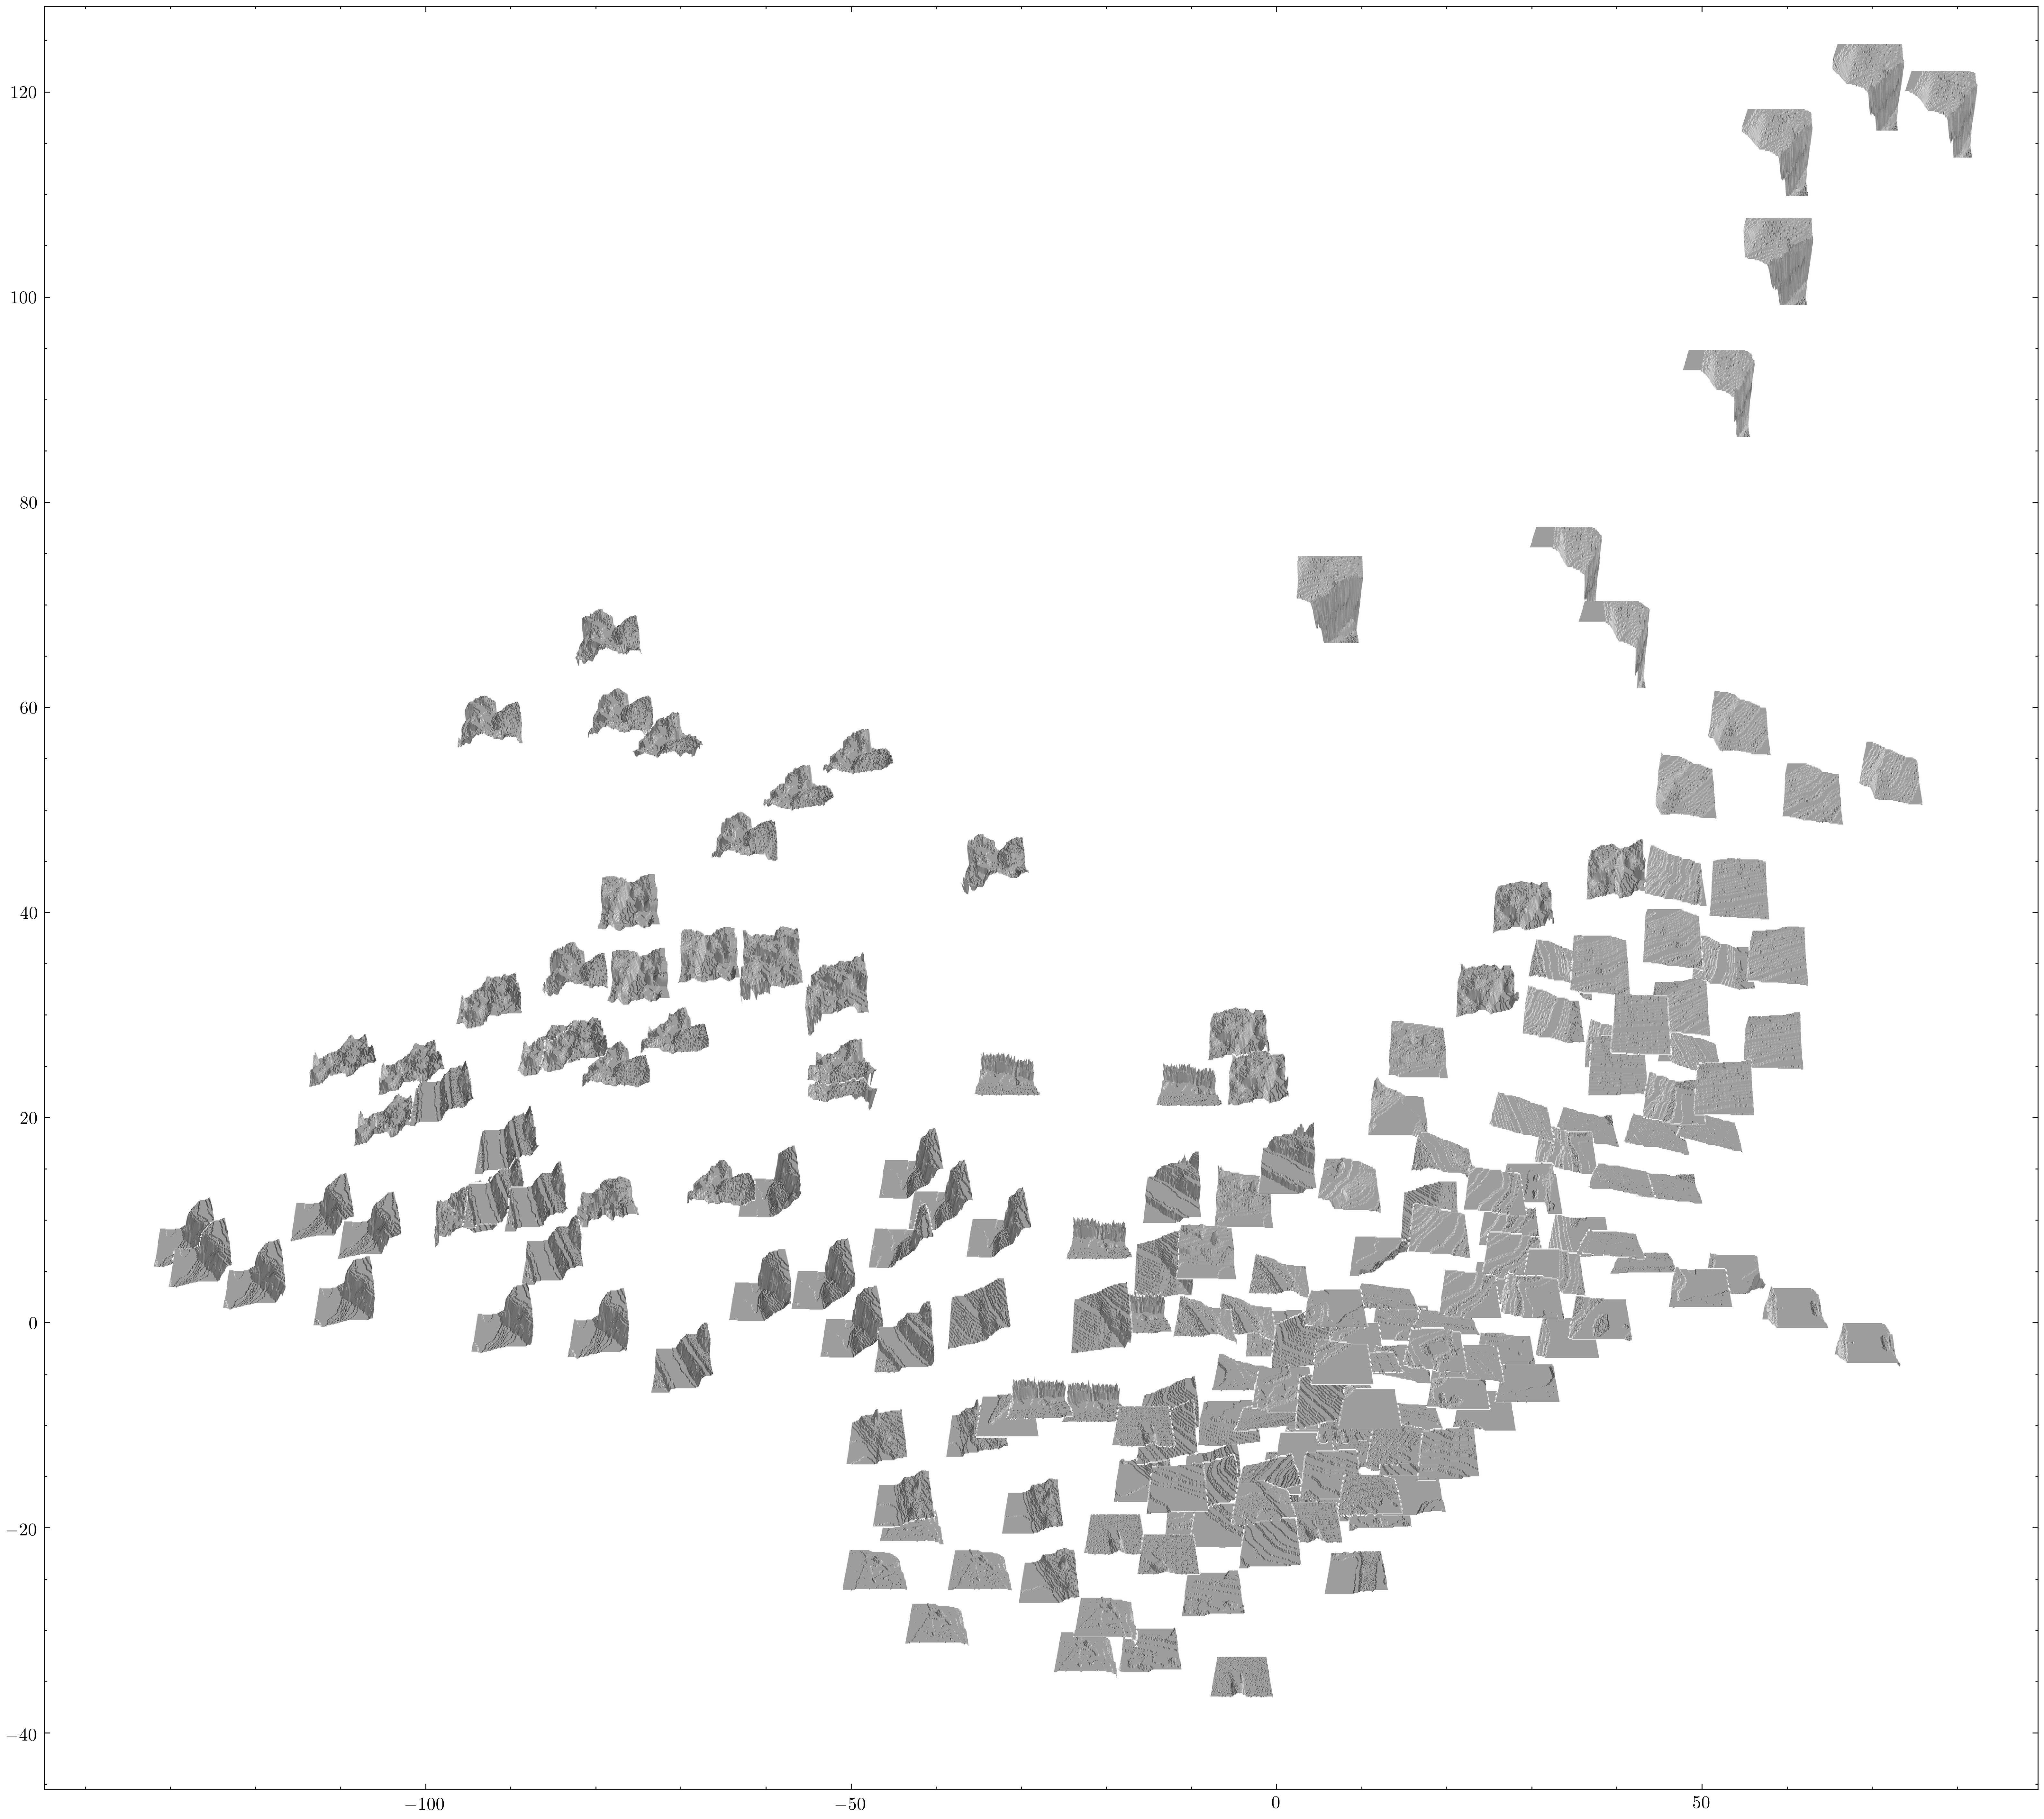
\includegraphics[width=\linewidth]{../img/5/pca/pca-test-patches-200-None-test.png}
    \end{subfigure}
\caption{Patches that cooresponds to coordinates in the features space of the last convolutional layers on the test dataset. Similar grounds are close to each other.}
\ref{fig: pca-test-patches}
\end{figure}
On the top left, from the not traversable cloud, we can see patches with a high level of bumps. Going down we find surfaces with huge walls in front of the robot, while going close to the center we start to see all the traversable patches. Those samples have not too steep slopes. If we move to the density center, green bouble shown in figure \ref{pca-test-density-1}, we encounter lots of flat patches with little obstacles. Going up on the right branch we find downhill and on the top there are falls. 

In the following section we will take a deep look at the test set to find which patches confuse the model. Most probably, those samples will be located between the two clusters center where the difference between classes' features is minimum.
\section{Grad-CAM}
Gradient-weighted Class Activation Mapping (Grad-CAM) \cite{gradcam} is a technique to produce \"visual explanations\" for convolutional neural networks. It highlights the regions of the input image that contribuite the most to the prediciton. 
\begin{figure}[H]
    \centering
    \begin{subfigure}[b]{1\textwidth}
        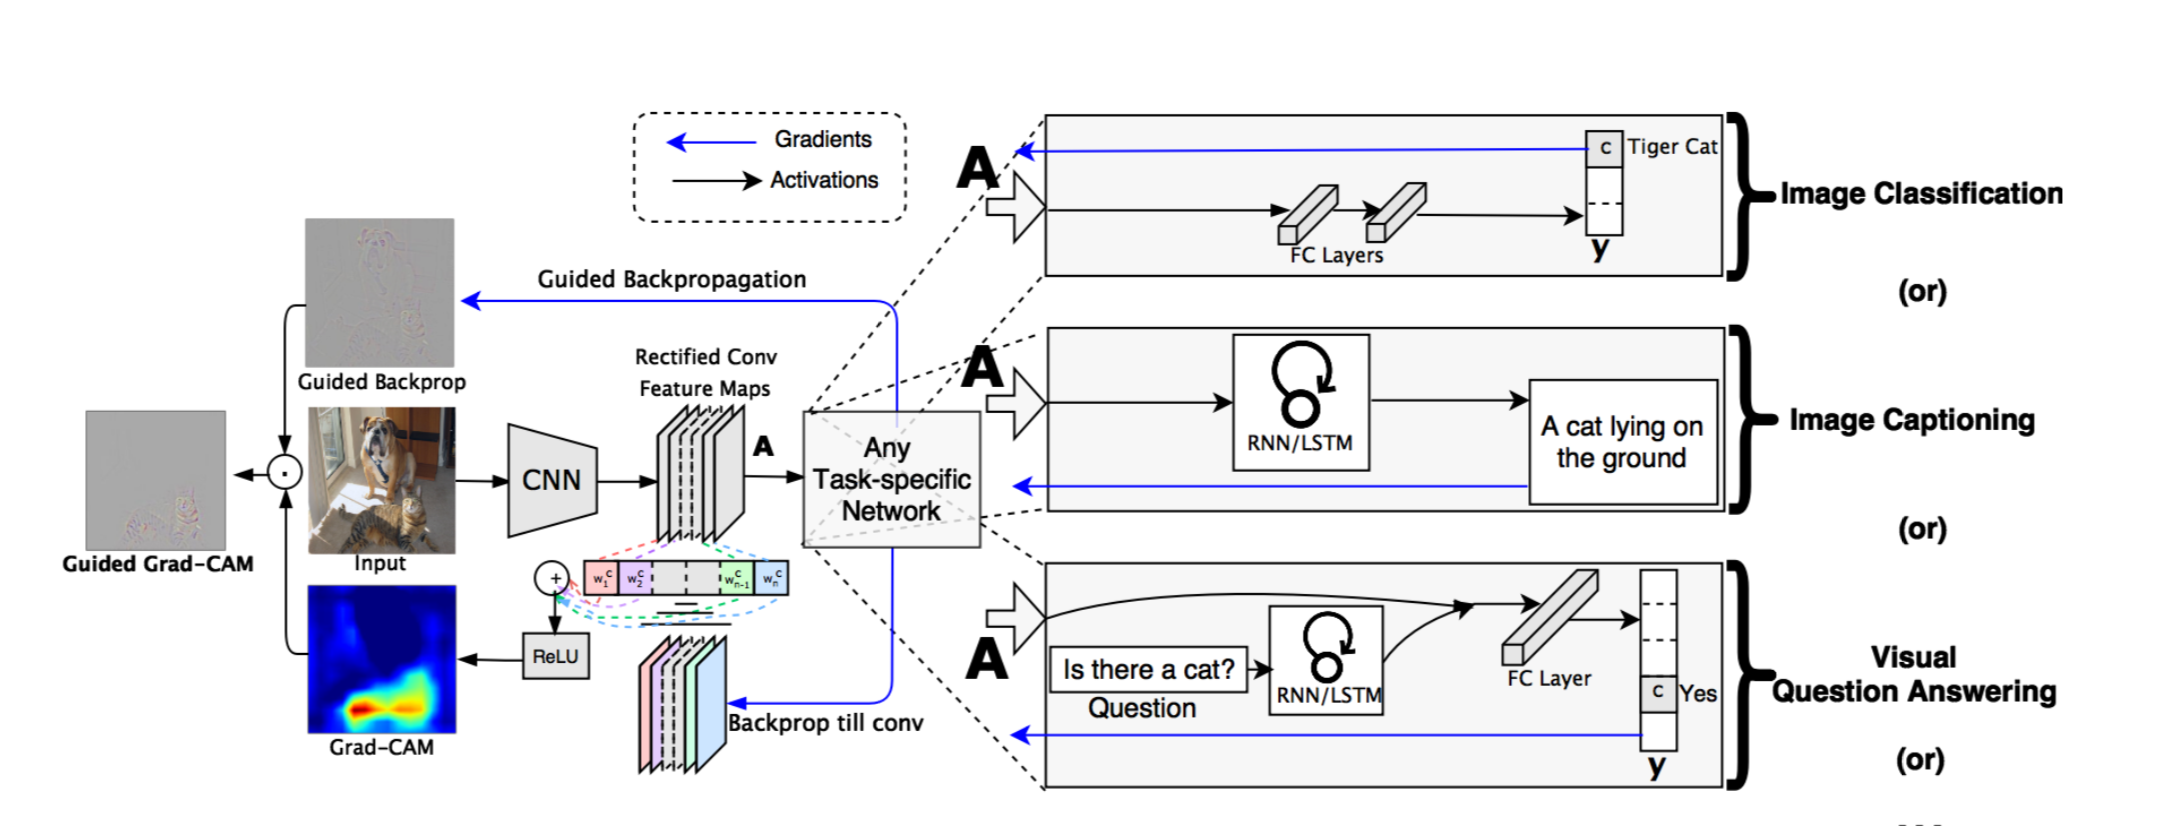
\includegraphics[width=\linewidth]{../img/5/grad_cam1.png}
    \end{subfigure}
\caption{Grad-CAM procedure on an input image. Image from the original paper \cite{gradcam}.}
\end{figure}
In detail, the output with respect to a target class is backpropagate while storing the gradient and the output in the last convolution. Then, global average is applyed to the saved gradient keeping the channel dimension in order to get a 1-d tensor, this will represent the importance of each channel in the target convolutional layer. We  each element of the convolutional layer outputs is multiplyed with the averaged gradients to create the grad cam. This whole procedure is fast and it is architecture independent.

In detail, the output with respect to a target class is backpropagate while storing the gradient and the output in the last convolution. Then global average is applyed the saved gradient keeping the channel dimension in order to get a 1-d tensor, this will represent the importance of each channel in the target convolutional layer. We  each element of the convolutional layer outputs is multiplyed with the averaged gradients to create the grad cam. This whole procedure is fast and it is architecture independent.
% \documentclass[../document.tex]{subfiles}
\begin{document}
\section{Quarry dataset}
\label{sec: quarry-dataset}
After showing the model's capability of correctly separate classes' features we utilized Grad-CAM to visualize some of the samples in the test set. The aim of this section is to show how the model looks at meaningfull features in each inputs to make the prediction even if its prediciton is wrong. For instance, imagine we feed to the model a not traversable patch with an obstacle and the network label is as traversable. Obsliously, the output is wrong but two situation may happened that effect the degree of 'wrongness'. First, the model could just have ignored the obstcle and looked away, meaning if was not even able to understand it should have loook there. Second, the network could have correctly look at the obstacle but thouhgt that maybe the obstacle was not tall enough, showing a correct ability to find and use important features in the map. We showned that, even when the predictions are wrong, our model always look at the most important features of each input to determine its traversability. 

We divided those inputs in four classes based on the model's performance: worst, best, false positive and folse negative. Then, we took twenty inputs from those sets and appplied Grad-CAM as texture on the 3D render to better visualize which region of the inputs caused the prediction. 
% \subsection{Best}
% We start evaluating our model by using the test set composed by samples from the Quarry map. We expect the model to correctly classify the patches with easy to see features such as big obstacles, steep ramps and holes. Unfortunately, the dataset is not trivial and most of the patches are challenging to classify even to human eye. 

% For instance, if look at patches, for some of them is not so easy to estimate the advancement by human eye. This is due to the specific robot locomotion that depends on the starting pose. Our goal in this section is to explain the model predictions on different inputs. 

\subsection{Best}
Best patches have few obstacles. We can obsverse two main clusters of images, flat and slopes. Interesting, when a surface has uneven ground near the left part, so close the the rear legs of the robot, the model is more interesting in those spots, \ref{fig : quarry-best-0}, \ref{fig : quarry-best-2}, \ref{fig : quarry-best-3}, \ref{fig : quarry-best-4}, \ref{fig : quarry-best-15}, \ref{fig : quarry-best-16}, \ref{fig : quarry-best-17}, \ref{fig : quarry-best-18}. This an expected behaviour since if there is an obstacle near the rear legs, then the robot will not be able to advance since it will be stuck from the beginning. 

Moreover, in other patches \ref{fig : quarry-best-1},  \ref{fig : quarry-best-8},  \ref{fig : quarry-best-9},  \ref{fig : quarry-best-19}, the model's also looks ahead of the robot. In those situation the robot is able to properly move at the beginning so the network must evaluate the possibility of obstacles ahead. There are two oblious cases, \ref{fig : quarry-best-8} and  \ref{fig : quarry-best-19}. The first one is a totally flat surface, so the model will look as far as possible to the robot's position to check if there are obstacles. Simarly, in the second, a surface with a bump in the hend, the network controls that spot. So, correctly, the network analysis the first region of the patch that may contain an untraversable obstacle.
\begin{figure}[H]
    \centering
    \begin{subfigure}[b]{0.192\linewidth}
    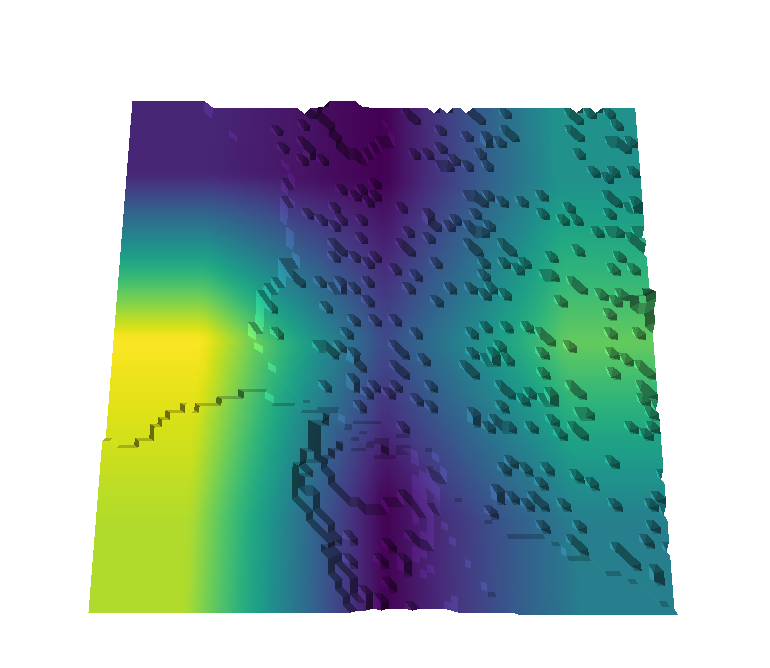
\includegraphics[width=\linewidth]{../img/5/quarry/best/20-patch-3d-majavi-colormap-0.png}
    \caption{0.20cm}
    \label{fig : quarry-best-0}
    \end{subfigure}
    \begin{subfigure}[b]{0.192\linewidth}
    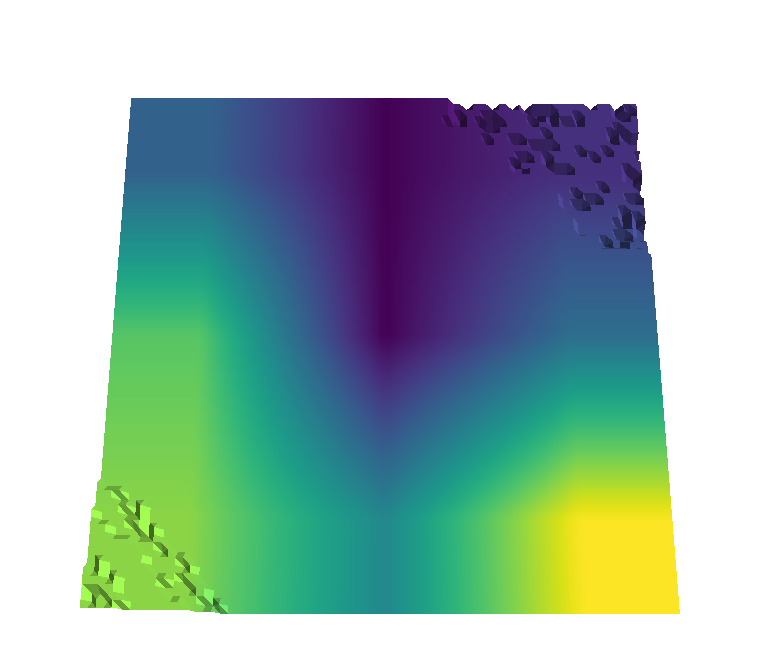
\includegraphics[width=\linewidth]{../img/5/quarry/best/25-patch-3d-majavi-colormap-10.png}
    \caption{0.26cm}
    \label{fig : quarry-best-1}
    \end{subfigure}
    \begin{subfigure}[b]{0.192\linewidth}
    \includegraphics[width=\linewidth]{../img/5/quarry/best/30-patch-3d-majavi-colormap-20.png}
    \caption{0.30cm}
    \label{fig : quarry-best-2}
    \end{subfigure}
    \begin{subfigure}[b]{0.192\linewidth}
    \includegraphics[width=\linewidth]{../img/5/quarry/best/34-patch-3d-majavi-colormap-30.png}
    \caption{0.35cm}
    \label{fig : quarry-best-3}
    \end{subfigure}
    \begin{subfigure}[b]{0.192\linewidth}
    \includegraphics[width=\linewidth]{../img/5/quarry/best/38-patch-3d-majavi-colormap-40.png}
    \caption{0.38cm}
    \label{fig : quarry-best-4}
    \end{subfigure}
    \begin{subfigure}[b]{0.192\linewidth}
    \includegraphics[width=\linewidth]{../img/5/quarry/best/41-patch-3d-majavi-colormap-50.png}
    \caption{0.41cm}
    \label{fig : quarry-best-5}
    \end{subfigure}
    \begin{subfigure}[b]{0.192\linewidth}
    \includegraphics[width=\linewidth]{../img/5/quarry/best/44-patch-3d-majavi-colormap-60.png}
    \caption{0.44cm}
    \label{fig : quarry-best-6}
    \end{subfigure}
    \begin{subfigure}[b]{0.192\linewidth}
    \includegraphics[width=\linewidth]{../img/5/quarry/best/46-patch-3d-majavi-colormap-70.png}
    \caption{0.47cm}
    \label{fig : quarry-best-7}
    \end{subfigure}
    \begin{subfigure}[b]{0.192\linewidth}
    \includegraphics[width=\linewidth]{../img/5/quarry/best/49-patch-3d-majavi-colormap-80.png}
    \caption{0.49cm}
    \label{fig : quarry-best-8}
    \end{subfigure}
    \begin{subfigure}[b]{0.192\linewidth}
    \includegraphics[width=\linewidth]{../img/5/quarry/best/51-patch-3d-majavi-colormap-90.png}
    \caption{0.52cm}
    \label{fig : quarry-best-9}
    \end{subfigure}
    \begin{subfigure}[b]{0.192\linewidth}
    \includegraphics[width=\linewidth]{../img/5/quarry/best/54-patch-3d-majavi-colormap-100.png}
    \caption{0.54cm}
    \label{fig : quarry-best-10}
    \end{subfigure}
    \begin{subfigure}[b]{0.192\linewidth}
    \includegraphics[width=\linewidth]{../img/5/quarry/best/56-patch-3d-majavi-colormap-110.png}
    \caption{0.57cm}
    \label{fig : quarry-best-11}
    \end{subfigure}
    \begin{subfigure}[b]{0.192\linewidth}
    \includegraphics[width=\linewidth]{../img/5/quarry/best/58-patch-3d-majavi-colormap-120.png}
    \caption{0.59cm}
    \label{fig : quarry-best-12}
    \end{subfigure}
    \begin{subfigure}[b]{0.192\linewidth}
    \includegraphics[width=\linewidth]{../img/5/quarry/best/60-patch-3d-majavi-colormap-130.png}
    \caption{0.60cm}
    \label{fig : quarry-best-13}
    \end{subfigure}
    \begin{subfigure}[b]{0.192\linewidth}
    \includegraphics[width=\linewidth]{../img/5/quarry/best/62-patch-3d-majavi-colormap-140.png}
    \caption{0.62cm}
    \label{fig : quarry-best-14}
    \end{subfigure}
    \begin{subfigure}[b]{0.192\linewidth}
    \includegraphics[width=\linewidth]{../img/5/quarry/best/63-patch-3d-majavi-colormap-150.png}
    \caption{0.64cm}
    \label{fig : quarry-best-15}
    \end{subfigure}
    \begin{subfigure}[b]{0.192\linewidth}
    \includegraphics[width=\linewidth]{../img/5/quarry/best/65-patch-3d-majavi-colormap-160.png}
    \caption{0.66cm}
    \label{fig : quarry-best-16}
    \end{subfigure}
    \begin{subfigure}[b]{0.192\linewidth}
    \includegraphics[width=\linewidth]{../img/5/quarry/best/67-patch-3d-majavi-colormap-170.png}
    \caption{0.67cm}
    \label{fig : quarry-best-17}
    \end{subfigure}
    \begin{subfigure}[b]{0.192\linewidth}
    \includegraphics[width=\linewidth]{../img/5/quarry/best/68-patch-3d-majavi-colormap-180.png}
    \caption{0.68cm}
    \label{fig : quarry-best-18}
    \end{subfigure}
    \begin{subfigure}[b]{0.192\linewidth}
    \includegraphics[width=\linewidth]{../img/5/quarry/best/70-patch-3d-majavi-colormap-190.png}
    \caption{0.70cm}
    \label{fig : quarry-best-19}
    \end{subfigure}
    \label{fig : quarry-best}
    \end{figure}

\subsection{Worst}
Those are the not traversable patches, we ordered by advancement. In this case, the region highlighted by the Grad-CAM are the features in the ground that contribute the most to make the patch not traversable. For instance, in some patches, \ref{fig : quarry-worst-1}, \ref{fig : quarry-worst-5}, \ref{fig : quarry-worst-19}, the most not traversable features is directly under the robot legs, similar as before. While, for the others samples, \ref{fig : quarry-worst-0}, \ref{fig : quarry-worst-2}, \ref{fig : quarry-worst-3}, \ref{fig : quarry-worst-4}, ..., the attention of the network is on the obstacles in front of the robot. This is oblious in  \ref{fig : quarry-worst-2}, \ref{fig : quarry-worst-2}, \ref{fig : quarry-worst-4}, where the big wall on the right is almost totally highlighted. So, also in this case, the model is able to understand which part of the patch cause the prediciton. 
\begin{figure}[H]
    \centering
    \begin{subfigure}[b]{0.192\linewidth}
    \includegraphics[width=\linewidth]{../img/5/quarry/worst/-35-patch-3d-majavi-colormap-0.png}
    \caption{-0.36cm}
    \label{fig : quarry-worst-0}
    \end{subfigure}
    \begin{subfigure}[b]{0.192\linewidth}
    \includegraphics[width=\linewidth]{../img/5/quarry/worst/-7-patch-3d-majavi-colormap-10.png}
    \caption{-0.08cm}
    \label{fig : quarry-worst-1}
    \end{subfigure}
    \begin{subfigure}[b]{0.192\linewidth}
    \includegraphics[width=\linewidth]{../img/5/quarry/worst/-4-patch-3d-majavi-colormap-20.png}
    \caption{-0.05cm}
    \label{fig : quarry-worst-2}
    \end{subfigure}
    \begin{subfigure}[b]{0.192\linewidth}
    \includegraphics[width=\linewidth]{../img/5/quarry/worst/-3-patch-3d-majavi-colormap-30.png}
    \caption{-0.03cm}
    \label{fig : quarry-worst-3}
    \end{subfigure}
    \begin{subfigure}[b]{0.192\linewidth}
    \includegraphics[width=\linewidth]{../img/5/quarry/worst/-2-patch-3d-majavi-colormap-40.png}
    \caption{-0.02cm}
    \label{fig : quarry-worst-4}
    \end{subfigure}
    \begin{subfigure}[b]{0.192\linewidth}
    \includegraphics[width=\linewidth]{../img/5/quarry/worst/-1-patch-3d-majavi-colormap-50.png}
    \caption{-0.01cm}
    \label{fig : quarry-worst-5}
    \end{subfigure}
    \begin{subfigure}[b]{0.192\linewidth}
    \includegraphics[width=\linewidth]{../img/5/quarry/worst/00-patch-3d-majavi-colormap-60.png}
    \caption{-0.01cm}
    \label{fig : quarry-worst-6}
    \end{subfigure}
    \begin{subfigure}[b]{0.192\linewidth}
    \includegraphics[width=\linewidth]{../img/5/quarry/worst/00-patch-3d-majavi-colormap-70.png}
    \caption{0.00cm}
    \label{fig : quarry-worst-7}
    \end{subfigure}
    \begin{subfigure}[b]{0.192\linewidth}
    \includegraphics[width=\linewidth]{../img/5/quarry/worst/00-patch-3d-majavi-colormap-80.png}
    \caption{0.01cm}
    \label{fig : quarry-worst-8}
    \end{subfigure}
    \begin{subfigure}[b]{0.192\linewidth}
    \includegraphics[width=\linewidth]{../img/5/quarry/worst/01-patch-3d-majavi-colormap-90.png}
    \caption{0.02cm}
    \label{fig : quarry-worst-9}
    \end{subfigure}
    \begin{subfigure}[b]{0.192\linewidth}
    \includegraphics[width=\linewidth]{../img/5/quarry/worst/02-patch-3d-majavi-colormap-100.png}
    \caption{0.02cm}
    \label{fig : quarry-worst-10}
    \end{subfigure}
    \begin{subfigure}[b]{0.192\linewidth}
    \includegraphics[width=\linewidth]{../img/5/quarry/worst/03-patch-3d-majavi-colormap-110.png}
    \caption{0.03cm}
    \label{fig : quarry-worst-11}
    \end{subfigure}
    \begin{subfigure}[b]{0.192\linewidth}
    \includegraphics[width=\linewidth]{../img/5/quarry/worst/04-patch-3d-majavi-colormap-120.png}
    \caption{0.05cm}
    \label{fig : quarry-worst-12}
    \end{subfigure}
    \begin{subfigure}[b]{0.192\linewidth}
    \includegraphics[width=\linewidth]{../img/5/quarry/worst/06-patch-3d-majavi-colormap-130.png}
    \caption{0.06cm}
    \label{fig : quarry-worst-13}
    \end{subfigure}
    \begin{subfigure}[b]{0.192\linewidth}
    \includegraphics[width=\linewidth]{../img/5/quarry/worst/07-patch-3d-majavi-colormap-140.png}
    \caption{0.08cm}
    \label{fig : quarry-worst-14}
    \end{subfigure}
    \begin{subfigure}[b]{0.192\linewidth}
    \includegraphics[width=\linewidth]{../img/5/quarry/worst/09-patch-3d-majavi-colormap-150.png}
    \caption{0.10cm}
    \label{fig : quarry-worst-15}
    \end{subfigure}
    \begin{subfigure}[b]{0.192\linewidth}
    \includegraphics[width=\linewidth]{../img/5/quarry/worst/11-patch-3d-majavi-colormap-160.png}
    \caption{0.11cm}
    \label{fig : quarry-worst-16}
    \end{subfigure}
    \begin{subfigure}[b]{0.192\linewidth}
    \includegraphics[width=\linewidth]{../img/5/quarry/worst/13-patch-3d-majavi-colormap-170.png}
    \caption{0.13cm}
    \label{fig : quarry-worst-17}
    \end{subfigure}
    \begin{subfigure}[b]{0.192\linewidth}
    \includegraphics[width=\linewidth]{../img/5/quarry/worst/15-patch-3d-majavi-colormap-180.png}
    \caption{0.15cm}
    \label{fig : quarry-worst-18}
    \end{subfigure}
    \begin{subfigure}[b]{0.192\linewidth}
    \includegraphics[width=\linewidth]{../img/5/quarry/worst/17-patch-3d-majavi-colormap-190.png}
    \caption{0.17cm}
    \label{fig : quarry-worst-19}
    \end{subfigure}
    % \begin{subfigure}[b]{0.192\linewidth}
    % \includegraphics[width=\linewidth]{../img/5/quarry/worst/19-patch-3d-majavi-colormap-200.png}
    % \caption{0.20cm}
    % \label{fig : quarry-worst-20}
    % \end{subfigure}
    \label{fig : quarry-worst}
    \end{figure}

\subsection{False Negative}
Those are the inputs that were labeled as negative but predicted as positive. There are lots of interesting cases, we can cluster those patches in three groups: obstacles ahead, slopes and wall parallele to the robot. In figures \ref{fig : quarry-false_negative-0}, \ref{fig : quarry-false_negative-5}, \ref{fig : quarry-false_negative-13}, the models is looking at the obstacle in front of the robot.  Slopes, figures \ref{fig : quarry-false_negative-1}, \ref{fig : quarry-false_negative-8}, \ref{fig : quarry-false_negative-11}, \ref{fig : quarry-false_negative-14}, \ref{fig : quarry-false_negative-15}, \ref{fig : quarry-false_negative-19}, are not completely smooth, making harder to classify them. The last cluster of inputs are the ones with a wall parallel to the robot, figures \ref{fig : quarry-false_negative-13} and \ref{fig : quarry-false_negative-19}. In those cases the model looks at the initial position of the robot, left, and the final part of the patch. Intuitivelly, is trying to understand if the robot fits on the trail. 

In general, most of the region of interested on those patches are located on the left, close to the position of the robot's leg. Correctly, even if the prediction is wrong, the model looks at the first region of the surface, located near the legs, that can cause non traversability. This shown a correct behaviour even with wrongly prediciton meaning that the network is always looking in the correct spot. 
\begin{figure}[H]
\centering
\begin{subfigure}[b]{0.192\linewidth}
\includegraphics[width=\linewidth]{../img/5/quarry/false_negative/-14-patch-3d-majavi-colormap-0.png}
\caption{-0.14cm}
\label{fig : quarry-false_negative-0}
\end{subfigure}
\begin{subfigure}[b]{0.192\linewidth}
\includegraphics[width=\linewidth]{../img/5/quarry/false_negative/-6-patch-3d-majavi-colormap-10.png}
\caption{-0.07cm}
\label{fig : quarry-false_negative-1}
\end{subfigure}
\begin{subfigure}[b]{0.192\linewidth}
\includegraphics[width=\linewidth]{../img/5/quarry/false_negative/-4-patch-3d-majavi-colormap-20.png}
\caption{-0.05cm}
\label{fig : quarry-false_negative-2}
\end{subfigure}
\begin{subfigure}[b]{0.192\linewidth}
\includegraphics[width=\linewidth]{../img/5/quarry/false_negative/-2-patch-3d-majavi-colormap-30.png}
\caption{-0.02cm}
\label{fig : quarry-false_negative-3}
\end{subfigure}
\begin{subfigure}[b]{0.192\linewidth}
\includegraphics[width=\linewidth]{../img/5/quarry/false_negative/00-patch-3d-majavi-colormap-40.png}
\caption{-0.00cm}
\label{fig : quarry-false_negative-4}
\end{subfigure}
\begin{subfigure}[b]{0.192\linewidth}
\includegraphics[width=\linewidth]{../img/5/quarry/false_negative/01-patch-3d-majavi-colormap-50.png}
\caption{0.01cm}
\label{fig : quarry-false_negative-5}
\end{subfigure}
\begin{subfigure}[b]{0.192\linewidth}
\includegraphics[width=\linewidth]{../img/5/quarry/false_negative/02-patch-3d-majavi-colormap-60.png}
\caption{0.03cm}
\label{fig : quarry-false_negative-6}
\end{subfigure}
\begin{subfigure}[b]{0.192\linewidth}
\includegraphics[width=\linewidth]{../img/5/quarry/false_negative/04-patch-3d-majavi-colormap-70.png}
\caption{0.04cm}
\label{fig : quarry-false_negative-7}
\end{subfigure}
\begin{subfigure}[b]{0.192\linewidth}
\includegraphics[width=\linewidth]{../img/5/quarry/false_negative/05-patch-3d-majavi-colormap-80.png}
\caption{0.06cm}
\label{fig : quarry-false_negative-8}
\end{subfigure}
\begin{subfigure}[b]{0.192\linewidth}
\includegraphics[width=\linewidth]{../img/5/quarry/false_negative/06-patch-3d-majavi-colormap-90.png}
\caption{0.07cm}
\label{fig : quarry-false_negative-9}
\end{subfigure}
\begin{subfigure}[b]{0.192\linewidth}
\includegraphics[width=\linewidth]{../img/5/quarry/false_negative/08-patch-3d-majavi-colormap-100.png}
\caption{0.08cm}
\label{fig : quarry-false_negative-10}
\end{subfigure}
\begin{subfigure}[b]{0.192\linewidth}
\includegraphics[width=\linewidth]{../img/5/quarry/false_negative/09-patch-3d-majavi-colormap-110.png}
\caption{0.09cm}
\label{fig : quarry-false_negative-11}
\end{subfigure}
\begin{subfigure}[b]{0.192\linewidth}
\includegraphics[width=\linewidth]{../img/5/quarry/false_negative/10-patch-3d-majavi-colormap-120.png}
\caption{0.11cm}
\label{fig : quarry-false_negative-12}
\end{subfigure}
\begin{subfigure}[b]{0.192\linewidth}
\includegraphics[width=\linewidth]{../img/5/quarry/false_negative/11-patch-3d-majavi-colormap-130.png}
\caption{0.12cm}
\label{fig : quarry-false_negative-13}
\end{subfigure}
\begin{subfigure}[b]{0.192\linewidth}
\includegraphics[width=\linewidth]{../img/5/quarry/false_negative/12-patch-3d-majavi-colormap-140.png}
\caption{0.13cm}
\label{fig : quarry-false_negative-14}
\end{subfigure}
\begin{subfigure}[b]{0.192\linewidth}
\includegraphics[width=\linewidth]{../img/5/quarry/false_negative/14-patch-3d-majavi-colormap-150.png}
\caption{0.14cm}
\label{fig : quarry-false_negative-15}
\end{subfigure}
\begin{subfigure}[b]{0.192\linewidth}
\includegraphics[width=\linewidth]{../img/5/quarry/false_negative/15-patch-3d-majavi-colormap-160.png}
\caption{0.15cm}
\label{fig : quarry-false_negative-16}
\end{subfigure}
\begin{subfigure}[b]{0.192\linewidth}
\includegraphics[width=\linewidth]{../img/5/quarry/false_negative/16-patch-3d-majavi-colormap-170.png}
\caption{0.17cm}
\label{fig : quarry-false_negative-17}
\end{subfigure}
\begin{subfigure}[b]{0.192\linewidth}
\includegraphics[width=\linewidth]{../img/5/quarry/false_negative/17-patch-3d-majavi-colormap-180.png}
\caption{0.18cm}
\label{fig : quarry-false_negative-18}
\end{subfigure}
\begin{subfigure}[b]{0.192\linewidth}
\includegraphics[width=\linewidth]{../img/5/quarry/false_negative/18-patch-3d-majavi-colormap-190.png}
\caption{0.18cm}
\label{fig : quarry-false_negative-19}
\end{subfigure}
% \begin{subfigure}[b]{0.192\linewidth}
% \includegraphics[width=\linewidth]{../img/5/quarry/false_negative/19-patch-3d-majavi-colormap-200.png}
% \caption{0.19cm}
% \label{fig : quarry-false_negative-20}
% \end{subfigure}
\label{fig : quarry-false_negative}
\end{figure}

\subsection{False Positive}
Those are the most interesting ones, they are the samples that were labeled as traversable but predicted as not traversable. They includes different types of patches, obstacles ahead, slopes and flat regions. In each case the model looks at meaningfull features in the patches that can effect traversability. In the slopes, \ref{fig : quarry-false_positive-8} and \ref{false_positive-9}, the first part of the surface is highlighted. Similar as before, the model is looking if the rear legs will be able to move and thought that those small steps will cause the robot not advance enough. The same consideration can be done for figure \ref{fig : quarry-false_positive-5}. On the other hand, some inputs. definitely confused the model. For instance, in figures \ref{fig : quarry-false_positive-7} and \ref{fig : quarry-false_positive-18} the model is more interested in the big obstacle on the right part. This lead to classify those patches as not traversable, even if the obstacle is more distant than the treshold, in this case the network was totally confused. Interesting, figure \ref{fig : quarry-false_positive-13} shows an almost identical situation in which the network correctly looks at the initial part of the ground. We can deduce that even if the in almost any cases the network's prediction is caused by the correct part of the inputs, it can be confused by big obstacle near the end.
\begin{figure}[H]
    \centering
    \begin{subfigure}[b]{0.192\linewidth}
    \includegraphics[width=\linewidth]{../img/5/quarry/false_positive/20-patch-3d-majavi-colormap-0.png}
    \caption{0.20cm}
    \label{fig : quarry-false_positive-0}
    \end{subfigure}
    \begin{subfigure}[b]{0.192\linewidth}
    \includegraphics[width=\linewidth]{../img/5/quarry/false_positive/20-patch-3d-majavi-colormap-12.png}
    \caption{0.21cm}
    \label{fig : quarry-false_positive-1}
    \end{subfigure}
    \begin{subfigure}[b]{0.192\linewidth}
    \includegraphics[width=\linewidth]{../img/5/quarry/false_positive/22-patch-3d-majavi-colormap-24.png}
    \caption{0.22cm}
    \label{fig : quarry-false_positive-2}
    \end{subfigure}
    \begin{subfigure}[b]{0.192\linewidth}
    \includegraphics[width=\linewidth]{../img/5/quarry/false_positive/23-patch-3d-majavi-colormap-36.png}
    \caption{0.23cm}
    \label{fig : quarry-false_positive-3}
    \end{subfigure}
    \begin{subfigure}[b]{0.192\linewidth}
    \includegraphics[width=\linewidth]{../img/5/quarry/false_positive/24-patch-3d-majavi-colormap-48.png}
    \caption{0.24cm}
    \label{fig : quarry-false_positive-4}
    \end{subfigure}
    \begin{subfigure}[b]{0.192\linewidth}
    \includegraphics[width=\linewidth]{../img/5/quarry/false_positive/25-patch-3d-majavi-colormap-60.png}
    \caption{0.25cm}
    \label{fig : quarry-false_positive-5}
    \end{subfigure}
    \begin{subfigure}[b]{0.192\linewidth}
    \includegraphics[width=\linewidth]{../img/5/quarry/false_positive/25-patch-3d-majavi-colormap-72.png}
    \caption{0.26cm}
    \label{fig : quarry-false_positive-6}
    \end{subfigure}
    \begin{subfigure}[b]{0.192\linewidth}
    \includegraphics[width=\linewidth]{../img/5/quarry/false_positive/26-patch-3d-majavi-colormap-84.png}
    \caption{0.27cm}
    \label{fig : quarry-false_positive-7}
    \end{subfigure}
    \begin{subfigure}[b]{0.192\linewidth}
    \includegraphics[width=\linewidth]{../img/5/quarry/false_positive/27-patch-3d-majavi-colormap-96.png}
    \caption{0.27cm}
    \label{fig : quarry-false_positive-8}
    \end{subfigure}
    \begin{subfigure}[b]{0.192\linewidth}
    \includegraphics[width=\linewidth]{../img/5/quarry/false_positive/27-patch-3d-majavi-colormap-108.png}
    \caption{0.28cm}
    \label{fig : quarry-false_positive-9}
    \end{subfigure}
    \begin{subfigure}[b]{0.192\linewidth}
    \includegraphics[width=\linewidth]{../img/5/quarry/false_positive/29-patch-3d-majavi-colormap-120.png}
    \caption{0.29cm}
    \label{fig : quarry-false_positive-10}
    \end{subfigure}
    \begin{subfigure}[b]{0.192\linewidth}
    \includegraphics[width=\linewidth]{../img/5/quarry/false_positive/30-patch-3d-majavi-colormap-132.png}
    \caption{0.30cm}
    \label{fig : quarry-false_positive-11}
    \end{subfigure}
    \begin{subfigure}[b]{0.192\linewidth}
    \includegraphics[width=\linewidth]{../img/5/quarry/false_positive/31-patch-3d-majavi-colormap-144.png}
    \caption{0.32cm}
    \label{fig : quarry-false_positive-12}
    \end{subfigure}
    \begin{subfigure}[b]{0.192\linewidth}
    \includegraphics[width=\linewidth]{../img/5/quarry/false_positive/33-patch-3d-majavi-colormap-156.png}
    \caption{0.34cm}
    \label{fig : quarry-false_positive-13}
    \end{subfigure}
    \begin{subfigure}[b]{0.192\linewidth}
    \includegraphics[width=\linewidth]{../img/5/quarry/false_positive/35-patch-3d-majavi-colormap-168.png}
    \caption{0.35cm}
    \label{fig : quarry-false_positive-14}
    \end{subfigure}
    \begin{subfigure}[b]{0.192\linewidth}
    \includegraphics[width=\linewidth]{../img/5/quarry/false_positive/36-patch-3d-majavi-colormap-180.png}
    \caption{0.36cm}
    \label{fig : quarry-false_positive-15}
    \end{subfigure}
    \begin{subfigure}[b]{0.192\linewidth}
    \includegraphics[width=\linewidth]{../img/5/quarry/false_positive/38-patch-3d-majavi-colormap-192.png}
    \caption{0.39cm}
    \label{fig : quarry-false_positive-16}
    \end{subfigure}
    \begin{subfigure}[b]{0.192\linewidth}
    \includegraphics[width=\linewidth]{../img/5/quarry/false_positive/41-patch-3d-majavi-colormap-204.png}
    \caption{0.41cm}
    \label{fig : quarry-false_positive-17}
    \end{subfigure}
    \begin{subfigure}[b]{0.192\linewidth}
    \includegraphics[width=\linewidth]{../img/5/quarry/false_positive/46-patch-3d-majavi-colormap-216.png}
    \caption{0.46cm}
    \label{fig : quarry-false_positive-18}
    \end{subfigure}
    \begin{subfigure}[b]{0.192\linewidth}
    \includegraphics[width=\linewidth]{../img/5/quarry/false_positive/51-patch-3d-majavi-colormap-228.png}
    \caption{0.52cm}
    \label{fig : quarry-false_positive-19}
    \end{subfigure}
    % \begin{subfigure}[b]{0.192\linewidth}
    % \includegraphics[width=\linewidth]{../img/5/quarry/false_positive/61-patch-3d-majavi-colormap-240.png}
    % \caption{0.62cm}
    % \label{fig : quarry-false_positive-20}
    % \end{subfigure}
    \label{fig : quarry-false_positive}
    \end{figure}


\end{document}
\documentclass[./chapter5.tex]{subfiles}
\begin{document}
\section{Robustness}


\end{document}
%

\end{document}

\subfile{./tex/abstract.tex}
\subfile{./tex/introduction.tex}
\subfile{./tex/chapter1.tex}
\subfile{./tex/chapter3.tex}
\subfile{./tex/chapter4.tex}
\subfile{./tex/chapter5.tex}


\printbibliography

\end{document}